\documentclass[11pt,a4paper,leqno,oneside]{book}

\usepackage{surprises}

%\includeonly{}

\begin{document}

\tikzsetfigurename{front}
% !TeX root = surprises.tex

\maketitle

\foreword

\begin{flushright}
\parbox{7cm}{
\begin{footnotesize}
\begin{flushright}
If everyone were exposed to mathematics in its natural state, with all the challenging fun and surprises that that entails, I think we would see a dramatic change both in the attitude of students toward mathematics, and in our conception of what it means to be ``good at math.''\\
Paul Lockhart\mbox{}\\\mbox{}\\
I'm really hungry for surprises because each one makes us ever-so-slightly but substantially smarter.\\
Tadashi Tokieda
\end{flushright}
\end{footnotesize}
}
\end{flushright}

\medskip

Mathematics, when appropriately approached, can provide us with plentiful pleasant surprises. This is confirmed by a Google search of ``mathematical surprises,'' which, surprisingly, yields almost half a billion items. What is a surprise? The origins of the word trace back to Old French with roots in Latin: ``sur'' (over) and ``prendre'' (to take, to grasp, to seize). Literally, to surprise is to overtake. As a noun, surprise is both an unanticipated or bewildering event or circumstance, as well as the emotion caused by it.

Consider, for example, an extract from a lecture by Maxim Bruckheimer\footnote{Maxim Bruckheimer was a mathematician who was one of the founders of the Open University UK and Dean of its Faculty of Mathematics. He was Head of the Department of Science Teaching at the Weizmann Institute of Science.} on the Feuerbach circle: ``Two points lie on one and only one straight line, this is no surprise. However, three points are not necessarily on one straight line and if, during a geometrical exploration, three points `fall into' a straight line, this is a surprise and frequently we need to refer to this fact as a theorem to be proven. Any three points not on a straight line lie on one circle. However, if four points lie on the same circle, this is a surprise that should be formulated as a theorem. \ldots{} Insofar as the number of points on a straight line is larger than $3$, so is the theorem the more surprising. Likewise, insofar as the number of points lying on one circle is larger than $4$, so is the theorem the more surprising. Thus, the statement that for any triangle there are nine related points on the same circle … is very surprising. Moreover, in spite of the magnitude of the surprise, its proof is elegant and easy.''

In this book Mordechai Ben-Ari offers a rich collection of mathematical surprises, most of them less well known than the Feuerbach Circle and with sound reasons for including them. First, in spite of being absent from textbooks, the mathematical gems of this book are accessible with just a high school background (and patience, and paper and pencil, since fun does not come for free). Second, when a mathematical result challenges what we take for granted, we are indeed surprised (Chaps.~\ref{c.collapse}, \ref{c.compass}). Similarly, we are surprised by: the cleverness of an argument (Chaps.~\ref{c.trisect}, \ref{c.square}), the justification of the possibility of a geometric construction by algebraic means (Chap.~\ref{c.heptadecagon}), a proof relying on an apparently unrelated topic (Chaps.~\ref{c.five}, \ref{c.museum}), a strange proof by induction (Chap.~\ref{c.induction}), new ways of looking at a well-known result (Chap.~\ref{c.quadratic}), a seemingly minor theorem becoming the foundation of a whole field of mathematics (Chap.~\ref{c.ramsey}), unexpected sources of inspiration (Chap.~\ref{c.langford}), rich formalizations emerging from purely recreational activities such as origami (Chaps.~\ref{c.origami-axioms}--\ref{c.origami-constructions}). These are all different reasons for the inclusion of the pleasant, beautiful and memorable mathematical surprises in this lovely book.
   
So far I have addressed how the book relates to the first part of the definition of surprise, the cognitive rational reasons for the unexpected. As to the second aspect, the emotional aspect, this book is a vivid instantiation of what many mathematicians claim regarding the primary reason for doing mathematics: it is fascinating! Moreover, they claim that mathematics stimulates both our intellectual curiosity and our esthetic sensibilities, and that solving a problem or understanding a concept provides a spiritual reward, which entices us to keep working on more problems and concepts. 

It has been said that the function of a foreword tell readers why they should read the book. I have tried to accomplish this, but I believe that the fuller answer will come from you, the reader, after reading it and experiencing what the etymology of the word surprise suggests: to be overtaken by it!



\vspace{\baselineskip}
\begin{flushright}
\textit{Abraham Arcavi}
\end{flushright}


\preface

Godfried Toussaint's article on the ``collapsing compass''  \cite{toussaint} made a profound impression on me. It would never have occurred to me that the modern compass with a friction joint is not the one used in Euclid's day. In this book I present a selection of mathematical results that are not only interesting, but that surprised me when I first encountered them.

The mathematics required to read the book is secondary-school mathematics, but that does not mean that the material is simple. Some of the proofs are quite long and require that the reader be willing to persevere in studying the material. The reward is understanding of some of the most beautiful results in mathematics. The book is not a textbook, because the wide range of topics covered doesn't fit neatly into a syllabus. It is appropriate for enrichment activities for secondary-school students, for college-level seminars and for mathematics teachers.

 The chapters can be read independently. (An exception is that Chap.~\ref{c.origami-axioms} on the axioms of origami is a prerequisite for Chaps.~\ref{c.origami-cube},~\ref{c.origami-constructions}, the other chapters on origami.) Notes relevant to all chapters are given below in list labeled Style.

\subsection*{What Is a Surprise?}

There were three criteria for including a topic in the book:
\begin{itemize}
\item The theorem surprised me. Particularly surprising were the theorems on constructibility with a straightedge and compass. The extremely rich mathematics of origami was almost shocking: when a mathematics teacher proposed a project on origami, I initially turned her down because I doubted that there could be any serious mathematics associated with the art form.
Other topics were included because although I knew the results, their proofs were surprising in their elegance and accessibility, in particular, Gauss's purely algebraic proof that a regular heptadecagon can be constructed.

\item The material does not appear in secondary-school and college textbooks, and I have had to read advanced textbooks and the research literature. There are Wikipedia articles on most of the topics, but you have to know where to look and the articles are often outlines.

\item The theorems and proofs are accessible with a good knowledge of secondary-school mathematics.
\end{itemize}
Each chapter concludes with a paragraph \textit{What Is the Surprise?} which explains my choice of the topic.

\subsection*{An Overview of the Contents}

Chapter~\ref{c.collapse} presents Euclid's proof that any construction that is possible with a fixed compass is possible with a collapsing compass. Many proofs have been given, but, as Toussaint shows, most are incorrect because they depend on diagrams which do not always correctly depict the geometry. To emphasize that one must not trust diagrams, I present the famous alleged proof that every triangle is isoceles. 

Over the centuries mathematicians unsuccessfully sought to trisect an arbitrary angle (divide it into three equal parts) using only a straightedge and compass. Underwood Dudley made a comprehensive study of trisectors who find incorrect constructions; most constructions are approximations that are claimed to be accurate. Chapter~\ref{c.trisect} starts by presenting two of these constructions and developing the trigonometric formulas showing that they are only approximations. To show that trisection using just a straightedge and compass is of no practical importance, trisections using more complex tools are presented, Archimedes's \emph{neusis} and Hippias's \emph{quadratrix}. The chapter ends with a proof that it is impossible to trisect an arbitrary angle with a straightedge and compass. 

Squaring a circle (given a circle construct a square with the same area) cannot be performed using a straightedge and compass because the value of $\pi$ cannot be constructed. Chapter~\ref{c.square} presents three elegant constructions of close approximations to $\pi$, one by Kocha\'{n}ski and two by Ramanujan. The chapter concludes by showing that a quadratrix can be used to square a circle.

The four-color theorem states that it is possible to color any planar map with four colors, such that no countries with a common boundary are colored with the same color. The proof of this theorem is extremely complicated, but the proof of the five-color theorem is elementary and elegant, as shown in Chapter~\ref{c.five}. The chapter also presents Percy Heawood's demonstration that Alfred Kempe's ``proof'' of the four-color theorem is incorrect.

How many guards must be employed by an art museum so that all the walls are under constant observation by at least one guard? The proof in Chapter~\ref{c.museum} is quite clever, using graph coloring to solve what at first sight appears to be a purely geometrical problem.

Chapter~\ref{c.induction} presents some lesser-known results and their proofs by induction: theorems on Fibonacci numbers and Fermat numbers, McCarthy's $91$ function, and the Josephus problem.

Chapter~\ref{c.quadratic} presents Po-Shen Loh's method of solving quadratic equations. The method is a critical element of Gauss's algebraic proof that a heptadecagon can be constructed (Chapter~\ref{c.heptadecagon}). The chapter includes al-Khwarizmi's geometric construction for finding roots of quadratic equations and a geometric construction used by Cardano in the development of the formula for finding roots of cubic equations.

Ramsey theory is a topic in combinatorics that is an active area of research. It looks for patterns among subsets of large sets. Chapter~\ref{c.ramsey} presents simple examples of Schur triples, Pythagorean triples, Ramsey numbers and van der Waerden's problem. The proof of the theorem on Pythagorean triples was accomplished recently with the aid of a computer program based on mathematical logic. The chapter concludes with a digression on the ancient Babylonians' knowledge of Pythagorean triples.

C. Dudley Langford observed his son playing with colored blocks and noticed that he had laid them out in an interesting sequence. Chapter~\ref{c.langford} presents his theorem on the conditions for such a sequence to be possible.

Chapter~\ref{c.origami-axioms} contains the seven axioms of origami, together with the detailed calculations of the analytic geometry of the axioms, and characterizations of the folds as geometric loci.

Chapter~\ref{c.origami-cube} presents Eduard Lill's method and the origami fold proposed by Margharita P. Beloch. I introduce Lill's method as a magic trick, so I won't spoil it by giving details here.

Chapter~\ref{c.origami-constructions} shows that origami can perfom constructions not possible with a straightedge and compass: trisecting an angle, squaring a circle and constructing a nonagon (a regular polygon with nine sides).

Chapter~\ref{c.compass} presents the theorem by Georg Mohr and Lorenzo Mascheroni that any construction with a straightedge and compass can be performed using only a compass.

The corresponding claim that a straightedge only is sufficient is  incorrect, because a straightedge cannot compute lengths that are square roots. Jean-Victor Poncelet conjectured and Jakob Steiner proved that a straightedge is sufficient provided that there exists a single fixed circle somewhere in the plane (Chap.~\ref{c.straightedge}).

If two triangles have the same perimeter and the same area, must they be congruent? That seems reasonable but it turns out not to be true, although it takes quite a bit of algebra and geometry to find a non-congruent pair as shown in Chap.~\ref{c.congruent}.

Chapter~\ref{c.heptadecagon} presents Gauss's tour-de-force: a proof that a heptadecagon (a regular polygon with seventeen sides) can be constructed using a straightedge and compass. By a clever argument on the symmetry of the roots of polynomials, he obtained a formula that uses only arithmetic operators and square roots. Gauss did not give an explicit construction of a heptadecagon, so the elegant construction by James Callagy is presented. The chapter concludes with constructions of a regular pentagon based on Gauss's method for the construction of a heptadecagon.

To keep the book as self-contained as possible, Appendix~\ref{a.trig} collects proofs of theorems of geometry and trigonometry that may not be familiar to the reader.

\subsection*{Style}

\begin{itemize}
\item The reader is assumed to have a good knowledge of secondary-school mathematics, including:
\begin{itemize}
\item Algebra: polynomials and division of polynomials $(x^2-3x+2)/(x-2)=x-1$, \emph{monic} polynomials such as $x^2-3x+2$ where the coefficient of the highest power is $1$, quadratic equations, multiplication of expressions with exponents $a^m\cdot a^n=a^{m+n}$.
\item Euclidean geometry: congruent triangles $\triangle ABC \cong \triangle DEF$ and the criteria for congruence, similar triangles $\triangle ABC \sim \triangle DEF$ and the ratios of their sides, circles and their inscribed and central angles.
\item Analytic geometry: the cartesian plane, computing lengths and slopes of line segments $m=(y_2-y_1)/(x_2-x_1)$, the formula for a circle.
\item Trigonometry: the functions $\sin,\cos,\tan$ and the conversions between them, angles in the unit circle, the trigonometric functions of angles reflected around an axis such as $\cos (180^\circ-\theta)=-\cos\theta$.
\end{itemize}
\item Statements to be proved are called \emph{theorems} with no attempt to distinguish between theorems, lemmas and corollaries.
\item When a theorem follows a construction, the variables that appear in the theorem refer to labeled points, lines, angles, etc. in the figure accompanying the construction.
\item The full names of mathematicians have been given without biographical information that can be found easily in Wikipedia.
\item The book is written so that it is as self-contained as possible, but occasionally the presentation depends on advanced mathematical concepts and theorems that are given without proofs. In such cases, a summary of the material is presented in boxes which may be skipped.
\item There are no exercises, but the ambitious reader is invited to prove each theorem before reading the proof.
\item Geometric constructions can be studied using software such as Geogebra.
\item $\overline{AB}$ is used both for the name of a line segment and for the length of the segment.
\item $\triangle ABC$ is used both for the name a triangle and for the area of the triangle.
\end{itemize}


\subsection*{Acknowledgments}

This book would never have been written without the encouragement of Abraham Arcavi who welcomed me to trespass on his turf of mathematics education. He also graciously wrote the foreword. Avital Elbaum Cohen and Ronit Ben-Bassat Levy were always willing to help me (re-)learn secondary-school mathematics. Oriah Ben-Lulu introduced me to the mathematics of origami and collaborated on the proofs. I am grateful to Michael Woltermann for permission to use several sections of his reworking of Heinrich D\"{o}rrie's book. Jason Cooper, Richard Kruel, Abraham Arcavi and the anonymous reviewers provided helpful comments.

I would like to thank the team at Springer for their support and encouragement, in particular the editor Richard Kruel.

The book is published under the Open Access program and I would like to thank the Weizmann Institute of Science for funding the publication. The \LaTeX{} source files for the book (which include the Ti\textit{k}Z source for the diagrams) are available at:
\begin{center}
\url{https://github.com/motib/surprises}
\end{center}

\medskip

\begin{flushright}
\textit{Mordechai (Moti) Ben-Ari}
\end{flushright}

\tableofcontents



%%%%%%%%%%%%%%%%%%%%% Elementary geometric constructs

\tikzsetfigurename{collapse}
% !TeX root = surprises.tex

\chapter{El compás plegable}\label{c.collapse}

%%%%%%%%%%%%%%%%%%%%%%%%%%%%%%%%%%%%%%%%%%%%%%%%%%%%%%%%%%%%%%%

Un compás moderno es un compás fijo: la distancia entre los dos brazos puede fijarse de modo que sea posible copiar un segmento de línea o un círculo de una posición a otra (Fig.~\ref{fig.fixed-compass}). Euclides utilizó un \emph{un compás plegable} cuando no se puede mantener una distancia fija (Fig.~\ref{fig.collapsing-compass}). Los profesores suelen utilizar un compás plegable que consiste en un rotulador atado a una cuerda que se utiliza para construir un círculo en una pizarra. Es imposible mantener una longitud fija cuando se retira el compás de la pizarra. 

\begin{figure}[htb]
\begin{minipage}{.45\textwidth}
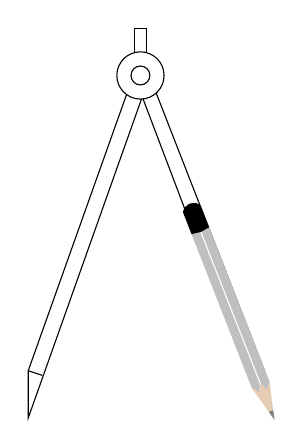
\begin{tikzpicture}
\begin{scope}[rotate=0,transform shape,scale=3]
\draw (2.95,3.7) rectangle (3,3.95);
\draw (2.92,3.68) -- (2.5,2.5) -- (2.5,2.3) -- (2.99,3.68);
\draw (3.5,2.5) -- (3.43,2.48) -- (2.975,3.68);
\draw (3.04,3.68) -- (3.5,2.5);
\draw (2.5,2.5) -- (2.56,2.48);
\draw[fill=white] (2.975,3.75) circle (0.1cm);
\draw (2.975,3.75) circle (0.04cm);
\end{scope}
\begin{scope}[xshift=10.34cm,yshift=7.28cm,rotate=21.4,scale=.6]          
\fill[gray!50] (0,4) -- (0.4,4) -- (0.4,0) --
               (0.3,-0.15) -- (0.2,0) -- (0.1,-0.14) --
               (0,0) -- cycle;
\draw[color=white] (0.2,4) -- (0.2,0);
\fill[black] (0,3.5) -- (0.2,3.47) -- (0.4,3.5) --
             (0.4,4) arc(30:150:0.23cm);
\fill[brown!40] (0,0) -- (0.2,-0.8)
    node[coordinate,pos=0.75](a){} -- 
    (0.4,0)node[coordinate,pos=0.25](b){} -- 
    (0.3,-0.15) -- (0.2,0) -- (0.1,-0.14) -- cycle;
\fill[gray] (a) -- (0.2,-0.8) -- (b) -- cycle;
\end{scope}
\end{tikzpicture}
\caption{Un compás  fijo. Un brazo tiene una aguja que se coloca en el centro del círculo. Un lápiz fijado al otro brazo sirve para dibujar el círculo. Los brazos están unidos por una bisagra ajustada modo que la distancia entre los brazos (el radio del círculo) se mantiene incluso cuando el compás se levanta del papel.}\label{fig.fixed-compass}
\end{minipage}
\hfill
\begin{minipage}{.45\textwidth}
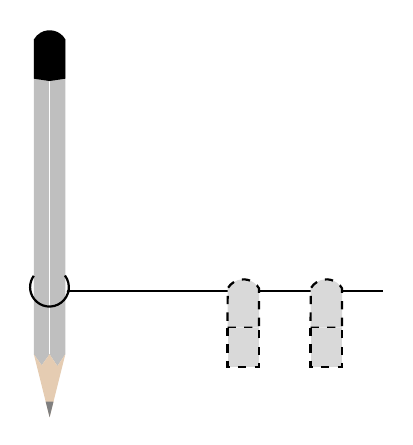
\begin{tikzpicture}[rotate=0,scale=1]          
\fill[gray!50] (0,4) -- (0.4,4) -- (0.4,0) --
               (0.3,-0.15) -- (0.2,0) -- (0.1,-0.14) --
               (0,0) -- cycle;
\draw[color=white] (0.2,4) -- (0.2,0);
\fill[black] (0,3.5) -- (0.2,3.47) -- (0.4,3.5) --
             (0.4,4) arc(30:150:0.23cm);
\fill[brown!40] (0,0) -- (0.2,-0.8)
    node[coordinate,pos=0.75](a){} -- 
    (0.4,0) node[coordinate,pos=0.25](b){} -- 
    (0.3,-0.15) -- (0.2,0) -- (0.1,-0.14) -- cycle;
\fill[gray] (a) -- (0.2,-0.8) -- (b) -- cycle;

\draw[thick] (0.395,1) arc (37:-216:7pt);
\coordinate (knot) at (0.44,.8);
\draw[thick] (knot) -- +(4,0);
\fill (knot) circle (.7pt);

\begin{scope}[xshift=100pt,yshift=-90pt]
\draw[dashed,thick,fill=white!70!gray] (0,3.5) -- (0.4,3.5) -- 
      (0.4,4) arc(30:150:0.23cm) -- cycle;
\draw[dashed,thick,fill=white!70!gray] (0,3.5) -- ++(0,-.5) -- ++(.4,0) -- ++(0,.5);
\end{scope}

\begin{scope}[xshift=70pt,yshift=-90pt]
\draw[dashed,thick,fill=white!70!gray] (0,3.5) -- (0.4,3.5) -- 
      (0.4,4) arc(30:150:0.23cm) -- cycle;
\draw[dashed,thick,fill=white!70!gray] (0,3.5) -- ++(0,-.5) -- ++(.4,0) -- ++(0,.5);
\end{scope}
\end{tikzpicture}
\caption{Un compás plegable. El usuario sujeta un trozo de cuerda en el centro del círculo. El otro extremo de la cuerda se ata a un lápiz y se utiliza para dibujar el círculo. Cuando se levanta el compás del papel, los dedos (punteados) pueden deslizarse fácilmente hasta una nueva posición.}\label{fig.collapsing-compass}
\end{minipage}
\end{figure}

Este capítulo comienza con una discusión sobre la relevancia de estudiar la construcción con regla y compás (Sec.~\ref{s.relevance}).
En el apartado~\ref{s.collapse} se comparan los dos tipos de compás en la construcción más elemental: una mediatriz. En el apartado~\ref{s.collapse-copy} se presenta el método de Euclides para copiar un segmento de recta utilizando un compás plegable. Esto demuestra que cualquier construcción que se pueda hacer usando un compás fijo se puede realizar usando un compás plegable. La sección~\ref{s.collapse-copy-incorrect} presenta una demostración de este teorema que parece correcta, pero no funciona para todas las configuraciones de rectas y puntos. Para enfatizar que no hay que fiarse de los diagramas, la sección~\ref{s.collapse-} presenta una famosa supuesta demostración de que todos los triángulos son ; la demostración parece correcta, pero no lo es porque se basa en un diagrama incorrecto.

\section{Construcción con regla y compás}\label{s.relevance}

La construcción con regla y compás solía ser el concepto fundamental que se enseñaba en geometría euclidiana. Recientemente, ha caído en desgracia en los programas escolares. Es cierto que el tema tiene poca o ninguna utilidad práctica. Como mostramos en las secciones~\ref{s.neusis}, \ref{s.neusis-doubling}, \ref{s.q}, \ref{s.square-quad}, los griegos sabían cómo realizar construcciones que son imposibles con una regla y un compás utilizando herramientas sólo ligeramente más avanzadas. Hoy en día, mediante métodos numéricos, los ordenadores pueden realizar construcciones con la precisión que se desee.

No obstante, creo que estudiar las construcciones tiene sus ventajas:
\begin{itemize}
\item Es más divertido y desafiante aprender geometría a través de construcciones que simplemente leyendo teoremas y demostraciones.
\item Se han logrado avances significativos en matemáticas mediante intentos de encontrar construcciones. El capítulo~\ref{c.heptadecagon} presenta una construcción de Gauss que condujo al álgebra abstracta moderna, en particular, la teoría desarrollada por \'{E}variste Galois.
\item Es algo contraintuitivo y por lo tanto muy interesante que se pueda demostrar que es imposible construir algunos objetos geométricos.
\item Lamentablemente, hay muchas personas que pierden años de su vida intentando realizar construcciones imposibles. Los estudiantes deberían ser conscientes de la inutilidad de tales esfuerzos.
\end{itemize}

\section{Compases fijos y compases plegables}\label{s.collapse}

Algunos libros de geometría presentan la construcción de la mediatriz de un segmento de recta construyendo dos circunferencias centradas en los extremos del segmento de forma que los radios sean iguales y mayores que la mitad de la longitud del segmento (Fig.~\ref{f.collapse-perp-bisector-fixed}). Esto sólo se puede hacer con un compás fijo porque después de dibujar el círculo centrado en $A$, la distancia entre los brazos del compás tiene que permanecer fija para dibujar el círculo centrado en $B$.

\begin{figure}[t]
\begin{minipage}{.45\textwidth}
\begin{center}
\begin{tikzpicture}[scale=0.5]
\coordinate (A) at (0,0);
\coordinate (B) at (4,0);
\vertex{A};
\vertex{B};
\draw (A) node[below left] {$A$} -- (B) node[below right] {$B$};
\draw[name path=larc] (A) ++(-60:3cm) arc (-60:60:3cm);
\draw[name path=rarc] (B) ++(-120:3cm) arc (-120:-240:3cm);
\path [name intersections={of=larc and rarc,by={b,t}}];
\node[above right,xshift=-2pt,yshift=5pt] at (t) {$C$};
\node[below left,xshift=2pt,yshift=-5pt] at (b) {$D$};
\draw ($ (b) ! 1.2 ! (t)$) -- ($ (t) ! 1.2 ! (b)$);
\end{tikzpicture}
\caption{Construcción de una mediatriz con compás fijo}\label{f.collapse-perp-bisector-fixed}
\end{center}
\end{minipage}
\hfill
\begin{minipage}{.45\textwidth}
\begin{center}
\begin{tikzpicture}[scale=0.5]
\coordinate (A) at (0,0);
\coordinate (B) at (4,0);
\vertex{A};
\vertex{B};
\draw (A) node[below left] {$A$} -- (B) node[below right] {$B$};
\draw[name path=larc] (A) ++(-80:4cm) arc (-80:80:4cm);
\draw[name path=rarc] (B) ++(-100:4cm) arc (-100:-260:4cm);
\path [name intersections={of=larc and rarc,by={b,t}}];
\node[above right,xshift=-2pt,yshift=3pt] at (t) {$C$};
\node[below left,xshift=2pt,yshift=-3pt] at (b) {$D$};
\draw ($ (b) ! 1.2 ! (t)$) -- ($ (t) ! 1.2 ! (b)$);
\end{tikzpicture}
\caption{Construcción de una mediatriz con compás fijo o plegable}\label{f.collapse-perp-bisector-collapse}
\end{center}
\end{minipage}
\end{figure}

Figura~\ref{f.collapse-perp-bisector-collapse} muestra la construcción de una mediatriz con compás fijo o con compás plegable. Se construyen dos circunferencias: una centrada en $A$ con radio $\overline{AB}$ y otra centrada en $B$ con radio $\overline{BA}$. Esto se puede hacer con un compás plegable porque (obviamente) $\overline{AB}=\overline{BA}$, por lo que el compás no tiene que ``recordar'' la longitud de $\overline{AB}$ para construir una circunferencia centrada en $B$ con el mismo radio.
La demostración de que la recta construida mostrada en la Fig.~\ref{f.collapse-perp-bisector-fixed} es una mediatriz no es nada elemental porque hay que utilizar conceptos relativamente avanzados como triángulos congruentes. Sin embargo, la demostración de que la construcción de una mediatriz mostrada en la Fig.~\ref{f.collapse-perp-bisector-collapse} es correcta es sencilla y se basa en el hecho de que $\triangle ABC$ es un triángulo equilátero. De hecho, esta es la primera proposición en los \textit{Elementos} de Euclides.
$\overline{AC}=\overline{AB}$ ya que son radios del mismo círculo, análogamente, $\overline{BC}=\overline{BA}$. Tenemos: $\overline{AC}=\overline{AB}=\overline{BA}=\overline{BC}$.

Figura~\ref{f.collapse-equilateral-fixed} muestra que para la construcción con compás fijo, el triángulo será un triángulo isósceles, no necesariamente equilátero (Fig.~\ref{f.collapse-equilateral-collapse}).

\section{Construcción de Euclides para copiar un segmento de recta}\label{s.collapse-copy}

La segunda proposición de los \textit{Elementos} de Euclides describe cómo copiar un segmento de recta $\overline{AB}$ dado un segmento de la misma longitud, uno de cuyos puntos extremos es un punto $C$ dado. Por lo tanto, un compás fijo no añade ninguna capacidad adicional y basta con un compás plegable, aunque las construcciones son más fáciles con un compás fijo.

\begin{theorem}
Dado un segmento de recta $\overline{AB}$ y un punto $C$, se puede construir un segmento de recta $\overline{CC'}$, uno de cuyos puntos extremos es $C$, utilizando un compás plegable, tal que $\overline{AB}=\overline{CC'}$ (Fig.~\ref{f.collapse-copying-1}).
\end{theorem}

\begin{figure}[t]
\begin{minipage}{.45\textwidth}
\begin{center}
\begin{tikzpicture}[scale=0.5]
\coordinate (A) at (0,0);
\coordinate (B) at (4,0);
\vertex{A};
\vertex{B};
\draw (A) node[below left] {$A$} -- (B) node[below right] {$B$};
\draw[name path=larc] (A) ++(-60:3cm) arc (-60:60:3cm);
\draw[name path=rarc] (B) ++(-120:3cm) arc (-120:-240:3cm);
\path [name intersections={of=larc and rarc,by={b,t}}];
\vertex{t};
\vertex{b};
\node[above right,xshift=-2pt,yshift=5pt] at (t) {$C$};
\node[below left,xshift=2pt,yshift=-5pt] at (b) {$D$};
\draw (A) -- (t);
\draw (B) -- (t);
\end{tikzpicture}
\caption{Construcción de un triángulo isóceles con compás fijo}\label{f.collapse-equilateral-fixed}
\end{center}
\end{minipage}
\hfill
\begin{minipage}{.45\textwidth}
\begin{center}
\begin{tikzpicture}[scale=0.5]
\coordinate (A) at (0,0);
\coordinate (B) at (4,0);
\draw (A) node[below left] {$A$} -- (B) node[below right] {$B$};
\vertex{A};
\vertex{B};
\draw[name path=larc] (A) ++(-80:4cm) arc (-80:80:4cm);
\draw[name path=rarc] (B) ++(-100:4cm) arc (-100:-260:4cm);
\path [name intersections={of=larc and rarc,by={b,t}}];
\vertex{t};
\vertex{b};
\node[above right,xshift=-2pt,yshift=3pt] at (t) {$C$};
\node[below left,xshift=2pt,yshift=-3pt] at (b) {$D$};
\draw (A) -- (t);
\draw (B) -- (t);
\end{tikzpicture}
\caption{Construcción de un triángulo equilátero con un compás plegable}\label{f.collapse-equilateral-collapse}
\end{center}
\end{minipage}
\end{figure}

\begin{figure}[b]
\begin{minipage}{.45\textwidth}
\begin{center}
\begin{tikzpicture}[scale=0.5]
\coordinate (C) at (0,0);
\coordinate (A) at (3,0);
\draw (A) node[below,xshift=-2pt,yshift=-2pt] {$A$} -- +(40:4) coordinate (B) node[right] {$B$};
\vertex{A};
\vertex{B};
\vertex{C};
\node[below,xshift=2pt,yshift=-2pt] at (C) {$C$};
\draw[thick,dashed] (C) -- +(160:4) coordinate (D) node[below] {$C'$};
\vertex{D};
\end{tikzpicture}
\caption{Copiar el segmento de recta $\overline{AB}$. La orientación de $\overline{CC'}$ no es importante.}\label{f.collapse-copying-1}
\end{center}
\end{minipage}
\hfill
\begin{minipage}{.45\textwidth}
\begin{center}
\begin{tikzpicture}[scale=0.5]
\coordinate (C) at (0,0);
\coordinate (A) at (3,0);
\draw (A) node[below,xshift=-2pt,yshift=-2pt] {$A$} -- +(40:4) coordinate (B) node[right] {$B$};
\vertex{B};
\node[below,xshift=2pt,yshift=-2pt] at (C) {$C$};
\draw (A) -- (C);
\path[name path=larc] (C) ++(-70:2.5cm) arc (-70:70:2.5cm);
\path[name path=rarc] (A) ++(-110:2.5cm) arc (-110:-250:2.5cm);
\path [name intersections={of=larc and rarc,by={d,D}}];
\node[above] at (D) {$D$};
\draw (A) -- (D);
\draw (C) -- (D);
\end{tikzpicture}
\caption{Copiar un segmento de línea con un compás plegable}\label{f.collapse-copying-2}
\end{center}
\end{minipage}
\end{figure}

\begin{proof}
Construimos el segmento de recta $\overline{AC}$. Construimos el triángulo equilátero $\triangle ACD$ cuya base es $\overline{AC}$ (Fig.~\ref{f.collapse-copying-2}). Por la primera proposición de Euclides, el triángulo se puede construir utilizando un compás plegable. Construimos la semirrecta que es prolongación del segmento \emph{de $D$ a $A$}, y construir la semirrecta que es prolongación de la recta segmento \emph{de $D$ a $C$} (Fig.~\ref{f.collapse-copying-3}). Construimos la circunferencia centrada en $A$ con radio $\overline{AB}$ y denotamos con E la intersección de la circunferencia y la semirrecta que prolonga $\overline{DA}$ (Fig.~\ref{f.collapse-copying-4}). Construimos la circunferencia centrada en $D$ con radio $\overline{DE}$ y denotamos con $F$ la intersección de la circunferencia y la semirrecta que prolonga $\overline{DC}$ (Fig.~\ref{f.collapse-copying-5}).

\begin{figure}[t]
\begin{minipage}{.45\textwidth}
\begin{center}
\begin{tikzpicture}[scale=0.4]
\coordinate (C) at (0,0);
\coordinate (A) at (3,0);
\draw (A) node[below,xshift=-2pt,yshift=-2pt] {$A$} -- +(40:4) coordinate (B) node[right] {$B$};
\node[below,xshift=2pt,yshift=-2pt] at (C) {$C$};
\draw (A) -- (C);
\path[name path=larc] (C) ++(-70:2.5cm) arc (-70:70:2.5cm);
\path[name path=rarc] (A) ++(-110:2.5cm) arc (-110:-250:2.5cm);
\path [name intersections={of=larc and rarc,by={d,D}}];
\node[above] at (D) {$D$};
\draw (A) -- (D);
\draw (C) -- (D);
\draw[name path=ray2] (D) -- ($ (D) ! 3 ! (C) $);
\draw[name path=ray1] (D) -- ($ (D) ! 3 ! (A) $);
\end{tikzpicture}
\caption{Construcción de semirrectas a partir de $D$}\label{f.collapse-copying-3}
\end{center}
\end{minipage}
\hfill
\begin{minipage}{.45\textwidth}
\begin{center}
\begin{tikzpicture}[scale=0.4]
\coordinate (C) at (0,0);
\coordinate (A) at (3,0);
\draw (A) node[below,xshift=-2pt,yshift=-2pt] {$A$} -- +(40:4) coordinate (B) node[right] {$B$};
\node[below,xshift=2pt,yshift=-2pt] at (C) {$C$};
\draw (A) -- (C);
\path[name path=larc] (C) ++(-70:2.5cm) arc (-70:70:2.5cm);
\path[name path=rarc] (A) ++(-110:2.5cm) arc (-110:-250:2.5cm);
\path [name intersections={of=larc and rarc,by={d,D}}];
\node[above] at (D) {$D$};
\draw (A) -- (D);
\draw (C) -- (D);
\draw[name path=ray2] (D) -- ($ (D) ! 3 ! (C) $);
\draw[name path=ray1] (D) -- ($ (D) ! 3 ! (A) $);
\node[draw,circle through=(B),name path=c1] at (A) {};
\path [name intersections={of=c1 and ray1,by={E,e}}];
\node[right,xshift=2pt,yshift=-2pt] at (E) {$E$};
\end{tikzpicture}
\caption{Construimos un círculo de radio $\overline{AB}$}\label{f.collapse-copying-4}
\end{center}
\end{minipage}
\end{figure}

$\overline{DC}=\overline{DA}$ porque el $\triangle ACD$ es equilátero. $\overline{AE}=\overline{AB}$ son radios de lamisma circunferencia, al igual que $\overline{DF}=\overline{DE}$. Por lo tanto:
\[
\overline{CF}=\overline{DF}-\overline{DC}=\overline{DE}-\overline{DC}=\overline{DE}-\overline{DA}=\overline{AE}=\overline{AB}\,.
\]
\end{proof}

\begin{figure}[b]
\begin{center}
\begin{tikzpicture}[scale=0.4]
\clip (-5,-4.5) rectangle (8,6);
\coordinate (C) at (0,0);
\coordinate (A) at (3,0);
\draw (A) node[below,xshift=-2pt,yshift=-2pt] {$A$} -- +(40:4) coordinate (B) node[right] {$B$};
\node[below,xshift=2pt,yshift=-2pt] at (C) {$C$};
\draw (A) -- (C);
\path[name path=larc] (C) ++(-70:2.5cm) arc (-70:70:2.5cm);
\path[name path=rarc] (A) ++(-110:2.5cm) arc (-110:-250:2.5cm);
\path [name intersections={of=larc and rarc,by={d,D}}];
\node[above] at (D) {$D$};
\draw (A) -- (D);
\draw (C) -- (D);
\draw[name path=ray2] (D) -- ($ (D) ! 3 ! (C) $);
\draw[name path=ray1] (D) -- ($ (D) ! 3 ! (A) $);
\node[draw,circle through=(B),name path=c1] at (A) {};
\path [name intersections={of=c1 and ray1,by={E,e}}];
\node[right,xshift=2pt,yshift=-2pt] at (E) {$E$};
\node[draw,circle through=(E),name path=c2] at (D) {};
\path [name intersections={of=c2 and ray2,by={F,f}}];
\node[left,xshift=-2pt,yshift=-2pt] at (F) {$F$};
\path (A) -- node[right] {$a$} (E);
\path (C) -- node[left] {$a$} (F);
\draw[white,fill=white] (-5,4.5) rectangle +(13,1.5);
\end{tikzpicture}
\end{center}
\caption{Construcción de $\overline{CF}=\overline{AB}$}\label{f.collapse-copying-5}
\end{figure}

La especificación de las direcciones de las semirrectas es esencial. La demostración funciona para cualquier segmento de recta $\overline{AB}$ y cualquier punto $C$, independientemente de su posición respecto a $\overline{AB}$.  Especificando las direcciones, el ``cono'' encerrado por los dos rayos intersecará los círculos aunque $\overline{AC}>\overline{AB}$ (Fig.~\ref{f.collapse-copying-6}).

\begin{figure}
\begin{center}
\begin{tikzpicture}[scale=0.4]
\clip (-12,-6) rectangle (11,10);
\coordinate (C) at (-4,0);
\coordinate (A) at (3,0);
\draw (A) node[below,xshift=-2pt,yshift=-2pt] {$A$} -- +(40:4) coordinate (B) node[right] {$B$};
\node[below,xshift=2pt,yshift=-2pt] at (C) {$C$};
\draw (A) -- (C);
\path[name path=larc] (C) ++(-70:7cm) arc (-70:70:7cm);
\path[name path=rarc] (A) ++(-110:7cm) arc (-110:-250:7cm);
\path [name intersections={of=larc and rarc,by={d,D}}];
\node[above] at (D) {$D$};
\draw (A) -- (D);
\draw (C) -- (D);
\draw[name path=ray2] (D) -- ($ (D) ! 2 ! (C) $);
\draw[name path=ray1] (D) -- ($ (D) ! 2 ! (A) $);
\node[draw,circle through=(B),name path=c1] at (A) {};
\path [name intersections={of=c1 and ray1,by={e,E}}];
\node[right,xshift=2pt,yshift=-2pt] at (E) {$E$};
\node[draw,circle through=(E),name path=c2] at (D) {};
\path [name intersections={of=c2 and ray2,by={F,f}}];
\node[left,xshift=-2pt,yshift=-2pt] at (F) {$F$};
\path (A) -- node[right] {$a$} (E);
\path (C) -- node[left] {$a$} (F);
\draw[white,fill=white] (-12,8) rectangle +(23,2);
\end{tikzpicture}
\end{center}
\caption{Construcción para $\overline{AC}>\overline{AB}$}\label{f.collapse-copying-6}
\end{figure}

%%%%%%%%%%%%%%%%%%%%%%%%%%%%%%%%%%%%%%%%%%%%%%%%%%%%%%%%%%%%%%%

\section{Una construcción errónea para copiar un segmento de línea}\label{s.collapse-copy-incorrect}

\begin{proof}
Construimos tres circunferencias: una centrada en $A$ con radio $\overline{AB}$, otra centrada en $A$ con radio $\overline{AC}$, y otra centrada en $C$ con radio $\overline{AC}=\overline{CA}$. Denotamos las intersecciones de las circunferencias centradas en $A$ y $C$ con $E$ y $F$, respectivamente, y denotamos una intersección de la circunferencia centrada en $C$ y la circunferencia centrada en $A$ con radio $\overline{AB}$ con $D$. Si $\overline{AC}>\overline{AB}$, la construcción es como se muestra en Fig.~\ref{f.collapse-incorrect-1}.
\begin{figure}[b]
\begin{center}
\begin{tikzpicture}[scale=0.5]
\coordinate (C) at (-2,0);
\coordinate (A) at (2.5,0);
\coordinate (B) at (4.5,1.5);
\draw (A) node[below right] {$A$} -- (B) node[right] {$B$};
\node[left,xshift=-2pt] at (C) {$C$};
\node[draw,circle through=(B),name path=c1] at (A) {};
\node[draw,circle through=(C),name path=c2] at (A) {};
\node[draw,circle through=(A),name path=c3] at (C) {};
\path [name intersections={of=c1 and c3,by={D,f}}];
\path [name intersections={of=c2 and c3,by={E,F}}];
\node[below right,xshift=4pt] at (D) {$D$};
\node[above,yshift=2pt] at (E) {$E$};
\node[below,yshift=-2pt] at (F) {$F$};
\vertex{C};
\end{tikzpicture}
\end{center}
\caption{Construcción para copiar un segmento de recta (1)}\label{f.collapse-incorrect-1}
\end{figure}

\begin{figure}[t]
\begin{center}
\begin{tikzpicture}[scale=0.5]
\clip (-8,-1) rectangle (9,5);
\coordinate (C) at (-2,0);
\coordinate (A) at (2.5,0);
\coordinate (B) at (4.5,1.5);
\draw[thick] (A) node[below right] {$A$} -- (B) node[right] {$B$};
\vertex{A};
\vertex{C};
\node[below left] at (C) {$C$};
\node[draw,circle through=(B),name path=c1] at (A) {};
\node[draw,circle through=(C),name path=c2] at (A) {};
\node[draw,circle through=(A),name path=c3] at (C) {};
\path [name intersections={of=c1 and c3,by={D,f}}];
\path [name intersections={of=c2 and c3,by={E,F}}];
\node[draw,circle through=(D),name path=c4] at (E) {};
\path [name intersections={of=c2 and c4,by={g,G}}];
\node[left] at (G) {$G$};
\node[below right,yshift=2pt,xshift=2pt] at (D) {$D$};
\node[above] at (E) {$E$};
\vertex{E};
\vertex{F};
\draw (C) -- (G);
\draw (A) -- (G) -- (E) -- (C) -- (D);
\draw (A) -- (D) -- (E) -- cycle;
\end{tikzpicture}
\end{center}
\caption{Construcción para copiar un segmento de recta (2)}\label{f.collapse-incorrect-2}
\end{figure}

Construimos una circunferencia centrada en $E$ con radio $\overline{ED}$. Denotemos por $G$ la intersección de esta circunferencia con la circunferencia centrada en $A$ de radio $\overline{AC}$. Hay dos intersecciones, por lo que elegir la más cercana a $C$ (Fig.~\ref{f.collapse-incorrect-2}).
$\overline{CD}=\overline{CE}$ son radios de la misma circunferencia que $\overline{AE}=\overline{AG}$. Por construcción los radios $\overline{CE}$ y $\overline{AE}$ son iguales. Por tanto:
\[
\overline{CD} = \overline{CE} = \overline{AE} = \overline{AG}\,.
\]
$\overline{EG} = \overline{ED}$ son radios del mismo círculo, por lo que $\triangle EAG\cong \triangle DCE$ por lado-lado-lado y $\angle GEA = \angle DEC$.

Como:
\[
\angle GEC = \angle GEA \!-\!\angle CEA = \angle DEC\!-\!\angle CEA = \angle DEA\,,
\]
resulta que $\triangle ADE\cong\triangle CGE$ por lado-ángulo-lado. $\overline{AB}=\overline{AD}$ son radios del círculo menor centrado en $A$, por lo que $\overline{GC}=\overline{AD}=\overline{AB}$.
\end{proof}

La demostración sólo es correcta si $\overline{AC}>\overline{AB}$.  Figura~\ref{f.collapse-incorrect-4} muestra un diagrama donde $\overline{AC}<\overline{AB}$ y se puede ver que $\overline{AB}\neq\overline{GC}$.

\begin{figure}[b]
\begin{center}
\begin{tikzpicture}[scale=0.5]
\coordinate (C) at (-1,0);
\coordinate (A) at (2,0);
\coordinate (B) at (6,1.5);
\draw[thick] (A) node[below right] {$A$} -- (B) node[right] {$B$};
\node[left,xshift=-2pt] at (C) {$C$};
\node[draw,circle through=(B),name path=c1] at (A) {};
\node[draw,circle through=(C),name path=c2] at (A) {};
\node[draw,circle through=(A),name path=c3] at (C) {};
\path [name intersections={of=c1 and c3,by={D,f}}];
\path [name intersections={of=c2 and c3,by={E,F}}];
\node[above left,xshift=4pt] at (D) {$D$};
\node[above,yshift=2pt] at (E) {$E$};
\node[below,yshift=-2pt] at (F) {$F$};
\vertex{A};
\vertex{C};
\node[draw,circle through=(D),name path=c4] at (E) {};
\path [name intersections={of=c2 and c4,by={g,G}}];
\node[right,xshift=2pt,yshift=2pt] at (G) {$G$};
\draw[thick] (G) -- (C);
\end{tikzpicture}
\end{center}
\caption{Un diagrama para el que la demostración no funciona}\label{f.collapse-incorrect-4}
\end{figure}


\section{No te fíes de un diagrama}\label{s.collapse-}

\begin{theorem}[Incorrecto, por supuesto]
Todos los triángulos son isósceles.
\end{theorem}\index{Triangle!@all are }

\begin{proof}
Dado un triángulo arbitrario $\triangle ABC$, sea $P$ la intersección de la bisectriz del ángulo $\angle BAC$ y la mediatriz de $\overline{BC}$. Las intersecciones de las altitudes desde $P$ a los lados $\overline{AB}$, $\overline{AC}$ se denotan por $E,F$, respectivamente (Fig.~\ref{f.collapse--1}). 
\begin{figure}[t]
\begin{center}
\begin{tikzpicture}[scale=1]
\coordinate (P) at (0,0);
\node[xshift=4mm,yshift=1mm] at (P) {$P$};
\coordinate [label=left:$B$] (B)  at (-2,-2);
\coordinate [label=right:$C$] (C)  at (4,-2);
\coordinate [label=above:$A$] (A)  at (-1,2);
\node[below,yshift=-12pt,xshift=1pt] at (A) {$\alpha$};
\node[below,yshift=-12pt,xshift=13pt] at (A) {$\alpha$};
\draw (A) -- (B);
\draw (A) -- (C);
\draw (B) -- (C);
\draw (A) -- (P);
\draw (B) -- (P);
\draw (C) -- (P);
\coordinate[label=left:$E$] (E) at ($ (A) ! .44 ! (B) $);
\draw[rotate=-100] (E) rectangle +(6pt,6pt);
\draw (P) -- (E);
\coordinate (F) at ($ (A) ! .33 ! (C) $);
\node[right,xshift=2pt,yshift=2pt] at (F) {$F$};
\draw[rotate=-132] (F) rectangle +(6pt,6pt);
\draw (P) -- (F);
\coordinate[label=below:$D$] (D) at ($ (B) ! .33 ! (C) $);
\draw (D) rectangle +(6pt,6pt);
\draw (P) -- (D);
\node[left] at ($ (A) ! .5 ! (E) $) {};
\node[left] at ($ (B) ! .5 ! (E) $) {};
\node[below] at ($ (B) ! .5 ! (D) $) {$a$};
\node[below] at ($ (C) ! .5 ! (D) $) {$a$};
\node[right,xshift=2pt] at ($ (A) ! .5 ! (F) $) {};
\node[right,xshift=2pt] at ($ (C) ! .5 ! (F) $) {};
\vertex{P};
\end{tikzpicture}
\end{center}
\caption{Una demostración incorrecta de que todos los triángulos son isóceles}\label{f.collapse--1}
\end{figure}
$\triangle APE\cong \triangle APF$ porque son triángulos rectángulos con ángulos iguales $\alpha$ y lado común $\overline{AP}$. $\triangle DPB\cong \triangle DPC$ ya que son triángulos rectángulos, $\overline{PD}$ es un lado común y $\overline{BD}=\overline{CD}=a$. $\triangle EPB\cong \triangle FPC$ ya que son triángulos rectángulos, $\overline{EP}=\overline{PF}$ por la primera congruencia y $\overline{PB}=\overline{PC}$ por la segunda congruencia. Combinando las ecuaciones obtenemos que $\triangle ABC$ es :
\[
\overline{AB}= \overline{AE}+\overline{EB}=\overline{AF}+\overline{FC} =\overline{AC}\,.
\]
\end{proof}

La lógica de la demostración es correcta, pero el diagrama en el que se basa la demostración no es correcto porque el punto $P$ está fuera del triángulo. (Fig.~\ref{f.collapse--2}).

\begin{figure}[b]
\begin{center}
\begin{tikzpicture}[scale=.5]
\coordinate (B) at (0,0);
\coordinate (C) at (8,0);
\path[name path=ba] (B) -- +(70:6);
\path[name path=ca] (C) -- +(140:8.5);
\path [name intersections={of=ba and ca,by={A}}];
\draw (B) -- (C) -- (A) -- cycle;
\node[above] at (A) {$A$};
\node[below,yshift=-12pt,xshift=-1pt] at (A) {$\alpha$};
\node[below right,xshift=5pt,yshift=-12pt] at (A) {$\alpha$};
\node[left] at (B) {$B$};
\node[right] at (C) {$C$};
\draw[name path=angle] (A) -- +(-75:9);
\draw ($(B)!.5!(C)$) -- +(0,3);
\draw[name path=perp] ($(B)!.5!(C)$) -- +(0,-3.5);
\path [name intersections={of=angle and perp,by={X}}];
\vertex{X};
\draw (4,0) rectangle +(10pt,10pt);
\node[right] at (X) {$P$};
\end{tikzpicture}
\caption{Por qué no funciona la construcción}\label{f.collapse--2}
\end{center}
\end{figure}

\subsection*{¿Cuál es la sorpresa?}

De estudiante daba por sentado que un compás tiene una bisagra que mantiene la distancia entre la punta y el lápiz cuando se levanta del papel. Cuando el profesor utilizaba un compás hecho con un trozo de cuerda y un trozo de tiza, nunca imaginé que se diferenciara de mi compás. El artículo de Gotfried Toussaint fue una verdadera sorpresa, al igual que su demostración de que las demostraciones posteriores a Euclides eran incorrectas porque dependían de diagramas que hacían suposiciones injustificadas. Recomiendo el artículo a los lectores que deseen profundizar en el conocimiento de las demostraciones en matemáticas.

\subsection*{Fuentes}

Este capítulo se basa en \cite{toussaint}. La construcción incorrecta de la equivalencia de los dos compases en Sect.~\ref{s.collapse-copy-incorrect} es de \cite{rusty}. Thomas L. Heath, uno de los mayores expertos en matemáticas griegas, ha escrito una exhaustiva traducción al inglés de los \textit{Elements} de Euclides junto con un extenso comentario \cite{euclid}.


\tikzsetfigurename{trisect-an-angle}
\include{trisect-an-angle}

\tikzsetfigurename{square-a-circle}
\include{square-a-circle}

%%%%%%%%%%%%%%%%%%%  Coloring

\tikzsetfigurename{five-color}
\include{five-color}

\tikzsetfigurename{museum}
% !TeX root = surprises.tex

\selectlanguage{hebrew}



\chapter{איך לשמור על מוזיאון}
\label{c.museum}

ב-%
$1973$
\L{Victor Klee}
שאל כמה שומרים נחוצים כדי לראות את כל הקירות של מוזיאון על מנת לוודא שלא גונבים את הציורים. אם הקירות של המוזיאון מהווים מצולע משוכלל או אפילו מצולע קמור, אפשר להסתפק בשומר אחד:
\begin{center}

\begin{tikzpicture}[scale=.8]
\coordinate (O) at (0,0);
\fill (O) circle (2pt);
\foreach \x/\name/\n/\po in {0/a/A/right,.6/b/B/above,1.6/c/C/left,2.4/d/D/below left,3.9/e/E/below right} {
  \coordinate (\name) at ($(O)+(\x*72+18:3cm)$);
%  \fill (\name) circle (1.5pt);
%  \node[\po] at (\name) {$\n$};
\draw[dashed] (O) -- (\name);
}
\draw (a) -- (b) -- (c) -- (d) --(e) -- cycle;
\end{tikzpicture}
\end{center}

מה עם מוזיאון עם קירות בצורה של מסור:

\begin{center}

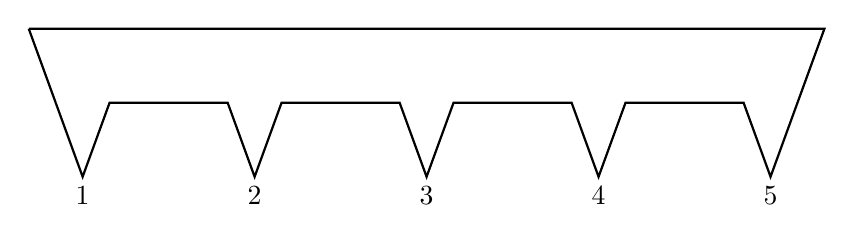
\begin{tikzpicture}[scale=1]
\coordinate (O) at (0,0);
\draw [thick] (O) -- (++110:1cm) coordinate (P);
\draw[thick] (O) --
  ++(-70:1cm) coordinate(A) node[below] {$1$} -- 
  ++(+70:1cm) -- ++(0:1.5cm) --
  ++(-70:1cm) coordinate(B) node[below] {$2$} -- 
  ++(+70:1cm) -- ++(0:1.5cm) --
  ++(-70:1cm) coordinate(C) node[below] {$3$}-- 
  ++(+70:1cm) -- ++(0:1.5cm) --
  ++(-70:1cm) coordinate(D) node[below] {$4$} -- 
  ++(+70:1cm) -- ++(0:1.5cm) --
  ++(-70:1cm) coordinate(E) node[below] {$5$} --
  ++(+70:2cm) -- (P);

\end{tikzpicture}
\end{center}

וודא על ידי ספירה שיש 
$15$
קירות.

כל "שן" של המסור מגדירה משולש )מסומן באפור(. שומרת הניצבת במקום כלשהו בתוך אחד המשולשים יכולה לראות את כל הקירות של אותו משולש:

\begin{center}

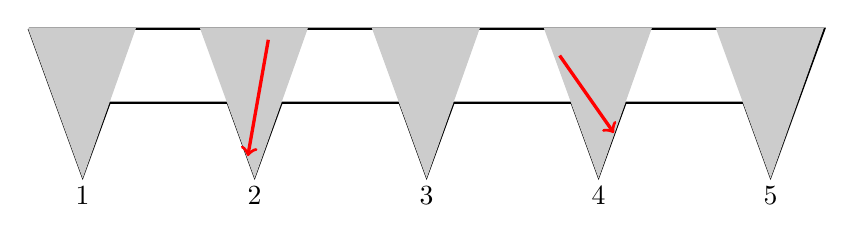
\begin{tikzpicture}[scale=1]
\coordinate (O) at (0,0);
\draw [thick] (O) -- (++110:1cm) coordinate (P);
\draw[thick] (O) --
  ++(-70:1cm) coordinate(A) node[below] {$1$} -- 
  ++(+70:1cm) -- ++(0:1.5cm) --
  ++(-70:1cm) coordinate(B) node[below] {$2$} -- 
  ++(+70:1cm) -- ++(0:1.5cm) --
  ++(-70:1cm) coordinate(C) node[below] {$3$}-- 
  ++(+70:1cm) -- ++(0:1.5cm) --
  ++(-70:1cm) coordinate(D) node[below] {$4$} -- 
  ++(+70:1cm) -- ++(0:1.5cm) --
  ++(-70:1cm) coordinate(E) node[below] {$5$} --
  ++(+70:2cm) -- (P);

\draw[fill,black!20!white] (A) -- ++(110:2cm) -- ++(0:1.35cm)-- cycle;
\draw[fill,black!20!white] (B) -- ++(110:2cm) -- ++(0:1.35cm)-- cycle;
\draw[fill,black!20!white] (C) -- ++(110:2cm) -- ++(0:1.35cm)-- cycle;
\draw[fill,black!20!white] (D) -- ++(110:2cm) -- ++(0:1.35cm)-- cycle;
\draw[fill,black!20!white] (E) -- ++(110:2cm) -- ++(0:1.35cm)-- cycle;

\draw[->,red,very thick] (2.7,.8) -- +(-100:1.5cm);
\draw[->,red,very thick] (6.4,.6) -- +(-55:1.2cm);
%\draw[->,very thick,green] (9,.9) -- (C);
%\draw[->,very thick,blue] ($(O)+(.5,.5)$) -- ++(7.5,.42);
%\draw[->,very thick,blue] ($(O)+(.5,.5)$) -- ++(3,-.5);
\end{tikzpicture}
\end{center}

אם השומרת ניצבת בקירבת הקיר העליון היא יכולה לראות את כל הקירות האופקיים )חצים כחולים(. ברור שחמש
שומרות מספיקות כדי לשמור על כל הקירות. אם המשולשים לא חופפים, שומרת במשולש אחד לא יכולה לראות את כל הקירות של משולש אחר )חץ ירוק(, לכן חייבים להעסיק חמש שומרות נחוצות.

\begin{center}

\begin{tikzpicture}[scale=1]
\coordinate (O) at (0,0);
\draw [thick] (O) -- (++110:1cm) coordinate (P);
\draw[thick] (O) --
  ++(-70:1cm) coordinate(A) node[below] {$1$} -- 
  ++(+70:1cm) -- ++(0:1.5cm) --
  ++(-70:1cm) coordinate(B) node[below] {$2$} -- 
  ++(+70:1cm) -- ++(0:1.5cm) --
  ++(-70:1cm) coordinate(C) node[below] {$3$}-- 
  ++(+70:1cm) -- ++(0:1.5cm) --
  ++(-70:1cm) coordinate(D) node[below] {$4$} -- 
  ++(+70:1cm) -- ++(0:1.5cm) --
  ++(-70:1cm) coordinate(E) node[below] {$5$} --
  ++(+70:2cm) -- (P);

\draw[fill,black!20!white] (A) -- ++(110:2cm) -- ++(0:1.35cm)-- cycle;
\draw[fill,black!20!white] (B) -- ++(110:2cm) -- ++(0:1.35cm)-- cycle;
\draw[fill,black!20!white] (C) -- ++(110:2cm) -- ++(0:1.35cm)-- cycle;
\draw[fill,black!20!white] (D) -- ++(110:2cm) -- ++(0:1.35cm)-- cycle;
\draw[fill,black!20!white] (E) -- ++(110:2cm) -- ++(0:1.35cm)-- cycle;

%\draw[->,red,very thick] (2.7,1) -- (B);
\draw[->,very thick,green,dashed] (9,.8) -- +(-165:4.6cm);
\draw[->,very thick,blue] ($(O)+(.5,.5)$) -- ++(7.4,.4);
\draw[->,very thick,blue] ($(O)+(.5,.5)$) -- ++(2.9,-.45);
\draw (6,0) circle(4pt);
\draw (4.95,-.28) circle(4pt);
\end{tikzpicture}
\end{center}
\begin{theorem}\label{thm.guarded} \mbox{}\\
$\disfrac{n}{3}$
שומרות מספיקות ונחוצות כדי לשמור על כל מוזיאון עם
$n$
קירות.%
\footnote{\R{אם}
$n$
\R{לא מתחלק ב}-%
$3$
\R{מספר השומרות הנחוצות הוא}
$\left\lfloor \disfrac{n}{3}\right\rfloor$.
\R{למשל,}
$4$
\R{שומרות מספיקות כדי לשמור על מוזיאונים עם}
$12, 13, 14$
\R{קירות כי}
$\left\lfloor \disfrac{14}{3}\right\rfloor =\left\lfloor \disfrac{13}{3}\right\rfloor=\left\lfloor \disfrac{12}{3}\right\rfloor=4$.
\R{לשם הפשטות נתעלם מסיבוך זה}.}
\end{theorem}
ניתן להכליל את הדוגמה כדי להראות ש-%
$\disfrac{n}{3}$
שומרות נחוצות. שאר הפרק מוקדש להוכחה ש-%
$\disfrac{n}{3}$
מספיקות עבור כל מוזיאון.

\section{צביעת מצולעים מתולתים}

\textbf{הגדרה:}
קודקוד במצולע הוא 
\textbf{קמור}
אם הזווית הפנימית פחות מ-%
$180^\circ$.
קודקוד במצולע הוא
\textbf{קעור}
אם הזווית הפנימית גדולה מ-%
$180^\circ$.

במצולע באיור להלן, קודקוד 
$1$
קמור וקודקוד
$2$
קעור.
\begin{center}

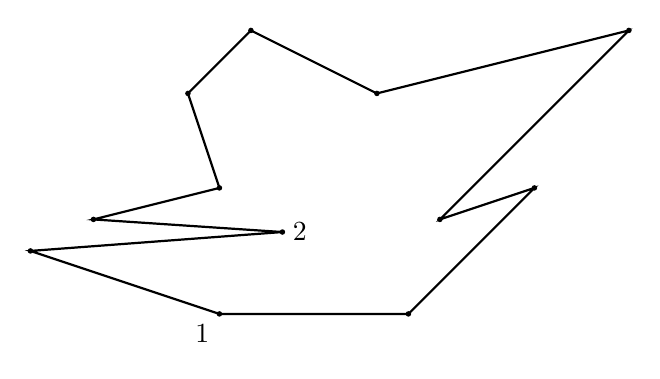
\begin{tikzpicture}[scale=.8]
\draw[thick]
  (0,0) coordinate (A) node[below left] {$1$} -- 
  ++(3,0) coordinate (B) --
  ++(2,2) coordinate (C) --
  ++(-1.5,-.5) coordinate (D) --
  ++(3,3) coordinate (E) -- 
  ++(-4,-1) coordinate (F) --
  ++(-2,1) coordinate (G) --
  ++(-1,-1) coordinate (H) --
  ++(.5,-1.5) coordinate (I) --
  ++(-2,-.5) coordinate (J) --
  ++(3,-.2) coordinate (K) node[right] {$2$} -- 
  ++(-4,-.3) coordinate (L) --
  cycle;
  
\foreach \point in {A,B,C,D,E,F,G,H,I,J,K,L}
  \fill (\point) circle(1.25pt);
\end{tikzpicture}
\end{center}
\textbf{הגדרה:}
ניתן
\textbf{לתלת}
\L{(triangulate)}
מצולע אם ניתן לצייר 
\textbf{אלכסונים},
קטעי קו שאינם נחתכים המחברים קודקודים והנמצאים בתוך המצולע לכל אורכם, כך שהשטח הפנימי של המצולע מכוסה על ידי משולשים זרים אחד מהשני.



\begin{theorem}\label{thm.tri}\mbox{}\\
ניתן לתלת כל מצולע.
\end{theorem}
אנו דוחים את ההוכחה של משפט~%
\ref{thm.tri}
לשלב מאוחר יותר.
\textbf{הגדרה:}
ניתן
\textbf{לצבוע מצולע בשלושה צבעים}
אם קיים מיפוי
\[
c: V \mapsto \{\textrm{\R{אדום, כחול, ירוק}}\}
\]
כך ששני הקודקודים של צלע מקבלים צבעים שונים.
\begin{theorem}\mbox{}\\
ניתן לצבוע מצולע מתולת בשלושה צבעים.
\label{thm.colored}
\end{theorem}
\textbf{הוכחה:}
באינדוקציה על מספר הקודקודים. ברור שניתן לצבוע משולש בשלושה צבעים. ניתן מצולע עם 
$n>3$
קודקודים. חייבים לצייר לפחות אלכסון אחד כדי לתלת את המצולע. בחר אלכסון שרירותי
$\overline{AB}$:

\begin{center}

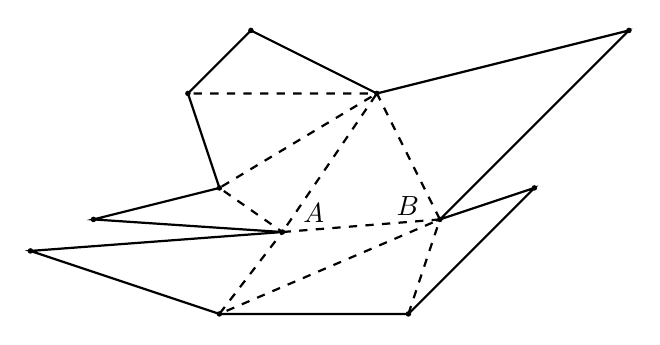
\begin{tikzpicture}[scale=.8]
\draw[thick]
  (0,0) coordinate (A) -- 
  ++(3,0) coordinate (B) --
  ++(2,2) coordinate (C) --
  ++(-1.5,-.5) coordinate (D) --
  ++(3,3) coordinate (E) -- 
  ++(-4,-1) coordinate (F) --
  ++(-2,1) coordinate (G) --
  ++(-1,-1) coordinate (H) --
  ++(.5,-1.5) coordinate (I) --
  ++(-2,-.5) coordinate (J) --
  ++(3,-.2) coordinate (K) -- 
  ++(-4,-.3) coordinate (L) --
  cycle;
  
\foreach \point in {A,B,C,D,E,F,G,H,I,J,K,L}
  \fill (\point) circle(1.25pt);

\node[above right,xshift=4pt] at (K) {$A$};
\node[above left,xshift=-4pt,yshift=-2pt] at (D) {$B$};

\draw[thick,dashed]
  (B) -- (D) -- (K) -- (F) -- (I) -- (K) -- (A) -- (D) -- (F) -- (H);
\end{tikzpicture}
\end{center}
וחלק את המצולע לאורך אלכסון זה לשני מצולעים קטנים יותר:
\begin{center}

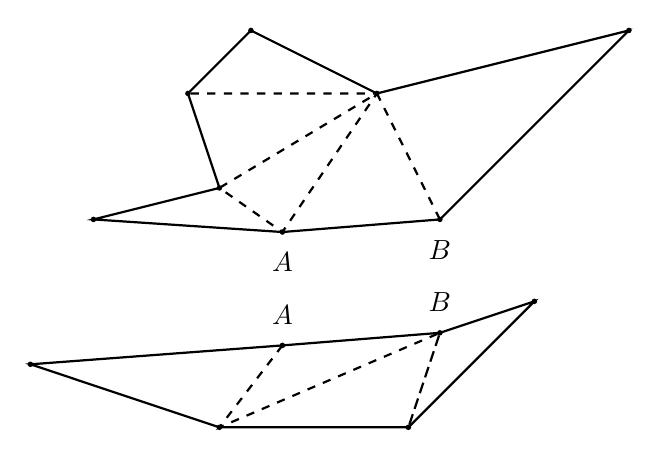
\begin{tikzpicture}[scale=.8]
\path
  (0,0) coordinate (A1) -- 
  ++(3,0) coordinate (B1) --
  ++(2,2) coordinate (C1) --
  ++(-1.5,-.5) coordinate (D1);
\draw[thick]
  (D1) --
  ++(3,3) coordinate (E1) -- 
  ++(-4,-1) coordinate (F1) --
  ++(-2,1) coordinate (G1) --
  ++(-1,-1) coordinate (H1) --
  ++(.5,-1.5) coordinate (I1) --
  ++(-2,-.5) coordinate (J1) --
  ++(3,-.2) coordinate (K1);
\path
  (K1) -- 
  ++(-4,-.3) coordinate (L1) --
  (A1);
  
\foreach \point in {D1,E1,F1,G1,H1,I1,J1,K1}
  \fill (\point) circle(1.25pt);

\node[below,yshift=-4pt] at (K1) {$A$};
\node[below,yshift=-4pt] at (D1) {$B$};

\draw[thick,dashed]
  (D1) -- (F1) -- (I1) -- (K1) -- (F1) -- (H1);
\draw[thick] (D1) -- (K1);

\begin{scope}[yshift=-1.8cm]

\draw[thick]
  (0,0) coordinate (A2) -- 
  ++(3,0) coordinate (B2) --
  ++(2,2) coordinate (C2) --
  ++(-1.5,-.5) coordinate (D2);
\path
  (D2) --
  ++(3,3) coordinate (E2) --
  ++(-4,-1) coordinate (F2) --
  ++(-2,1) coordinate (G2) --
  ++(-1,-1) coordinate (H2) --
  ++(.5,-1.5) coordinate (I2) --
  ++(-2,-.5) coordinate (J2) --
  ++(3,-.2) coordinate (K2);
\draw[thick]
  (K2) --
  ++(-4,-.3) coordinate (L2) --
  (A2);
  
\foreach \point in {A2,B2,C2,D2,K2,L2}
  \fill (\point) circle(1.25pt);
  
\node[above,yshift=4pt] at (K2) {$A$};
\node[above,yshift=4pt] at (D2) {$B$};

\draw[thick,dashed]
  (K2) -- (A2) -- (D2) -- (B2) -- (D2);
\draw[thick] (D2) -- (K2);

\end{scope}
\end{tikzpicture}
\end{center}
לפי הנחת האינדוקציה, ניתן לצבוע כל אחד מהמצולעים הללו בשלושה צבעים:
\begin{center}

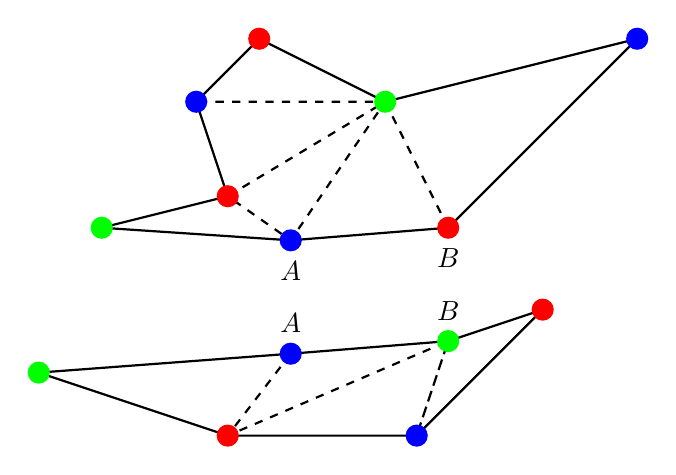
\begin{tikzpicture}[scale=.8]
\path
  (0,0) coordinate (A1) -- 
  ++(3,0) coordinate (B1) --
  ++(2,2) coordinate (C1) --
  ++(-1.5,-.5) coordinate (D1);
\draw[thick]
  (D1) --
  ++(3,3) coordinate (E1) -- 
  ++(-4,-1) coordinate (F1) --
  ++(-2,1) coordinate (G1) --
  ++(-1,-1) coordinate (H1) --
  ++(.5,-1.5) coordinate (I1) --
  ++(-2,-.5) coordinate (J1) --
  ++(3,-.2) coordinate (K1);
\path
  (K1) -- 
  ++(-4,-.3) coordinate (L1) --
  (A1);
  
\draw[thick,dashed]
  (D1) -- (F1) -- (I1) -- (K1) -- (F1) -- (H1);
\draw[thick] (D1) -- (K1);

\node[below,yshift=-4pt] at (K1) {$A$};
\node[below,yshift=-4pt] at (D1) {$B$};

\foreach \point/\color in {D1/red,E1/blue,F1/green,G1/red,H1/blue,I1/red,J1/green,K1/blue}
  \fill[color=\color] (\point) circle(5pt);


\begin{scope}[yshift=-1.8cm]

\draw[thick]
  (0,0) coordinate (A2) -- 
  ++(3,0) coordinate (B2) --
  ++(2,2) coordinate (C2) --
  ++(-1.5,-.5) coordinate (D2);
\path
  (D2) --
  ++(3,3) coordinate (E2) --
  ++(-4,-1) coordinate (F2) --
  ++(-2,1) coordinate (G2) --
  ++(-1,-1) coordinate (H2) --
  ++(.5,-1.5) coordinate (I2) --
  ++(-2,-.5) coordinate (J2) --
  ++(3,-.2) coordinate (K2);
\draw[thick]
  (K2) --
  ++(-4,-.3) coordinate (L2) --
  (A2);
  
\draw[thick,dashed]
  (K2) -- (A2) -- (D2) -- (B2) -- (D2);
\draw[thick] (D2) -- (K2);
\node[above,yshift=4pt] at (K2) {$A$};
\node[above,yshift=4pt] at (D2) {$B$};

\foreach \point/\color in {A2/red,B2/blue,C2/red,D2/green,K2/blue,L2/green}
  \fill[color=\color] (\point) circle(5pt);


\end{scope}
\end{tikzpicture}
\end{center}
השיוך של צבעים לקודקודים הוא שרירותי, כך שאם הקודקודים 
$A,B$
מקבלים צבעים שונים בשני המצולעים, ניתן לשנות את הצבעים באחד מהם כך שהצבעים של 
$A,B$
זהים בשני המצולעים. נחליף את הצבעים
\textbf{אדום}
ו-%
\textbf{ירוק}
במצולע התחתון:
\begin{center}

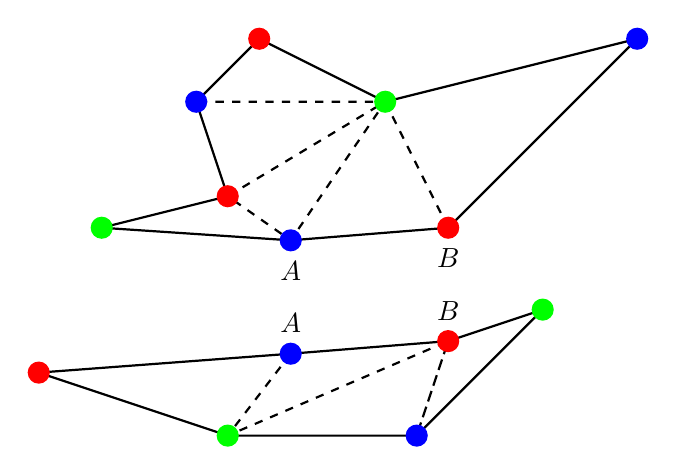
\begin{tikzpicture}[scale=.8]
\path
  (0,0) coordinate (A1) -- 
  ++(3,0) coordinate (B1) --
  ++(2,2) coordinate (C1) --
  ++(-1.5,-.5) coordinate (D1);
\draw[thick]
  (D1) --
  ++(3,3) coordinate (E1) -- 
  ++(-4,-1) coordinate (F1) --
  ++(-2,1) coordinate (G1) --
  ++(-1,-1) coordinate (H1) --
  ++(.5,-1.5) coordinate (I1) --
  ++(-2,-.5) coordinate (J1) --
  ++(3,-.2) coordinate (K1);
\path
  (K1) -- 
  ++(-4,-.3) coordinate (L1) --
  (A1);
  
\node[below,yshift=-4pt] at (K1) {$A$};
\node[below,yshift=-4pt] at (D1) {$B$};

\draw[thick,dashed]
  (D1) -- (F1) -- (I1) -- (K1) -- (F1) -- (H1);
\draw[thick] (D1) -- (K1);
\foreach \point/\color in {D1/red,E1/blue,F1/green,G1/red,H1/blue,I1/red,J1/green,K1/blue}
  \fill[color=\color] (\point) circle(5pt);

\begin{scope}[yshift=-1.8cm]

\draw[thick]
  (0,0) coordinate (A2) -- 
  ++(3,0) coordinate (B2) --
  ++(2,2) coordinate (C2) --
  ++(-1.5,-.5) coordinate (D2);
\path
  (D2) --
  ++(3,3) coordinate (E2) --
  ++(-4,-1) coordinate (F2) --
  ++(-2,1) coordinate (G2) --
  ++(-1,-1) coordinate (H2) --
  ++(.5,-1.5) coordinate (I2) --
  ++(-2,-.5) coordinate (J2) --
  ++(3,-.2) coordinate (K2);
\draw[thick]
  (K2) --
  ++(-4,-.3) coordinate (L2) --
  (A2);
  

\draw[thick,dashed]
  (K2) -- (A2) -- (D2) -- (B2) -- (D2);
\draw[thick] (D2) -- (K2);
\node[above,yshift=4pt] at (K2) {$A$};
\node[above,yshift=4pt] at (D2) {$B$};


\foreach \point/\color in {A2/green,B2/blue,C2/green,D2/red,K2/blue,L2/red}
  \fill[color=\color] (\point) circle(5pt);

\end{scope}
\end{tikzpicture}
\end{center}
כעת ניתן להדביק את שני המצולעים ביחד כדי לשחזר את המצולע המקורי עם
$n$
קודקודים. המצולע יהיה צבוע בשלושה צבעים.
\qed

\begin{center}
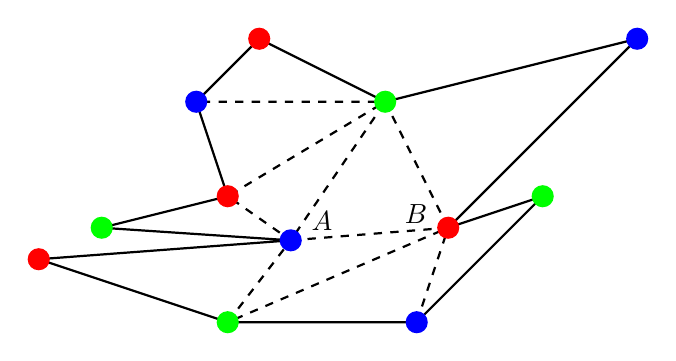
\begin{tikzpicture}[scale=.8]
\draw[thick]
  (0,0) coordinate (A) -- 
  ++(3,0) coordinate (B) --
  ++(2,2) coordinate (C) --
  ++(-1.5,-.5) coordinate (D) --
  ++(3,3) coordinate (E) -- 
  ++(-4,-1) coordinate (F) --
  ++(-2,1) coordinate (G) --
  ++(-1,-1) coordinate (H) --
  ++(.5,-1.5) coordinate (I) --
  ++(-2,-.5) coordinate (J) --
  ++(3,-.2) coordinate (K) -- 
  ++(-4,-.3) coordinate (L) --
  cycle;
  

\node[above right,xshift=4pt] at (K) {$A$};
\node[above left,xshift=-4pt,yshift=-2pt] at (D) {$B$};

\draw[thick,dashed]
  (B) -- (D) -- (K) -- (F) -- (I) -- (K) -- (A) -- (D) -- (F) -- (H);

\foreach \point/\color in {D/red,E/blue,F/green,G/red,H/blue,I/red,J/green,K/blue,A/green,B/blue,C/green,L/red}
  \fill[color=\color] (\point) circle(5pt);
\end{tikzpicture}
\end{center}


\section{מצביעת מצולעים לשמירה על מוזיאונים}

\begin{theorem}
$n/3$
שומרים יכולים לשמור מוזיאון עם 
$n$
קירות.
\end{theorem}

\textbf{הוכחה של משפט
\ref{thm.guarded}:}
לפי משפט
\ref{thm.tri}
ניתן לתלת את המצולע ולפי משפט
\ref{thm.colored}
ניתן לצבוע את המצולע בשלושה צבעים. שלושת הקודקודים של כל משולש יהיו צבועים בצבעים שונים, כך שכל צבע מופיע באחד הקודקודים של כל משולש. אם צובעים 
$n$
קודקודים בשלושה צבעים, צבע אחד לפחות )נניח אדום( מופיע לכל היותר
$\disfrac{n}{3}$
פעמים, ובכל משולש חייב להיות קודקוד צבוע אדום.

אם נציב שומרת בקודקוד אדום, היא יכולה לראות את הקירות של אותו משולש. כל המשולשים של תילות המצולע כוללים את כל הצלעות של המצולע, ולכן
$\disfrac{n}{3}$
שומרות מספיקות כדי לראות את כל הקירות של המוזיאון.
\qed

כעת נוכיח את משפט
\ref{thm.tri}
שניתן לתלת כל מצולע.

\section{ניתן לתלת כל מצולע}

\begin{theorem}\label{thm.interior-angles-of-a-polygon}\mbox{}\\
סכום הזוויות הפנימיות של מצולע עם
$n$
צלעות הוא
$180^\circ(n-2)$.
\end{theorem}



\textbf{הוכחה:}
תחילה נוכיח עבור מצולעים קמורים. נסמן את 
\textbf{הזוויות החיצוניות}
ב-%
$\theta_i$:
\begin{center}

\begin{tikzpicture}[scale=.6]
\coordinate (O) at (0,0);
%\fill (O) circle (2pt);
\foreach \x/\name/\n/\po in {0/a/A/right,.6/b/B/above,1.6/c/C/left,2.4/d/D/below left,3.9/e/E/below right} {
  \coordinate (\name) at ($(O)+(\x*72+18:3cm)$);
%  \fill (\name) circle (1.5pt);
%  \node[\po] at (\name) {$\n$};
%\draw[dashed] (O) -- (\name);
}
\draw[thick] (a) -- (b) -- (c) -- (d) --(e) -- cycle;

\draw[thick,dashed] (a) 
  node[above,xshift=-2pt,yshift=8pt] {$\theta_1$} -- 
  ($(a)!2!(b)$);
\draw[thick,dashed] (b)
  node[above left,xshift=-8pt,yshift=0pt] {$\theta_2$} -- 
  ($(b)!1.7!(c)$);
\draw[thick,dashed] (c) 
  node[below left,xshift=-4pt,yshift=-2pt] {$\theta_3$} -- 
  ($(c)!1.7!(d)$);
\draw[thick,dashed] (d)
  node[below right,xshift=0pt,yshift=-4pt] {$\theta_4$} -- 
  ($(d)!1.5!(e)$);
\draw[thick,dashed] (e)
  node[right,xshift=4pt,yshift=4pt] {$\theta_5$} -- 
  ($(e)!1.7!(a)$);

\end{tikzpicture}
\end{center}
אם נסכם את הזוויות החיצוניות נקבל 
$\displaystyle\sum_{i=1}^n \theta_i = 360^\circ$.
ניתן לראות את הסיכום באיור על ידי "סיבוב" הקווים המקווקווים מאחד לשני לפי הסדר 
$\theta_1,\ldots,\theta_5$.
עבור כל זוית חיצונית
$\theta_i$
נסמן את הזוית הפנימית של אותו קודקוד ב-%
$\phi_i$.
נחשב:
\begin{eqn}
\displaystyle\sum_1^n \theta_i &=&\displaystyle\sum_1^n (180^\circ-\phi_i)= 360^\circ\\
%n\cdot 180^\circ-\displaystyle\sum_1^n \phi_i &=& 360^\circ\\
\displaystyle\sum_1^n \phi_i &=& n\cdot 180^\circ-360^\circ =180^\circ(n-2)\,.
\end{eqn}
נבדוק מה קורה אם נוסיף קודקוד קעור:
\begin{center}

\begin{tikzpicture}
\draw[thick] (0,0) -- (3,0) coordinate (A) node[above left,yshift=8pt] {$\alpha$} -- ++(60:2) coordinate (B) node[above,yshift=8pt] {$\beta$} -- ++(-60:2) coordinate (C) node[above right,yshift=8pt] {$\gamma$}  -- ++(3,0);

\draw ($(A)+(-.4,0)$) arc(180:60:.4);
\draw ($(B)+(-60:.3)$) arc(-60:240:.3);
\draw ($(C)+(.4,0)$) arc(0:120:.4);

\draw[thick,dashed] (A) -- (C);
\end{tikzpicture}
\end{center}
קיים משולש המורכב משתי הצלעות שנוגעות בקודקוד הקעור והצלע המסומן בקו מקווקוו. נסכם את הזוויות של המשולש:

\begin{eqn}
(180^\circ - \alpha) + (360^\circ - \beta) + (180^\circ - \gamma) &=& 180^\circ\\
\alpha + \beta + \gamma &=& 3\cdot 180^\circ\,.
\end{eqn}
סכום הזוויות הפנימיות גדל ב-%
$\alpha+\beta+\gamma$
ומספר הקודקודים גדל בשלוש:

\begin{eqn}
\displaystyle\sum_1^n \phi_i + (\alpha + \beta + \gamma) &=& 180^\circ(n-2)+3\cdot 180^\circ\\
&=& 180^\circ((n+3)-2)\,.
\end{eqn}
\qed



\begin{theorem}\label{thm.convex}\mbox{}\\
חייב להיות לפחות שלושה קודקודים קמורים במצולע.
\end{theorem}



\textbf{הוכחה:}
נסמן ב-%
$k$
את מספר הקודקודים הקעורים, כאשר הזווית הפנימית של כל אחד הוא
$180^\circ+\epsilon_i$, $\epsilon_i>0$.
סכום הזוויות הפנימיות של הקודקודים
\textbf{הקעורים}
הוא בוודאי פחות או שווה לסכום
\textbf{כל}
הזוויות הפנימיות:

\begin{eqn}
k\cdot 180^\circ +\displaystyle\sum_{i=1}^{k}\epsilon_i &\leq& 180^\circ(n-2)\\
k\cdot 180^\circ  &<& 180^\circ(n-2)\\
%(k+2)\cdot 180^\circ &<& n\cdot 180^\circ\\
k&<&n-2\,.
\end{eqn}
מכאן שיש לא רק קודקוד אחד, אבל לפחות שלושה קודקודים שאינם קעורים.
\qed

\textbf{הוכחה של משפט
\ref{thm.tri}:}
באינדוקציה על מספר הקודקודים. עבור
$n=3$
אין מה להוכיח. נניח ש-%
$n>3$.
לפי משפט 
\ref{thm.convex},
חייב להיות קודקוד קמור
$C$.
סמנו את הקודקודים השכנים שלו
$B,D$.
אם
$\overline{BD}$
נמצא כולו בתוך המצולע אז הוא אלכסון וניתן לחלק את המצולע למשולש 
$\triangle BCD$
ולמצולע קטן יותר כאשר
$\overline{BD}$
הוא צלע.

\begin{center}

\begin{tikzpicture}[scale=1.6]
\clip (-2,-.2) rectangle (3.8,2.2);
\draw[thick]
  (0,0) coordinate (A) -- 
  ++(1.5,0) coordinate (B) --
  ++(2,2) coordinate (C) --
  ++(-1.8,-.5) coordinate (D) --
  ++(-1,.5) coordinate (E) --
%  ++(1.3,-1) coordinate (F) --
  (A);
\draw[thick,dashed] (B) -- (D);
%\draw[very thick,dotted] (C) -- (F);
%\node [draw,circle through=(F)] at (C) {};
\foreach \point/\pos in {A/below,B/below,C/right,D/above,E/left}
  \fill (\point) circle(.7pt) node[\pos] {$\point$};
\end{tikzpicture}
\end{center}


לפי הנחת האינדוקציה, ניתן לתלת את המצולע ואז להדביק אותו למשולש
$\triangle BCD$
ולקבל תילות של המצולע המקורי. אחרת, חייב להיות קודקוד קעור
$F$
הקרוב ביותר ל-%
$C$,
ולכן
$\overline{CF}$
הוא אלכסון המחלק את המצולע לשני מצולעים קטנים יותר. לפי הנחת האינדוקציה ניתן לתלת אותם ולהדביק אותם אחד לשני.
\begin{center}

\begin{tikzpicture}[scale=1.6]
\clip (-2,-.2) rectangle (3.8,2.2);
\draw[thick]
  (0,0) coordinate (A) -- 
  ++(1.5,0) coordinate (B) --
  ++(2,2) coordinate (C) --
  ++(-1.8,-.5) coordinate (D) --
  ++(-1,.5) coordinate (E) --
  ++(1.3,-1) coordinate (F) --
  (A);
%\draw[thick,dashed] (B) -- (D);
\draw[very thick,dashed] (C) -- (F);
\node [draw,circle through=(F)] at (C) {};
\foreach \point/\pos in {A/below,B/below,C/right,D/above,E/left,F/below}
  \fill (\point) circle(.7pt) node[\pos] {$\point$};
\end{tikzpicture}
\end{center}

\selectlanguage{hebrew}


\subsection*{מקורות}

פרק זה מבוסס על פרק~$39$ ב-%
\cite{thebook}.


\tikzsetfigurename{langford}
% !TeX root = surprises.tex

\selectlanguage{hebrew}


\chapter{הבעיה של 
\L{Langford}}
\label{c.langford}

המתמטיקאי
\L{C. Dudley Langford}
שם לב שבנו סידר קוביות צבעוניות לפי הסדר:
\begin{figure}
\begin{center}

\begin{tikzpicture}
\draw[rounded corners,fill=green] (0,0)  
  rectangle +(1.6cm,.8cm);
\draw[rounded corners,fill=red]   (2.2,0)
  rectangle +(1.6cm,.8cm);
\draw[rounded corners,fill=blue]  (4.4,0)
  rectangle +(1.6cm,.8cm);
\draw[rounded corners,fill=red]   (6.6,0)
  rectangle +(1.6cm,.8cm);
\draw[rounded corners,fill=green] (8.8,0)
  rectangle +(1.6cm,.8cm);
\draw[rounded corners,fill=blue]  (11,0)
  rectangle +(1.6cm,.8cm);
\end{tikzpicture}
\end{center}
\caption{}\label{}
\end{figure}

קוביה אחת נמצאת בין שתי הקוביות האדומות, שתי קוביות בין הקוביות הכחולות, ושלוש קוביות בין הקוביות הירוקות. ניתן לנסח את הבעיה כך:
נתון שק%
\footnote{\R{
שק הוא  קבוצה בה איבר יכול להופיע מספר פעמים}.} של מספרים
$\{1,1,2,2,3,3\}$,
האם אפשר לסדר אותם בסדרה כך שלכל
$1\leq i \leq 3$,
$i$
מספרים נמצאים בין שני המופעים של
$i$?

\textbf{
הבעיה של
\L{Langford} $L(n)$}:
נתון שק של מספרים
$\{1,1,2,2,3,3,\ldots,n,n\}$,
האם ניתן לסדר אותם כך שלכל
$1\leq i \leq n$, $i$
מספרים נמצאים בין שני המופעים של
$i$?


מהאיור לעיל אנו רואים שעבור 
$n=3$
הפתרון הוא
$312132$.


%%%%%%%%%%%%%%%%%%%%%%%%%%%%%%%%%%%%%%%%%%%%%%
\selectlanguage{hebrew}


\section{
הבעיה של
\L{Langford}
כבעיית כיסוי}

ניתן להציג את הבעיה של
\L{Langford}
באמצעות טבלה. עבור
$L(3)$
יש
$6$
עמודות, אחת לכל מקום בסדרה. השורות מציגות את כל האפשרויות לסדר את  שני המופעים של המספרים. קל לראות שיש ארבעה זוגות של מקומות אפשריים עבור
$1$,
שלושה עבור
$2$
ושניים עבור
$3$:
%)טבלה~%
%\ref{t.lang3:1}(.

%\begin{table}
\[
\begin{array}{|c||c|c|c|c|c|c|}
\hline
&1&2&3&4&5&6\\\hline\hline
1&1&&1&&&\\\hline
2&&1&&1&&\\\hline
3&&&1&&1&\\\hline
4&&&&1&&1\\\hline
5&2&&&2&&\\\hline
6&&2&&&2&\\\hline
7&&&2&&&2\\\hline
8&3&&&&3&\\\hline
9&&3&&&&3\\\hline
\end{array}
\]
%\caption{סידורים אפשריים}\label{t.lang3:1}
%\end{table}


כדי לפתור את הבעיה, עלינו לבחור שורה אחת עבור המופעים של
$1$,
שורה אחת עבור המופעים של
$2$
ושורה אחת עבור המופעים של
$3$,
כך שאם הנמקם את השורות אחת מעל לשניה, בכל עמודה יש רק מספר אחד: 
%)טבלה~%
%\ref{t.lang3:2}(.

%\begin{table}
\[
\begin{array}{|c||c|c|c|c|c|c|}
\hline
&1&2&3&4&5&6\\\hline\hline
2&&1&&1&&\\\hline
7&&&2&&&2\\\hline
8&3&&&&3&\\\hline
\end{array}
\]
%\caption{סידור סופי}\label{t.lang3:2}
%\end{table}


שורה
$9$
אינה נחוצה בגלל סימטריה: סדרה המתחילה עם השורה
$9$
זהה לסדרה מתקבלת מהפיכת הסדר של סדרה המתקבלת כאשר מתחילים עם שורה
$8$.

שורה 
$8$
היא היחידה המכילה את המספר
$3$
כך שחובה לבחור אותה, והסדרה המתקבלת היא
$3\sqcup  \sqcup  \sqcup  3\sqcup $. 
אי אפשר להשתמש בכל שורה שיש לה מספרים בעמודות
$1$
ו-
$5$,
כי מותר רק מספר אחד בכל מקום. נסמן את השורות שניתן לבחור ושלא ניתן לבחור כך:
$\not 1,2,\not 3,4,\not 5, \not 6, 7, 8$.

שורה
$7$
היא השורה האפשרית היחידה עבור
$2$
כך שחובה לבחור בה והתוצאה היא
$3\sqcup  2\sqcup  3{}2$.
נעדכן את רשימת השורות ונקבל:
$\not 1,2,\not 3,\not 4,\not 5, \not 6, 7, 8$.

כעת, ניתן לבחור רק שורה
$2$
ומתקבל הפתרון
$3{}1{}2{}1{}3{}2$.

טבלה~%
~\ref{t.lang4}
היא הטבלה עבור
$L(4)$.
הפתרון הוא
$41312432$.

\selectlanguage{hebrew}
\begin{table}
\[
\begin{array}{|c||c|c|c|c|c|c|c|c|}
\hline
&1&2&3&4&5&6&7&8\\\hline\hline
1&1&&1&&&&&\\\hline
2&&1&&1&&&&\\\hline
3&&&1&&1&&&\\\hline
4&&&&1&&1&&\\\hline
5&&&&&1&&1&\\\hline
6&&&&&&1&&1\\\hline
7&2&&&2&&&&\\\hline
8&&2&&&2&&&\\\hline
9&&&2&&&2&&\\\hline
10&&&&2&&&2&\\\hline
11&&&&&2&&&2\\\hline
12&3&&&&3&&&\\\hline
13&&3&&&&3&&\\\hline
14&&&3&&&&3&\\\hline
15&&&&3&&&&3\\\hline
16&4&&&&&4&&\\\hline
17&&4&&&&&4&\\\hline
18&&&4&&&&&4\\\hline
\end{array}
\]
\selectlanguage{hebrew}
\caption{הבעיה של Langford $L(4)$}\label{t.lang4}
\end{table}

\selectlanguage{hebrew}


\section{
עבור איזה ערכים של
$n$
ניתן לפתור את הבעיה}
\begin{theorem}\mbox{}\\
ניתן למצוא פתרון ל-%
$L(n)$
אם ורק אם
$n=4k$
או
$n=4k-1$.
\end{theorem}
נוכיח רק שאם 
$n=4k-2$
או
$n=4k-3$
אין פתרון לבעיה.

\textbf{הוכחה 1}

אם המופע הראשון של המספר
$k$
נמצא במקום
$i_k$,
המופע השני נמצא במקום
$i_k+k+1$.
לכן,
$S_n$,
סכום המקומות של כל המספרים, הוא:

\begin{eqn}
S_n&=&\sum_{k=1}^{n}i_k+\sum_{k=1}^{n}(i_k+k+1)\\
& =& 2\sum_{k=1}^{n}i_k+\sum_{k=1}^{n}(k+1)\\
&=& 2\sum_{k=1}^{n}i_k+\frac{n(n+3)}{2}\,.
\end{eqn}
אבל
$S_n$
הוא פשוט
$1+2+3+\cdots+2n$
ולפי הנוסחה לסיכום סדרת מספרים:
\[
S_n=\sum_{k=1}^{2n}k = \frac{2n(2n+1)}{2}\,.
\]
נשווה את שני הביטויים עבור
$S_n$:

\begin{eqn}
2\sum_{k=1}^{n}i_k+\frac{n(n+3)}{2} &=& \frac{2n(2n+1)}{2}\\
\sum_{k=1}^{n}i_k &=& \frac{1}{2}\left(\frac{2n(2n+1)}{2} - \frac{n(n+3)}{2}\right) \\
&=& \frac{3n^2-n}{4}\,.
\end{eqn}

הצד השמאלי חייב להיות מספר שלם כי הוא סכום של מספרים שלמים. לכן, הצד הימני חייב גם הוא להיות מספר שלם, כלומר,
$3n^2-n=n(3n-1)$
חייב להתחלק ב-%
$4$.
\begin{itemize}
\item
אפשרות אחת היא ש-%
$n$
בעצמו מתחלק ב-%
$4$.
\item

מתי 
$3n-1$
מתחלק ב-%
$4$?
ניתן להציג את
$n$
כ-%
$n=4i+j$
עבור
$j=0,1,2,3$.
אם 
$3n-1$
מתחלק ב-%
$4$,
גם
$3(4i+j)-1 = 12i+3j-1$
מתחלק ב-%
$4$.
$12i$
מתחלק ב-%
$4$,
וקל לראות ש-%
$3j-1$
מתחלק ב-%
$4$
)עבור 
$j=0,1,2,3$%
( רק אם
$j=3$.
מכאן ש-%
$3n-1$
מתחלק ב-%
$4$
רק עבור
$n=4i+3=4(i+1)-1=4k-1$.
\end{itemize}
\qed



\textbf{הוכחה
\L{2}}


נעיין בפתרון עבור
$n=4$
ונבדוק תחילה את מקומות המופעים של המספרים הזוגיים:
\[
\begin{array}{|c|c|c|c|c|c|c|c|}
\hline
1&2&3&4&5&6&7&8\\
\hline\hline
4&1&3&1&2&4&3&2\\\hline
*&&&&&*&&\\\hline
\end{array}
\hspace{3em}
\begin{array}{|c|c|c|c|c|c|c|c|}
\hline
1&2&3&4&5&6&7&8\\
\hline\hline
4&1&3&1&2&4&3&2\\\hline
&&&&*&&&*\\\hline
\end{array}
\]
מקומות המופעים של
$4$
הם
$1$
ו-%
$6$,
ומקומות המופעים של
$2$
הם
$5$
ו-%
$8$.
ניקח מספר
\textbf{זוגי}
$k=2m$. 
מקום המופע הראשון שלו הוא
$i$
ומקום המופע השני שלו הוא
$i+k+1$.
סכום המקומות הוא:
\[
i+(i+k+1)=2i+2m+1=2(i+m)+1
\]
שהוא מספר אי-זוגי.
סכום של שני מספרים הוא אי-זוגיים אם ורק אם אחד זוגי והשני אי-זוגי.

נבדוק עכשיו את מקומות המופעים של המספרים האי-זוגיים:

\[
\begin{array}{|c|c|c|c|c|c|c|c|}
\hline
1&2&3&4&5&6&7&8\\
\hline\hline
4&1&3&1&2&4&3&2\\\hline
&*&&*&&&&\\\hline
\end{array}
\hspace{3em}
\begin{array}{|c|c|c|c|c|c|c|c|}
\hline
1&2&3&4&5&6&7&8\\
\hline\hline
4&1&3&1&2&4&3&2\\\hline
&&*&&&&*&\\\hline
\end{array}
\]
מקומות המופעים של
$1$
הם
$2$
ו-%
$4$,
ומקומות המופעים של
$3$
הם
$3$
ו-%
$7$.
ניקח מספר 
\textbf{אי-זוגי},
$k=2m+1$.
מקום המופע הראשון שלו הוא
$i$
ומקום המופע השני שלו הוא
$i+k+1$.
סכום המקומות הוא:
\[
i+(i+k+1)=2i+2m+1+1=2(i+m+1)\,,
\]
שהוא מספר זוגי.
סכום של שני מספרים הוא זוגי אם ורק אם שניהם זוגיים או שניהם אי-זוגיים.

ברור שרשימת המקומות של המספרים בסדרה,
$1,2,\ldots,2n-1,2n$,
מכילה מספר שווה של מקומות זוגיים ומקומות אי-זוגיים. כאשר מציבים את שני המופעים של מספר בסדרה, הם "תופסים" שני מקומות. כאשר מסיימים להציב את כל המספרים בפתרון, חייבים להיות מספר שווה של מקומות זוגיים ואי-זוגיים "שנתפסו".

\textbf{זוגיות}
היא ההפרש בין מספר המקומות הזוגיים שנתפסו לבין מספר המקומות האי-זוגיים שנתפסו. תחילה הזוגיות היא אפס, ואם יש פתרון זוגיות שלו גם כן אפס. אנו נמצא את התנאים על 
$n$ 
כך שהזוגיות לא תתאפס. עבור ערכים אלה אין פתרון.

כאשר ממקמים את שני המופעים של מספר זוגי, הם תופסים מקום אחד זוגי )מסומן 
$+1$(
ומקום אחר אי-זוגי )מסומן 
$-1$(,
וסכום הזוגיות הוא אפס.
\[
\begin{array}{|c|c|c|c|c|c|c|c|}
\hline
1&2&3&4&5&6&7&8\\
\hline\hline
4&1&3&1&2&4&3&2\\\hline
-1&&&&&+1&&\\\hline
\end{array}
\hspace{3em}
\begin{array}{|c|c|c|c|c|c|c|c|}
\hline
1&2&3&4&5&6&7&8\\
\hline\hline
4&1&3&1&2&4&3&2\\\hline
&&&&-1&&&+1\\\hline
\end{array}
\]

כאשר ממקמים את שני המופעים של מספר אי-זוגי,  הם תופסים שני מקומות זוגיים )מסומן 
$+1$(
או שני מקומות אי-זוגיים )מסומן 
$-1$(,
וסכום הזוגיות היא
$\pm 2$.
\[
\begin{array}{|c|c|c|c|c|c|c|c|}
\hline
1&2&3&4&5&6&7&8\\
\hline\hline
4&1&3&1&2&4&3&2\\\hline
&+1&&+1&&&&\\\hline
\end{array}
\hspace{3em}
\begin{array}{|c|c|c|c|c|c|c|c|}
\hline
1&2&3&4&5&6&7&8\\
\hline\hline
4&1&3&1&2&4&3&2\\\hline
&&-1&&&&-1&\\\hline
\end{array}
\]
כדי שהזוגיות תתאפס
\textbf{חייב להיות מספר זוגי של מספרים אי-זוגיים ב}-%
$\{1,\ldots,n\}$!
נוכיח שאם 
$n=4k, 4k\!-\!1$
יש מספר זוגי של אי-זוגיים )וכנראה שיש פתרון(,
ואם
$n=4k\!-\!2, 4k\!-\!3$
יש מספר אי-זוגי של אי-זוגיים )ואין פתרון(.

ההוכחה באינדוקציה. עבור 
$k=1$:
\begin{itemize}
\item $n=4k-3=1$.
ב-%
$\{1\}$
יש מספר אי-זוגי של אי-זוגיים )וברור שאין פתרון(.
\item $n=4k-2=2$.
ב-%
$\{1,2\}$
יש מספר אי-זוגי של אי-זוגיים )וברור שאין פתרון(.
\item $n=4k-1=3$.
ב-%
$\{1,2,3\}$
יש מספר זוגי של אי-זוגיים )וראינו שיש פתרון(.
\item $n=4k-0=4$.
ב-%
$\{1,2,3,4\}$
יש מספר זוגי של אי-זוגיים )וראינו שיש פתרון(.
\end{itemize}

נניח שהטענה נכונה עבור 
$n=4k-j, k\geq 1, 0\leq j\leq 3$,
ונוכיח שהטענה נכונה עבור
$n=4(k+1)-j, k\geq 1, 0\leq j\leq 3$.
\begin{itemize}
\item
נוסיף לשק את המספר הבא אחרי 
$4k$
שהוא
$4k+1=4(k+1)-3$.
לפי הנחת האינדוקציה עבור  
$n=4k-0$
יש מספר זוגי של אי-זוגיים. 
$4(k+1)-3$
הוא אי-זוגי ולכן יש עכשיו מספר אי-זוגי של אי-זוגיים )אין פתרון(.

\item
נוסיף לשק את המספר הבא אחרי 
$4k+1$
שהוא
$4k+2=4(k+1)-2$.
הוכחנו שעבור
$n=4k+1$
יש מספר אי-זוגי של אי-זוגיים. 
$4(k+1)-2$
הוא זוגי ולכן עדיין יש מספר אי-זוגי של אי-זוגיים )אין פתרון(.

\item
נוסיף לשק את המספר הבא אחרי 
$4k+2$
שהוא
$4k+3=4(k+1)-1$.
הוכחנו שעבור
$n=4k+2$
יש מספר אי-זוגי של אי-זוגיים. 
$4(k+1)-1$
הוא אי-זוגי ולכן עכשיו יש מספר זוגי של אי-זוגיים )כנראה שיש פתרון(.

\item
נוסיף לשק את המספר הבא אחרי 
$4k+3$
שהוא
$4k+4=4(k+1)-0$.
הוכחנו שעבור
$n=4k+3$
יש מספר זוגי של אי-זוגיים. 
$4(k+1)-0$
הוא זוגי ולכן עדיין יש מספר זוגי של אי-זוגיים )כנראה שיש פתרון(.

\end{itemize}


%%%%%%%%%%%% Solution for L(4) %%%%%%%%%%%%%%%%%%

\section{פתרון עבור
$L(4)$}\label{s.langford-four}

Here is the array for $L(4)$. Try to find the solution yourself.
\begin{center}
\addtolength{\tabcolsep}{4pt}
\begin{tabular}{|c||c|c|c|c|c|c|c|c|}
\hline
&1&2&3&4&5&6&7&8\\\hline\hline
1&1&&1&&&&&\\\hline
2&&1&&1&&&&\\\hline
3&&&1&&1&&&\\\hline
4&&&&1&&1&&\\\hline
5&&&&&1&&1&\\\hline
6&&&&&&1&&1\\\hline
7&2&&&2&&&&\\\hline
8&&2&&&2&&&\\\hline
9&&&2&&&2&&\\\hline
10&&&&2&&&2&\\\hline
11&&&&&2&&&2\\\hline
12&3&&&&3&&&\\\hline
13&&3&&&&3&&\\\hline
14&&&3&&&&3&\\\hline
15&&&&3&&&&3\\\hline
16&4&&&&&4&&\\\hline
17&&4&&&&&4&\\\hline
18&&&4&&&&&4\\\hline
\end{tabular}
\end{center}
By symmetry row 18 may be eliminated.

\smallskip

%$1,2,3,4,5,6,7,8,9,10,11,12,13,14,15,16,17$
\noindent Choose row 16 and the sequence is 4\textvisiblespace\textvisiblespace\textvisiblespace\textvisiblespace 4 \textvisiblespace\textvisiblespace.
Any row with an element in position $1$ or position $6$ can no longer be part of the solution.

$\not\! 1,2,3,\not\! 4,5,\not\! 6,\not\! 7,8,\not\! 9,10,11,\not\!\! 12,\not\!\! 13,14,15,16,\not\!\! 17$

\noindent Choose row 14 and the sequence is 4\textvisiblespace 3\textvisiblespace\textvisiblespace 4{}3\textvisiblespace.

$\not\! 1,2,\not\! 3,\not\! 4,\not\! 5,\not\! 6,\not\! 7,8,\not\! 9,\not\!\! 10,11,\not\!\! 12,\not\!\! 13,14, \not\!\! 15,16,\not\!\! 17$

\noindent Choose row 8. The sequence is 4{}2{}3\textvisiblespace 2{}4{}3\textvisiblespace.

$\not\! 1,\not\! 2,\not\! 3,\not\! 4,\not\! 5,\not\! 6,\not\! 7,8,\not\! 9,\not\!\! 10,\not\!\! 11,\not\!\! 12,\not\!\! 13,14, \not\!\! 15,16,\not\!\! 17$

\noindent All of the choices for 1's have been eliminated so we must backtrack.

\smallskip

\noindent Instead of row 8 choose row 11 and the sequence is 4\textvisiblespace 3\textvisiblespace 2{}4{}3{}2.


$\not\! 1,2,\not\! 3,\not\! 4,\not\! 5,\not\! 6,\not\! 7,\not\! 8,\not\! 9,\not\!\! 10,11,\not\!\! 12,\not\!\! 13,14, \not\!\! 15,16,\not\!\! 17$

\noindent Choose row 2 and we have a solution 4{}1{}3{}1{}2{}4{}3{}2.

\smallskip

\noindent Continue backtracking to see if there is another solution.

\smallskip

\noindent Instead of row 14 choose row 15 and the sequence is 4\textvisiblespace \textvisiblespace 3\textvisiblespace 4\textvisiblespace 3.

$\not\! 1,\not\! 2,3,\not\! 4,5,\not\! 6,\not\! 7,8,\not\! 9,\not\!\! 10,\not\!\! 11,\not\!\! 12,\not\!\! 13,\not\!\! 14,15,16,\not\!\! 17$

\newpage

\noindent Row 8 must be chosen and the sequence is 4{}2\textvisiblespace 3{}2{}4\textvisiblespace 3.

$\not\! 1,\not\! 2,\not\! 3,\not\! 4,\not\! 5,\not\! 6,\not\! 7,8,\not\! 9,\not\!\! 10,\not\!\! 11,\not\!\! 12,\not\!\! 13,\not\!\! 14,15,16,\not\!\! 17$

\noindent All of the choices for 1's have been eliminated so again we backtrack.

\smallskip

\noindent Instead of row 16 choose row 17 and the sequence is \textvisiblespace 4\textvisiblespace \textvisiblespace \textvisiblespace\textvisiblespace 4\textvisiblespace.

$1,\not\! 2,3,4,\not\! 5,6,7,\not\! 8,9,\not\!\! 10,11,12,\not\!\! 13,\not\!\! 14,15,\not\!\! 16,17$

\noindent Choose row 15 and the sequence is \textvisiblespace 4\textvisiblespace 3\textvisiblespace\textvisiblespace 4{}3.

$1,\not\! 2,3,\not\! 4,\not\! 5,\not\! 6,\not\! 7,\not\! 8,9,\not\!\! 10,\not\!\! 11,\not\!\! 12,\not\!\! 13,\not\!\! 14,15,\not\!\! 16,17$

\noindent Row 9 must be chosen and the sequence is \textvisiblespace 4{}2{}3\textvisiblespace 2{}4{}3.

$1,\not\! 2,\not\! 3,\not\! 4,\not\! 5,\not\! 6,\not\! 7,\not\! 8,9,\not\!\! 10,\not\!\! 11,\not\!\! 12,\not\!\! 13,\not\!\! 14,15,\not\!\! 16,17$

\noindent All of the choices for 1's have been eliminated. We can backtrack one last time. 
%$1,\not\! 2,3,4,\not\! 5,6,7,\not\! 8,9,\not\! 10,11,12,\not\! 13,\not\! 14,15,\not\! 16,17$

\smallskip

\noindent Instead of row 15 choose row 12 and the sequence is 3{}4\textvisiblespace \textvisiblespace 3\textvisiblespace 4.

$\not\! 1,\not\! 2,\not\! 3,\not\! 4,\not\! 5,\not\! 6,\not\! 7,\not\! 8,9,\not\!\! 10,\not\!\! 11,12,\not\!\! 13,\not\!\! 14,\not\!\! 15,\not\!\! 16,17$

\noindent Again, all of the choices for 1's have been eliminated.

\medskip

\noindent Therefore the only solution is $41312432$.

\subsection*{What Is the Surprise?}

The source of the inspiration for a mathematical theorem can be surprising. Langford noticed a pattern in his son's colored blocks which led to the interesting Thm.~\ref{thm.langford}. Students should also be introduced to the fact that a theorem  can have many completely different proofs.

\subsection*{מקורות}
פרק זה מבוסס על
\L{\cite{miller}}.
\L{Davies}
מראה איך למצוא פתרון כאשר הזוגיות היא אפס.


%%%%%%%%%%%%%%%%% Number theory

\tikzsetfigurename{quadratic}
% !TeX root = surprises.tex

\chapter{Solving Quadratic Equations}\label{c.quadratic}

%%%%%%%%%%%%%%%%%%%%%%%%%%%%%%%%%%%%%%%%%%%%%%%%%%%%%%%%%%%%%%%

\abstract*{This chapter presents Poh-Shen Loh method for solving quadratic equations that is based on a relation between the coefficients of the quadratic polynomial and its roots. Al-Khwarizmi's geometric solution of quadratic equations in presented along with Cardano's geometric construction used to development the formula for finding roots of cubic equations.}

%%%%%%%%%%%%%%%%%%%%%%%%%%%%%%%%%%%%%%%%%%%%%%%%%%%%%%%%%%%%%%%

Poh-Shen Loh\index{Loh, Poh-Shen} proposed a method for solving quadratic equations that is based on a relation between the coefficients of the quadratic polynomial and its roots. Section~\ref{s.traditional} reviews the traditional methods for solving quadratic equations. 
Section~\ref{s.computing} tries to convince the reader that Loh's method makes sense and then explains how to compute the roots. In Sect.~\ref{s.examples} the computation is carried out for two quadratic polynomials and a similar computation for a quartic polynomial. Section~\ref{s.general} derives the traditional formula for the roots from Loh's formulas.

The introduction of algebra and modern algebraic notation is relatively recent. Previously, mathematicians used geometry almost exclusively, so it is interesting to look at al-Khwarizmi's geometric construction of the formula for the roots of quadratic equations (Sect.~\ref{s.khwar}). Section~\ref{s.cardano} shows a clever geometric construction used by Cardano in developing the formula for the roots of cubic equations.

Section~\ref{s.lill-quadratic} presents other geometric methods for finding the roots of quadratic equations.\footnote{Chapter~\ref{c.origami-cube} is a prerequisite for a full understanding of these methods.} The chapter concludes with Sect.~\ref{s.numerical} which discusses numerical computation of the roots of quadratic equations.

\section{Traditional Methods for Solving Quadratic Equations}\label{s.traditional}
\index{Quadratic equation}
Every student of mathematics memorizes the formula for obtaining the roots of a quadratic equation $ax^2+bx+c=0$:
\[
x_1, x_2 = \frac{-b\pm\sqrt{b^2-4ac}}{2a}\,.
\]                      

\newpage

For now we will work with monic\index{Monic polynomial} polynomials, $x^2+bx+c=0$, whose roots are:
\begin{align}
x_1, x_2 = \frac{-b\pm\sqrt{b^2-4c}}{2}\,.\label{eq.quadratic-roots}
\end{align}
Another method of solving quadratic equations is by factoring the polynomials more-or-less by trial-and-error. Sometimes it is easy to obtain the roots by factoring:
\begin{align}
x^2-4x+3= (x-1)(x-3)\label{eq.quadratic-lill}\,.
\end{align}
It is much harder to factor $x^2-2x-24$ because there are many possible pairs of roots that must be considered:
\[
(\pm 1,\mp 24)\,, (\pm 2,\mp 12)\,, (\pm 3,\mp 8)\,, (\pm 4,\mp 6)\,.
\]

\section{The Relation Between the Roots and the Coefficients}\label{s.computing}
\index{Quadratic equation!roots of}
\begin{theorem}\label{thm.roots-coefficients}
If $r_1,r_2$ are the roots of $x^2+bx+c$ then:
\[
(x-r_1)(x-r_2)=x^2 - (r_1+r_2)x + r_1r_2=x^2+bx+c\,.
\]
Therefore, even if we do not know the values of the roots, we do know that:
\begin{align}\label{eq.viete-quad}
r_1+r_2 = -b\,,\quad\quad r_1r_2=c\,.
\end{align}
\end{theorem}

There is really nothing to prove because the result emerges from the computation.

Consider some values of $-b,r_1,r_2$ and let $m_{12}$ be the average of $r_1,r_2$:
\[
\renewcommand{\arraystretch}{1.2}
\begin{array}{|@{\hspace{1em}}r|@{\hspace{1em}}r|@{\hspace{1em}}r|@{\hspace{1em}}r|}
\hline
-b& r_1 & r_2 &m_{12}\\\hline
33 & 12 & 21 & 16\frac{1}{2}\\\hline
33 & 8 & 25 & 16\frac{1}{2}\\\hline
33 & 1 & 32 & 16\frac{1}{2}\\\hline\hline
-b& r_1 & r_2 &m_{12}\\\hline
-4 & -16 & 12 & -2 \\\hline
-4 & -4 & 0 & -2 \\\hline
-4 & -3 & -1 & -2 \\\hline
\end{array}
\]

For any quadratic equation the average of the two roots is constant:
\[
m_{1,2}=\frac{r_1+r_2}{2}=
\frac{(-b-r_2)+r_2}{2}=
-\frac{b}{2}\,.
\]

\newpage

Let $s$ be any number. Then:
\[
-b=-b+s+(-s)=\left(\frac{-b}{2}+s\right) + \left(\frac{-b}{2}-s\right)=r_1+r_2\,.
\]
If one root is at distance $s$ from the average, the other root is at distance $-s$ from  the average. For $r_1,r_2=2,6$, where $m_{12}=4, s=2$, we have:
\[
\renewcommand{\arraystretch}{1.2}
\begin{array}{|@{\hspace{1em}}r|@{\hspace{1em}}r|@{\hspace{1em}}r|@{\hspace{1em}}r|r|r|}
\hline
-b& r_1 & r_2 & m_{12}& m_{12}\!-\!r_1 & m_{12}\!-\!r_2\\\hline
33 & 12 & 21 & 16\frac{1}{2}&4\frac{1}{2} & -4\frac{1}{2}  \\\hline
33 & 8 & 25 & 16\frac{1}{2}&8\frac{1}{2}&-8\frac{1}{2}\\\hline
33 & 1 & 32 & 16\frac{1}{2}&15\frac{1}{2}&-15\frac{1}{2}\\\hline
\hline
-4 & -16 & 12 & -2 &14& -14\\\hline
-4 & -4 & 0 & -2&2&-2 \\\hline
-4 & -3 & -1 & -2&1&-1 \\\hline
\end{array}
\]
Figure~\ref{f.loh-roots1} visualizes this relation.
\begin{figure}[t]
\begin{center}
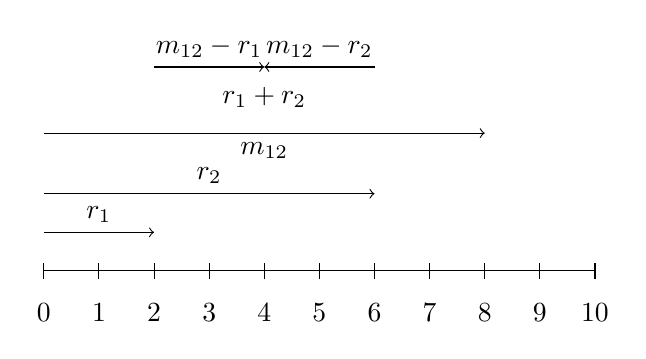
\begin{tikzpicture}[scale=.7]
\begin{scope}[yshift=-4mm]
\draw (0,0) -- (10,0);
\foreach \x in {0,1,...,10}
  \draw (\x,-1.5mm) -- +(0,3mm) node[below,yshift=-4mm] {$\x$};
\draw[->,yshift=7mm] (0,0) -- node[above] {$r_1$} (20mm,0);
\draw[->,yshift=14mm] (0,0) -- node[above] {$r_2$} (60mm,0);
\end{scope}
\draw[->,yshift=21mm] (0,0) -- node[above,yshift=2mm] {$r_1+r_2$} (80mm,0);
\coordinate (M) at (40mm,21mm);
\vertex{M};
\node[below] at (40mm,21mm) {$m_{12}$};
\begin{scope}[yshift=3mm]
\draw[->,yshift=30mm] (20mm,0mm) -- node[above] {$m_{12}-r_1$} +(20mm,0);
\draw[->,yshift=30mm] (60mm,0mm) -- node[above] {$m_{12}-r_2$} +(-20mm,0);
\end{scope}
\end{tikzpicture}
\end{center}
\caption{Relation between the roots $r_1,r_2=2,6$ and their average $m_{12}=4$}
\label{f.loh-roots1}
\end{figure}
If we use other values $r_1,r_2=3,5$ for which $r_1+r_2=8$ then $m_{12}=4$ remains the same while $s$ becomes $1$ (Fig.~\ref{f.loh-roots2}).

The offset $s$ seems to be arbitrary in:
\[
r_1=\left(\frac{-b}{2}+s\right)\,,\quad r_2=\left(\frac{-b}{2}-s\right)\,,
\]

\enlargethispage{\baselineskip}

\noindent{}but there is an additional constraint $r_1r_2=c$, where $c$ is the constant term in the polynomial.
By multiplying the two expressions we have derived for $r_1,r_2$, we can determine $s$ and then $r_1,r_2$:
\begin{eqnarray*}
c&=&\left(-\frac{b}{2} +s\right)\left(-\frac{b}{2} -s\right)=
  \frac{b^2}{4}-s^s\\
s&=&\frac{\sqrt{b^2-4c}}{2}\,.
\end{eqnarray*}

\begin{figure}[t]
\begin{center}
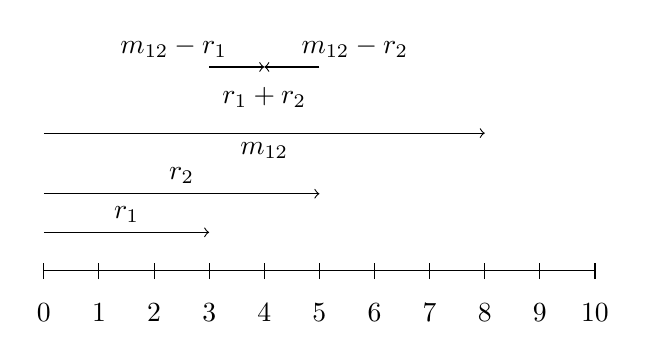
\begin{tikzpicture}[scale=.7]
\begin{scope}[yshift=-4mm]
\draw (0,0) -- (10,0);
\foreach \x in {0,1,...,10}
  \draw (\x,-1.5mm) -- +(0,3mm) node[below,yshift=-4mm] {$\x$};
\draw[->,yshift=7mm] (0,0) -- node[above] {$r_1$} (30mm,0);
\draw[->,yshift=14mm] (0,0) -- node[above] {$r_2$} (50mm,0);
\end{scope}
\draw[->,yshift=21mm] (0,0) -- node[above,yshift=2mm] {$r_1+r_2$}(80mm,0);
\coordinate (M) at (40mm,21mm);
\vertex{M};
\node[below] at (40mm,21mm) {$m_{12}$};
\begin{scope}[yshift=3mm]
\draw[->,yshift=30mm] (30mm,0mm) -- node[above left] {$m_{12}-r_1$} +(10mm,0);
\draw[->,yshift=30mm] (50mm,0mm) -- node[above right] {$m_{12}-r_2$} +(-10mm,0);
\end{scope}
\end{tikzpicture}
\end{center}
\caption{Relation between the roots $r_1,r_2=3,5$ and their average $m_{12}=4$}
\label{f.loh-roots2}
\end{figure}

\section{Examples of Loh's Method}\label{s.examples}

\begin{example}
Consider the polynomial  $x^2-2x-24$ where $b=-2,c=-24$:
\begin{eqnarray*}
c&=&\left(-\frac{(-2)}{2} +s\right)\left(-\frac{(-2)}{2} -s\right)\\
-24&=&(1 +s)(1 -s)\\
%s^2&=&25\\
s&=&5\\
r_1&=&1+5=6\\
r_2&=&1-5=-4\,.
\end{eqnarray*}
Check: $(x-6)(x-(-4))= x^2-2x-24$.
\end{example}

\begin{example}
Let us find the roots of $x^2-83x-2310$:
\begin{eqnarray*}
%c&=&\left(-\frac{b}{2} +s\right)\left(-\frac{b}{2} -s\right)\\
-2310&=&\left(\frac{83}{2}+s\right)\left(\frac{83}{2} -s\right)\\
s^2&=&\frac{6889}{4}+2310=\frac{16129}{4}\\
s&=&\frac{127}{2}\\
r_1&=&\frac{83}{2}-\frac{127}{2}=-22\\
r_2&=&\frac{83}{2}+\frac{127}{2}=105\,.
\end{eqnarray*}
Check: $(x+22)(x-105)= x^2-83x-2310$.

\newpage

Compare this computation with the computation using the traditional  formula:
\begin{eqnarray*}
\frac{-b\pm\sqrt{b^2-4c}}{2}&=&\frac{-(-83)\pm\sqrt{(-83)^2-4\cdot (-2310)}}{2}\\
%&=& \frac{83\pm\sqrt{6889+9240}}{2} = \frac{83\pm\sqrt{16129}}{2}\\
&=& \frac{83\pm\sqrt{16129}}{2} = \frac{83\pm 127}{2}\\
r_1&=&\frac{83-127}{2}=-22\\
r_2&=&\frac{83+127}{2}=105\,.
\end{eqnarray*}
\end{example}

\begin{example}
Theorem~\ref{thm.roots-coefficients} can be generalized to polynomials of higher degrees. Here is an interesting example for a \emph{quartic equation}\index{Quartic equation} $x^4-10x^2-x+20=0$. As with quadratic equations there are formulas for solving cubic and quartic equations (though not equations of higher powers), but the formulas are quite complicated.

Does this polynomial of degree four factor into two quadratic polynomials with integer coefficients? If so, the coefficients of the $x$ terms must be \emph{equal and of opposite signs} since the coefficient of the $x^3$ term is zero. Therefore, the form of the quadratic factors is:
\[
f(x) = (x^2 - nx + k_1)\, (x^2 + nx + k_2)\,.
\]
Carrying out the multiplication results in:
\[
\renewcommand{\arraystretch}{1.1}
\begin{array}{rrrrrr}
f(x) = &x^4 & + nx^3 & + k_2 x^2\\
&& -nx^3 &- n^2x^2 &-nk_2x\\
&&&+k_1x^2 &+ nk_1x &+ k_1k_2\,.
\end{array}
\]
Equating the coefficients gives three equations in the three unknowns $n,k_1,k_2$ gives:
\begin{eqnarray*}
(k_1+k_2)-n^2 &=& -10\\
n(k_1-k_2) &=& -1\\
k_1k_2 &=& 20\,.
\end{eqnarray*}
Since we are looking for factors with integer coefficients, from the last two equations it is clear that:
\[
n=1,\,k_1=4,\,k_2=5  \quad\quad\textrm{or} \quad\quad n=1,\,k_1=-5,\, k_2=-4\,.
\]
Only $n=1,k_1=-5,\, k_2=-4$ satisfy the first equation for the coefficient of $x^2$:
\[
f(x) = (x^2 - x - 5)\, (x^2 + x - 4)\,.
\]

\newpage

Solving these quadratic equations gives four solutions of the quartic equation:
\[
x = \frac{1\pm\sqrt{21}}{2}  \;\;\textrm{or} \;\; x= \frac{-1\pm\sqrt{17}}{2} \,.
\]
\end{example}

\section{Derivation of the Traditional Formula}\label{s.general}
\index{Quadratic equation!traditional formula}
For an arbitrary monic polynomial $x^2+bx+c$, Loh's formulas are:
\begin{eqnarray*}
c=r_1r_2&=&\left(\frac{-b}{2}+s\right)  \left(\frac{-b}{2}-s\right)=\left(\frac{b^2}{4}-s^2\right)\\
s&=&\sqrt{\left(\frac{b^2}{4}\right)-c}\\
r_1,r_2&=&\frac{-b}{2}\pm\sqrt{\left(\frac{b^2}{4}\right)-c}=\frac{-b\pm\sqrt{b^2-4c}}{2}\,,
\end{eqnarray*}
the traditional formula for obtaining the roots of a monic\index{Monic polynomial} quadratic polynomial. If the polynomial is not monic divide it by $a$, substitute in the  equation and simplify:
\begin{eqnarray*}
%ax^2+bx+c&=&0\\
x^2+\frac{b}{a}x+\frac{c}{a}&=&0\\
r_1,r_2&=&\frac{-(b/a)\pm\sqrt{(b/a)^2-4(c/a)}}{2}\\
%&=&\frac{-(b/a)\pm\sqrt{(b/a)^2-4(ac/a^2)}}{2}\\
&=&\frac{-b\pm\sqrt{b^2-4ac}}{2a}\,.
\end{eqnarray*}

\section{Al-Khwarizmi's Geometric Solution of Quadratic Equations}\label{s.khwar}

Let us write a monic\index{Monic polynomial} quadratic polynomial as $x^2+bx-c$. The roots can be found by \emph{completing the square}\index{Quadratic equation!completing the square}:
\begin{eqnarray*}
%x^2+bx&=&c\\
x^2+2\left(\frac{b}{2}\right)x+\left(\frac{b}{2}\right)^2&=&c+\left(\frac{b}{2}\right)^2\\
\left(x+\frac{b}{2}\right)^2&=&c+\left(\frac{b}{2}\right)^2\\
x&=&-\frac{b}{2}\pm\sqrt{c+\left(\frac{b}{2}\right)^2}=
\frac{-b\pm\sqrt{b^2+4c}}{2}\,.
\end{eqnarray*}
This is the familiar formula for finding the roots of a quadratic equation, except that $4c$ has the opposite sign since the  coefficient of the constant term was $-c$.

Completing the square was developed in the $8$th century by Muhammad ibn Musa al-Khwarizmi in a geometric context. Given the equation $x^2+bx=c$, assume that there is a square whose side is 
$x$ so that its area is $x^2$.
To the area $x^2$ add $bx$ by adding four rectangles of area $bx/4$ whose sides are $b/4$ and $x$ (Fig.~\ref{f.khw-1}). Now complete the diagram to a square by adding the four little squares of area $(b/4)^2$ (Fig.~\ref{f.khw-2}).

\begin{figure}[b]
\subfigures
\leftfigure[c]{
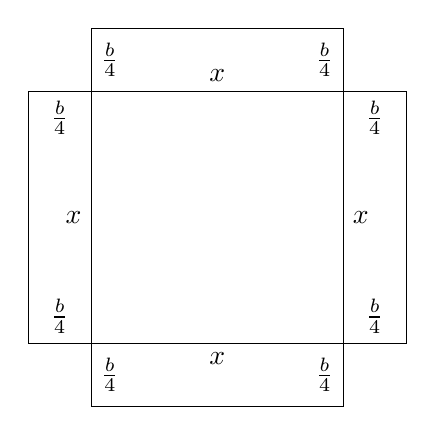
\begin{tikzpicture}[scale=.8]
\coordinate (A) at (0,0);
\coordinate (B) at (4,0);
\coordinate (C) at (4,4);
\coordinate (D) at (0,4);
\draw (A) -- node[below] {$x$} (B) -- node[right] {$x$} (C) -- node[above] {$x$} (D) -- node[left] {$x$} cycle;
\draw (A) -- node[right] {$\frac{b}{4}$} ++(0,-1) -- ++(4,0) -- node[left] {$\frac{b}{4}$} ++(0,1);
\draw (B) -- node[above] {$\frac{b}{4}$} ++(1,0) -- ++(0,4) -- node[below] {$\frac{b}{4}$} ++(-1,0);
\draw (C) -- node[left] {$\frac{b}{4}$} ++(0,1) -- ++(-4,0) -- node[right] {$\frac{b}{4}$} ++(0,-1);
\draw (D) -- node[below] {$\frac{b}{4}$} ++(-1,0) -- ++(0,-4) -- node[above] {$\frac{b}{4}$} ++(1,0);
\end{tikzpicture}
}
\hfill
\rightfigure[c]{
\begin{tikzpicture}[scale=.8]
\coordinate (A) at (0,0);
\coordinate (B) at (4,0);
\coordinate (C) at (4,4);
\coordinate (D) at (0,4);
\draw (A) -- node[below] {$x$} (B) -- node[right] {$x$} (C) -- node[above] {$x$} (D) -- node[left] {$x$} cycle;
\draw (A) -- node[right] {$\frac{b}{4}$} ++(0,-1) -- ++(4,0) -- node[left] {$\frac{b}{4}$} ++(0,1);
\draw (B) -- node[above] {$\frac{b}{4}$} ++(1,0) -- ++(0,4) -- node[below] {$\frac{b}{4}$} ++(-1,0);
\draw (C) -- node[left] {$\frac{b}{4}$} ++(0,1) -- ++(-4,0) -- node[right] {$\frac{b}{4}$} ++(0,-1);
\draw (D) -- node[below] {$\frac{b}{4}$} ++(-1,0) -- ++(0,-4) -- node[above] {$\frac{b}{4}$} ++(1,0);
\draw[thick,dashed] ($(A)+(0,-1)$) -- ++(-1,0) -- ++(0,1);
\draw[thick,dashed] ($(B)+(0,-1)$) -- ++(1,0) -- ++(0,1);
\draw[thick,dashed] ($(C)+(0,1)$) -- ++(1,0) -- ++(0,-1);
\draw[thick,dashed] ($(D)+(0,1)$) -- ++(-1,0) -- ++(0,-1);
\end{tikzpicture}
}
\leftcaption{The area is $x^2+4(b/4)x=x^2+bx$}\label{f.khw-1}
\rightcaption{The area is $x^2+4(b/4)x+4(b/4)^2=x^2+bx+(b^2/4)$}\label{f.khw-2}
\end{figure}

We can't construct the diagram in Fig.~\ref{f.khw-1} because we don't know what $x$ is, but the area of the larger square in  Fig.~\ref{f.khw-2} is:
\[
x^2+bx+\frac{b^2}{4}=c+\frac{b^2}{4}\,,
\]
which we do know since we are given the coefficients $b,c$. By constructing the diagram and erasing the small squares whose sides are $(b/4)$---another known quantity---we obtain the line segment of length $x$.

\begin{example}
Let $x^2+12x=64$. Then $c+(b^2/4)=64+36=100$. It is easy to construct a square of area $100$ since each side has length $10$. Now subtract $(b/4)+(b/4)=6$, the sides of the smaller squares, to get $x=10-6=4$.
\end{example}

\section{Cardano's Construction for Solving Cubic Equations}\label{s.cardano}

The formula for the roots of cubic equations\index{Cubic equation} was first published in the $16$th century by Gerolamo Cardano\index{Cardano, Gerolamo}. We will not develop the formula here, but it is interesting that the central idea is based on a geometric construction similar to al-Khwarizmi's. The construction can be obtained very simply using algebra. By multiplication:
\begin{align}\label{eq.car}
(a+b)^3=a^3+3a^2b+3ab^2+b^3=(a^3+b^3)+3ab(a+b)\,.
\end{align}
Geometrically, we start with a cube whose side is $a+b$ so that its volume is $(a+b)^3$. The cube is decomposed into five pieces. The first two are cubes whose sides are $a$ and $b$ with volumes $a^3$ (blue) and $b^3$ (red), respectively (Fig.~\ref{f.cardano1}).

The other three parts are boxes (the technical term is \emph{cuboid}) each with one side of length $a+b$ coinciding with a side of the cube, one side of length $a$ and one side of length $b$, so that the volume of each of the three boxes is $ab(a+b)$. In Fig.~\ref{f.cardano2}, there is one box at the left side of the cube (blue), one at the back of the cube (red) and one at the top of the cube (green).
By combining the five solids in Fig.~\ref{f.cardano1} and Fig.~\ref{f.cardano2} we obtain Eq.~\ref{eq.car}.


\begin{figure}[htb]
\begin{center}
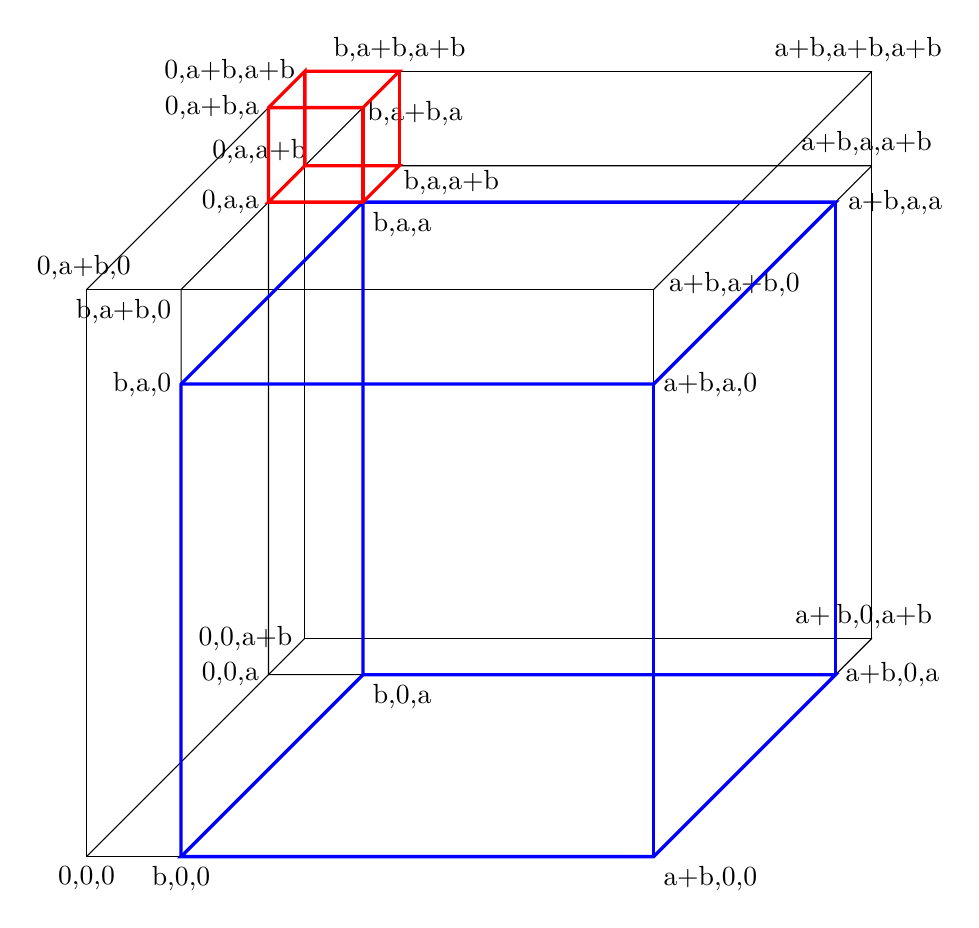
\begin{tikzpicture}[scale=1.2]

% Front face
\coordinate (A) at (0,0,0);
\node[below] at (A) {\sm{0,0,0}};
\coordinate (B) at (6,0,0);
\node[below right] at (B) {\sm{a+b,0,0}};
\coordinate (C) at (6,6,0);
\node[above right,xshift=2pt,yshift=-6pt] at (C)
  {\sm{a+b,a+b,0}};
\coordinate (D) at (0,6,0);
\node[above,xshift=-1pt] at (D) {\sm{0,a+b,0}};

% Front face
\coordinate (FF1) at (1,0,0);
\node[below] at (FF1) {\sm{b,0,0}};
\coordinate (FF2) at (1,5,0);
\node[left] at (FF2) {\sm{b,a,0}};
\coordinate (FF3) at (1,6,0);
\node[below left] at (FF3) {\sm{b,a+b,0}};
\coordinate (FF4) at (6,5,0);
\node[right] at (FF4) {\sm{a+b,a,0}};

% Back face
\coordinate (A1) at (0,0,-6);
\node[left,xshift=-1pt] at (A1) {\sm{0,0,a+b}};
\coordinate (B1) at (6,0,-6);
\node[above,xshift=-3pt] at (B1) {\sm{a+\:b,0,a+b}};
\coordinate (C1) at (6,6,-6);
\node[above,xshift=-5pt] at (C1) {\sm{a+b,a+b,a+b}};
\coordinate (D1) at (0,6,-6);
\node[left] at (D1) {\sm{0,a+b,a+b}};

% Back face
\coordinate (BF1) at (0,5,-6);
\node[above left,xshift=4pt,yshift=-3pt] at (BF1) 
  {\sm{0,a,a+b}};
\coordinate (BF2) at (1,5,-6);
\node[below right,xshift=-2pt,yshift=2pt] at (BF2)
  {\sm{b,a,a+b}};
\coordinate (BF3) at (1,6,-6);
\node[above] at (BF3) {\sm{b,a+b,a+b}};
\coordinate (BF4) at (6,5,-6);
\node[above,xshift=-2pt] at (BF4) {\sm{a+b,a,a+b}};

% Right face
\coordinate (RF1) at (6,5,-5);
\node[right,xshift=1pt] at (RF1) {\sm{a+b,a,a}};
\coordinate (RF2) at (6,0,-5);
\node[right] at (RF2) {\sm{a+b,0,a}};

% Bottom face
\coordinate (BT1) at (1,0,-5);
\node[below right] at (BT1) {\sm{b,0,a}};

% Left face
\coordinate (LF1) at (0,0,-5);
\node[left] at (LF1) {\sm{0,0,a}};
\coordinate (LF2) at (0,5,-5);
\node[left] at (LF2) {\sm{0,a,a}};
\coordinate (LF3) at (0,6,-5);
\node[left] at (LF3) {\sm{0,a+b,a}};

% Top face
\coordinate (TF1) at (1,6,-5);
\node[right,xshift=-2pt,yshift=-2pt] at (TF1) {\sm{b,a+b,a}};

% Internal point
\coordinate (I) at (1,5,-5);
\node[below right] at (I) {\sm{b,a,a}};


\draw (A) -- (B) -- (C) -- (D) -- cycle;
\draw (A1) -- (B1) -- (C1) -- (D1) -- cycle;
\draw (A) -- (A1);
\draw (B) -- (B1);
\draw (C) -- (C1);
\draw (D) -- (D1);

\draw (FF1) -- (FF2) -- (FF3) -- (BF3);
\draw (BF2) -- (FF2) -- (FF4) -- (BF4);
\draw (FF1) -- (BT1) -- (TF1);
\draw (BF3) -- (BF2);
\draw (TF1) -- (LF3);
\draw (LF3) -- (LF1) -- (RF2) -- (RF1) -- (LF2) -- 
      (BF1) -- (BF4);

\draw[very thick,blue] (FF1) -- (B) -- (RF2) -- (BT1) -- cycle; 
\draw[very thick,blue] (FF1) -- (FF2) -- (I) -- (BT1);
\draw[very thick,blue] (I) -- (RF1) -- (FF4) -- (FF2);
\draw[very thick,blue] (FF4) -- (B);
\draw[very thick,blue] (RF1) -- (RF2);

\draw[very thick,red] (I) -- (LF2) -- (BF1) -- (BF2) -- cycle;
\draw[very thick,red] (LF2) -- (LF3) -- (D1) -- (BF1);
\draw[very thick,red] (D1) -- (BF3) -- (TF1) -- (LF3);
\draw[very thick,red] (TF1) -- (I);
\draw[very thick,red] (BF3) -- (BF2);

\end{tikzpicture}
\end{center}
\caption{$(a^3+b^3)=(a^3+b^3)+\cdots$}\label{f.cardano1}
\end{figure}

%%%%%%%%%%%%%%%%%%%%%%%%%%%%%%%%%%%%%%%%%%%%%%%%%%%%%%%%%%%%%

\begin{figure}[htb]
\begin{center}
\begin{tikzpicture}[scale=1.2]

% Front face
\coordinate (A) at (0,0,0);
\node[below] at (A) {\sm{0,0,0}};
\coordinate (B) at (6,0,0);
\node[below right] at (B) {\sm{a+b,0,0}};
\coordinate (C) at (6,6,0);
\node[above right,xshift=2pt,yshift=-6pt] at (C)
  {\sm{a+b,a+b,0}};
\coordinate (D) at (0,6,0);
\node[above,xshift=-1pt] at (D) {\sm{0,a+b,0}};

% Front face
\coordinate (FF1) at (1,0,0);
\node[below] at (FF1) {\sm{b,0,0}};
\coordinate (FF2) at (1,5,0);
\node[left] at (FF2) {\sm{b,a,0}};
\coordinate (FF3) at (1,6,0);
\node[below left] at (FF3) {\sm{b,a+b,0}};
\coordinate (FF4) at (6,5,0);
\node[right] at (FF4) {\sm{a+b,a,0}};

% Back face
\coordinate (A1) at (0,0,-6);
\node[left,xshift=-1pt] at (A1) {\sm{0,0,a+b}};
\coordinate (B1) at (6,0,-6);
\node[above,xshift=-3pt] at (B1) {\sm{a+\:b,0,a+b}};
\coordinate (C1) at (6,6,-6);
\node[above,xshift=-5pt] at (C1) {\sm{a+b,a+b,a+b}};
\coordinate (D1) at (0,6,-6);
\node[left] at (D1) {\sm{0,a+b,a+b}};

% Back face
\coordinate (BF1) at (0,5,-6);
\node[above left,xshift=4pt,yshift=-3pt] at (BF1) 
  {\sm{0,a,a+b}};
\coordinate (BF2) at (1,5,-6);
\node[below right,xshift=-2pt,yshift=2pt] at (BF2)
  {\sm{b,a,a+b}};
\coordinate (BF3) at (1,6,-6);
\node[above] at (BF3) {\sm{b,a+b,a+b}};
\coordinate (BF4) at (6,5,-6);
\node[above,xshift=-2pt] at (BF4) {\sm{a+b,a,a+b}};

% Right face
\coordinate (RF1) at (6,5,-5);
\node[right,xshift=1pt] at (RF1) {\sm{a+b,a,a}};
\coordinate (RF2) at (6,0,-5);
\node[right] at (RF2) {\sm{a+b,0,a}};

% Bottom face
\coordinate (BT1) at (1,0,-5);
\node[below right] at (BT1) {\sm{b,0,a}};

% Left face
\coordinate (LF1) at (0,0,-5);
\node[left] at (LF1) {\sm{0,0,a}};
\coordinate (LF2) at (0,5,-5);
\node[left] at (LF2) {\sm{0,a,a}};
\coordinate (LF3) at (0,6,-5);
\node[left] at (LF3) {\sm{0,a+b,a}};

% Top face
\coordinate (TF1) at (1,6,-5);
\node[right,xshift=-2pt,yshift=-2pt] at (TF1) {\sm{b,a+b,a}};

% Internal point
\coordinate (I) at (1,5,-5);
\node[below right] at (I) {\sm{b,a,a}};


\draw (A) -- (B) -- (C) -- (D) -- cycle;
\draw (A1) -- (B1) -- (C1) -- (D1) -- cycle;
\draw (A) -- (A1);
\draw (B) -- (B1);
\draw (C) -- (C1);
\draw (D) -- (D1);

\draw (FF1) -- (FF2) -- (FF3) -- (BF3);
\draw (BF2) -- (FF2) -- (FF4) -- (BF4);
\draw (FF1) -- (BT1) -- (TF1);
\draw (BF3) -- (BF2);
\draw (TF1) -- (LF3);
\draw (LF3) -- (LF1) -- (RF2) -- (RF1) -- (LF2) -- 
      (BF1) -- (BF4);

\draw[very thick,blue] (A) -- (FF1) -- (FF3) -- (D) -- cycle;
\draw[very thick,blue] (FF1) -- (BT1) -- (TF1) -- (FF3);
\draw[very thick,blue] (TF1) -- (LF3) -- (D);
\draw[very thick,blue] (LF3) -- (LF1) -- (A);
\draw[very thick,blue] (LF1) -- (BT1);

\draw[very thick,red] (LF1) -- (RF2) -- (RF1) -- (LF2);
\draw[very thick,red] ($(LF2) + (2pt,0)$) -- ($(LF1) + (2pt,0)$);
\draw[very thick,red] (A1) -- (B1) -- (BF4) -- (BF1) -- cycle;
\draw[very thick,red] ($(LF2) + (2pt,0)$) -- ($(BF1) + (2pt,0)$);
\draw[very thick,red] (BF4) -- (RF1);
\draw[very thick,red] (B1) -- (RF2);
\draw[very thick,red] (A1) -- (LF1);

\draw[very thick,green] (FF2) -- (FF4) -- (C) -- (FF3);
\draw[very thick,green] 
  ($(FF2) + (2pt,0)$) -- ($(FF3) + (2pt,0)$);
\draw[very thick,green] 
  ($(FF4) + (0,2pt)$) -- ($(BF4) + (0,2pt)$);
\draw[very thick,green] (BF4) -- (C1) -- (BF3);
\draw[very thick,green] 
  ($(BF3) + (2pt,0)$) -- ($(FF3) + (2pt,0)$);
\draw[very thick,green] (C1) -- (C);
\draw[very thick,green] (BF3) -- (BF2) -- (FF2);
\draw[very thick,green] 
  ($(BF2) + (0,2pt)$) -- ($(BF4) + (0,2pt)$);


\end{tikzpicture}
\end{center}
\caption{$(a^3+b^3)=\cdots+3ab(a+b)$}\label{f.cardano2}
\end{figure}

\section{They Weren't Intimidated by Imaginary Numbers}\label{s.imaginary}

The history of mathematics demonstrates a progression of concepts that were initially considered to be meaningless, but were eventually understood, accepted and proved to be useful. ``Obviously,'' since numbers count things, $-1$, a negative number, is meaningless. ``Obviously,'' since numbers are ratios of integers (rational numbers), $\sqrt{2}$, which can easily be proved to be irrational, is meaningless. ``Obviously,'' $\sqrt{-1}$, the square root of a negative number, is meaningless since there is no number---integer, rational or real---whose square is $-1$.

A full understanding of the square roots of negative numbers, to this day called \emph{imaginary numbers} although they are no less real than real numbers, was not achieved until the nineteenth century. Therefore, it is surprising that already in the sixteenth century, Geralamo Cardano and Rafael Bombelli refused to be intimidated by the concept, and took the first small steps towards understanding these numbers.

Consider the quadratic equation:
\begin{align}
x^2-10x+40=0\,.\label{eq.cardano-quadratic}
\end{align}
By the familiar formula (Eq.~\ref{eq.quadratic-roots}):
\[
r_1, r_2=\displaystyle\frac{10\pm\sqrt{100-160}}{2}=5\pm\sqrt{-15}\,.
\]
Well, we don't know anything about the square roots of negative numbers and we don't know what these values are, but like Cardano we do know by Thm~\ref{eq.quadratic-roots} that:
\[
\begin{array}{lcl}
r_1+r_2&=&(5+\sqrt{-15})+(5-\sqrt{-15})=10=-b\\
r_1r_2&=&(5+\sqrt{-15})(5-\sqrt{-15})=25-5\sqrt{-15}+5\sqrt{-15}-(-15)=40=c\,.
\end{array}
\]
which correspond with the coefficients of the quadratic equation Eq.~\ref{eq.cardano-quadratic}. It is rather intuitive that $\sqrt{-15}+(-\sqrt{-15})=0$ even if we know nothing about $\sqrt{-15}$, and, similarly, it is rather intuitive that $\sqrt{-15}\cdot-(\sqrt{-15})=-(-15)=15$ even if we don't know what $\sqrt{-15}$ is.

\enlargethispage{\baselineskip}

Consider now the cubic equation:
\begin{align}
x^3-15x-4=0\,.\label{eq.bombelli-cubic}
\end{align}
It is not hard to observe that $4$ is a root, but how can it be computed? Cardano's formula gives the root:
\begin{align}
r=\sqrt[3]{2+11\sqrt{-1}}+\sqrt[3]{2-11\sqrt{-1}}\,,\label{eq.cube-root}
\end{align}
a quite complicated formula that bears no obviously relation to $4$. 

Bombelli courageously performed the following computation (see Eq.~\ref{eq.car}):
\begin{eqnarray*}
(2+\sqrt{-1})^3&=&
8+3\cdot 4\sqrt{-1}+3\cdot 2(-1)+(-1\sqrt{-1})=
2+11\sqrt{-1}\\
(2-\sqrt{-1})^3&=&
8-3\cdot 4\sqrt{-1}+3\cdot 2(-1)-(-1\sqrt{-1})=
2-11\sqrt{-1}\,,
\end{eqnarray*}
and by Eq.~\ref{eq.cube-root}:
\begin{eqnarray*}
r&=&\sqrt[3]{2+11\sqrt{-1}} + \sqrt[3]{2-11\sqrt{-1}}\\
&=&\sqrt[3]{(2+\sqrt{-1})^3} + \sqrt[3]{(2-\sqrt{-1})^3}\\
&=&(2+\sqrt{-1}) + (2-\sqrt{-1})=4\,.
\end{eqnarray*}


%%%%%%%%%%%%%%%%%%%%%%%%%%%%%%%%%%%%%%%%%%%%%%%%%%%%%%%%

\section{Lill's Method and Carlyle's Circle}\label{s.lill-quadratic}

Lill's method can be applied to solve quadratic equations.\footnote{This section assumes that you have read about Lill's method in Chap.~\ref{c.origami-cube}.}\index{Lill's method!quadratic equations} As an example we use Eq.~\ref{eq.quadratic-lill} which gives the roots of a quadratic equation obtained by factorization:
\[
x^2+bx+c=x^2-4x+3= (x-1)(x-3)\,.
\]
Applying Lill's method results in the paths shown in Fig.~\ref{f.lill-quadratic}.

\begin{figure}[bt]
\begin{center}
\begin{tikzpicture}[scale=1.1]
% Draw help lines and axes
\draw[step=10mm,white!50!black] (-4,-5) grid (2,1);
\draw[thick] (-4,0) -- (2,0);
\draw[thick] (0,-5) -- (0,1);
\foreach \x in {-3,...,2}
  \node at (\x-.2,.2) {\sm{\x}};
\foreach \y in {-4,...,-1}
  \node at (-.2,\y-.3) {\sm{\y}};

 Draw first path
\coordinate (A) at (0,0);
\coordinate (B) at (1,0);
\coordinate (C) at (1,-4);
\coordinate (D) at (-2,-4);
\draw[very thick] (A) --
  node[above] {$1$} (B);
\draw[very thick,name path=bc] (B) -- 
  node[right,xshift=-1pt,yshift=6pt] {$b=-4$} (C);
\draw[very thick,name path=cd] (C) --
  node[below left,xshift=3pt] {$c=3$}(D);

% Draw first segment of second path
\path[name path=a2] (A) -- +(-45:1.414);
\path [name intersections = {of = a2 and bc, by = {A2}}];
\node[above right] at (A2) {$P_1$};
\draw[very thick,dashed] (A) -- (A2);
\draw ($(A) + (14pt,0)$)
  arc [start angle=0, end angle = -45, radius=14pt];
\node[below right,xshift=40pt,yshift=-2pt] at (A) {$-45^\circ$};
\draw[->] ($(A)+(33pt,-6pt)$) -- +(-18pt,0);
\draw[rotate=135] (A2) rectangle +(5pt,5pt);

% Draw second segment of second path
\path[name path=b2] (A2) -- +(-135:5);
\path [name intersections = {of = b2 and cd, by = {B2}}];
\draw[very thick,dashed] (A2) -- (B2);

% Draw first segment of second path
\path[name path=a3] (A) -- +(-71.57:4);
\path [name intersections = {of = a3 and bc, by = {A3}}];
\node[above right] at (A3) {$P_2$};
\draw[very thick,dashed] (A) -- (A3);
\draw ($(A) + (20pt,0)$)
  arc [start angle=0, end angle = -71.57, radius=20pt];
\node[below right,xshift=40pt,yshift=-10pt] at (A) {$-71.57^\circ$};
\draw[->] ($(A)+(35pt,-13pt)$) -- +(-18pt,0);
\draw[rotate=108.43] (A3) rectangle +(5pt,5pt);

% Draw second segment of second path
\path[name path=b3] (A3) -- +(198.43:5);
\path [name intersections = {of = b3 and cd, by = {B3}}];
\draw[very thick,dashed] (A3) -- (B3);

\end{tikzpicture}
\end{center}
\caption{Lill's method on $x^2-4x+3$}\label{f.lill-quadratic}
\end{figure}
Check that the angles are correct:
\[
-\tan (-45^\circ) = -1,\quad -\tan (-71.57^\circ) \approx -3\,.
\]
For quadratic equations we can find the points $P_1,P_2$ as the intersections of the line representing the coefficient $b$ and the circle whose diameter is the line connecting the starting point and the end point of the paths (Fig.~\ref{f.lill-circle}). In order for a point on the line $b$ to be a root, the reflection of the line must be $90^\circ$ and therefore the inscribed angle is subtended by a diameter.

\begin{figure}[t]
\begin{center}
\begin{tikzpicture}[scale=1]
% Draw help lines and axes
\draw[step=10mm,white!50!black] (-4,-5) grid (2,1);
\draw[thick] (-4,0) -- (2,0);
\draw[thick] (0,-5) -- (0,1);
\foreach \x in {-3,...,2}
  \node at (\x-.2,.2) {\sm{\x}};
\foreach \y in {-4,...,-1}
  \node at (-.2,\y-.3) {\sm{\y}};

 Draw first path
\coordinate (A) at (0,0);
\coordinate (B) at (1,0);
\coordinate (C) at (1,-4);
\coordinate (D) at (-2,-4);
\draw[very thick] (A) --
  node[above] {$1$} (B);
\draw[very thick,name path=bc] (B) -- 
  node[right,xshift=-2pt,yshift=6pt] {$b=-4$} (C);
\draw[very thick,name path=cd] (C) --
  node[below left,xshift=-1pt,yshift=-5pt] {$c=3$}(D);

% Draw first segment of second path
\path[name path=a2] (A) -- +(-45:1.414);
\path [name intersections = {of = a2 and bc, by = {A2}}];
\node[above right] at (A2) {$P_1$};
\draw[dashed] (A) -- (A2);
\draw ($(A) + (14pt,0)$)
  arc [start angle=0, end angle = -45, radius=14pt];
\node[below right,xshift=40pt,yshift=-2pt] at (A) {$-45^\circ$};
\draw[->] ($(A)+(33pt,-6pt)$) -- +(-18pt,0);
\draw[rotate=135] (A2) rectangle +(5pt,5pt);

% Draw second segment of second path
\path[name path=b2] (A2) -- +(-135:5);
\path [name intersections = {of = b2 and cd, by = {B2}}];
\draw[dashed] (A2) -- (B2);

% Draw first segment of second path
\path[name path=a3] (A) -- +(-71.57:4);
\path [name intersections = {of = a3 and bc, by = {A3}}];
\node[above right] at (A3) {$P_2$};
\draw[dashed] (A) -- (A3);
\draw ($(A) + (20pt,0)$)
  arc [start angle=0, end angle = -71.57, radius=20pt];
\node[below right,xshift=40pt,yshift=-10pt] at (A) {$-71.57^\circ$};
\draw[->] ($(A)+(35pt,-13pt)$) -- +(-18pt,0);
\draw[rotate=108.43] (A3) rectangle +(5pt,5pt);

% Draw second segment of second path
\path[name path=b3] (A3) -- +(198.43:5);
\path [name intersections = {of = b3 and cd, by = {B3}}];
\draw[dashed] (A3) -- (B3);

\coordinate (O) at (-1,-2);
\vertex{O};
\node[draw,circle through=(A)] at (O) {};
\draw[very thick,dotted] (A) -- (D);

\end{tikzpicture}
\end{center}
\caption{Constructing a circle to find the roots}\label{f.lill-circle}
\end{figure}

This can also be checked by computation. The center of the circle is the midpoint of the diameter $(-1,-2)$. The length of the diameter is:
\[
\sqrt{(-2)^2+(-4)^2}=\sqrt{20}\,,
\]
so the square of the length of the radius is $\left(\sqrt{20/2}\right)^2=5$. We need the intersection of this circle and the line $x=1$:
\begin{eqnarray*}
(x-(-1))^2+(y-(-2))^2&=&r^2\\
(x^2+2x+1)+(y^2+4y+4)&=&5\\
y^2+4y+3&=&0\\
y&=&-1,\;-3\,.
\end{eqnarray*}


A similar method for solving quadratic equations is the Carlyle circle\index{Carlyle circle} which predates Lill's method. Given a quadratic equation $x^2-bx+c$ (note the minus sign on the linear term), construct points at $(0,1)$ and $(b,c)$. Construct a circle whose diameter is the line connecting the two points (Fig.~\ref{f.carlyle-circle}). Its intersections (if any) with the $x$-axis are the roots of the equation.

In the general case, the center of the circle is $(b/2,(c-(-1))/2)$ and the length of the diameter is $\sqrt{b^2+(c-1)^2}$, so the equation of the circle is:
\[
\left(x-\frac{b}{2}\right)^2+\left(y-\frac{c+1}{2}\right)^2=
\frac{b^2+(c-1)^2}{4}\,.
\]
For the example, substituting $b=4,c=3$ and $y=0$, we see that  $x=1$ and $x=3$ are the roots of the quadratic equation.


\begin{figure}[t]
\begin{center}
\begin{tikzpicture}[scale=1]
% Draw help lines and axes
\draw[step=10mm,white!50!black] (-1,-1) grid (5,5);
\draw[thick] (-1,0) -- (5,0);
\draw[thick] (0,-1) -- (0,5);
\foreach \x in {0,...,5}
  \node at (\x-.2,.2) {\sm{\x}};
\foreach \y in {1,...,4}
  \node at (-.1,\y+.2) {\sm{\y}};

\coordinate (A) at (0,1);
\node[below left] at (A) {$(0,1)$};
\coordinate (B) at (4,3);
\node[above right] at (B) {$(4,3)$};
\vertex{A};
\vertex{B};

\coordinate (O) at (2,2);
\vertex{O};
\node[draw,circle through=(B)] at (O) {};
\draw[very thick,dotted] (A) -- (B);

\coordinate (X1) at (1,0);
\node[below left] at (X1) {$(1,0)$};
\coordinate (X2) at (3,0);
\node[below right] at (X2) {$(3,0)$};
\vertex{X1};
\vertex{X2};

\end{tikzpicture}
\end{center}
\caption{Carlyle circle for $x^2-4x+3$}\label{f.carlyle-circle}
\end{figure}


\section{Numerical Computation of the Roots}\label{s.numerical}
\index{Quadratic equation!numerical computation of the roots}

Students learn symbolic computation of roots, derivatives and so on. Today, most computation is performed by computers so symbolic computation is less important. \emph{Numerical analysis} is the branch of mathematics and computer science that develops accurate and efficient computational methods. The main challenge is to deal with the finiteness of values stored in the computer's memory. The computation:
\[0.12\times 0.14=0.0168\]
is easy to do, but:
\[
0.123456789\times 0.123456789\]
needs eighteen digits to be accurately represented and this cannot be done in a memory word that stores sixteen digits. This error is called a \emph{round-off error}.\index{Round-off error}

An even more serious problem is encountered when \emph{floating point arithmetic} is performed. Clearly:
\[(0.12\times 10^{-10})\times (0.14\times 10^{-8})\]
would not be computed by writing out all the zero digits. Instead, we multiply the mantissas and add the exponents to obtain $0.0168\times 10^{-18}$, which is normalized to $0.168\times 10^{-19}$ so that the most significant digit appears after the decimal point, ensuring maximum precision given the fixed size of the mantissa. If the maximum exponent that can be represented is $-16$ the result simply cannot even be stored. This error is called \emph{floating-point underflow}.\index{Floating-point underflow}

\newpage

The formula for finding the roots of the quadratic equation $x^2+bx+c$ is:
\begin{align}
r_1, r_2 = \frac{-b\pm\sqrt{b^2-4c}}{2}\,.\label{eq.quadratic-numerical}
\end{align}
Consider what happens if $b=1000$ and $c=4$. The roots are:
\[
r_1, r_2 = \frac{-1000\pm\sqrt{1000000-16}}{2}\,.
\]
Depending on the precision of the arithmetic, it is possible that one of the roots is so close to zero that the value stored is zero. Evaluating the quadratic equation gives the surprising result $0^2+b\cdot 0 +4= 4= 0$.

Can we do better? By Eq.~\ref{eq.viete-quad}:
\[
r_1+r_2 = -b\,,\quad\quad r_1r_2=c\,.
\]
If $r_2$ is much less that $r_1$, written $r_2\ll r_1$, then $r_1\approx -b$ and $r_2=c/b$. Table~\ref{t.quadratic}, computed by a computer program, compares the values of the roots computed by these formulas with the values obtained from the traditional formula Eq.~\ref{eq.quadratic-numerical}. The value of $c$ is fixed at $4$ and the roots for increasing values of $b$ are shown.

Initially, the true values computed by the traditional formula for $r_2$ are more accurate ($r_2-r_{2v}$ is negative) but from $b=100000$, the computation based upon Eq.~\ref{eq.viete-quad} is more accurate. Such are the surprises of numerical analysis.

\begin{table}[bht]
\caption[Two computations of the roots of a quadratic equation]{Two computations of the roots of a quadratic equation. $r_1,r_2$ are the roots computed by Eq.~\ref{eq.quadratic-numerical}. $r_{1v},r_{2v}$ are the roots computed using Eq.~\ref{eq.viete-quad}. The errors are $r_{i}-r_{iv}$. The values are truncated to four decimal places.
Floating-point numbers are written $-4e-5$ in place of $4\times 10^{-5}$ because computer programs are normally written as linear sequences of characters.} \label{t.quadratic}
\[
\begin{array}{r@{\hspace{2.5mm}}r@{\hspace{2.5mm}}r@{\hspace{2.5mm}}r@{\hspace{2.5mm}}r@{\hspace{2.5mm}}r@{\hspace{2.5mm}}r}
\hline
\noalign{\smallskip}
b & r_1 & r_{1v} & \mathrm{Error}_1 & r_2 & r_{2v} & \mathrm{Error}_2\\
\noalign{\smallskip}\svhline\noalign{\smallskip}
100  &  -99.9599  &  -100  &  0.0400  &  -0.04001\  &  -0.04  &  -1.6012e\!-\!05\\
1000  &  -999.9959  &  -1000  &  0.0040  &  -0.0040  &  -0.004  &  -1.6000e\!-\!08\\
10000  &  -9999.9996  &  -10000  &  0.0004  &  -0.0004  &  -0.0004  &  -1.6270e\!-\!11\\
100000  &  -99999.9999  &  -100000  &  3.9999e\!-\!5  &  -3.9999e\!-\!5  &  -4e\!-\!5  &  1.0104e\!-\!12\\
1000000  &  -999999.9999  &  -1000000  &  4.0000e\!-\!6  &  -3.9999e\!-\!6  &  -4e\!-\!6  &  2.7749e\!-\!11\\
10000000  &  -10000000.0  &  -10000000  &  3.9860e\!-\!7  &  -3.9953e\!-\!7  &  -4e\!-\!7  &  4.6261e\!-\!10\\
 \noalign{\smallskip}
 \hline
\end{array}
\]
\end{table}

\newpage

\subsection*{What Is the Surprise?}

Poh-Shen Loh's approach provides a new way of looking at the relation between the coefficients and the roots that one doesn't see simply by memorizing the traditional formula. What is surprising is that this relation is fundamental in Gauss's algebraic proof of the constructibility of a regular heptadecagon (Chap.~\ref{c.heptadecagon}).

With the modern dominance of algebraic methods in geometry it is important to be reminded that the reverse once held. As shown by the constructions of Al-Khwarizmi and Cardano, geometric methods were used to obtain results in algebra. Lill and Carlyle both developed geometric methods for solving quadratic equations. Considerations of numerical computation on computers will surprise students who have not experienced it before.

\subsection*{Sources}
Poh-Shen Loh's method is from \cite{loh1,loh2}. Al-Khwarizmi's construction is from \cite[Chapter~1]{jorg} and \cite{mastin}. Cardano's construction can be found in \cite[Chap.~1]{jorg}. For the colorful history of the development of Cardano's formula see \cite{wiki:cardano}. The early attempts at computing with imaginary numbers are from \cite[Chapter~2]{jorg}. Lill's method and Carlyle's circle can be found in \cite{wiki:quadratic} together with a discussion of numerical computation of the roots.



\tikzsetfigurename{induction}
% !TeX Program=XeLaTeX
% !TeX root = surprises.tex

\selectlanguage{hebrew}

\chapter{אינדוקציה}\label{c.induction}

%%%%%%%%%%%%%%%%%%%%%%%%%%%%%%%%%%%%%%%%%%%%%%%%%%%%%%%%%%%%%%%

האקסיומה של אינדוקציה מתמטית נמצאת בשימוש נרחב כשיטת הוכחה במתמטיקה. פרק זה מציג הוכחות אינדוקטיביות של תוצאות שייתכן שאינן מוכרות לקורא. נתחיל בסקירה קצרה של אינדוקציה מתמטית (סעיף%
~\ref{s.induction-axiom}).
סעיף%
~\ref{s.induction-fibonacci}
מביא הוכחות של משפטים על מספרי פיבונאצ'י
\L{(Fibonacci)}
המוכרים וסעיף%
~\ref{s.induction-fermat}
מביא הוכחות של משפטים על מספרי פרמה
\L{(Fermat)}.
בסעיף%
~\ref{s.induction-mccarthy}
נציג את פונקציה
$91$
של ג'ון מקארתי
\L{(John McCarthy)}.
ההוכחה אינה שגרתית כי היא משתמשת באינדוקציה על מספרים שלמים בסדר הפוך. הוכחת הנוסחה עבור הבעיה של יוסף בן-מתתיהו
\L{(Josephus)}
גם היא אינה שגרתית כי היא משתמשת באינדוקציה כפולה על חלקים שונים של ביטוי (סעיף%
.~\ref{s.josephus}).

\section{האקסיומה של אינדוקציה מתמטית}\label{s.induction-axiom}

אינדוקציה מתמטית היא הדרך המובילה להוכחת משפטים עבור קבוצה לא חסומה של מספרים. נעיין בשוויונות:
\[
1=1,\quad 1+2=3,\quad 1+2+3=6,\quad 1+2+3+4=10\,,
\]
נשים לב ש:
\[
1=(1\cdot 2)/2,\quad 3=(2\cdot 3)/2,\quad  6=(3\cdot 4)/2,\quad 10=(4\cdot 5)/2\,,
\]
ונשער שעבור כל המספרים שלמים
$n\geq 1$:
\[
\sum_{i=1}^n i = \frac{n(n+1)}{2}\,.
\]
עם מספיק סבלנות קל לבדוק את הנוסחה עבור כל ערך מסוים של
$n$,
אבל איך אפשר להוכיח עבור אינסוף המספרים השלמים החיוביים? כאן נכנסת אינדוקציה מתמטית.

\begin{axiom}
תהי
$P(n)$
תכונה (כגון משוואה, נוסחה או משפט), כאשר 
$n$
הוא מספר שלם חיובי. נניח שניתן:
\begin{itemize}
\item \textbf{טענת הבסיס}: 
להוכיח ש-%
$P(1)$
נכונה,
\item \textbf{צעד אינדוקטיבי}:
עבור 
$m$
שרירותי, להוכיח ש-%
$P(m+1)$
נכונה בהנחה ש-%
$P(m)$
נכונה,
\end{itemize}
אז
$P(n)$
נכונה עבור כל
$n\geq 1$.
ההנחה ש-%
$P(m)$
נכונה עבור 
$m$ 
שרירותי נקראת
\textbf{הנחת האינדוקציה}.
\end{axiom}

הנה דוגמה פשוטה עבור הוכחה באינדוקציה מתמטית.
\begin{theorem}\label{t.sum}
עבור
$n\geq 1$:
\[
\sum_{i=1}^n i = \frac{n(n+1)}{2}\,.
\]
\end{theorem}

\begin{proof} 
טענת הבסיס פשוטה:
\[
\sum_{i=1}^1 i = 1 =\frac{1(1+1)}{2}\,.
\]
הנחת האינדוקציה היא שמשוואה שלהלן נכונה עבור  
$m$:
\[
\sum_{i=1}^{m} i = \frac{m(m+1)}{2}\,.
\]
הצעד האינדוקטיבי הוא להוכיח את המשפט עבור
$m+1$:
\begin{eqn}
\sum_{i=1}^{m+1} i &=& \sum_{i=1}^m i + (m+1)\label{l.sum1}\\
&=&\frac{m(m+1)}{2} + (m+1)\label{l.sum2}
%&=&\frac{m(m+1) + 2(m+1)}{2}\label{l.sum3}\\
=\frac{(m+1)(m+2)}{2}\,.\label{l.sum4}
\end{eqn}
לפי אקסיומת האינדוקציה המתמטית, עבור כל
$n\geq 1$:
\[
\sum_{i=1}^n i = \frac{n(n+1)}{2}\,.
\]
\end{proof}

הנחת האינדוקציה עלולה לבלבל ,כי נראה שאנחנו מניחים את מה שרוצים להוכיח. אין כאן הסקת מסקנות מעגלית כי ההנחה היא עבור תכונה של משהו קטן ומשתמשים בהנחה כדי להוכיח תכונה עבור משהו גדול יותר.

אינדוקציה מתמטית היא אקסיומה שאי-אפשר להוכיח. פשוט צריכים לקבל אותה כמו שמקבלים אקסיומות אחרות כגון
$x+0=x$.
כמובן שתוכלו לדחות את האקסיומה, אבל אז תצטרכו לדחות חלק גדול מהמתמטיקה המודרנית.
\begin{advanced}
אינדוקציה מתמטית היא כלל היסק שהוא אחד מאקסיומות פאנו
\L{(Peano)}
לפורמליזציה של המספרים הטבעיים. ניתן להוכיח את האקסיומה בעזרת אקסיומה אחרת כגון עקרון הסדר הטוב
ולהפך, אבל לא ניתן להוכיח אותה בעזרת אקסיומות אחרות, פשוטות יותר, של פאנו. 
\end{advanced}

%%%%%%%%%%%%%%%%%%%%%%%%%%%%%%%%%%%%%%%%%%%%%%%%%%%%%%%%


\section{מספרי פיבונאצ'י }\label{s.induction-fibonacci}

מספרי פיבונטצ'י מוגדרים ברקורסיה:
\begin{eqn}
f_1 &=& 1\\
f_2 &=& 1\\
f_n &=& f_{n-1} + f_{n-2}, \;\;  n \geq 3 \;\; \textrm{\R{עבור}}\,.
\end{eqn}
שנים עשר מספרי פיבונאצ'י הראשונים הם:
$
1, 1, 2, 3, 5, 8, 13, 21, 34, 55, 89, 144
$.
\begin{theorem}\label{thm.fib-div3}
כל מספר פיבונאצ'י רביעי מתחלק ב-%
$3$.
\end{theorem}
\begin{example}
$f_4=3=3\cdot 1,\; f_8=21=3\cdot 7,\; f_{12}=144=3\cdot 48$.
\end{example}
\begin{proof}
טענת הבסיס מתקבלת באופן מיידי כי
$f_4=3$
מתחלק ב-%
$3$.
הנחת האינדוקציה היא ש-%
$f_{4n}$
מתחלק ב-%
$3$.
הצעד האינדוקטיבי הוא:
\begin{eqn}
f_{4(n+1)} &=& f_{4n+4}\\
&=& f_{4n+3}+f_{4n+2}\\
&=& (f_{4n+2}+f_{4n+1})+f_{4n+2}\\
&=& ((f_{4n+1}+f_{4n})+f_{4n+1})+f_{4n+2}\\
&=& ((f_{4n+1}+f_{4n})+f_{4n+1})+(f_{4n+1}+f_{4n})\\
&=& 3f_{4n+1}+2f_{4n}\,.
\end{eqn}
$3f_{4n+1}$
מתחלק ב-%
$3$
ולפי הנחת האינדוקציה גם
$f_{4n}$,
ולכן
$f_{4(n+1)}$
מתחלק ב-%
$3$.
\end{proof}

\begin{theorem}\label{thm.seven-fourths}
$f_n < \left(\disfrac{7}{4}\right)^n$.
\end{theorem}
\begin{proof}
טענות הבסיס:
$f_1=1<\left(\disfrac{7}{4}\right)^1$
ו-%
$f_2=1<\left(\disfrac{7}{4}\right)^2=\disfrac{49}{16}$.

הצעד האינדוקטיבי:
\begin{eqn}
f_{n+1}&=&f_n+f_{n-1}\\
&<&\left(\frac{7}{4}\right)^n + f_{n-1}\\
%&<&\left(\frac{7}{4}\right)^n + \left(\frac{7}{4}\right)^{n-1}\\
&=&\left(\frac{7}{4}\right)^{n-1}\cdot\left(\frac{7}{4}+1\right)\\
&<&\left(\frac{7}{4}\right)^{n-1}\cdot\left(\frac{7}{4}\right)^2\\
&=&\left(\frac{7}{4}\right)^{n+1},
\end{eqn}
מכיוון ש:
\[
\left(\frac{7}{4}+1\right) = \frac{11}{4} = \frac{44}{16}<\frac{49}{16}=\left(\frac{7}{4}\right)^2.
\]
\end{proof}

כדי להוכיח 
$f_{n+1}$,
הנחנו שהטענה נכונה לא רק עבור
$f_{n}$
אלא גם עבור
$f_{n-1}$.
ב-%
\textbf{אינדוקציה שלמה}
אפשר להניח שהטענה נכונה עבור כל
$m\leq n$.
ניתן להוכיח שאינדוקציה שלמה שקולה לאינדוקציה מתמטית.

\begin{theorem}[ נוסחת בינה \L{(Binet)}]
\begin{displaymath}
\phi = \frac{1+\sqrt{5}}{2},\;\;\bar{\phi} = \frac{1-\sqrt{5}}{2}
\quad\textrm{\R{כאשר}}\quad
f_n = \frac{\phi^n - \bar{\phi}^n}{\sqrt{5}}\,.
\end{displaymath}
\end{theorem}
\begin{proof}
ראשית נוכיח ש-%
$\phi^2=\phi+1$:
\begin{eqn}
\phi^2 &=& \left(\frac{1+\sqrt{5}}{2}\right)^2\\
&=& \frac{1}{4} + \frac{2\sqrt{5}}{4} + \frac{5}{4}\\
&=& \frac{2}{4} + \frac{2\sqrt{5}}{4} + \frac{4}{4}\\
&=& \frac{1+\sqrt{5}}{2} + 1\\
&=&\phi + 1\,.
\end{eqn}
באופן דומה אפשר להוכיח ש:
$\bar{\phi}^2=\bar{\phi}+1$.

טענת הבסיס של נוסחת בינה
היא:
\[
\frac{\phi^1 - \bar{\phi}^1}{\sqrt{5}}=\frac{(1+\sqrt{5})/2-(1-\sqrt{5})/2}{\sqrt{5}}=\frac{2\sqrt{5}}{2\sqrt{5}}=1\,.
\]
נניח שהנחת האינדוקציה נכונה עבור כל
$k\leq n$.
הצעד האינדוקטיבי הוא:
\begin{eqn}
\phi^n - \bar{\phi}^n &=& \phi^2\,\phi^{n-2} - \bar{\phi}^2\,\bar{\phi}^{n-2}\\
&=&(\phi+1)\,\phi^{n-2} - (\bar{\phi}+1)\,\bar{\phi}^{n-2}\\
&=&(\phi^{n-1} - \bar{\phi}^{n-1}) + (\phi^{n-2} - \bar{\phi}^{n-2})\\
&=&\sqrt{5}f_{n-1} + \sqrt{5}f_{n-2}\\
\frac{\phi^n - \bar{\phi}^n}{\sqrt{5}} &=& f_{n-1} + f_{n-2} = f_n\,.
\end{eqn}
\end{proof}

\newpage

\begin{theorem}\label{eq.fibo:combinations}
\[
f_n = {n \choose 0} + {n-1 \choose 1} + {n-2 \choose 2} + \cdots.
\]
\end{theorem}
\begin{proof}
נוכיח תחילה את נוסחת פסקל
\L{(Pascal)}:
\[
{n \choose k} + {n \choose k+1} = {n+1 \choose k+1}.
\]
\begin{eqn}
{n \choose k} + {n \choose k+1} &=& \frac{n!}{k!(n-k)!} + \frac{n!}{(k+1)!(n-(k+1))!}\\
&=& \frac{(k+1)n!}{(k+1)!(n-k)!} + \frac{n! (n-k)}{(k+1)!(n-k)!}\\
%&=&\frac{n![(k+1)+(n-k)]}{(k+1)!(n-k)!}\\
&=&\frac{n!(n+1)}{(k+1)!(n-k)!}\\
&=&\frac{(n+1)!}{(k+1)!((n+1)-(k+1))!}\\
&=&{n+1 \choose k+1}\,.
\end{eqn}
נשתמש גם בשוויון
$\displaystyle{k\choose 0} = \frac{k!}{0!(k-0)!} = 1$
עבור כל
$k\geq 1$.

עכשיו אפשר להוכיח את המשפט. טענת הבסיס:
\[
f_1 = 1 = {1 \choose 0} = \frac{1!}{0!(1-0)!}\,.
\]
הצעד האינדוקטיבי הוא:
\begin{eqn}
f_{n-1} + f_{n-2} &=& {n-1 \choose 0} + {n-2 \choose 1} + {n-3 \choose 2} + {n-4 \choose 3} + \cdots\\
&&\hspace{54pt}{n-2 \choose 0} + {n-3 \choose 1} + {n-4 \choose 2} + \cdots\\
&=&{n-1 \choose 0} + {n-1 \choose 1} + {n-2 \choose 2} + {n-3 \choose 3} + \cdots\\
&=&{n \choose 0}\hspace{20pt} + {n-1 \choose 1} + {n-2 \choose 2} + {n-3 \choose 3} + \cdots.
\end{eqn}
\end{proof}

%%%%%%%%%%%%%%%%%%%%%%%%%%%%%%%%%%%%%%%%%%%%%%%%%%%%%%%%%%
\newpage

\section{ מספרי פרמה}\label{s.induction-fermat}

\begin{definition}
מספר פרמה הוא מספר שלם שערכו
$2^{2^{n}}+1$
עבור 
$n\geq 0$.
\end{definition}
אמנם הגדרנו שטענת הבסיס היא מ-%
$n=1$
אבל ניתן להשתמש בכל ערך שלם, והטענה נכונה מאותו ערך והלאה.

חמשת מספרי פרמה הראשונים הם מספרים ראשוניים:
\[
F_0=3,\quad F_1=5,\quad F_2=17,\quad F_3=257,\quad F_4=65537\,.
\]
במאה ה-17 שיער המתמטיקאי פייר דה פרמה 
שכל מספרי פרמה הם ראשוניים, אבל כעבור כמאה שנים הראה לאונרד אוילר 
ש:
\[
2^{2^5}+1 = 2^{32}+1 = 4294967297 = 641 \times 6700417\,.
\]
מספרי פרמה גדלים מהר מאוד ככל ש-%
$n$
גדל. ידוע שמספרי פרמה אינם ראשוניים עבור
$5\leq n \leq 32$,
אבל הפירוק לגורמים של חלק מהמספרים הללו עדיין לא ידוע. 
\begin{theorem}
עבור
$n\geq 2$,
הספרה האחרונה של
$F_n$
היא
$7$.
\end{theorem}
\begin{proof}
טענת הבסיס:
$F_2=2^{2^2}+1=17$.
הנחת האינדוקציה היא ש-%
$F_n=10k_n+7$
עבור
$k\geq 1$.
הצעד האינדוקטיבי הוא:
\begin{eqn}
F_{n+1}&=&2^{2^{n+1}}+1=\left(2^{2^{n}}\right)^2+1\\
&=&\left(\left(2^{2^{n}}+1\right)-1\right)^2+1\\
&=&\left(2^{2^{n}}+1\right)^2
-2\cdot\left(2^{2^{n}}+1\right)+1+1\\
&=&(10k_n+7)^2-2(10k_n+7)+2\\
%&=&(10k_n+7-1)^2+1=(10k_n+6)^2+1\\
&=&100k_n^2+120k_n+37\\
&=&10(10k_n^2+12k_n+3)+7\\
&=&10k_{n+1}+7\,.
\end{eqn}
\end{proof}
\begin{theorem}\label{thm.fermat}
עבור כל
$n\geq 1$, $\displaystyle F_n = \prod_{k=0}^{n-1} F_k + 2$.
\end{theorem}
\begin{proof}
טענת הבסיס:
\[
5=F_1=\prod_{k=0}^{0} F_k + 2=F_0+2=3+2\,.
\]
הצעד האינדוקטיבי:
\begin{eqn}
\displaystyle\prod_{k=0}^{n}F_k&=&\left(\displaystyle\prod_{k=0}^{n-1}F_k\right) F_n \\
&=& (F_n-2)F_n\\
&=& F_n^2-2F_n\\
&=& \left(2^{2^n}+1\right)^2-2\cdot \left(2^{2^n}+1\right)\\
&=& 2^{2^{n+1}}-1= (2^{2^{n+1}}+1)-2\\
&=&F_{n+1}-2\\
F_{n+1}&=&\displaystyle\prod_{k=0}^{n}F_k + 2\,.
\end{eqn}
\end{proof}

%%%%%%%%%%%%%%%%%%%%%%%%%%%%%%%%%%%%%%%%%%%%%%%%%%%%%%%%%%%

\section{פונקציה $91$ של מקארתי
\L{\normalsize (McCarthy)}}\label{s.induction-mccarthy}

אינדוקציה מתקשרת אצלנו להוכחות של תכונות המוגדרות על קבוצת המספרים השלמים החיוביים. כאן נביא הוכחה אינדוקטיבית המבוססת על יחס מוזר כאשר מספרים גודלים הם קטנים ממספרים קטנים. האינדוקציה מצליחה, כי התכונה היחידה הנדרשת מהקבוצה היא שקיים סדר לפי פעולה יחס.

נתבונן בפונקציה הרקורסיבית שלהלן המוגדרת על המספרים השלמים:
\[
f(x) = 
\left\{
\begin{array}{l@{\hspace{2em}}r}
x-10 & x > 100\;\;\textrm{\R{אם}}\\
f(f(x+11)) & \textrm{\R{אחרת}}
\end{array}
\right.
\]

עבור מספרים גדולים מ-%
$100$
חישוב הפונקציה פשוט ביותר:
\[
f(101) = 91, \;\; f(102) = 92,\;\; f(103) = 93,\;\; f(104) = 94\,.
\]
מה עם מספרים קטנים או שווים ל-%
$100$?
נחשב את
$f(x)$
עבור מספרים מסוימים כאשר החישוב בכל שורה מסתמך על השורות הקודמות:
\begin{eqn}
f(100) &=& f(f(100+11)) = f(f(111)) = f(101) = 91\\
f(99) &=& f(f(99+11)) = f(f(110)) = f(100) = 91\\
f(98) &=& f(f(98+11)) = f(f(109)) = f(99) = 91\\
&\cdots&\\
f(91) &=& f(f(91+11)) = f(f(102)) = f(92)\\
&& \quad = f(f(103)) = f(93) = \cdots =f(98) = 91\\
f(90) &=& f(f(90+11)) = f(f(101)) = f(91) = 91\\
f(89) &=& f(f(89+11)) = f(f(100)) = f(91) = 91\,.
\end{eqn}
נגדיר את הפונקציה
$g$:
\[
g(x) = 
\left\{
\begin{array}{l@{\hspace{2em}}r}
x-10 & x > 100\;\;\textrm{\R{אם}}\\
91&\textrm{\R{אחרת}}
\end{array}
\right.
\]
\begin{theorem}
עבור כל 
$x$, $f(x)=g(x)$.
\end{theorem}
\begin{proof}
ההוכחה באינדוקציה מעל קבוצת המספרים
$S=\{x\,|\,x\leq 101\}$
כאשר היחס
$\prec$
מוגדר על ידי:
\[
x \prec y \;\; \textrm{\R{או"א}} \;\; y < x\,.
\]
בצד הימני 
$<$
הוא היחס הרגיל מעל למספרים שלמים. סדר המספרים לפי
$\prec$
הוא:
\[
101 \prec 100 \prec 99 \prec 98 \prec 97 \prec \cdots\,.
\]
נפצל לשלושה מקרים. נשתמש בתוצאות של החישובים לעיל:

\noindent\textbf{מקרה 1}  $x > 100$.
ההוכחה מיידית מההגדרות של 
$f$
ו-
$g$.

\noindent\textbf{מקרה 2} 
$90\leq x \leq 100$.

\noindent{}%
טענת הבסיס היא:
\[
f(100)  = 91 = g(100)\,,
\]
כי הראינו ש-%
$f(100)=91$
ולפי ההגדרה
$g(100)=91$.

הנחת האינדוקציה היא
$f(y) = g(y)$
עבור
$y\prec x$,
והצעד האינדוקטיבי הוא:
\begin{eqnlabels}
f(x) &=& f(f(x+11))\label{m91-1}\\
&=& f(x+11-10)= f(x+1)\label{m91-3}\\
&=& g(x+1)\label{m91-4}\\
&=& 91\label{m91-5}\\
&=& g(x)\label{m91-6}\,.
\end{eqnlabels}
השוויון%
~\ref{m91-1}
מתקיים לפי ההגדרה של
$f$
כי
$x\leq 100$.
השוויון בין %
~\ref{m91-1}
ל-%
~\ref{m91-3}
מתקיים לפי ההגדרה של
$f$,
כי
$x \geq 90$
ולכן
$x+11 > 100$.
השוויון בין %
~\ref{m91-3}
ו-%
~\ref{m91-4}
נובע מהנחת האינדוקציה
$x\leq 100$
ולכן
$x+1\leq 101$
ומכאן אפשר להסיק ש-%
$x+1\in S$
ו-%
$x+1\prec x$.
השוויון בין %
~\ref{m91-4}, \ref{m91-5}, \ref{m91-6}
מתקיים לפי ההגדרה של 
$g$
ו-%
$x+1 \leq 101$
ולכן
$x\leq 100$.

\noindent\textbf{מקרה 3} $x< 90$.

טענת הבסיס היא
$f(89) = f(f(100)) = f(91) = 91 = g(89)$
לפי ההגדרה של
$g$
כי
$89\leq 100$.

הנחת האינדוקציה היא
$f(y) = g(y)$
עבור
$y\prec x$
והצעד האינדוקטיבי הוא:
\begin{eqnlabels}
f(x) &=& f(f(x+11))\label{m91a}\\
&=& f(g(x+11))\label{m91b}\\
&=& f(91)\label{m91c}\\
&=& 91\label{m91d}\\
&=& g(x)\,.
\end{eqnlabels}
השוויון%
~\ref{m91a}
מתקיים לפי ההגדרה של
$f$
ו-%
$x<90\leq 100$.
השוויון בין 
\ref{m91a}
ו-%
\ref{m91b}
נובע מהנחת האינדוקציה,
$x < 90$
ולכן
$x+11< 101$
שממנו נובע
$x+11\in S$
ו-%
$x+11 \prec x$.
השוויון בין %
~\ref{m91b}
ו-%
\ref{m91c}
מתקיים לפי ההגדרה של
$g$
ו-%
$x+11 < 101$.
לבסוף, כבר הוכחנו ש-%
$f(91)=91$
ולפי ההגדרה
$g(x)=91$
עבור
$x<90$.
\end{proof}

%%%%%%%%%%%%%%%%%%%%%%%%%%%%%%%%%%%%%%%%%%%%%%%%%%%%%%%%

\section{ בעיית יוספוס \L{\normalsize}}\label{s.josephus}

יוסף בן מתתיהו 
\L{(Titus Flavius Josephus)}
היה מפקד העיר יודפת בזמן המרד הגדול נגד הרומאים. הכוח העצום של הצבא הרומי מחץ את הגנת העיר ויוסף מצא מקלט במערה עם חלק מאנשיו שהעדיפו להתאבד ולא להיהרג או ליפול בשבי הרומאים. לפי מה שסיפר יוסף הוא מצא דרך להציל את עצמו, נשבה והפך למשקיף עם הרומאים ואחר כך כתב את ההיסטוריה של המרד. נציג את הבעיה הקרויה על שמו כבעיה מתמטית מופשטת.
\begin{definition}[בעיית יוספוס]
נסדר את המספרים
$1,\ldots,n\!+\!1$
במעגל. נמחק כל מספר ה-%
$q$
מסביב למעגל
$q, 2q, 3q, \ldots$
(מודולו
$n\!+\!1$)
עד שיישאר רק מספר אחד 
$m$
.
$J(n+1,q)=m$
הוא
\textbf{מספר יוסיפוס \L{(Josephus)}}
עבור
$n+1$
ו-%
$q$.
\end{definition}
\begin{example}
יהיו
$n+1=41$
ו-%
$q=3$.
נסדר את המספרים במעגל:
\[
\begin{array}{rrrrrrrrrrrrrrrrrrrrrrr}
\rightarrow\!&\!1\!&\!2\!&\!3\!&\!4\!&\!5\!&\!6\!&\!7\!&\!8\!&\!9\!&\!10\!&\!
           11\!&\!12\!&\!13\!&\!14\!&\!15\!&\!16\!&\!17\!&\!18\!&\!19\!&\!20\!&\!21\!&\!
\downarrow\\
\uparrow\quad\!&\!41\!&\!40\!&\!39\!&\!38\!&\!37\!&\!36\!&\!35\!&\!34\!&\!33\!&\!
32\!&\!31\!&\!30\!&\!29\!&\!28\!&\!27\!&\!26\!&\!25\!&\!24\!&\!23\!&\!22\!&\!
&\leftarrow
\end{array}
\]
תוצאת הסבב הראשון של המחיקות היא:
\[
\begin{array}{rrrrrrrrrrrrrrrrrrrrrrr}
\rightarrow\!&\!1\!&\!2\!&\!\not\! 3\!&\!4\!&\!5\!&\!\not\! 6\!&\!7\!&\!8\!&\!\not\! 9\!&\!10\!&\!
           11\!&\!\not\!\! 12\!&\!13\!&\!14\!&\!\not\!\! 15\!&\!16\!&\!17\!&\!\not\!\! 18\!&\!19\!&\!20\!&\!\not\!\! 21\!&\!
\downarrow\\
	\uparrow\quad\!&\!41\!&\!40\!&\!\not\!\! 39\!&\!38\!&\!37\!&\!\not\!\! 36\!&\!35\!&\!34\!&\!\not\!\! 33\!&\!
32\!&\!31\!&\!\not\!\! 30\!&\!29\!&\!28\!&\!\not\!\! 27\!&\!26\!&\!25\!&\!\not\!\! 24\!&\!23\!&\!22\!&\!
\!&\!\leftarrow
\end{array}
\]
לאחר השמטת המספרים שנמחקו נקבל:
\[
\begin{array}{rrrrrrrrrrrrrrrrrrrrrrrrrrrr}
\rightarrow\!&1&2&4&5&7&8&10&11&13&14&16&17&19&20&\!\downarrow\\
\uparrow\quad\!&41&40&38&37&35&34&32&31&29&28&26&25&23&22&\!\leftarrow
\end{array}
\]
תוצאת הסבב השני של המחיקות (כאשר מתחילים מהמחיקה האחרונה
$39$)
היא:
\[
\begin{array}{rrrrrrrrrrrrrrrrrrrrrrrrrrrr}
\rightarrow\!&\not\!\!1&2&4&\not\!\!5&7&8&\not\!\!10&11&13&\not\!\!14&16&17&\not\!\!19&20&\!\downarrow\\
\uparrow\quad\!&\not\!\!41&40&38&\not\!\!37&35&34&\not\!\!32&31&29&\not\!\!28&26&25&\not\!\!23&22&\!\leftarrow
\end{array}
\]
נמשיך למחוק כל מספר שלישי עד שרק אחד נשאר:
\[
\begin{array}{rrrrrrrrrrrrrrrrrr}
2&4&\not\!7&8&11&\not\!\!13&16&17&\not\!\!20&22&25&\not\!\!26&29&31&\not\!\!34&35&38&\not\!\!40
\\
2&4&\not\!8&11&16&\not\!\!17&22&25&\not\!\!29&31&35&\not\!\!38
\\
2&4&\not\!\!11&16&22&\not\!\!25&31&35
\\
\not\!2&4&16&\not\!\!22&31&35
\\
\not\!4&16&31&\not\!\!35
\\
\not\!\!16&31
\\
31
\end{array}
\]
מכאן ש-%
$J(41,3)=31$.
\end{example}
הקורא מוזמן לבצע את החישוב עבור מחיקת כל מספר שביעי במעגל של 
$40$
ולבדוק שהמספר האחרון הוא
$30$.

\begin{theorem}\label{thm.jo1}
$J(n+1,q)=(J(n,q)+q) \pmod {n+1}$.
\end{theorem}

\begin{proof}
המספר הראשון שנמחק בסבב הראשון הוא מספר ה-%
$q$
והמספרים שנשארים לאחר המחיקה הם 
$n$
המספרים:
\[
\begin{array}{rrrrrrrr}
\;1&\;2&\;\ldots&\;q-1&\;q+1&\;\ldots&\;n&\;n+1 \pmod {n+1}\,.
\end{array}
\]
נמשיך ונחפש את המחיקה הבאה שמתחילה ב-
$q+1$.
העתקה של
$1,\ldots,n$
לסדרה זו נותנת:
\begin{small}
\[
\begin{array}{cccccccccc}
1&\;\; 2&\ldots& n-q&\;\; n+1-q&\;\; n+2-q&\ldots&n-1&\;\; n& \!\!\!\!\!\!\!\!\pmod {n\!+\!1}\\
\downarrow&\;\; \downarrow&&\downarrow&\;\; \downarrow&\;\; \downarrow&&\downarrow&\;\; \downarrow\\
q+1&\;\; q+2&\ldots&n&\;\; n+1&\;\; 1&\ldots&q-2&\;\; q-1& \!\!\!\!\!\pmod {n\!+\!1}\,.
\end{array}
\]
\end{small}
זכרו שכל החישובים הם מודולו
$n+1$:
\[
\begin{array}{lclcl}
(n+2-q)+q&=& (n+1)+1&=& 1 \quad\;\;\pmod {n+1}\\
(n)+q&= &(n+1)-1+q&= &q-1\pmod {n+1}\,.
\end{array}
\]
זאת בעיית יוספוס 
עבור
$n$
מספרים, פרט לעובדה שהמספרים מוזזים ב-%
$q$.
מכאן ש:
\[
J(n+1,q)=(J(n,q)+q) \pmod {n+1}\,.
\vspace{-4ex}
\]
\end{proof}

\begin{theorem}\label{lem.jo}
עבור
$n\geq 1$
קיימים מספרים 
$a\geq 0, 0\leq t < 2^a$
כך ש-%
$n=2^a+t$.
\end{theorem}
\begin{proof}
ניתן להוכיח את המשפט באמצעות אלגוריתם החילוק עם המחלקים 
$2^0, 2^1, 2^2, 2^4,\ldots$,
אבל קל יותר לראות זאת מהייצוג הבינארי של
$n$.
קיימים
$a$
ו-%
$b_{a-1},b_{a-2},\ldots,b_{1},b_{0}$,
כך שעבור כל
$i$, $b_i=0$
או
$b_i=1$,
ניתן לבטא את 
$n$
כ:
\begin{eqn}
n&=&2^a+b_{a-1}2^{a-1}+\cdots+b_{0}2^{0}\\
n&=&2^a+(b_{a-1}2^{a-1}+\cdots+b_{0}2^{0})\\
n&=&2^a+t,\quad \textrm{\R{כאשר}}\; t\leq 2^a-1\,.
\end{eqn}
\end{proof}
כעת נוכיח שקיים ביטוי סגור פשוט עבור
$J(n,2)$. 
\begin{theorem}\label{thm.jo2}
עבור
$n=2^a+t$, $a\geq 0, 0\leq t < 2^a$, $J(n,2)=2t+1$.
\end{theorem}

\begin{proof}
לפי משפט%
~\ref{lem.jo}
ניתן לבטא את
$n$
כפי שרשום שם. ההוכחה ש-%
$J(n,2)=2t+1$
היא על ידי אינדוקציה כפולה, תחילה על 
$a$
ואחר כך על
$t$.

\textbf{אינדוקציה ראשונה}

טענת בסיס: נניח ש-%
$t=0$
כך ש-%
$n=2^a$.
יהי
$a=1$
כך ששני המספרים הראשונים במעגל הם
$1,2$. 
אבל
$q=2$
ולכן המספר השני יימחק והמספר שנשאר הוא
$1$
ומכאן ש-%
$J(2^1,2)=1$.

הנחת האינדוקציה היא 
$J(2^a,2)=1$.
מהו
$J(2^{a+1},2)$?
בסבב הראשון מוחקים את כל המספרים הזוגיים:
\[
\begin{array}{rrrrrrrrrrrrrrrrrrrrrrrrrrrr}
1&\quad\not\! 2&\quad3&\quad\not\! 4& \quad\ldots&\quad 2^{a+1}\!-\!1&\quad \not\! 2^{a+1}\,.
\end{array}
\]
כעת נשארו 
$2^a$
מספרים:
\[
\begin{array}{rrrrrrrrrrrrrrrrrrrrrrrrrrrr}
1&\quad3&\quad\ldots&\quad 2^{a+1}\!-\!1\,.
\end{array}
\]
לפי הנחת האינדוקציה
$J(2^{a+1},2)=J(2^a,2)=1$
ולכן באינדוקציה
$J(n,2)=1$
כאשר
$n=2^a+0$.

\textbf{אינדוקציה שנייה}

הוכחנו ש-%
$J(2^a+0,2)=2\cdot 0 +1$, 
טענת הבסיס של האינדוקציה השנייה.

הנחת האינדוקציה היא
$J(2^a+t,2)=2t+1$.
לפי משפט%
~\ref{thm.jo1}:
\[
J(2^a+(t+1),2)=J(2^a+t,2)+2=2t+1+2=2(t+1)+1\,.
\vspace{-5ex}
\]
\end{proof}

קיים אלגוריתם פשוט לחישוב
$J(n,2)$
המבוסס על משפטים%
~\ref{lem.jo}
ו-%
~\ref{thm.jo2}.
מהוכחת משפט%
~\ref{lem.jo}:
\[
n=2^a+t=2^a+(b_{a-1}2^{a-1}+\cdots+b_{0}2^{0})\,,
\]
כך ש-%
$t=b_{a-1}2^{a-1}+\cdots+b_{0}2^{0}$.
פשוט נכפול ב-%
$2$
(על ידי הזזה שמאלה של ספרה אחת) ונוסיף
$1$.
לדוגמה, 
$n=41=2^5+2^3+2^0=101001$
ולכן
$J(41,2)=2t+1$
ובסימון בינארי:
\begin{eqn}
41&=&101001\\
9&=&001001\\
2t+1&=&010011=16+2+1=19\,.
\end{eqn}
הקורא מוזמן לבדוק את התוצאה על ידי מחיקת כל מספר שני במעגל
$1,\ldots,41$.

קיים ביטוי עבור 
$J(n,3)$
אבל הוא מסובך מאוד.

%%%%%%%%%%%%%%%%%%%%%%%%%%%%%%%%%%%%%%%%%%%%%%%%%%%%%%%%

\subsection*{מה ההפתעה?}

אינדוקציה היא אחת משיטות ההוכחה החשובות ביותר במתמטיקה מודרנית. מספרי פיבונאצ'י
מוכרים מאוד ומספרי פרמה 
קלים להבנה. הופתעתי לגלות נוסחאות רבות כל כך שלא הכרתי (כגון משפטים%
~\ref{thm.fib-div3}
ו-%
\ref{thm.seven-fourths})
הניתנות להוכחה באינדוקציה. פונקציה
$91$
של מקארתי
התגלתה בהקשר של מדעי המחשב למרות שהיא פונקציה מתמטית. מה שמפתיע איננה הפונקציה עצמה אלא האינדוקציה המוזרה כאשר 
$98\prec 97$. 
ההפתעה בבעיית יוספוס
היא באינדוקציה הדו-כיוונית בהוכחה.

\subsection*{מקורות}

ניתן למצוא הצגה נרחבת של אינדוקציה ב-%
\cite{gunderson}.
ההוכחה של פונקציה 
$91$
של מקארתי
נמצאת ב-%
\cite{manna}
שמייחס אותה לבורסטל
\L{(Rod M. Burstall)}.
ההצגה של בעיית יוספוס
מבוססת על פרק~%
$17$
של
\cite{gunderson}
שגם מביא את הרקע ההיסטורי ובעיות מעניינות אחרות, כגון: הילדים המרוחים בבוץ, המטבע המזויף והאגורות בקופסה. חומר נוסף על בעיית יוספוס
ניתן למצוא ב-%
\cite{schumer,wiki:josephus}.


%%%%%%%%%%%%%%%%%%%%%%%%%%% Origami

\tikzsetfigurename{origami-axioms}
% !TeX root = surprises.tex

%%%%%%%%%%%%%%%%%%%%%%%%%%%%%%%%%%%%%%%%%%%%%%%%%%%%%%%%%%%%%%%%

\selectlanguage{hebrew}

\chapter{האקסיומות של אוריגמי}\label{c.origami-axioms}

אוריגמי, האומנות של קיפולי נייר, פותחה לפני מאות שנים ביפן והיום יש לו קהילה בינלאומית. לקראת סוף המאה העשרים, פוחתה התיאוריה המתמטית של אוריגמי שבסיסה היא שבע אקסיומות, אקסיומות
\L{Huzita–Hatori},
על שם
\L{Humiaki Huzita}
שמצא את ששת האקסיומות הראשונות ו-%
\L{Koshiro Hatori}
שמצא את השביעית.
\L{Jacques Justin}
פירסם את כל שבעת האקסיומות לפני
\L{Huzita}
ו-%
\L{Hatori},
ו-%
\L{Margherita P. Beloch}
הציגה את האקסיומה השישית ב-%
$1936$.
למרות זאת האקסיומות ידועות כאקסיומות
\L{Huzita-Hatori}.

בסדרה של שלושה פרקים נסייר במתמטיקה של אוריגמי. פרק זה מציג את האקסיומות, פרק%
~\ref{c.origami-cube}
קושר את אוריגמי עם השורשים של פולינומים ופרק%
~\ref{c.origami-constructions} 
מראה שבניות שאינן אפשריות עם סרגל ומחוגה ניתנות לבנייה עם אוריגמי.
 
פרק זה מכיל סעיף עבור כל אחת מהאקסיומות. לאחר ניסוח האקסיומה ותרשים של 
\textbf{קיפול}
שהיא מתארת, נפתח את משוואות הקיפול ונקודות החיתוך עם גיאומטריה אנליטית. ניתן להגדיר קיפול גם 
\textbf{כמקום גיאומטרי},
קבוצת כל הנקודות המקיימות תכונה מסויימת. המונח קיפול בא מהפעולה של קיפול דף נייר באוריגמי, אבל כאן הוא משמש לקו הגיאומטרי שנוצר על ידי קיפול הדף.

התוצאה של פעולת הקיפול היא
\textbf{שיקוף}.
נתון נקודה
$p$,
השיקוף שלה סביב הקיפול
$l$
היא הנקודה 
$p'$
כך ש-%
$l$
הוא האנך האמצעי של קטע הקו
$\overline{pp'}$
(איור%
~\ref{f.origami-def}).
\begin{figure}[htb]
\begin{center}
\begin{tikzpicture}
\coordinate (P1) at (2,2);
\coordinate (P1P) at (6,4);
\coordinate (mid) at (4,3);
\draw[rotate=30] (mid) rectangle +(8pt,8pt);
\coordinate (m1) at ($(P1)!.5!(mid)$);
\coordinate (m2) at ($(mid)!.5!(P1P)$);
\draw[thick] (m1) -- +(120:4pt);
\draw[thick] (m1) -- +(-60:4pt);
\draw[thick] (m2) -- +(120:4pt);
\draw[thick] (m2) -- +(-60:4pt);
\draw[thick] (P1) -- (P1P);
\draw[very thick,dashed] (4.7,1.6) -- node[very near end,right,yshift=4pt] {$l$} (3.5,4);
\fill (P1) circle(2pt) node[above left] {$p$};
\fill (P1P) circle(2pt) node[above left] {$p'$};
\fill (mid) circle(2pt);% node[below,xshift=-2pt,yshift=-8pt] {$p_i$};
\draw[very thick,dotted,->,bend right=50] (2,1.8) to (6,3.8);
\end{tikzpicture}|
\selectlanguage{hebrew}
\caption{הקפל הוא האנך האמצעי של הקו שמחבר בין נקודה לשיקוף שלה}
\label{f.origami-def}
\end{center}
\end{figure}

\section{אקסיומה 1}\label{s.ax1}


\begin{axiom}
נתונות שתי נקודות שונות
$p_1=(x_1,y_1)$, $p_2=(x_2,y_2)$,
קיים קיפול יחיד
$l$
העובר דרך שתיהן (איור%
~\ref{f.axiom1}).
\end{axiom}
\begin{figure}[htb]
\begin{center}

\begin{tikzpicture}[scale=.9]
\draw[step=10mm,white!50!black,thin] (-1,-1) grid (8,6);
\draw[thick] (-1,0) -- (8,0);
\draw[thick] (0,-1) -- (0,6);
\foreach \x in {0,...,8}
  \node at (\x-.2,-.2) {\sm{\x}};
\foreach \y in {1,...,6}
  \node at (-.2,\y-.3) {\sm{\y}};
\coordinate (P1) at (2,2);
\coordinate (P2) at (6,4);
\draw[very thick,dashed] ($(P1)!-.75!(P2)$) -- node[very near end,below] {$l$} ($(P1)!1.5!(P2)$);
\fill (P1) circle(2pt) node[above left] {$p_1$};
\fill (P2) circle(2pt) node[above left] {$p_2$};

\draw[very thick,dotted,->,bend left=30] (2,5) to (4,1);
\end{tikzpicture}
\end{center}
\selectlanguage{hebrew}
\caption{אקסיומה 1}\label{f.axiom1}
\end{figure}

\textbf{פיתוח משוואת הקיפול:}
השיפוע של הקיפול הוא המנה של הפרשי הקואורינטות של
$p_1,p_2$,
ונקדות החיתוך עם ציר ה-%
$y$
מתקבלת מ-%
$p_1$:
\begin{equation}
y - y_1 = \disfrac{y_2-y_1}{x_2-x_1}(x-x_1)\,.
\end{equation}
\begin{example}
נתונות הנקודות
$p_1=(2,2), p_2=(6,4)$,
המשוואה של 
$l$  היא:

\begin{eqn}
y-2&=&\disfrac{4-2}{6-2}(x-2)\\
y&=&\disfrac{1}{2}x+1\,.
\end{eqn}
\end{example}

%%%%%%%%%%%%%%%%%%%%%%%%%%%%%%%%%%%%%%%%%%%%%%%%%%%%%%%%%%%%%%%%

\section{אקסיומה 2}\label{s.ax2}


\begin{axiom}
נתונות שתי נקודות שונות
$p_1=(x_1,y_1)$, $p_2=(x_2,y_2)$,
קיים קיפול יחיד 
$l$
המניח את
$p_1$
על
$p_2$
(איור~%
\ref{f.axiom2}).
\end{axiom}

\begin{figure}[htb]
\begin{center}
\begin{tikzpicture}[scale=.9]
\draw[step=10mm,white!50!black,thin] (-1,-1) grid (8,6);
\draw[thick] (-1,0) -- (8,0);
\draw[thick] (0,-1) -- (0,6);
\foreach \x in {0,...,8}
  \node at (\x-.2,-.2) {\sm{\x}};
\foreach \y in {1,...,6}
  \node at (-.2,\y-.3) {\sm{\y}};
\coordinate (P1) at (2,2);
\coordinate (P2) at (6,4);
\coordinate (mid1) at ($(P1)!.5!(P2)$);
\coordinate (mid2) at ($(P1)!.5!(P2)+(-1,2)$);

\draw[rotate=30] (mid1) rectangle +(8pt,8pt);

\draw[very thick,dotted] (P1) -- (P2);
\draw[very thick,dashed] ($(mid1)!-1.4!(mid2)$) -- node[very near end,left,yshift=-12pt] {$l$} ($(mid1)!1.4!(mid2)$);
\fill (P1) circle(2pt) node[above left] {$p_1$};
\fill (P2) circle(2pt) node[above left] {$p_2$};

\draw[very thick,dotted,->,bend right=50] (2,1.8) to (6,3.8);
\end{tikzpicture}
\caption{אקסיומה 2}\label{f.axiom2}
\end{center}
\end{figure}


\textbf{פיתוח משוואת הקיפול:}
השיפוע של הקיפול
$l$
הוא ההופכי השלילי של השיפוע של הקו המחבר את
$p_1$
ו-%
$p_2$.
$l$
עובר דרך נקודת האמצע בין שתי הנוקדות:
\begin{equation}
y - \disfrac{y_1+y_2}{2} = -\disfrac{x_2-x_1}{y_2-y_1}\left(x-\disfrac{x_1+x_2}{2}\right)\,.\label{eq.midpoint1}
\end{equation}
\begin{example}
נתונות הנקודות
$p_1=(2,2), p_2=(6,4)$.
המשוואה של 
$l$
היא:
\begin{eqn}
y-\left(\disfrac{2+4}{2}\right)&=&-\disfrac{6-2}{4-2}\left(x-\left(\disfrac{2+6}{2}\right)\right)\\
y&=&-2x+11\,.
\end{eqn}
\end{example}

%%%%%%%%%%%%%%%%%%%%%%%%%%%%%%%%%%%%%%%%%%%%%%%%%%%%%%%%%%%%%%%%

\section{אקסיומה 3}\label{s.ax3}


\begin{axiom}
נתונים שני קווים
$l_1$
ו-%
$l_2$,
קיים קיפול
$l$
המניח את
$l_1$ 
על
$l_2$
(איור~%
\ref{f.axiom3}).
\end{axiom}
\begin{figure}[htb]
\begin{center}

\begin{tikzpicture}[scale=.9]
\draw[step=10mm,white!50!black,thin] (-1,-1) grid (8,7);
\draw[thick] (-1,0) -- (8,0);
\draw[thick] (0,-1) -- (0,7);
\foreach \x in {0,...,8}
  \node at (\x-.2,-.2) {\sm{\x}};
\foreach \y in {1,...,7}
  \node at (-.2,\y-.3) {\sm{\y}};
\coordinate (L1a) at (2,2);
\coordinate (L1b) at (4,6);
\draw[thick] (L1a) -- node[very near start,right,yshift=-4pt] {$l_1$} (L1b);
\draw[thick,dotted,name path=l1] ($(L1a)!-.75!(L1b)$) -- ($(L1a)!1.25!(L1b)$);
\coordinate (L2a) at (7,1);
\coordinate (L2b) at (4,4);
\draw[thick] (L2a) -- (L2b);
\draw[thick,dotted,name path=l2] ($(L2a)!-.3!(L2b)$) -- node[very near start,above,xshift=4pt,yshift=2pt] {$l_2$} ($(L2a)!2!(L2b)$);
\path [name intersections = {of = l1 and l2, by = {PM}}];
\fill (PM) circle(2pt) node[below left,xshift=-9pt,yshift=-7pt] {$p_i$};

\node[above right,xshift=10pt,yshift=4pt] at (PM) {$\alpha$};
\node[below right,xshift=10pt] at (PM) {$\alpha$};
\node[above left,xshift=-3pt,yshift=12pt] at (PM) {$\beta$};
\node[above right,xshift=-3pt,yshift=12pt] at (PM) {$\beta$};

\coordinate (B1a) at (0,4.13);
\coordinate (B1b) at (6,5.1);
\draw[very thick,dashed] ($(B1a)!-.15!(B1b)$) -- node[very near start,above] {$l_{f_1}$}  ($(B1a)!1.35!(B1b)$);

\coordinate (B2a) at (3,6.73);
\coordinate (B2b) at (4,.57);
\draw[very thick,dashed] ($(B2a)!-.05!(B2b)$) -- node[very near end,right,xshift=4pt,yshift=6pt] {$l_{f_2}$} ($(B2a)!1.25!(B2b)$);

\draw[very thick,dotted,->,bend right=50] (6,2.2) to (4.5,6.7);
\draw[very thick,dotted,->,bend left=50] (6.2,1.6) to (1.8,1.3);
\end{tikzpicture}
\end{center}
\caption{אקסיומה 3}\label{f.axiom3}
\end{figure}

\textbf{פיתוח משוואת הקיפול עבור קווים מקבילים:}
אם הקווים מקבילים, 
$l_1$
הוא
$y=mx+b_1$
ו-%
$l_2$
הוא
$y=mx+b_2$.
הקיפול הוא הקו המקביל ל-%
$l_1,l_2$ 
וחצי המרחק ביניהם:
\[
y=mx+\disfrac{b_1+b_2}{2}\,.
\]
\textbf{פיתוח משוואת הקיפול עבור קווים נחתכים:}
אם הקווים נחתכים,
$l_1$ 
הוא
$y=m_1x+b_1$
ו-%
$l_2$
הוא
$y=m_2x+b_2$.
$p_i=(x_i,y_i)$,
נקודת החיתוך שלהם, היא:

\begin{eqn}
m_1x_i+b_2&=&m_2x_i+b_2\\
x_i &=& \disfrac{b_2-b_1}{m_1-m_2}\\
y_i &=&m_1x_i+b_1\,.
\end{eqn}
\begin{example}
נתון הקו
$l_1$
שהמשוואה שלו הוא
$y\!=\!2x-2$,
והקו
$l_2$
שהמשוואה שלו הוא
$y\!=\!-x+8$.
נקודת החיתוך שלהם היא:
\begin{eqn}
x_i&=&\disfrac{8-(-2)}{2-(-1)}=\disfrac{10}{3}\approx 3.33\\
y_i &=& 2\cdot\disfrac{10}{3}-2=\disfrac{14}{3}\approx 4.67\,.
\end{eqn}
\end{example}

\textbf{פיתוח משוואת השיפוע של חוצה הזווית:}
שני קווים יוצרים שני זוגות של זוויות קודקודיות. הקיפולים הם חוצי הזווית שלהן.
אם הזווית של
$l_1$
יחסית לציר ה-%
$x$
היא
$\theta_1$ 
והזווית של 
$l_2$
יחסית לציר ה-%
$x$
היא
$\theta_2$,
אזי קיפול הוא הקו היוצר זווית של:
\[
\theta_b=
\theta_1+\disfrac{\theta_2-\theta_1}{2}=
\disfrac{\theta_1}{2}+\disfrac{\theta_2}{2}=
\disfrac{\theta_1+\theta_2}{2}
\]
יחסית לציר ה-%
$x$:

%\begin{center}
%
%\begin{tikzpicture}[scale=.7]
%\draw[thick] (-1,0) -- (8,0);
%\draw[thick] (0,-1) -- (0,6);
%  
%\draw[thick] (0,0) -- +(30:7)
%  node[xshift=26pt,yshift=4pt] {$\theta_1=30^\circ$};
%\draw[thick] (0,0) -- +(50:7)
%  node[xshift=26pt,yshift=2pt] {$\theta_2=50^\circ$};
%\draw[very thick,dotted] (0,0) -- +(15:7)
%  node[xshift=30pt,yshift=0pt] {$\theta_1/2=15^\circ$};
%\draw[very thick,dotted] (0,0) -- +(25:7)
%  node[xshift=30pt,yshift=2pt] {$\theta_2/2=25^\circ$};
%\draw[very thick,dashed] (0,0) -- +(40:7)
%  node[xshift=50pt,yshift=2pt] {$\theta_1/2+\theta_2/2=40^\circ$};
%\end{tikzpicture}
%\end{center}
$\tan\theta_1=m_1$
ו-%
$\tan\theta_2=m_2$
נתונים ו-%
$m_b$,
השיפוע של חוצה הזווית, הוא:
\[
m_b=\tan\theta_b=\tan\disfrac{\theta_1+\theta_2}{2}\,.
\]
פיתוח המשוואה מחייב שימוש בשוויונות הטריגונומטריות:

\begin{eqn}
\tan(\phi_1+\phi_2)&=& \disfrac{\tan\phi_1+\tan\phi_2}{1-\tan\phi_1\tan\phi_2}\\
\tan \disfrac{\phi}{2}&=& \disfrac{-1\pm\sqrt{1+\tan^2\phi}}{\tan \phi}\,.
\end{eqn}
תחילה נמצא את
$m_s$,
השיפוע של
$\theta_1+\theta_2$:
\[
m_s=\tan(\theta_1+\theta_2)= \disfrac{m_1+m_2}{1-m_1m_2}\,.
\]
אחר כך נמצא את 
$m_b$,
השיפוע של חוצה הזווית:

\begin{eqn}
m_b&=& \tan\disfrac{\theta_1+\theta_2}{2}\\
&=&\disfrac{-1\pm\sqrt{1+\tan^2(\theta_1+\theta_2)}}{\tan (\theta_1+\theta_2)}\\
&=&\disfrac{-1\pm\sqrt{1+m_s^2}}{m_s}\,.
\end{eqn}
\begin{example}
נתונים הקווים
$y=2x-2$
ו-%
$y=-x+8$,
השיפוע של חוצה הזווית הוא:
\begin{eqn}
m_s&=&\disfrac{2+(-1)}{1-(2 \cdot -1)}=\disfrac{1}{3}\\
m_b&=&\disfrac{-1\pm\sqrt{1+(1/3)^2}}{1/3}=-3\pm \sqrt{10}\approx -6.16,\; 0.162\,.
\end{eqn}
\end{example}

\textbf{פיתוח משוואת הקיפול:}
נפתח את המשוואה של
$l_{f_1}$
עם השיפוע החיובי
$-3+ \sqrt{10}$.
חישבנו לעיל את הקואורדינטות של נקודת החיתוך של הקווים 
$m_i=\left(\disfrac{10}{3},\disfrac{14}{3}\right)$.
נקודת החיתוך של 
$l_{f_1}$
עם ציר ה-%
$y$
היא:

\begin{eqn}
\disfrac{14}{3} &=& (-3+\sqrt{10}) \cdot \disfrac{10}{3} + b\\ b&=&\disfrac{44-10\sqrt{10}}{3}\\
y&=& (-3+\sqrt{10})x + \disfrac{44-10\sqrt{10}}{3}\approx 0.162x+4.13\,.
\end{eqn}

%%%%%%%%%%%%%%%%%%%%%%%%%%%%%%%%%%%%%%%%%%%%%%%%%%%%%%%%%%%%%%%%

\section{אקסיומה 4}\label{s.ax4}

\begin{axiom}
נתונים נקודה
$p_1=(x_1,x_2)$
וקו
$l_1$,
קיים קיפול יחיד
$l$
הניצב ל-%
$l_1$
שעובר דרך
$p_1$
(איור~%
\ref{f.axiom4}).
\end{axiom}
\begin{figure}[htb]
\begin{center}

\begin{tikzpicture}[scale=.9]
\draw[step=10mm,white!50!black,thin] (-1,-1) grid (8,7);
\draw[thick] (-1,0) -- (8,0);
\draw[thick] (0,-1) -- (0,7);
\foreach \x in {0,...,8}
  \node at (\x-.2,-.2) {\sm{\x}};
\foreach \y in {1,...,7}
  \node at (-.2,\y-.3) {\sm{\y}};
\coordinate (L1a) at (2,0);
\coordinate (L1b) at (5,6);
\draw[thick] (L1a) -- node[very near start,right,yshift=-4pt] {$l_1$} ($(L1a)!1.15!(L1b)$);
\fill (2,6) circle (2pt) node[above right] {$p_1$};
\draw[thick,dashed] (0,7) -- node[very near end,above right] {$l$} (8,3);
\coordinate (intersection) at (4.4,4.8);
\draw[rotate=-30] (intersection) rectangle +(8pt,8pt);

\draw[very thick,dotted,->,bend left=50] (5.4,6.3) to (3.7,3);
\end{tikzpicture}
\end{center}
\caption{אקסיומה 4}\label{f.axiom4}
\end{figure}

\textbf{פיתוח משוואת הקיפול:}
המשוואה של הקו
$l_1$
היא
$y = m_1x + b_1$.
$l$
ניצב ל-%
$l_1$
לכן השיפוע שלו הוא
$-\disfrac{1}{m_1}$.
הקו עובר דרך
$p_1$
ונוכל לחשב את המשוואה שלו:
\begin{eqn}
y_1&=&-\disfrac{1}{m} x_1 + b\\
b&=& \disfrac{(my_1+x_1)}{m}\\
y&=&-\disfrac{1}{m} x +\disfrac{(my_1+x_1)}{m}\,.
\end{eqn}
\begin{example}
נתונה הנקודה
$p_1=(2,6)$
ונתון הקו
$l_1$
שהמשוואה שלו הוא
$y=2x-4$.
המשוואה של הקיפול
$l$
היא:
\[
y=-\disfrac{1}{2}x + \disfrac{2\cdot 6 + 2}{2}=-\disfrac{1}{2}x + 7\,.
\]
\end{example}

%%%%%%%%%%%%%%%%%%%%%%%%%%%%%%%%%%%%%%%%%%%%%%%%%%%%%%%%%%%%%%%%

\section{אקסיומה 5}\label{s.ax5}

\begin{axiom}
נתונות נקודות
$p_1=(x_1,y_1)$, $p_2=(x_2,y_2)$
ונתון קן
$l_1$,
קיים קיפול
$l$
המניח את
$p_1$
מעל
$l_1$
והעובר דרך
$p_2$
(איור~%
\ref{f.axiom5}).
\end{axiom}

\begin{figure}[htb]
\begin{center}

\begin{tikzpicture}[scale=.9]
\draw[step=10mm,white!50!black,thin] (-1,-1) grid (9,9);
\draw[thick] (-1,0) -- (9,0);
\draw[thick] (0,-1) -- (0,9);
\foreach \x in {0,...,9}
  \node at (\x-.2,-.2) {\sm{\x}};
\foreach \y in {1,...,9}
  \node at (-.2,\y-.3) {\sm{\y}};
\coordinate (L1a) at (0,3);
\coordinate (L1b) at (8,-1);
\draw[thick] (L1a) -- node[near end,below right,xshift=8pt,yshift=-8pt] {$l_1$} (L1b);
\coordinate (P1) at (2,8);
\fill (P1) circle (2pt) node[above left] {$p_1$};
\coordinate (P2) at (4,4);
\fill (P2) circle (2pt) node[above left,yshift=4pt] {$p_2$};
\draw[thick,dotted,name path=L1] (8,-1) -- (-1,3.5);
\node[very thick,dotted,draw, name path = circle] at (P2)
    [circle through = (P1)] {};

\path [name intersections = {of = circle and L1, by = {P1P,P1PP}}];
\fill (P1P) circle (2pt) node[above left,xshift=-2pt,yshift=4pt] {$p_1'$};
\fill (P1PP) circle (2pt) node[above left,yshift=6pt] {$p_1''$};

\coordinate (f1) at (0,6);
\draw[thick,dashed] ($(f1)!-.25!(P2)$) -- node[very near end,above] {$l_{f_2}$} ($(f1)!2.25!(P2)$);
\coordinate (f2) at (0,2);
\draw[thick,dashed] ($(f2)!-.25!(P2)$) -- node[very near end,below,yshift=-2pt] {$l_{f_1}$} ($(f2)!2.25!(P2)$);

\draw[very thick,dotted,->,bend left=50] (2.2,7.8) to (-.2,3.2);
\draw[very thick,dotted,->,bend left=50] (2.4,7.85) to (6.1,.2);
\end{tikzpicture}
\end{center}
\caption{}\label{f.axiom5}
\end{figure}

עבור זוג נקודות נתון וקו נתון, יכולים להיות אפס, אחד או שני קיפולים.

\textbf{פיתוח משוואות עבור השיקופים:}
נסמן ב-%
$l$
את הקיפול העובר דרך
$p_2$,
ונסמן ב-%
$p_1'$
את השיקוף של
$p_1$
מסביב ל-%
$l$.
האורך של
$\overline{p_1p_2}$
שווה לאורך של
$\overline{p_2p_1}'$.
המקום הגיאומטרי של נקודות הנמצאות במרחק
$\overline{p_1p_2}$
מ-%
$p_2$
הוא המעגל שמרכזו
$p_2$
והרדיוס שלו הוא
$\overline{p_1p_2}$. 
נקודות החיתוך של מעגל זה עם הקו
$l_1$
הן המקומות האפשריים עבור
$p_1'$.
המשוואה של הקו
$l_1$
היא
$y=m_1x + b_1$.
המשוואה של המעגל שמרכזו
$p_2$
עם רדיוס
$\overline{p_1p_2}$
היא:
\[
(x-x_2)^2 + (y-y_2)^2 = r^2\,.
\]
נציב את המשוואה של הקו לתוך המשוואה של המעגל:
\begin{eqn}
(x-x_2)^2+((m_1x+b_1)-y_2)^2&=&r^2\\
(x-x_2)^2+(m_1x+(b_1-y_2))^2&=&r^2\,,
\end{eqn}
ונקבל משוואה ריבועית עבור קואורדינטות ה-%
$x$
של נקודות החיתוך האפשריות:
\begin{equation}
x^2(1+m_1^2) \,+\, 2(-x_2+m_1(b-y_2))x \,+\, (x_2^2 + (b_1-y_2)^2-r^2)=0\,.\label{eq.intersections}
\end{equation}
למשוואה ריבועית יש לכל היותר שני פתרונות
$x_1',x_1''$,
ונחשב את 
$y_1',y_1''$
מ-%
$y=m_1x+b_1$.
נקודות השיקוף הן
$p_1'=(x_1',y_1'), p_1''=(x_1'',y_1'')$.
\begin{example}
נתונות הנקודות
$p_1=(2,8)$,
$p_2=4,4)$,
ונתון הקו
$l_1$ 
שהמשוואה שלו היא
$y=-\disfrac{1}{2}x +3$.
משוואת המעגל היא:
\[
(x-4)^2 + (y-4)^2 = r^2=(4-2)^2+(4-8)^2=20\,.
\]
נציב את המשוואה של הקו לתוך המשוואה של המעגל ונפשט כדי לקבל משוואה ריבועית עבור קואורדינטות ה-%
$x$
של נקודות החיתוך (או השתמשו במשוואה
~\ref{eq.intersections}).
\begin{eqn}
(x-4)^2 + \left(\left(-\disfrac{1}{2}x+3\right)-4\right)^2&=&20\\
\disfrac{5}{4}x^2-7x-3 &=&0\\
5x^2 -28x -12&=&0\\
(5x+2)(x-6)&=&0\,.
\end{eqn}
שתי נקודות חיתוך הן:
\[
p_1'=\left(-\disfrac{2}{5},\disfrac{16}{5}\right) = (-0.4,3.2)\,,\quad p_1''=(6,0)\,.
\]
\end{example}

\textbf{פיתוח המשוואות של הקיפולים:}
הקיפולים יהיו האנכים האמצעיים של
$\overline{p_1p_1'}$
ו-%
$\overline{p_1p_1''}$.
המשוואה של אנך אמצעי נתונה על ידי משוואה%
~\ref{eq.midpoint1},
שנעתיק כאן עבור
$p_1'$:
\[
y - \disfrac{y_1+y_1'}{2} = -\disfrac{x_1'-x_1}{y_1'-y_1}\left(x-\disfrac{x_1+x_1'}{2}\right)\,.\label{eq.midpoint2}
\]
\begin{example}
נתונות הנקודות
$p_1=(2,8)$,
$p_1'=\left(-\disfrac{2}{5},\disfrac{16}{5}\right)$,
משוואת הקיפול של
$l_{f_1}$
היא:

\begin{eqn}
y-\disfrac{8+(16/5)}{2}&=&-\disfrac{(-2/5)-2}{(16/5)-8}\left(x-\disfrac{2+\left(-2/5\right)}{2}\right)\\
y&=&-\disfrac{1}{2}x+6\,.
\end{eqn}
\end{example}
\begin{example}
נתונות הנקודות עבור
$p_1=(2,8)$,
$p_1''=(6,0)$,
משוואת הקיפול של
$l_{f_2}$ 
היא:
\begin{eqn}
y-\disfrac{8+0}{2}&=&-\disfrac{6-2}{0-8}\left(x-\disfrac{2+6}{2}\right)\\
y&=&\disfrac{1}{2}x+2\,.
\end{eqn}
\end{example}

%%%%%%%%%%%%%%%%%%%%%%%%%%%%%%%%%%%%%%%%%%%%%%%%%%%%%%%%%%%%%%%%

\section{אקסיומה 6}\label{s.ax6}

\begin{axiom}
נתונות שתי נקודות
$p_1$
ו-%
$p_2$
ונתונים שני קווים
$l_1$
ו-%
$l_2$,
קיים קיפול
$l$
המניח את 
$p_1$
על ל-%
$l_1$
ו-%
$p_2$
על ל-%
$l_2$
(איור~%
\ref{f.axiom6}).
\end{axiom}

\begin{figure}[htb]
\begin{center}

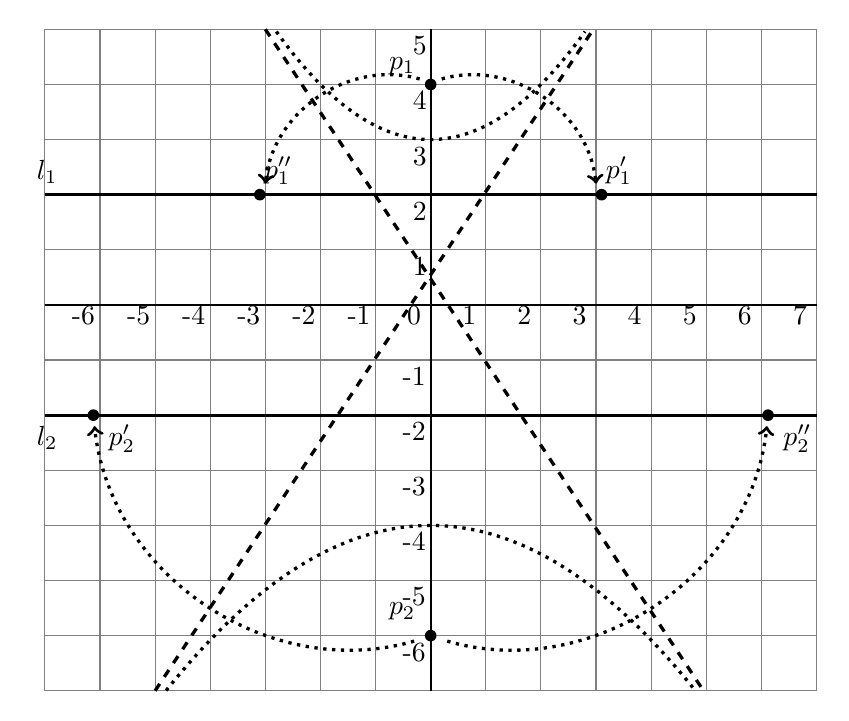
\begin{tikzpicture}[scale=.7]
\draw[step=10mm,white!50!black,thin] (-7,-7) grid (7,5);
\draw[thick] (-7,0) -- (7,0);
\draw[thick] (0,-7) -- (0,5);
\foreach \x in {-6,...,7}
  \node at (\x-.3,-.2) {\sm{\x}};
\foreach \y in {1,...,5}
  \node at (-.2,\y-.3) {\sm{\y}};
\foreach \y in {-6,...,-1}
  \node at (-.3,\y-.3) {\sm{\y}};
  
\coordinate (P1) at (0,4);
\fill (P1) circle (3pt) node[above left,xshift=-2pt] {$p_1$};
\coordinate (P2) at (0,-6);
\fill (P2) circle (3pt) node[above left,xshift=-2pt,yshift=2pt] {$p_2$};

\coordinate (P1P) at (3.1,2);
\fill (P1P) circle (3pt) node[above right,xshift=-2pt] {$p_1'$};
\coordinate (P2P) at (-6.12,-2);
\fill (P2P) circle (3pt) node[below right,xshift=2pt] {$p_2'$};

\coordinate (P1PP) at (-3.1,2);
\fill (P1PP) circle (3pt) node[above right,xshift=-2pt] {$p_1''$};
\coordinate (P2PP) at (6.12,-2);
\fill (P2PP) circle (3pt) node[below right,xshift=2pt] {$p_2''$};

\draw[very thick] (-7,2) -- node[very near start,above,xshift=-34pt] {$l_1$} (7,2);
\draw[very thick] (-7,-2) -- node[very near start,below,xshift=-34pt] {$l_2$} (7,-2);

\draw[domain=-4.8:4.8,samples=50,very thick,dotted] plot (\x,{-.13*\x*\x-4});
\draw[domain=-2.8:2.8,samples=50,very thick,dotted] plot (\x,{.25*\x*\x+3});

\draw[very thick,dashed] (-5,-7) -- (2.95,5);
\draw[very thick,dashed] (-3,5) -- (4.95,-7);

\draw[very thick,dotted,->,bend left=50] (.2,4.1) to (3,2.2);
\draw[very thick,dotted,->,bend left=50] (-.3,-6.1) to (-6.1,-2.2);

\draw[very thick,dotted,->,bend right=50] (-.2,4.1) to (-3,2.2);
\draw[very thick,dotted,->,bend right=50] (.3,-6.1) to (6.1,-2.2);
\end{tikzpicture}
\end{center}
\caption{אקסיומה 6}\label{f.axiom6}
\end{figure}

עבור נקודות נתונות וקווים נתונים יכולים להיות אפס, אחד, שניים או שלושה קיפולים.
איורים~
\ref{f.two-para-1}, \ref{f.two-para-2}
האיור בסעיף~
\ref{s.parabola}
מראה דוגמאות גרפיות לארבעת האפשרויות.

קיפול המניח את 
$p_i$
על
$l_i$
הוא קו שמרחקו ל-%
$p_i$
שווה למרחקו ל-%
$l_i$.
המקום הגיאומטרי של נקודות שהן במרחק שווה מנקודה
$p_i$
ומקו
$l_i$
הוא פרבולה עם מוקד 
\L{(focus)}
$p_i$
ומדריך
\L{(directrix)}
$l_i$.
קיפול הוא קו המשיק לפרבולה )סעיף~%
\ref{s.parabola}(.
כדי שהקיפול יניח בו-זמנית את 
$p_1$
על ל-%
$l_1$
ו-%
$p_2$
על ל-%
$l_2$,
הוא חייב להיות משיק משותף לשתי הפרבולות.

המשוואה עבור פרבולה שרירותית מסובכת ולכן נגביל את הדיון לפרבולה שציר ה-%
$y$
הוא ציר הסמטריה. נביא גם דוגמה עם פרבולה שציר הסמטריה שלה הוא ציר ה-%
$x$.


האיור~%
\ref{f.two-para-1}, 
\ref{f.two-para-2}
מראה את ארבעת האפשרויות של משיקים לפרבולה.

\begin{figure}[htb]
\begin{center}
\begin{subfigure}{.4\textwidth}
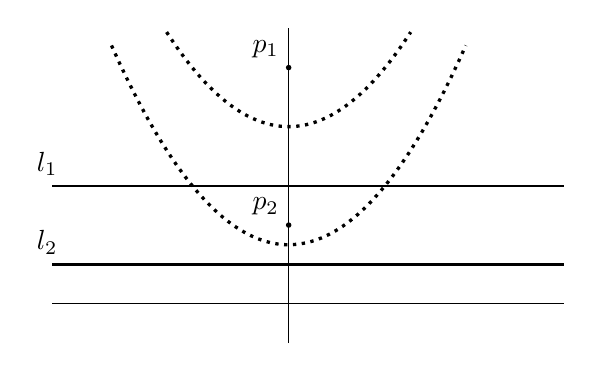
\begin{tikzpicture}[scale=.5]
\draw (-6,0) -- (7,0);
\draw (0,-1) -- (0,7);
\coordinate (P1) at (0,6);
\fill (P1) circle (2pt) node[above left] {$p_1$};
\coordinate (P2) at (0,2);
\fill (P2) circle (2pt) node[above left] {$p_2$};
\draw[thick] (-6,3) -- node[very near start,above,xshift=-25pt] {$l_1$} (7,3);
\draw[thick] (-6,1) -- node[very near start,above,xshift=-25pt] {$l_2$} (7,1);
\draw[domain=-3.1:3.1,samples=50,very thick,dotted] plot (\x,{.25*\x*\x+4.5});
\draw[domain=-4.5:4.5,samples=50,very thick,dotted] plot (\x,{.25*\x*\x+1.5});
\end{tikzpicture}
\caption{אפס משיקים}\label{f.two-para-0}
\end{subfigure}
\hspace{3em}
\begin{subfigure}{.4\textwidth}
\begin{tikzpicture}[scale=.5]
\draw (-6,0) -- (7,0);
\draw (0,-1) -- (0,7);
\coordinate (P1) at (-2,6);
\fill (P1) circle (2pt) node[above left] {$p_1$};
\coordinate (P2) at (3,2);
\fill (P2) circle (2pt) node[above left] {$p_2$};
\draw[thick] (-6,3) -- node[very near start,above,xshift=-25pt] {$l_1$} (7,3);
\draw[thick] (-6,1) -- node[very near start,above,xshift=-25pt] {$l_2$} (7,1);
\draw[domain=-5:1,samples=50,very thick,dotted] plot (\x,{.25*(\x+2)*(\x+2)+4.5});
\draw[domain=-1.8:7,samples=50,very thick,dotted] plot (\x,{.25*(\x-3)*(\x-3)+1.5});
\draw[very thick,dashed] (-5,5.85) -- (6,-.9);
\end{tikzpicture}
\caption{משיק אחד}\label{f.two-para-1}
\end{subfigure}
\end{center}
\end{figure}

\begin{figure}[htb]
\begin{center}
\begin{subfigure}{.4\textwidth}
\begin{tikzpicture}[scale=.5]
\draw (-7,0) -- (7,0);
\draw (0,-7) -- (0,5);
\coordinate (P1) at (0,4);
\fill (P1) circle (2pt) node[above left] {$p_1$};
\coordinate (P2) at (0,-6);
\fill (P2) circle (2pt) node[above left] {$p_2$};
\draw[thick] (-7,2) -- node[very near start,above,xshift=-25pt] {$l_1$} (7,2);
\draw[thick] (-7,-2) -- node[very near start,below,xshift=-25pt] {$l_2$} (7,-2);
\draw[domain=-4.8:4.8,samples=50,very thick,dotted] plot (\x,{-.13*\x*\x-4});
\draw[domain=-2.8:2.8,samples=50,very thick,dotted] plot (\x,{.25*\x*\x+3});
\draw[very thick,dashed] (-5,-7) -- (2.95,5);
\draw[very thick,dashed] (-3,5) -- (4.95,-7);
\end{tikzpicture}
\caption{}\label{}
\end{subfigure}
\hspace{3em}
\begin{subfigure}{.4\textwidth}
\begin{tikzpicture}[scale=.5]
\draw (-4,0) -- (7,0);
\draw (0,-4) -- (0,6);
\coordinate (P1) at (0,4);
\fill (P1) circle (2pt) node[above right] {$p_1$};
\coordinate (P2) at (4,0);
\fill (P2) circle (2pt) node[above right] {$p_2$};
\draw[thick] (-4,2) -- node[very near start,above,xshift=-25pt] {$l_1$} (7,2);
\draw[thick] (2,-4) -- node[very near start,left] {$l_2$} (2,7);
\draw[domain=-4:4,samples=50,very thick,dotted] plot (\x,{.25*\x*\x+3});
\draw[domain=3:7,samples=50,very thick,dotted] plot (\x,{sqrt(4*\x-12)});
\draw[domain=3:7,samples=50,very thick,dotted] plot (\x,{-sqrt(4*\x-12)});

\draw[thick,dashed,domain=-4:6.5] plot (\x,-\x+2);
\draw[thick,dashed,domain=-4:7] plot (\x,.27*\x+2.93);
\draw[thick,dashed,domain=2:4.8] plot (\x,3.73*\x-10.9);
\end{tikzpicture}
\caption{משיקים משותפים}\label{f.two-para-2}
\end{subfigure}
\end{center}
\end{figure}


\subsection{פיתוח הנקודה של הקיפול}

התיאור שלהלן מתייחס לאיור~%
\ref{f.parabola}.
הנקודה
$(0,f)$
היא מוקד של פרבולה עם מדריך
$y=d$.
נגדיר
$p=f-d$,
האורך 
)$\pm$(
של קטע הקו בין המוקד למדריך. אם הקודקוד 
\L{(vertex)}
נמצא על ציר ה-%
$x$,
המשוואה של הפרבולה היא
$y=\disfrac{x^2}{2p}$.
כדי להזיז את הפרבולה על ציר ה-%
$y$,
כך שהקודקוד שלה היא
$(0,h)$,
יש להוסיף 
$h$
למשוואת הפרבולה (איור%
~\ref{f.parabola}):
\[
y=\disfrac{x^2}{2p}+h\,.
\]
\begin{figure}[htb]
\begin{center}

\begin{tikzpicture}[scale=.8]
\draw (-6,0) -- node[very near start,below,xshift=-32pt] {$x$-axis}(6,0);
\draw (0,-3) -- node[very near start,right,yshift=-20pt] {$y$-axis}(0,4.5);
\draw[very thick] (-6,-2) -- node[near start,below] {directrix $\quad y=-2$} (6,-2);

%\draw (-6,0) -- node[very near start,below,xshift=-32pt] {$x$-\R{ציר}}(6,0);
%\draw (0,-3) -- node[very near start,right,yshift=-20pt] {$y$-\R{ציר}}(0,4.5);
%\draw[very thick] (-6,-2) -- node[near start,below] {\R{מדריך} $\quad y=-2$} (6,-2);

\draw[domain=-5:5,samples=50,very thick,dotted] plot (\x,{\x*\x/8+1});
\coordinate (F) at (0,4);
\fill (F) circle (2pt) node[left,xshift=-2pt,yshift=0pt] {$(0,f)=(0,4)$} node[above left,xshift=-2pt,yshift=4pt] {focus};
%\fill (F) circle (2pt) node[left,xshift=-2pt,yshift=0pt] {$(0,f)=(0,4)$} node[above left,xshift=-2pt,yshift=4pt] {\R{מוקד}};
\fill (0,-2) circle (2pt);
\fill (0,1) circle (2pt) node[below left] {vertex} node[below left,yshift=-10pt] {$(0,1)$};
%\fill (0,1) circle (2pt) node[below left] {\R{קודקוד}} node[below left,yshift=-10pt] {$(0,1)$};
\draw[<->] (2,-1.9) -- node[fill=white] {$p=6$} +(0,5.8);
\draw[<->] (1,.1) -- node[fill=white] {$h=1$} +(0,.8);
\end{tikzpicture}
\end{center}
\selectlanguage{hebrew}
\caption{הגדרת הפרבולה: מוקד, מדריך, קודקוד}\label{f.parabola}
\end{figure}
נגדיר
$a=2ph$
כך שמשוואת הפרבולה היא:
\begin{eqnlabels}
y&=&\disfrac{x^2}{2p}+\disfrac{a}{2p}\\
x^2-2py+a&=&0\,.
\end{eqnlabels}

עבור הפרבולה באיור~%
\ref{f.parabola}
המשוואה היא:

\begin{eqn}
x^2-2\cdot 6\,y + 2\cdot 6 \cdot 1&=&0\\
x^2-12y +12&=&0\,.
\end{eqn}
נציב את המשוואה של קו 
\textbf{שרירותי}
$y=mx+b$
במשוואה עבור הפרבולה ונקבל משוואה עבור נקודות החיתוך של הקו והפרבולה:

\begin{eqn}
x^2-2p(mx+b)+a&=&0\\
x^2+(-2mp)x+(-2pb+a)&=&0\,.
\end{eqn}
הקו יהיה משיק לפרבולה אם ורק אם למשוואה ריבועית זו קיים 
\textbf{בדיוק}
פתרון אחד אם ורק אם הדיסקרימננטה 
)\L{discriminant}(
היא אפס:
\begin{eqnlabels}
(-2mp)^2\:-\:4\cdot 1\cdot (-2pb+a)&=&0\\
m^2p^2+2pb-a&=&0\,.\label{eq.disc}
\end{eqnlabels}



משוואה זו עם המשתנה 
$m$ 
היא המשוואה ריבועית עבור השיפועים של המשיקים לפרבולה. קיימים אינסוף משיקים כי עבור כל 
$m$,
קיים
$b$
שגורם למשיק לזוז למעלה או למטה.%
\footnote{\R{פרט כמובן עבור קו המקביל לציר הסמטריה}.}
כדי למצוא את המשיקים המשותפים לשתי הפרבולות, יש לפתור את המשוואות של שתי הפרבולות, משוואות עם שני משתנים
$m$
ו-%
$b$.

%%%%%%%%%%%%%%%%%%%%%%%%%%%%%%%%%%%%%%%%%%%%%%%%%%%%%%%%%%%%%%%%

\begin{example}

\textbf{פרבולה 1:}
מוקד
$(0,4)$,
מדריך
$y=2$,
קודקוד
$(0,3)$.


$p=4-2=2$, $a=2\cdot 2\cdot 3=12$.
משוואת הפרבולה היא:
\[
x^2-2\cdot 2y +12=0\,.
\]
נציב לתוך משוואה%
~\ref{eq.disc}
ונפשט:
\[
m^2+b-3=0\,.
\]
\textbf{פרבולה 2:}
מוקד
$(0,-4)$,
מדריך
$y=-2$,
קודקוד
$(0,-3)$.

$p=-4-(-2)=-2$, $a=2\cdot -2\cdot -3=12$.
משוואת הפרבולה היא:
\[
x^2-2\cdot (-2)y+12=0\,.
\]
נציב לתוך משווארה%
~\ref{eq.disc}
ופשט:
\[
m^2-b-3=0\,.
\]
הפתרונות של שתי המשוואות:
\begin{eqn}
m^2+b-3&=&0\\
m^2-b-3&=&0\,,
\end{eqn}
הם
$m=\pm\sqrt{3}\approx \pm 1.73$
ו-%
$b=0$.
המשיקים המשותפים שהם הקיפולים הם:
\[
y=\sqrt{3}x\,,\quad y=-\sqrt{3}x\,.
\]
\end{example}

%%%%%%%%%%%%%%%%%%%%%%%%%%%%%%%%%%%%%%%%%%%%%%%%%%%%%%%%%%%%%%%%

\begin{example}

\textbf{פרבולה 1:}
ללא שינוי, המשוואה היא:
\[
m^2+b-3=0\,.
\]
\textbf{פרבולה 2:}
מוקד
$(0,-6)$,
מדריך
$y=-2$,
קודקוד
$(0,-4)$.

$p=-6-(-2)=-4$, $a=2\cdot -4\cdot -4=32$.
משוואת הפרבולה היא:
\[
x^2-2\cdot (-4)y +32=0\,.
\]
נציב לתוך משווארה%
~\ref{eq.disc}
ונפשט:
\[
2m^2-b-4=0\,.
\]
הפתרונות של שתי המשוואות:
\begin{eqn}
m^2+b-3&=&0\\
2m^2-b-4&=&0\,,
\end{eqn}
הם
$m=\pm\sqrt{\disfrac{7}{3}}\approx \pm 1.53$
ו-%
$b=\disfrac{2}{3}$.
יש שני משיקים משותפים שהם קיפולים:
\[
y=\sqrt{\disfrac{7}{3}}x+\disfrac{2}{3}\,,\quad y=-\sqrt{\disfrac{7}{3}}x+\disfrac{2}{3}\,.
\]
\end{example}

%%%%%%%%%%%%%%%%%%%%%%%%%%%%%%%%%%%%%%%%%%%%%%%%%%%%%%%%%%%%%%%%

\begin{example}

\textbf{פרבולה 1:}
ללא שינוי, המשוואה היא:
\[
m^2+b-3=0\,.
\]
\textbf{פרבולה 2:}
פרבולה שציר הסמטריה שלה הוא ציר ה-%
$x$.
מוקד
$(4,0)$,
מדריך
$x=2$,
קודקוד
$(3,0)$.
$p=4-2=2$, $a=2\cdot 2\cdot 3=12$.
משוואת הפרבולה היא:
\[
y^2-4x+12 = 0\,.
\]
שימו לב שזו משוואה עם 
$x$
ו-%
$y^2$
במקום
$x^2$
ו-%
$y$,
כך שלא ניתן להשתמש במשוואה%
~\ref{eq.disc}
ונצטרך לפתח את משוואות מחדש.

נציב את המשוואה של הקו:

\begin{eqn}
(mx+b)^2-4x+12&=&0\\
m^2x^2+(2mb-4)x+(b^2+12)&=&0\,
\end{eqn}
נשווה את הדיסקרימננטה לאפס ונפשט:

\begin{eqn}
(2mb-4)^2\:-\:4m^2(b^2+12)&=&0\\
-3m^2-mb+1&=&0\,.
\end{eqn}
אם ננסה לפתור את שתי המשוואות:

\begin{eqn}
m^2+b-3&=&0\\
-3m^2-mb+1&=&0\,,
\end{eqn}
נקבל משוואה 
\textbf{ממעלה שלוש}
במשתנה
$m$:
\begin{equation}
m^3-3m^2-3m+1=0\,.\label{eq.cubic}
\end{equation}
למשוואה ממעלה שלוש יש לפחות פתרון ממשי אחד ולכל היותר שלושה פתרונות ממשיים, לכן יכול להיות אחד, שניים או שלשה משיקים משותפים. הנוסחה למציאת פתרונות למשוואה ממעלה שלוש די מסובכת, לכן השתמשתי במחשבון באינטרנט וקיבלתי שלושה פתרונות:
\[
m=3.73\,, \;m=-1\,, \; m=0.27\,.
\]
אם נבחר
$m=0.27$, $b=3-m^2=2.93$,
משוואת הקיפול היא:
\[
y=0.27x+2.93\,.
\]
מהצורה של המשוואה%
~\ref{eq.cubic},
נוכל לנחש ש-%
$1$
או
$-1$
הוא פתרון:
\begin{eqn}
1^3-3\cdot 1^2-3\cdot 1+1&=&-4\\
(-1)^3-3\cdot (-1)^2-3\cdot(-1)+1&=&0\,.
\end{eqn}
נחלק את המשוואה%
~\ref{eq.cubic}
ב-%
$m-(-1)=m+1$
ונקבל משוואה ריבועית
$m^2-4m+1$
ששורשיה הם
$2\pm\sqrt{3}\approx 3.73, 0.27$.

\end{example}

%%%%%%%%%%%%%%%%%%%%%%%%%%%%%%%%%%%%%%%%%%%%%%%%%%%%%%%%%%%%%%%%

\subsection{פיתוח המשוואות של השיקופים}

נחשב את  
$p_1'=(x_1',y_1')$,
השיקוף של
$p_1=(x_1,y_1)$
מסביב למשיק
$l_t$
שהמשוואה שלה היא
$y=m_tx+b_t$.
)החישוב דומה עבור כל משיק ועבור
$p_2$.(
נמצא את הקו
$l_p$
עם המשוואה
$y=m_px+b_p$
שניצב ל-%
$l_t$
ועובר דרך
$p_1$:

\begin{eqn}
y&=&-\disfrac{1}{m_t}x+b_p\\
y_1&=&-\disfrac{1}{m_t}x_1+b_p\\
y&=&\disfrac{-x}{m_t}+\left(y_1+\disfrac{x_1}{m_t}\right)\,.
\end{eqn}
כעת נמצא את נקודת החיתוך 
$p_t=(x_t,y_t)$
של
$l_t$
ו-%
$l_p$:
\begin{eqn}
m_tx_t+b_t&=&\disfrac{-x_t}{m_t}+\left(y_1+\disfrac{x_1}{m_t}\right)\\
%x_t&=&\disfrac{\left(y_1+\disfrac{x_1}{m_t}-b_t\right)}{\left(m_t+\disfrac{1}{m_t}\right)}\\
x_t&=& \disfrac{m_t(y_1-b_t)+x_1}{m_t^2+1}\\
y_t&=&m_tx_t+b_t\,.
\end{eqn}
ניתן למצוא את השיקוף
$p_1'$
כי נקודת החיתוך
$p_t$
היא נקודת האמצע בין
$p_1$
לבין
$p_1'$:
\begin{eqn}
x_t&=&\disfrac{x_1+x_1'}{2}\,,\quad y_t=\disfrac{y_1+y_1'}{2}\\
x_1'&=&2x_t-x_1\,,\quad y_1'=2y_t-y_1\,.
\end{eqn}
\begin{example}
נתון
$p_1=(0,4)$
ו-%
$l_1$
עם המשוואה
$y=\sqrt{3}x$:
\begin{eqn}
%x_t&=&\disfrac{\left(4+\disfrac{0}{\sqrt{3}}-0\right)}{\left(\sqrt{3}+\disfrac{1}{\sqrt{3}}\right)}=\sqrt{3}\\
x_t&=&\disfrac{\sqrt{3}(4-0)+0}{(\sqrt{3})^2+1}=\sqrt{3}\\
y_t&=&\sqrt{3}\sqrt{3}+0=3\\
x_1'&=&2x_t-x_1=2\sqrt{3}-0=2\sqrt{3}\approx 3.46\\
y_1'&=&2y_t-y_1=2\cdot 3 - 4 = 2\,.
\end{eqn}
\end{example}

%%%%%%%%%%%%%%%%%%%%%%%%%%%%%%%%%%%%%%%%%%%%%%%%%%%%%%%

\subsection{משיקים לפרבולה}\label{s.parabola}

באיור~%
\ref{f.para:locus}
בחרנו חמש נקודות
$i=1,\ldots,5$, $p_i$
על הפרבולה. כל נקודה
$p_i$
היא במרחק
$a_i$
גם מהמוקד וגם מהמדריך. נוריד ניצב למדריך מ-%
$p_i$,
ונסמן ב-%
$p_i'$
את נקודת החיתוך של הניצב עם המדריך. נשתמש באקסיומה $2$ ונבנה את הקו 
$l_i$
דרך
$p_i$
שמשקף את 
$p$
על
$p_i'$.
האיור מראה את הקיפול 
$l_1$
דרך 
$p_1$.

\begin{figure}[htb]
\begin{center}

\begin{tikzpicture}[scale=.9]
\draw (-6,0) -- node[very near start,below,xshift=-32pt] {$x$-axis} (6,0);
\draw (0,-3) -- node[very near start,right,yshift=-20pt] {$y$-axis} (0,4.5);
\draw[ultra thick] (-6,-2) -- node[near end,below] {directrix $d: \quad y=-f$} (6,-2);
%\draw (-6,0) -- node[very near start,below,xshift=-32pt] {$x$-\R{ציר}} (6,0);
%\draw (0,-3) -- node[very near start,right,yshift=-20pt] {$y$-\R{ציר}} (0,4.5);
%\draw[ultra thick] (-6,-2) -- node[near end,below] {\R{מדריך} $d: \quad y=-f$} (6,-2);
\draw[domain=-6:6,samples=50,very thick,dotted] plot (\x,{\x*\x/8});
\coordinate (F) at (0,2);
\fill (F) circle (3pt) node[above left,xshift=-2pt,yshift=15pt] {$(0,f)$} node[above left,xshift=-2pt,yshift=30pt] {focus} node[above right] {$p$};
%\fill (F) circle (3pt) node[above left,xshift=-2pt,yshift=15pt] {$(0,f)$} node[above left,xshift=-2pt,yshift=30pt] {\R{מוקד}} node[above right] {$p$};
\fill (0,0) circle (1.5pt) node[below right] {$p_2$};
\fill (0,-2) circle (1.5pt);
\fill (2,-2) circle (1.5pt);
\fill (3,-2) circle (1.5pt);
\fill (5,-2) circle (1.5pt);
\coordinate (FP) at (-5,-2);
\fill (FP) circle (1.5pt) node[below] {$p_1'$};
\coordinate (F1) at (2,.5);
\fill (F1) circle (1.5pt) node[below right] {$p_3$};
\coordinate (F2) at (3,1.125);
\fill (F2) circle (1.5pt) node[below right] {$p_4$};
\coordinate (F3) at (5,3.125);
\fill (F3) circle (1.5pt) node[below right] {$p_5$};
\coordinate (F4) at (-5,3.125);
\fill (F4) circle (1.5pt) node[above right] {$p_1$};
\draw (F) -- node[left] {$a_2$} (0,0) -- node[left] {$a_2$} (0,-2);
\draw (F) -- node[near end,left] {$a_3$} (F1) -- node[left] {$a_3$} (2,-2);
\draw (F) -- node[near end,above] {$a_4$} (F2) -- node[left] {$a_4$} (3,-2);
\draw (F) -- node[above] {$a_5$} (F3) -- node[left] {$a_5$} (5,-2);
\draw (F) -- node[above] {$a_1$} (F4) -- node[left] {$a_1$} (FP);
\draw[very thick,dashed] ($(F4)!-.4!(-2.5,0)$) -- node[very near end,right,xshift=2pt] {$l_1$} ($(F4)!1.8!(-2.5,0)$);
\draw (0,-2) rectangle +(8pt,8pt);
\draw (2,-2) rectangle +(8pt,8pt);
\draw (3,-2) rectangle +(8pt,8pt);
\draw (5,-2) rectangle +(8pt,8pt);
\draw (-5,-2) rectangle +(8pt,8pt);
\end{tikzpicture}
\end{center}
\caption{המשיק כמקום הגיאומטרית}\label{f.para:locus}
\end{figure}

\begin{theorem}
הקיפולים הם משיקים לפרבולה.
\end{theorem}

\begin{proof}%
\footnote{אני מודה לאוריה בן-לולו שהראתה לי הוכחה זו.}
באיור~%
\ref{f.tangent-proof}
המוקד הוא 
$p$,
המדריך הוא 
$l$,
$p'$
היא נקודה על המדריך, ו-%
$m$
הוא הקיפול המשקף את
$p$
על 
$p'$.
לפי ההגדרה, 
$m$
הוא האנך האמצעי של הקו
$\overline{pp'}$.
תהי 
$s$
נקודת החיתוך של 
$\overline{pp'}$
ו-%
$m$.
אזי 
$\overline{ps}=\overline{p's}=a$
ו-%
$m\perp \overline{pp'}$.

\begin{figure}[htb]
\begin{center}

\begin{tikzpicture}[scale=.9]
\draw[ultra thick] (-6,-2) -- node[near end, below] {$l$} (6,-2);
\draw[domain=-5.5:5.5,samples=50,very thick,dotted] plot (\x,{\x*\x/8});
\coordinate (F) at (0,2);
\fill (F) circle (2pt) node[above right] {$p$};
\coordinate (FP) at (-3,-2);
\fill (FP) circle (1.5pt) node[below] {$p'$};
\coordinate (F4) at (-3,1.125);
\fill (F4) circle (1.5pt) node[above right] {$r$};
\coordinate (F5) at (-5,2.775);
\fill (F5) circle (1.5pt) node[left,yshift=-4pt] {$q$};
\coordinate (F5p) at (-5,-2);
\fill (F5p) circle (1.5pt) node[below] {$p''$};
\draw (F) -- node[above] {$b$} (F4) -- node[left] {$b$} (FP);
\draw (F) -- node[above] {$c$} (F5);
\draw (F5) -- node[left] {$d$} (F5p);
\draw[thick,dashed,name path=fold] ($(F4)+(140:4)$) -- (F4) -- node[below,xshift=-2pt,yshift=-2pt] {$m$} ($(F4)+(-40:5.1)$);
\draw (FP) rectangle +(8pt,8pt);
\draw (F5p) rectangle +(8pt,8pt);
\draw (F5) -- (FP);
\draw[name path=base] (F) -- (FP);
\path [name intersections = {of = base and fold, by = {G}}];
\fill (G) circle (1.5pt) node[below,yshift=-4pt] {$s$};
\draw[rotate=140] (G) rectangle +(6pt,6pt);
\path (FP) -- node[left] {$c$} (F5);
\path (F) -- node[below] {$a$} (G) -- node[below] {$a$} (FP);
\end{tikzpicture}
\end{center}
\caption{ההוכחה שקיפול הוא משיק}\label{f.tangent-proof}
\end{figure}
תהי
$r$
נקודת החיתוך של הניצב ל-%
$l$
דרך 
$p'$
והקיפול
$m$.
אזי
$\triangle psr\cong \triangle p'sr$
לפי צלע-זווית-צלע, כי
$\overline{ps}=\overline{p's}$, 
$\angle psr=\angle p'sr=90^\circ$
ו-%
$\overline{rs}$
הוא צלע משותפת. מכאן ש-%
$\overline{pr}=\overline{p'r}=b$
ולכן
$r$
נמצאת על הפרבולה.

בחרו נקודה
$p''$
על המדריך שהיא שונה מ-%
$p'$.
נניח שהקיפול
$m$
גם משקף את
$p$ 
על
$p''$.
תהי 
$q$
החיתוך של הניצב ל-%
$l$
דרך 
$p''$
והקיפול
$m$.
כמו בהוכחה לעיל, נוכל להוכיח ש-%
$\overline{pq}=\overline{p'q}=c$.
נסמן
$\overline{qp''}=d$.
אם
$q$
נמצאת על הפרבולה, אזי
$d=\overline{qp''}=\overline{qp}=c$.
אבל
$c$
הוא היתר של המשולש ישר-זווית
$\triangle qp''p'$
ולא ייתכן שהיתר שווה לאחת הצלעות של המשולש.
הוכחנו שלקיפול
$m$
נקודת חיתוך אחת עם בפרבולה, ולכן הקיפול הוא משיק.
\end{proof}

%%%%%%%%%%%%%%%%%%%%%%%%%%%%%%%%%%%%%%%%%%%%%%%%%%%%%%%%%%%%%%%%

\section{אקסיומה 7}\label{s.ax7}

\begin{axiom}
נתונה נקודה 
$p_1=(x_1,y_1)$,
ונתונים קווים
$l_1$,
$l_2$,
קיים קיפול
$l$
הניצב ל-%
$l_2$
שהמניח את
$p_1$
על ל-%
$l_1$
(איור~%
\ref{f.axiom7}).
\end{axiom}

\begin{figure}[htb]
\begin{center}

\begin{tikzpicture}[scale=.9]
\draw[step=10mm,white!50!black,thin] (-1,-1) grid (9,8);
\draw[thick] (-1,0) -- (9,0);
\draw[thick] (0,-1) -- (0,8);
\foreach \x in {0,...,9}
  \node at (\x-.2,-.2) {\sm{\x}};
\foreach \y in {1,...,8}
  \node at (-.2,\y-.3) {\sm{\y}};
  
\coordinate (P1) at (5,3);
\fill (P1) circle (2pt) node[below left] {$p_1$};

\coordinate (P1P) at (2.75,5.25);
\fill (P1P) circle (2pt) node[left,xshift=-4pt] {$p_1'$};

\draw[very thick] (1,0) -- node[very near start,right,xshift=2pt] {$l_1$} (3,6);
\draw[very thick,name path=l2] (8,3) -- node[very near start,right,xshift=-2pt,yshift=6pt] {$l_2$} (5,6);

\draw[thick,dotted] ($(1,0)!-.15!(3,6)$) -- ($(1,0)!1.34!(3,6)$);

\draw[thick,dotted] ($(8,3)!-.3!(5,6)$) -- ($(8,3)!1.65!(5,6)$);

\draw[thick,dotted] ($(P1)!-.4!(P1P)$) -- node[very near start,below,yshift=-4pt] {$l_p$} ($(P1)!1.5!(P1P)$);

\draw[very thick,dashed,name path=fold] (-.5,-.25) -- node[very near end,above,xshift=4pt,yshift=6pt] {$l$} (7.5,7.75);

\coordinate (mid) at ($(P1)!.5!(P1P)$);
\fill (mid) circle (2pt) node[below,yshift=-8pt] {$p_m$};

\path [name intersections = {of = fold and l2, by = {perp}}];
\draw[rotate=-45] (mid) rectangle +(8pt,8pt);
\draw[rotate=-45] (perp) rectangle +(8pt,8pt);


\draw[very thick,dotted,->,bend right=50] (5.1,3.2) to (3,5.2);
\end{tikzpicture}
\end{center}
\caption{אקסיומה 7}\label{f.axiom7}
\end{figure}

\textbf{פיתוח משוואת הקיפול:}
המשוואות של
$l_1$
ו-%
$l_2$
הן
$y = m_1x + b_1$ 
ו-% 
$y=m_2x+b_2$.
הקיפול
$l$
ניצב ל-%
$l_2$,
וגם ל-%
$l_p$
הניצב ל-%
$l$,
ולכן
$l_p\|l_2$.
$l_p$
עובר דרך
$p_1$.
נחשב:
\begin{eqn}
y&=&m_2x+b_p\\
y_1&=&m_2x_1+b_p\\
y&=&m_2x+(y_1-m_2x_1)\,.
\end{eqn}
$p_1'=(x_1',y_1')$,
השיקוף של
$p_1$
מסביב לקיפול
$l$,
היא נקודת החיתוך של 
$l_1$
ו-%
$l_p$:

\begin{eqn}
m_1x_1'+b_1&=&m_2x_1'+(y_1-m_2x_1)\\
x_1'&=&\disfrac{y_1-m_2x_1-b_1}{m_1-m_2}\\
y_1'&=&m_1x_i'+b_1\,.
\end{eqn}
$p_m=(x_m,y_m)$,
נקודת האמצע של
$l_p$,
נמצאת על הקיפול
$l$:
\[
(x_m,y_m)=\left(\disfrac{x_1+x_1'}{2},\disfrac{y_1+y_1'}{2}\right)\,.
\]
הקיפול
$l$
הוא האנך האמצעי של 
$\overline{p_1p_1'}$,
וכדי לחשב את המשוואה שלו, תחילה נחשב את
$p_m$,
נקודת האמצע של
$\overline{p_1p_1'}$:
\begin{eqn}
y_m&=&-\disfrac{1}{m_2}x_m+b_m\\
b_m&=&y_m+\disfrac{x_m}{m_2}\,.
\end{eqn}
המשוואה של הקיפול
$l$
היא:
\[
y=-\disfrac{1}{m_2}x+\left(y_m+\disfrac{x_m}{m_2}\right)\,.
\]
\begin{example}
נתונה הנקודה
$p_1=(5,3)$,
נתון הקו 
$l_1$
שהמשוואה שלו היא
$y=3x-3$,
ונתון הקו
$l_2$
שהמשוואה שלו היא
$y=-x+11$.

\begin{eqn}
x_1'&=&\disfrac{3-(-1)\cdot 5-(-3)}{3-(-1)}=\disfrac{11}{4}\\
y_1' &=&3\cdot\disfrac{11}{4} + (-3)=\disfrac{21}{4}\\
	p_m&=&\left(\disfrac{5+\disfrac{11}{4}}{2},\disfrac{3+\disfrac{21}{4}}{2}\right)=\left(\disfrac{31}{8},\disfrac{33}{8}\right)\,.
\end{eqn}
משוואת הקיפול היא:
\[
y=-\disfrac{1}{-1}\cdot x+\left(\disfrac{33}{8}+\disfrac{\disfrac{31}{8}}{-1}\right)=x+\disfrac{1}{4}\,.
\]
\end{example}

%%%%%%%%%%%%%%%%%%%%%%%%%%%%%%%%%%%%%%%%%%%%%%%%%%%

\subsection*{מה ההפתעה?}

אוריגמי, האומנות של קיפולי נייר, קיים מאות שנים, ולכן מפתיע שרק במאה העשרים פותחה הפורמליזציה שלו. מפתיע עוד יותר שקיים אקסיומתיזציה של קיפולי נייר. המתמטיקה של אורגמי היא דרך מצויינת ללמוד גיאומטריה אנליטית, תכונות של פרבולות והמושג מקום גיאומטרי.

\subsection*{מקורות}

ניתן למוצא את האקסיומות של אוריגמי ב-%
\cite{wiki:hh-axioms}.
\L{Lang}
\cite{lang}
מביא דוגמאות של יצירות אוריגמי.
\cite[Chap.~10]{martin}
מציג את התיאוריה המפורטת של אורגמי, כולל הוכחה שלפרבולה יכולה להיות אפס, אחד, שניים או שלושה משיקים. אוריה בן-לולו הראתה לי את ההוכחה של משפט%
~\ref{thm.parabola-tangents}.
מצאתי שתוכנה גיאומטרית כגון 
\L{Geogebra}
עוזרת להבין את הקשר בין הגיאומטריה והאלגברה של האקסיומות.

הצגה ברורה של משוואות קוביות ניתן למצוא בפרקים
$1,2$
של
\cite{jorg}.


\tikzsetfigurename{origami-cube}
% !TeX root = surprises.tex

\chapter{El método de Lill y el pliegue de Beloch}\label{c.origami-cube}

%%%%%%%%%%%%%%%%%%%%%%%%%%%%%%%%%%%%%%%%%%%%%%%%%%%%%%%%%%%%%%%

\section{Un truco de magia}\label{s.magic}
\index{Lill's method}

Construimos una trayectoria formada por cuatro segmentos $\{a_3=1,a_2=6,a_1=11,a_0=6\}$, partiendo del origen en la dirección positiva del eje $x$ y girando $90^\circ$ en sentido contrario a las agujas del reloj entre segmento y segmento. Construimos una segunda trayectoria de la siguiente manera: trazamos una recta desde el origen con un ángulo de $63,4^\circ$ y denotamos con $P$ su intersección con $a_2$. Giramos a la izquierda $90^\circ$, trazamos una recta y marcar su intersección con $a_1$ con $Q$. Giramos de nuevo $90^\circ$ a la izquierda, trazamos una recta y señalamos que interseca el final de la trayectoria en $(-10,0)$ (Fig.~\ref{f.magic}).

\begin{figure}[b]
\begin{center}
\begin{tikzpicture}[scale=.85]
% Draw help lines and axes
\draw[step=10mm,white!50!black] (-11,-1) grid (2,7);
\draw[thick] (-11,0) -- (2,0);
\draw[thick] (0,-1) -- (0,7);
\foreach \x in {-10,...,2}
  \node at (\x-.3,-.2) {\sm{\x}};
\foreach \y in {1,...,7}
  \node at (-.2,\y-.3) {\sm{\y}};

% Draw first path
\coordinate (A) at (0,0);
\coordinate (B) at (1,0);
\coordinate (C) at (1,6);
\coordinate (D) at (-10,6);
\coordinate (E) at (-10,0);
\draw[very thick] (A) --
  node[below,xshift=1pt,yshift=-10pt] {$a_3=1$} (B);
\draw[very thick,name path=bc] (B) -- 
  node[right,yshift=6pt] {$a_2=6$} (C);
\draw[very thick,name path=cd] (C) --
  node[above,xshift=4pt] {$a_1=11$}(D);
\draw[very thick,name path=de] (D) --
  node[left,xshift=3pt,yshift=6pt] {$a_0=6$}(E);

% Draw first segment of second path
\path[name path=a2] (A) -- +(63.4:4);
\path [name intersections = {of = a2 and bc, by = {A2}}];
\node[above right] at (A2) {$P$};
\draw[very thick,dashed] (A) -- (A2);
\draw ($(A) + (14pt,0)$)
  arc [start angle=0, end angle = 63.4, radius=14pt];
\node[above right,xshift=34pt,yshift=2pt] at (A) {$63.4^\circ$};
\draw[->] ($(A)+(32pt,8pt)$) -- +(-18pt,0);
\draw[rotate=153.4] (A2) rectangle +(7pt,7pt);

% Draw second segment of second path
\path[name path=b2] (A2) -- +(153.4:10);
\path [name intersections = {of = b2 and cd, by = {B2}}];
\node[above left] at (B2) {$Q$};
\draw[very thick,dashed] (A2) -- (B2);
\draw[rotate=243.4] (B2) rectangle +(7pt,7pt);

% Draw third segment of second path%
\draw[very thick,dashed] (B2) -- (E);
\end{tikzpicture}
\end{center}
\caption{Un truco de magia}\label{f.magic}
\end{figure}

Calcular el valor negativo de la tangente del ángulo al inicio del segundo del trayecto: $-\tan 63,4^\circ=-2$. Sustituimos este valor en el polinomio cuyos coeficientes son las longitudes de los segmentos del primer camino:
\begin{eqnarray*}
p(x)&=&a_3x^3+a_2x^2+a_1x+a_0\\
&=&x^3+6x^2+11x+6\\
p(-\tan 63.4^\circ)&=&(-2)^3+6(-2)^2+11(-2)+6=0\,.
\end{eqnarray*}
¡Hemos encontrado una raíz del polinomio cúbico $x^3+6x^2+11x+6$!

Continuemos con el ejemplo. El polinomio $p(x)=x^3+6x^2+11x+6$ tiene tres raíces $-1,-2,-3$. Calculamos el arcotangente de los valores negativos de las raíces  :
\[
\alpha=-\tan^{-1} (-1) = 45^\circ,\quad \beta=-\tan^{-1}(-2) \approx 63.4^\circ,\quad \gamma=-\tan^{-1}(-3)\approx 71.6^\circ\,.
\]
Para cada ángulo la segunda trayectoria interseca el final de la primera trayectoria (Fig.~\ref{f.cube-multiple}).

El valor $-\tan 56,3\approx -1,5$ no es una raíz de la ecuación. La figura~\ref{f.noroots} muestra el resultado de la aplicación del método para este ángulo. Esta trayectoria no se cruza con el segmento de línea para el coeficiente $a_0$ en $(-10,0)$.

\begin{figure}[b]
\begin{center}
\begin{tikzpicture}[scale=.85]
% Draw help lines and axes
\draw[step=10mm,white!50!black] (-11,-1) grid (2,7);
\draw[thick] (-11,0) -- (2,0);
\draw[thick] (0,-1) -- (0,7);
\foreach \x in {-10,...,2}
  \node at (\x-.3,-.2) {\sm{\x}};
\foreach \y in {1,...,7}
  \node at (-.2,\y-.3) {\sm{\y}};
\coordinate (A) at (0,0);
\coordinate (B) at (1,0);
\coordinate (C) at (1,6);
\coordinate (D) at (-10,6);
\coordinate (E) at (-10,0);
\draw[very thick] (A) --
  node[below,yshift=-5pt] {$1$} (B);
\draw[very thick,name path=bc] (B) -- 
  node[right,yshift=24pt] {$6$} (C);
\draw[very thick,name path=cd] (C) --
  node[above] {$11$}(D);
\path[name path=de] (D) -- ($(E)+(0,-.8)$);
\draw[very thick] (D) --
  node[left,yshift=6pt] {$6$} (E);

% Draw first segment of first second path
\path[name path=a1] (A) -- +(45:3);
\path [name intersections = {of = a1 and bc, by = {A1}}];
\node[above right] at (A1) {$P_1$};
\draw[very thick,dashed] (A) -- (A1);
\draw[thick] ($(A) + (16pt,0)$)
  arc [start angle=0, end angle = 45, radius=16pt];
\node[above right,xshift=44pt,yshift=0pt] at (A) {$\alpha$};
\draw[rotate=135] (A1) rectangle +(7pt,7pt);
\draw[Stealth-,thick] ($(A) + (15pt,5pt)$) -- +(24pt,0);

% Draw second segment of first second path
\path[name path=b1] (A1) -- +(135:8);
\path [name intersections = {of = b1 and cd, by = {B1}}];
\node[above right] at (B1) {$Q_1$};
\draw[very thick,dashed] (A1) -- (B1);
\draw[rotate=225] (B1) rectangle +(7pt,7pt);

% Draw third segment of first second path
\draw[very thick,dashed] (B1) -- (E);

% Draw first segment of second second path
\path[name path=a2] (A) -- +(63.4:4);
\path [name intersections = {of = a2 and bc, by = {A2}}];
\node[above right] at (A2) {$P_2$};
\draw[very thick,dashed] (A) -- (A2);
\draw[thick] ($(A) + (24pt,0)$)
  arc [start angle=0, end angle = 63.4, radius=24pt];
\node[above right,xshift=44pt,yshift=8pt] at (A) {$\beta$};
\draw[rotate=153.4] (A2) rectangle +(7pt,7pt);
\draw[<-,thick] ($(A) + (22pt,14pt)$) -- +(18pt,0);

% Draw second segment of second second path%
\path[name path=b2] (A2) -- +(153.4:10);
\path [name intersections = {of = b2 and cd, by = {B2}}];
\node[above right] at (B2) {$Q_2$};
\draw[very thick,dashed] (A2) -- (B2);
\draw[rotate=243.4] (B2) rectangle +(7pt,7pt);

% Draw third segment of second second path%
\draw[very thick,dashed] (B2) -- (E);

% Draw first segment of second second path%
\path[name path=a3] (A) -- +(71.6:4);
\path [name intersections = {of = a3 and bc, by = {A3}}];
\node[above right] at (A3) {$P_3$};
\draw[very thick,dashed] (A) -- (A3);
\draw[thick] ($(A) + (38pt,0)$)
  arc [start angle=0, end angle = 70, radius=40pt];
\node[above right,xshift=44pt,yshift=22pt] at (A) {$\gamma$};
\draw[rotate=161.6] (A3) rectangle +(7pt,7pt);
\draw[<-,thick] ($(A) + (32pt,25pt)$) -- +(10pt,0);

% Draw second segment of second second path%
\path[name path=b3] (A3) -- +(161.6:10);
\path [name intersections = {of = b3 and cd, by = {B3}}];
\node[above right] at (B3) {$Q_3$};
\draw[very thick,dashed] (A3) -- (B3);
\draw[rotate=251.6] (B3) rectangle +(7pt,7pt);

% Draw third segment of second second path%
\draw[very thick,dashed] (B3) -- (E);
\end{tikzpicture}
\end{center}
\caption{Método de Lill para las tres raíces del polinomio}\label{f.cube-multiple}
\end{figure}


\begin{figure}[t]
\begin{center}
\begin{tikzpicture}[scale=.85]
% Draw help lines and axes
\draw[step=10mm,white!50!black] (-11,-1) grid (2,7);
\draw[thick] (-11,0) -- (2,0);
\draw[thick] (0,-1) -- (0,7);
\foreach \x in {-10,...,2}
  \node at (\x-.3,-.2) {\sm{\x}};
\foreach \y in {1,...,7}
  \node at (-.2,\y-.3) {\sm{\y}};

% Draw first path
\coordinate (A) at (0,0);
\coordinate (B) at (1,0);
\coordinate (C) at (1,6);
\coordinate (D) at (-10,6);
\coordinate (E) at (-10,0);
\draw[very thick] (A) --
  node[below,yshift=-5pt] {$1$} (B);
\draw[very thick,name path=bc] (B) -- 
  node[right,yshift=6pt] {$6$} (C);
\draw[very thick,name path=cd] (C) --
  node[above] {$11$}(D);
\draw[very thick] (D) --
  node[left,yshift=6pt] {$6$}(E);
\path[name path=de] (-10,-1) -- (-10,7);

% Draw first segment of second path
\path[name path=a2] (A) -- +(56.3:3);
\path [name intersections = {of = a2 and bc, by = {A2}}];
\node[above right] at (A2) {$P$};
\draw[very thick,dashed] (A) -- (A2);
\draw ($(A) + (14pt,0)$)
  arc [start angle=0, end angle = 56.3, radius=14pt];
\node[above right,xshift=10pt,yshift=6pt] at (A) {$56.3^\circ$};
\draw[rotate=146.3] (A2) rectangle +(7pt,7pt);

% Draw second segment of second path
\path[name path=b2] (A2) -- +(146.3:10);
\path [name intersections = {of = b2 and cd, by = {B2}}];
\node[above right] at (B2) {$Q$};
\draw[very thick,dashed] (A2) -- (B2);
\draw[rotate=236.3] (B2) rectangle +(7pt,7pt);

% Draw third segment of second path
\path[name path=c2] (B2) -- +(236.3:8.5);
\path [name intersections = {of = c2 and de, by = {C2}}];
\vertex{C2};
\draw[very thick,dashed] (B2) -- (C2);
\end{tikzpicture}
\end{center}
\caption{Una trayectoria que no ilustra una raíz}\label{f.noroots}
\end{figure}

Este ejemplo muestra un método descubierto por Eduard Lill en 1867 para hallar gráficamente las raíces reales de cualquier polinomio. En realidad no estamos encontrando las raíces, sino verificando que un valor dado es una raíz.

La sección~\ref{s.method} presenta una especificación formal del método de Lill (limitado a polinomios cúbicos) y da ejemplos de cómo funciona en casos especiales. Una demostración de la corrección del método de Lill se da en la sección~\ref{s.proof}. La sección~\ref{s.beloch-fold} muestra cómo se puede implementar el método utilizando el axioma~6 de origami. Esto se llama el pliegue de Beloch y precedió a la formalización de los axiomas de origami durante muchos años.

\section{Especificación del método de Lill}\label{s.method}

\subsection{El método de Lill como algoritmo}
\index{Lill's method!algorithm}
\begin{itemize}
\item Comenzamos a partir de con un polinomio cúbico arbitrario $p(x)=a_3x^3+a_2x^2+a_1x+a_0$.
\item Construimos la primer trayectoria:
\begin{itemize}
\item Para cada coeficiente $a_3,a_2,a_1,a_0$ (en ese orden) construye un segmento de las respectivas longitudes, partiendo del origen $O=(0,0)$ en la dirección positiva del eje $x$. Giramos $90^\circ$ en sentido contrario a las agujas del reloj entre cada segmento.
\end{itemize}
\item Construimos el segundo camino:
\begin{itemize}
\item Construimos una recta desde $O$ formando un ángulo de $\theta$ con el eje $x$ positivo que intersecte a $a_2$ en el punto $P$.
\item Giramos $\pm 90^\circ$ y trazamos una recta desde $P$ que corte a $a_1$ en $Q$.
\item Giramos $\pm 90^\circ$ y construimos una recta desde $Q$ que intersecte a $a_0$ en $R$.
\item Si $R$ es el punto final de la primera trayectoria entonces $-\tan\theta$ es una raíz de $p(x)$.
\end{itemize}
\item Casos especiales:
\begin{itemize}
\item Al construir los segmentos de la primera trayectoria, si un coeficiente es negativo, construimos el segmento  \emph{hacia atrás}.
\item Al construir los segmentos de línea de la primera trayectoria, si un coeficiente es cero, no construimos un segmento, sino constinuamos con el siguiente giro de $\pm 90^\circ$.
\end{itemize}
\item Notes:
\begin{itemize}
\item La frase \emph{se cruza con $a_i$} significa \emph{interseca el segmento de línea $a_i$ o cualquier extensión de $a_i$}.
\item Al construir la segunda trayectoria, elegimos gira $90^\circ$ a la izquierda oa la derecha por $90^\circ$ para que haya una intersección con el siguiente segmento de la primera trayectoria o su extensión.
\end{itemize}
\end{itemize}

\begin{figure}[b]
\begin{center}
\begin{tikzpicture}[scale=.85]
% Draw help lines and axes
\draw[step=10mm,white!50!black] (-1,-5) grid (6,2);
\foreach \x in {0,...,6}
  \node at (\x-.3,-.2) {\sm{\x}};
\foreach \y in {-4,...,-1}
  \node at (-.3,\y-.3) {\sm{\y}};
\foreach \y in {1,...,2}
  \node at (-.3,\y-.3) {\sm{\y}};

% Draw first path
\coordinate (A) at (0,0);
\coordinate (B) at (1,0);
\coordinate (C) at (1,-3);
\coordinate (D) at (4,-3);
\coordinate (E) at (4,-4);
\draw[very thick,{Stealth[scale=1.4,inset=2pt,reversed]}-] (A) --
  node[below,yshift=-5pt] {$1$} (B);
\draw[very thick,{Stealth[scale=1.4,inset=2pt]}-,name path=bc] (B) -- 
  node[right,xshift=3pt] {$a_2=-3$} (C);
\draw[very thick,{Stealth[scale=1.4,inset=2pt]}-,name path=cd] (C) --
  node[above,xshift=11pt] {$a_1=-3$}(D);
\draw[very thick,{Stealth[scale=1.4,inset=2pt,reversed]}-,name path=de] (D) --
  node[right] {$1$}(E);

% Draw extensions of first path
\draw[very thick,loosely dotted,name path=a] (-1,0) -- (6,0);
\draw[very thick,loosely dotted,name path=b] (1,-5) -- (1,2);
\draw[very thick,loosely dotted,name path=c] (-1,-3) -- (6,-3);

% Draw first second path
\path[name path=a1] (A) -- +(-75:5);
\path [name intersections = {of = a1 and b, by = {B1}}];
\path[name path=b1] (B1) -- +(15:5);
\path [name intersections = {of = b1 and c, by = {C1}}];
\draw[thick,loosely dashed] (A) -- (B1) -- (C1) -- (E);

% Draw second second path
\draw[very thick,dashed] (4,-4) -- (5,-3) coordinate (A2);
\coordinate (P) at (5,-3);
\node[above right] at (P) {$Q$};
\draw[very thick,dashed] (5,-3) -- (1,1) coordinate (B2);
\coordinate (Q) at (1,1);
\node[above right] at (Q) {$P$};
\draw[very thick,dashed] (1,1) -- (0,0);

% Draw third second path
\path[name path=a3] (A) -- +(-15:5);
\path [name intersections = {of = a3 and b, by = {B3}}];
\path[name path=b3] (B3) -- +(-105:5);
\path [name intersections = {of = b3 and c, by = {C3}}];
\draw[thick,loosely dashed] (A) -- (B3) -- (C3) -- (E);
\end{tikzpicture}
\end{center}
\caption{Método de Lill con raíces negativas}\label{f.negative}
\end{figure}

\subsection{Coeficientes negativos}\label{s.negative}

Vamos a demostrar el método de Lill para el polinomio $p(x)=x^3-3x^2-3x+1$ con coeficientes negativos (Sec.~\ref{s.ax6}). Comenzamos construyendo un segmento de longitud $1$ a la derecha. A continuación, giramos $90^\circ$ hacia arriba, pero como el coeficiente es negativo, construimos un segmento de longitud $3$ hacia abajo, es decir, en dirección opuesta a la flecha. Tras girar $90^\circ$ hacia la izquierda, el coeficiente vuelve a ser negativo, así que construimos un segmento de longitud $3$ hacia la derecha. Por último, giramos hacia abajo y construimos un segmento de longitud $ 1 $ (Fig.~\ref{f.negative}, las líneas de trazos sueltos será discutido en Sec.~\ref{s.noninteger}).

\begin{figure}[b]
\begin{center}
\begin{tikzpicture}[scale=.7]
% Draw help lines and axes
\draw[step=10mm,white!50!black] (-1,-4) grid (11,7);
\foreach \x in {0,...,11}
  \node at (\x-.3,-.2) {\sm{\x}};
\foreach \y in {-3,...,-1}
  \node at (-.3,\y-.3) {\sm{\y}};
\foreach \y in {1,...,7}
  \node at (-.3,\y-.3) {\sm{\y}};

% Draw first path
\coordinate (A) at (0,0) node[above left] {$O$};
\coordinate (B) at (1,0);
\coordinate (C) at (8,0);
\coordinate (D) at (8,6);
\node[below right] at (D) {$A$};
\draw[very thick,{Stealth[scale=1.4,inset=2pt,reversed]}-] (A) --
  node[below,yshift=-5pt] {$1$} (B);
\draw[{Stealth[scale=1.4,inset=2pt,reversed]}-,very thick] (B) --
  ($(B)+(0,.1)$);
\draw[very thick,{Stealth[scale=1.4,inset=2pt]}-,name path=bc] (B) -- 
  node[below,xshift=-6pt,yshift=-5pt] {$-7$} (C);
\draw[very thick,{Stealth[scale=1.4,inset=2pt]}-,name path=cd] (C) --
  node[right,yshift=4pt] {$-6$}(D);

% Draw extensions of first path
\draw[very thick,loosely dotted] (1,-3) -- (1,7);
\draw[very thick,loosely dotted] (-1,0) -- (11,0);

% Draw first second path
\draw[very thick,dashed,->] (0,0) -- (1,-3);
\coordinate (P1) at (1,-3);
\node[below left] at (P1) {$P_1$};
\draw[very thick,dashed,->] (1,-3) coordinate (A1) -- (10,0);
\coordinate (Q1) at (10,0);
\node[below right] at (Q1) {$Q_1$};
\draw[very thick,dashed,->] (10,0) coordinate (B1) -- (D);

% Draw second second path
\draw[very thick,dashed,->] (0,0) -- (1,1) coordinate (A2);
\node[above right] at (A2) {$P_2$};
\draw[very thick,dashed,->] (A2) -- (2,0) coordinate (B2);
\node[below right] at (B2) {$Q_2$};
\draw[very thick,dashed,->] (B2) -- (D);

% Draw third second path
\draw[very thick,dashed,->] (0,0) -- (1,2) coordinate (A3);
\node[above left] at (A3) {$P_3$};
\draw[very thick,dashed,->] (A3) -- (5,0) coordinate (B3);
\node[below right] at (B3) {$Q_3$};
\draw[very thick,dashed,->] (B3) -- (D);
\end{tikzpicture}
\end{center}
\caption{Método de Lill con polinomios de coeficientes nulos}\label{f.zero}
\end{figure}

Comencemos el segundo camino con una línea a $ 45^\circ$ con el eje $x$ positivo. Se cruza con la extensión del segmento de línea para $a_2$ en $(1,1)$. Girando $-90^\circ$ (hacia la derecha), la recta interseca  interseca la prolongacion de $a_1$ en $(5,-3)$. Girando nuevamente $-90^\circ$, la recta interseca el final de la primera trayectoria en $(4,-4)$. Como $-\tan 45^\circ=-1$, hemos encontrado una raíz del polinomio:
\[p(-1)=(-1)^3-3(-1)^2-3(-1)+6=0\,.\]

Los segundos trayectos con los siguientes ángulos intersecan el final de la primera trayectoria:
\[
-\tan^{-1} (-1)= 45^\circ,\quad -\tan^{-1} (-2)\approx 63.4^\circ,\quad -\tan^{-1} 3\approx -71.6^\circ\,.
\]
Concluimos que hay tres raíces reales $\{-1,-2,3\}$.
Compruébalo:
\[
(x+1)(x+2)(x-3)=(x^2+3x+2)(x-3) =x^3-7x-6\,.
\]

\subsection{Coeficientes cero}\label{s.zero}
\index{Lill's method!zero coefficients}
$a_2$, el coeficiente del término $x^2$ del polinomio $x^3-7x-6=0$, es cero. Trazamos un segmento de longitud $0$, es decir, no trazamos una recta, pero sí giramos $\pm 90^\circ$ como indica la flecha que apunta hacia arriba en $(1,0)$ en la figura~\ref{f.zero}. Giramos nuevamente y trazamos un segmento de longitud $-7$, es decir, de longitud $7$ hacia atrás, hasta $(8,0)$. Por último, giramos una vez más y trazamos un segmento de longitud $-6 $ a $(8,6)$.

\begin{figure}[t]
\begin{center}
\begin{tikzpicture}[scale=1.3]
\clip (-1.1,-2.1) rectangle (4.2,2.2);
% Draw help lines and axes
\draw[step=10mm,white!70!black,] (-1,-2) grid (4,2);
\foreach \x in {0,...,4}
  \node at (\x-.2,-.1) {\sm{\x}};
\foreach \y in {-1}
  \node at (-.1,\y-.2) {\sm{\y}};
\foreach \y in {1,2}
  \node at (-.1,\y-.2) {\sm{\y}};

% Draw first path
\coordinate (A) at (0,0);
\node[above left] at (A) {$O$};
\coordinate (B) at (1,0);
\coordinate (C) at (3,0);
\coordinate (D) at (3,-1);
\node[below right] at (D) {$A$};
\draw[very thick] (A) -- node[above,yshift=2pt] {$1$} (B);
\draw[{Stealth[scale=1.4,inset=2pt,reversed]}-,very thick] ($(A)+(.1,0)$) --
  ($(A)+(.15,0)$);
\draw[{Stealth[scale=1.4,inset=2pt,reversed]}-,very thick] ($(B)+(0,.05)$) --
  ($(B)+(0,.1)$);
\draw[very thick,name path=bc] (B) -- 
  node[above,xshift=-4pt,yshift=2pt] {$-2$} (C);
\draw[{Stealth[scale=1.4,inset=2pt,reversed]}-,very thick] ($(B)+(.22,0)$) --
  ($(B)+(.17,0)$);
\draw[very thick,name path=cd] (C) --
  node[left] {$1$}(D);
\draw[{Stealth[scale=1.4,inset=2pt,reversed]}-,very thick] ($(C)+(0,-.05)$) --
 ($(C)+(0,-.1)$);

% Draw extensions of first path
\draw[very thick,loosely dotted,name path=b] (1,-2) -- (1,2);
\draw[very thick,loosely dotted,name path=c] (-1,0) -- (4,0);
\draw[very thick,loosely dotted,name path=d] (3,-2) -- (3,2);

% Draw first second path
\coordinate (A1) at (1,-1);
\draw[very thick,dashed,->] (0,0) -- (A1);
\node[below right] at (A1) {$P_1$};
\coordinate (B1) at (2,0);
\draw[very thick,dashed,->] (A1) -- (B1);
\node[above right,xshift=4pt] at (B1) {$Q_1$};
\draw[very thick,dashed,->] (B1) -- (D);
\draw[rotate=45] (A1) rectangle +(4pt,4pt);
\draw[rotate=-135] (B1) rectangle +(4pt,4pt);

% Draw second second path
\path[name path=a2] (0,0) -- +(-31.7:4);
\path [name intersections = {of = a2 and b, by = {A2}}];
\draw[very thick,dashed,->] (0,0) -- (A2);
\node[below left,xshift=-18pt] at (A2) {$P_2$};
\draw[<-] ($(A2)+(-2pt,-1pt)$) -- +(-165:15pt);
\path[name path=b2] (A2) -- +(58.3:2.5);
\path [name intersections = {of = b2 and c, by = {B2}}];
\draw[very thick,dashed,->] (A2) -- (B2);
\node[above] at (B2) {$Q_2$};
\draw[very thick,dashed,->] (B2) -- (D);
\draw[rotate=58.3]   (A2) rectangle +(4pt,4pt);
\draw[rotate=-121.7] (B2) rectangle +(4pt,4pt);

% Draw third second path
\path[name path=a3] (0,0) -- +(58.3:2.5);
\path [name intersections = {of = a3 and b, by = {A3}}];
\draw[very thick,dashed,->] (0,0) -- (A3);
\node[above left] at (A3) {$P_3$};
\path[name path=b3] (A3) -- +(-31.7:4);
\path [name intersections = {of = b3 and c, by = {B3}}];
\draw[very thick,dashed,->] (A3) -- (B3);
\node[above right] at (B3) {$Q_3$};
\path[name path=c3] (B3) -- +(-121.7:4);
\draw[very thick,dashed,->] (B3) -- (D);
\draw[rotate=-121.7]   (A3) rectangle +(4pt,4pt);
\draw[rotate=-211.7]   (B3) rectangle +(4pt,4pt);
\end{tikzpicture}
\end{center}
\caption{Método de Lill con raíces no enteras}\label{f.noninteger}
\end{figure}

\subsection{Raíces no enteras}\label{s.noninteger}
\index{Lill's method!non-integer roots}
La figura~\ref{f.noninteger} muestra el método de Lill para $p(x)=x^3-2x+1$. La primera trayectoria va de $(0,0)$ a $(1,0)$ y luego gira hacia arriba. El coeficiente de $x^2$ es cero por lo que no se construye ningún segmento y el trayecto gira a la izquierda. El siguiente segmento es de longitud $-2$ por lo que va hacia atrás desde $(1,0)$ hasta $(3,0)$. Finalmente, el trayecto gira hacia abajo y se construye un segmento de longitud $1$ desde $(3,0)$ hasta $(3,-1)$.


Es fácil ver que si la segunda trayectoria comienza en un ángulo de $ 45^\circ $ se cruzará con la primer trayectoria en $ (3,-1) $. Por lo tanto, $-\tan^{-1} (-45)^\circ=1$ es una raíz. Si dividimos $p(x)$ entre $x-1$, obtenemos el polinomio cuadrático $x^2+x-1$ cuyas raíces son:
\[
\frac{-1\pm\sqrt{5}}{2} \approx 0.62,\; -1.62\,.
\]
Hay dos segundas trayectorias adicionales: una que empieza en $-\tan^{-1} 0,62\approx -31,8^\circ$, y otra que empieza en $-\tan^{-1}(-1,62)\approx 58,3^\circ$.

El polinomio $p(x)=x^3-3x^2-3x+1$ (Sec.~\ref{s.negative}) tiene raíces $ 2\pm\sqrt{3}\approx 3,73, 0,27$. Los ángulos correspondientes son $-\tan^{-1} 3,73 \approx -75^\circ$ y $-\tan^{-1} 0,27 \approx -15^\circ$ como muestran las líneas discontinuas de la figura~\ref{f.negative}.

\subsection{La raíz cúbica de dos}\label{s.cube}
\index{Lill's method!cube root of two}
Para duplicar un cubo, calculamos $\sqrt[3]{2}$, una raíz del polinomio cúbico $x^3-2$. En la construcción de la primera trayectoria, giramos dos veces a la izquierda sin construir ningún segmento, porque $a_2$ y $a_1$ son ambos cero. Luego se vuelve a girar a la izquierda (para mirar hacia abajo) y se construye hacia atrás (hacia arriba) porque $a_0=-2$ es negativo. El primer segmento de la segunda trayectoria se construye con un ángulo de $-\tan^{-1} \sqrt[3]{2}\approx -51.6^\circ$ (Fig.~\ref{f.cube-two}).

\begin{figure}[t]
\begin{center}
\begin{tikzpicture}[scale=1]
% Draw help lines and axes
\draw[step=10mm,white!70!black,] (-1,-2) grid (3,3);
\foreach \x in {0,...,3}
  \node at (\x-.2,-.1) {\sm{\x}};
\foreach \y in {-1}
  \node at (-.2,\y-.2) {\sm{\y}};
\foreach \y in {1,2,3}
  \node at (-.2,\y-.2) {\sm{\y}};

% Draw first path
\coordinate (A) at (0,0);
\coordinate (B) at (1,0);
\coordinate (C) at (1,2);
\draw[very thick] (A) -- node[above,yshift=2pt] {$1$} (B);

\draw[{Stealth[scale=1.4,inset=2pt,reversed]}-,very thick] ($(A)+(.05,0)$) --
  ($(A)+(.1,0)$);
\draw[{Stealth[scale=1.4,inset=2pt,reversed]}-,very thick] ($(B)+(0,.05)$) --
  ($(B)+(0,.1)$);
\draw[{Stealth[scale=1.4,inset=2pt,reversed]}-,very thick] ($(B)+(.1,.3)$) --
  ($(B)+(.08,.3)$);
\draw[{Stealth[scale=1.4,inset=2pt,reversed]}-,very thick] ($(B)+(0,.55)$) --
  ($(B)+(0,.5)$);

\draw[very thick] (B) -- 
  node[left,yshift=6pt] {$-2$} (C);

% Draw extensions of first path
\draw[very thick,loosely dotted,name path=a] (-1,0) -- (3,0);
\draw[very thick,loosely dotted,name path=b] (1,-2) -- (1,3);

% Draw first segment of second path
\path[name path=a1] (0,0) -- +(-51.6:2);
\path [name intersections = {of = a1 and b, by = {A1}}];
\draw[very thick,dashed,->] (A) -- (A1);
\node[below left] at (A1) {$P_1$};
\draw[rotate=38.4]   (A1) rectangle +(8pt,8pt);

% Draw second segment of second path
\path[name path=b1] (A1) -- +(38.4:2.5);
\path [name intersections = {of = b1 and a, by = {B1}}];
\draw[very thick,dashed,->] (A1) -- (B1);
\node[above right] at (B1) {$Q_1$};
\draw[rotate=128.4] (B1) rectangle +(8pt,8pt);

% Draw third segement of second path
\draw[very thick,dashed,->] (B1) -- (C);
\end{tikzpicture}
\end{center}
\caption{La raíz cúbica de dos}\label{f.cube-two}
\end{figure}


\begin{figure}[t]
\begin{center}
\begin{tikzpicture}[scale=.8]
% Draw grid and axes
\draw[step=10mm,white!50!black] (-11,-1) grid (2,7);
\draw[thick] (-11,0) -- (2,0);
\draw[thick] (0,-1) -- (0,7);
\foreach \x in {-10,...,2}
  \node at (\x-.3,-.2) {\sm{\x}};
\foreach \y in {1,...,7}
  \node at (-.2,\y-.3) {\sm{\y}};
  
% Draw the points of the first path
\coordinate (A) at (0,0);
\coordinate (B) at (1,0);
\coordinate (C) at (1,6);
\coordinate (D) at (-10,6);
\coordinate (E) at (-10,0);
\draw[rotate=90] (B) rectangle +(7pt,7pt);
  
% Draw A -- B and arrow
\draw[very thick] (A) --(B);
\draw[thick,<->] ($(A)+(0,-16pt)$) --
  node[fill=white] {$1$} ($(B)+(0,-16pt)$);

% Draw B -- C and arrow
\draw[very thick,name path=bc] (B) -- (C);
\draw[thick,<->] ($(B)+(42pt,0)$) --
  node[fill=white] {$a_2$} ($(C)+(44pt,0)$);

% Draw C -- D and arrow
\draw[very thick,name path=cd] (C) --(D);
\draw[thick,<->] ($(C)+(0,24pt)$) -- 
  node[fill=white] {$a_1$} ($(D)+(0,24pt)$);

% Draw D -- E and arrow
\draw[very thick,name path=de] (D) -- (E);
\draw[thick,<->] ($(D)+(-16pt,0)$) --
  node[fill=white] {$a_0$} ($(E)+(-16pt,0)$);

% Draw first angled segment of the second path and intersection A2 with BC
\path[name path=a2] (A) -- +(63.4:4);
\path [name intersections = {of = a2 and bc, by = {A2}}];
\node[above right] at (A2) {$P$};
\draw[very thick,dashed] (A) -- (A2);
\path (B) -- node[right] {$b_2$} (A2);
\path (A2) -- node[right,xshift=-1pt,yshift=8pt] {$a_2\!-\!b_2$} (C);
\draw[rotate=153.4] (A2) rectangle +(7pt,7pt);

% Draw second segment of the second path and intersection B2 with CD
\path[name path=b2] (A2) -- +(153.4:10);
\path [name intersections = {of = b2 and cd, by = {B2}}];
\node[above right] at (B2) {$Q$};
\draw[very thick,dashed] (A2) -- (B2);
\draw[rotate=243.4] (B2) rectangle +(7pt,7pt);
\path (D) -- node[above] {$a_1\!-\!b_1$} (B2); 
\path (B2) -- node[above] {$b_1$} (C);

% Draw third segment of the second path to E
\draw[very thick,dashed] (B2)-- (E);

% Label A, A2, B2 with theta
\draw ($(A) + (14pt,0)$)
  arc [start angle=0, end angle = 63.4, radius=14pt];
\node[above right,xshift=10pt,yshift=8pt] at (A) {$\theta$};
\draw ($(A2) + (0,14pt)$)
  arc [start angle=90, end angle = 153.4, radius=14pt];
\node[above left,xshift=-4pt,yshift=14pt] at (A2) {$\theta$};
\draw ($(B2) + (-14pt,0)$)
  arc [start angle=180, end angle = 243.4, radius=14pt];
\node[below left,xshift=-14pt,yshift=-4pt] at (B2) {$\theta$};
\end{tikzpicture}
\end{center}
\caption{Prueba del método de Lill}\label{f.lill-proof}
\end{figure}

\section{Prueba del método de Lill}\label{s.proof}
\index{Lill's method!proof of}

La demostración es para polinomios cúbicos mónicos $p(x)=x^3+a_2x^2+a_1x+a_0$. Si el polinomio no es mónico, se divide por $a_3$ y el polinomio resultante tiene las mismas raíces. En la figura~\ref{f.lill-proof} los segmentos de la primera trayectoria están denotados con los coeficientes y con $b_2,b_1,a_2-b_2,a_1-b_1$. En un triángulo rectángulo si un ángulo agudo es $\theta$ el otro ángulo es $90^\circ-\theta$. Por tanto, el ángulo sobre $P$ y el ángulo a la izquierda de $Q$ son iguales a $\theta$. He aquí las fórmulas de $\tan \theta$ calculadas a partir de los tres triángulos:
\begin{eqnarray*}
\tan \theta &=& \frac{b_2}{1}=b_2\\
\tan \theta &=& \frac{b_1}{a_2-b_2}=\frac{b_1}{a_2-\tan\theta}\\
\tan \theta &=& \frac{a_0}{a_1-b_1}=\frac{a_0}{a_1-\tan\theta(a_2-\tan\theta)}\,.
\end{eqnarray*}
Simplificamos la última ecuación, multiplicamos por $-1$ e incluimos $-1$ en las potencias:
\begin{eqnarray*}
(\tan\theta)^3-a_2(\tan\theta)^2+a_1(\tan\theta)-a_0&=&0\\
(-\tan\theta)^3+a_2(-\tan\theta)^2+a_1(-\tan\theta)+a_0&=&0\,.
\end{eqnarray*}
Se deduce que $-\tan\theta$ es una raíz real de $p(x)=x^3+a_2x^2+a_1x+a_0$.

\begin{figure}[t]
\begin{center}
\begin{tikzpicture}[scale=.6]
% Draw help lines and axes
\draw[step=10mm,white!60!black] (-11,-1) grid (3,13);
\draw[thick] (-11,0) -- (3,0);
\draw[thick] (0,-1) -- (0,13);
\foreach \x in {-10,...,3}
  \node at (\x-.3,-.2) {\sm{\x}};
\foreach \y in {1,...,13}
  \node at (-.2,\y-.3) {\sm{\y}};
  
% Draw first path with five points
\coordinate (A) at (0,0);
\coordinate (B) at (1,0);
\coordinate (C) at (1,6);
\coordinate (D) at (-10,6);
\coordinate (E) at (-10,0);
\node[below right,yshift=-6pt] at (A) {$P$};
\node[below left,yshift=-6pt] at (E) {$Q$};

\draw[thick] (A) -- (B);
\draw[thick,name path=bc] (B) -- node[right,near end] {$a_2$} (C);
\draw[thick,name path=cd] (C) -- node[above] {$a_1$} (D);
\draw[thick,name path=de] (D) -- (E);

% Draw parallel lines
\draw[thick,name path=bpcp] ($(B)+(1,-1)$) --
  node[above right] {$a_2'$}
  ($(C)+(1,7)$);
\draw[thick,name path=cpdp] ($(C)+(2,6)$) -- 
  node[above left,xshift=-24pt] {$a_1'$} 
  ($(D)+(-1,6)$);

% Draw first segment of second path
\path[name path=a2] (A) -- +(63.4:4);
\path [name intersections = {of = a2 and bc, by = {A2}}];
\draw[ultra thick,dotted] (A) -- (A2);
\node[above right,xshift=4pt] at (A2) {$R$};
\draw[rotate=153.4] (A2) rectangle +(10pt,10pt);

% Draw second segment of second path
\path[name path=b2] (A2) -- +(153.4:10);
\path [name intersections = {of = b2 and cd, by = {B2}}];
\node[above left] at (B2) {$S$};
\draw[very thick,dashed] (A2) -- (B2);
\draw[rotate=243.4] (B2) rectangle +(10pt,10pt);

% Draw third segment of second path
\draw[ultra thick,dotted] (B2) -- (E);

% Locate reflections on parallel lines and draw lines
\coordinate (PP) at ($(A2)+(1,2)$);
\node[above right] at (PP) {$P'$};
\draw[ultra thick,dotted] (A2) -- (PP);

\coordinate (QP) at ($(B2)+(3,6)$);
\node[above right] at (QP) {$Q'$};
\draw[ultra thick,dotted] (B2) -- (QP);
\end{tikzpicture}
\end{center}
\caption{El pliegue de Beloch para encontrar una raíz de $x^3+6x^2+11x+6$}\label{f.beloch-fold2}
\end{figure}

\begin{figure}[t]
\begin{center}
\begin{tikzpicture}[scale=.8]
% Draw help lines and axes
\draw[step=10mm,white!50!black] (-1,-5) grid (6,2);
\foreach \x in {0,...,6}
  \node at (\x-.3,-.2) {\sm{\x}};
\foreach \y in {-4,...,-1}
  \node at (-.3,\y-.3) {\sm{\y}};
\foreach \y in {1,...,2}
  \node at (-.3,\y-.3) {\sm{\y}};

% Draw first path
\coordinate (A) at (0,0);
\coordinate (B) at (1,0);
\coordinate (C) at (1,-3);
\coordinate (D) at (4,-3);
\coordinate (E) at (4,-4);
\node[above left] at (A) {$P$};
\node[below right] at (E) {$Q$};
\draw[very thick,{Stealth[scale=1.4,inset=2pt,reversed]}-] (A) --
  (B);
\draw[very thick,{Stealth[scale=1.4,inset=2pt]}-,name path=bc] (B) -- 
  node[left] {$a_2$} (C);
\draw[very thick,{Stealth[scale=1.4,inset=2pt]}-,name path=cd] (C) --
  node[above] {$a_1$}(D);
\draw[very thick,{Stealth[scale=1.4,inset=2pt,reversed]}-,name path=de] (D) --
 (E);

% Draw extensions of first path
\draw[very thick,loosely dotted,name path=b] (1,-4) -- (1,2);
\draw[very thick,loosely dotted,name path=c] (-1,-3) -- (6,-3);

% Draw reflected points
\coordinate (PP) at (2,2);
\coordinate (QP) at (6,-2);
\node[above left] at (PP) {$P'$};
\node[below right] at (QP) {$Q'$};

% Midpoints of bisected lines
\coordinate (R) at (1,1);
\coordinate (S) at (5,-3);
\node[above left] at (R) {$R$};
\node[below right] at (S) {$S$};

% Draw reflected lines
\draw[thick] ($(B)+(1,2)$) --
  node[right,very near end,yshift=-8pt] {$a_2'$} ($(C)+(1,-2)$);
\draw[thick] ($(C)+(-2,1)$) --
  node[above,very near start,xshift=-8pt,yshift=-1pt] {$a_1'$} ($(D)+(2,1)$);
\draw[ultra thick,dotted] (A) -- (PP);
\draw[ultra thick,dotted] (E) -- (QP);

% Draw fold
\draw[very thick,dashed] (R) -- (S);
\draw[rotate=-45] (R) rectangle +(8pt,8pt);
\draw[rotate=45] (S) rectangle +(8pt,8pt);
\end{tikzpicture}
\end{center}
\caption{El pliegue de Beloch para encontrar una raíz de $x^3-3x^2-3x+1$}\label{f.beloch-fold3}
\end{figure}

\section{El pliegue de Beloch}\label{s.beloch-fold}

Margharita P. Beloch descubrió una notable conexión entre el plegado y el método de Lill: una aplicación de la operación más tarde conocida como el sexto axioma del origami genera una raíz real de un polinomio cúbico. La operación se denomina a menudo \emph{pliegue de belloch}.


Consideremos el polinomio $p(x)=x^3+6x^2+11x+6$ (Sec.~\ref{s.magic}). Recordemos que un pliegue es la mediatriz del segmento entre un punto cualquiera y su reflexión alrededor del pliegue. Queremos que $\overline{RS}$ en la figura~\ref{f.beloch-fold2} sea la mediatriz de $\overline{QQ'}$ y $\overline{PP'}$, donde $Q',P'$ son las reflexiones de $Q,P$ alrededor de $\overline{RS}$, respectivamente.

Construimos una recta $a_2'$ paralela a $a_2$ a la misma distancia de $a_2$ que $a_2$ de $P$, y construimos una recta $a_1'$ paralela a $a_1$ a la misma distancia de $a_1$ que $a_1$ de $Q$. Aplicamos el axioma~6 para situar simultáneamente $P$ en $P'$ sobre $a_2'$ y para situar $Q$ en $Q'$ sobre $a_1'$. El pliegue $\overline{RS}$ es la mediatriz de las rectas $\overline{PP'}$ y $\overline{QQ'}$ por lo que los ángulos en $R$ y $S$ son ambos rectos como lo exige el método de Lill.

La figura ~\ref{f.beloch-fold3} muestra el pliegue de Beloch para el polinomio $x^3-3x^2-3x+1$ (Sec.~\ref{s.negative}). $a_2$ es el segmento vertical de longitud $3$ cuya ecuación es $x=1$, y su recta paralela es $a_2'$ cuya ecuación es $x=2$, porque $P$ está a una distancia de $1$ de $a_2$. $a_1$ es el segmento horizontal de longitud $3$ cuya ecuación es $y=-3$, y su recta paralela es $a_1'$ cuya ecuación es $y=-2$ porque $Q$ está a una distancia de $1$ de $a_1$. El pliegue $\overline{RS}$ es la mediatriz tanto de $\overline{PP'}$ como de $\overline{QQ'}$, y la recta $\overline{PRSQ}$ es la misma que la segunda trayectoria de la figura~\ref{f.negative}.

\newpage

\subsection*{¿Cuál es la sorpresa?}

Ejecutar el método de Lill como un truco de magia nunca deja de sorprender. Puede realizarse durante una presentación utilizando un programa de gráficos como GeoGebra. También sorprende que el método de Lill, publicado en $1867$, y el pliegue de Beloch, publicado en $1936$, precedieran en muchos años a la axiomatización del origami.

\subsection*{Fuentes}

Este capítulo se basa en \cite{bradford, hull-beloch, riaz}.


\tikzsetfigurename{origami-constructions}
% !TeX root = surprises.tex

%%%%%%%%%%%%%%%%%%%%%%%%%%%%%%%%%%%%%%%%%%%%%%%%%%%%%%%%%%%%%%%%

\chapter{בניות גיאומטריות באוריגמי}\label{c.origami-constructions}

בפרק זה נראה שבניות עם אוריגמי חזקים יותר מבניות עם סרגל ומחוגה. נביא שתי בניות לחלוקת זווית לשלושה חלקים, הראשונה של 
\L{Hisashi Abe}
(סעיף%
~\ref{s.abe-trisection})
והשנייה של
\L{George E. Martin}
(סעיף%
~\ref{s.martin-trisection}),
שתי בניות להכפלת קוביה, הראשונה של
\L{Peter Messer}
(סעיף%
~\ref{s.messer})
והשנייה של
\L{Marghareta P. Beloch}
(סעיף%
~\ref{s.cube2}).
הבנייה האחרונה היא של מתושע
\L{nonagon},
מצולע משוכלל עם תשעה צלעות (סעיף%
~\ref{s.nonagon}).

\section{הבנייה של 
\L{\normalsize Abe}\label{s.abe-trisection}
לחלוקת זווית לשלושה חלקים%
}\label{s.trisection-abe}

נתונה זווית חדה
$\angle PQR$,
נבנה את הקו
$p$
ניצב ל-%
$\overline{QR}$
ב-%
$Q$
והקו
$q$
ניצב ל-%
$p$
ב-% 
$A$
כך שהוא חותך את
$\overline{PQ}$.
נבנה את הקו
$r$,
האנך האמצעי של
$\overline{AQ}$
שחותך אותו בנקודה
$B$.
לפי אקסיומה 
$6$
נבנה קיפול
$l$
המניח את 
$A$
על
$\overline{PQ}$ 
בנקודה
$A'$
ומניח את
$Q$
על
$r$
בנקודה
$Q'$.
תהי
$B'$
השיקוף של 
$B$
מסביב ל-%
$l$.
נבנה את הקווים
$\overline{QB'}$
ו-%
$\overline{QQ'}$
(איור%
~\ref{f.abe1}).

\begin{figure}[tb]
\begin{center}
\begin{tikzpicture}[scale=.8]
% Place points P, Q, R
\coordinate (P) at (60:10cm); %(5,8.67);
\coordinate (Q) at (0,0);
\coordinate (R) at (10,0);
\fill (P) circle (2pt) node[below right] {$P$};
\fill (Q) circle (2pt) node[left] {$Q$};
\fill (R) circle (2pt) node[right] {$R$};

% Draw PQR
\draw [very thick] (P)  -- (Q) -- (R);

% Draw perpendicular to QR
\draw [thick] (Q) -- node[left,very near end] {$p$} +(0,11);

% Draw parallel to QR and parallel halfway
\coordinate (A) at (0,5);
\coordinate (B) at (0,2.5);
\draw [thick] (A) -- node[above,very near end] {$q$} +(10,0);
\draw [thick] (B) -- node[above,very near end] {$r$} +(10,0);
\fill (A) circle (2pt) node[left] {$A$};
\fill (B) circle (2pt) node[left] {$B$};
\path (Q) -- node[left] {$a$} (B) -- node[left] {$a$} (A);
\draw (A) rectangle +(8pt,8pt);
\draw (B) rectangle +(8pt,8pt);

% Tangent line y = -2.75x + 10.69

% Draw fold
\coordinate (D) at (0,10.69);
\coordinate (fold-x) at (3.89,0);
\coordinate (AP) at (3.65,6.33);
\coordinate (QP) at (6.87,2.5);
\coordinate (BP) at (5.26,4.42);
\fill (D) circle (2pt) node[left] {$D$};
\fill (AP) circle (2pt) node[above,yshift=6pt] {$A'$};
\fill (QP) circle (2pt) node[above,yshift=6pt] {$Q'$};
\fill (BP) circle (2pt) node[above,xshift=2pt,yshift=2pt] {$B'$};
\draw [very thick,dashed] (D) -- node[left,near start] {$l$} (fold-x);

% Draw line of reflections
\draw [very thick, dotted] (D) -- (QP);

% Draw trisecting lines
\draw [very thick,dotted] (Q) -- ($(Q)!1.3!(QP)$);
\draw [very thick,dotted] (Q) -- ($(Q)!1.3!(BP)$);

% Complete triangle
\draw [very thick,dotted] (A) -- (QP);

% Draw fold arrows
\draw[thick,dotted,->,bend left=40]
  ($(A)+(4pt,10pt)$) to ($(AP)+(-4pt,0pt)$);
\draw[thick,dotted,->,bend right=40]
  ($(Q)+(2pt,-4pt)$) to ($(QP)+(0pt,-4pt)$);

\end{tikzpicture}
\selectlanguage{hebrew}
\caption{הבנייה של
\L{Abe}
לחלוקת זווית לשלושה חלקים}
\label{f.abe1}
\end{center}
\end{figure}

\begin{theorem}
$\angle PQB'=\angle B'QQ'=\angle Q'QR=\angle PQR/3$.
\end{theorem}
\begin{proof}(1)
הנקודות
$A', B', Q'$
הן שיקופים סביב אותו קו 
$l$
של הנקודות
$A,B,Q$
הנמצאות על קו אחד
$\overline{DQ}$,
ולכן הן נמצאות על קטע קו אחד
$\overline{DQ'}$.
לפי הבנייה,
$\overline{AB}=\overline{BQ}$,
$\angle ABQ'=\angle QBQ'=90^\circ$,
$\overline{BQ'}$
הוא צלע משותף, כך ש-%
$\triangle ABQ'\cong \triangle QBQ'$ 
לפי צלע-זווית-צלע. מכאן ש-%
$\angle AQA'=\angle QAQ'=\alpha$
ו-%
$\triangle AQ'Q$
הוא שווה-שוקיים (איור~
\ref{f.first-proof}).

\begin{figure}[tb]
\begin{center}
\begin{tikzpicture}[scale=.8]

% Place points P, Q, R
\coordinate (P) at (60:10cm);
\coordinate (Q) at (0,0);
\coordinate (R) at (10,0);
\node[below right] at (P) {$P$};
\node[left,xshift=-4pt] at (Q) {$Q$};
\node[right] at (R) {$R$};

% Draw PQR
\draw (Q) -- (R);

% Draw perpendicular to QR
\draw (Q) -- node[left,very near end] {$p$} +(0,11);

% Draw parallel to QR and parallel halfway
\coordinate (A) at (0,5);
\coordinate (B) at (0,2.5);
\draw (A) -- node[above,very near end] {$q$} +(10,0);
\draw[name path=Br] (B) -- node[above,very near end] {$r$} +(10,0);
\node[left,xshift=-4pt] at (A) {$A$};
\node[left,xshift=-4pt] at (B) {$B$};
\path (Q) -- node[left,xshift=-4pt] {$a$} (B) -- node[left,xshift=-4pt] {$a$} (A);
\draw (A) rectangle +(8pt,8pt);
\draw (B) rectangle +(8pt,8pt);
\draw (Q) rectangle +(8pt,8pt);

% Tangent line y = -2.75x + 10.69

% Draw fold
\coordinate (D) at (0,10.69);
\coordinate (fold-x) at (3.89,0);
\coordinate (AP) at (3.65,6.33);
\coordinate (QP) at (6.87,2.5);
\coordinate (BP) at (5.26,4.42);
\node[left] at (D) {$D$};
\node[above,yshift=6pt] at (AP)  {$A'$};
\node[above,xshift=2pt,yshift=6pt] at (QP) {$Q'$};
\node[right,xshift=4pt,yshift=2pt] at (BP) {$B'$};
\draw[name path=fold,very thick,dashed] (D) -- node[left,near start] {$l$}  ($(D)!1.03!(fold-x)$);
	
% Draw line of reflections
\draw (D) -- (AP);

% Draw trisecting lines
\draw (Q) -- ($(Q)!1.3!(BP)$);

\draw [very thick,loosely dash dot,red] (Q) -- (QP);
\draw [very thick,loosely dash dot,red] (QP) -- (AP);
\draw [very thick,loosely dash dot,red] (AP) -- (Q);
\draw [very thick,loosely dash dot dot,blue] ($(Q)+(0,-4pt)$) -- ($(QP)+(0,-4pt)$);
\draw [very thick,dash dot dot,blue] ($(QP)+(0,-4pt)$) -- ($(A)+(0,-4pt)$);
\draw [very thick,dash dot dot,blue] ($(A)+(-4pt,0)$) -- ($(Q)+(-4pt,0)$);

\draw (A) -- (AP);

\node[left,xshift=-40pt,yshift=7pt] at (QP) {$\alpha$};
\node[left,xshift=-40pt,yshift=-6pt] at (QP) {$\alpha$};
\node[right,xshift=40pt,yshift=6pt] at (Q) {$\alpha$};
\node[right,xshift=40pt,yshift=28pt] at (Q) {$\alpha$};
\node[right,xshift=30pt,yshift=42pt] at (Q) {$\alpha$};

\draw (AP) -- (P);

\path[name path=Qr] (Q) -- (QP);
\path[name intersections = {of = fold and Qr, by = {U}}];
\node[above left,xshift=-2pt,yshift=-2pt] at (U) {$U$};
\draw[rotate=20] (U) rectangle +(8pt,8pt);
\path[name intersections = {of = fold and Br, by = {V}}];
\node[above left,xshift=-2pt,yshift=-2pt] at (V)  {$V$};
\end{tikzpicture}
\end{center}
\selectlanguage{hebrew}
\caption{%
הוכחות של הבנייה של
\L{Abe}
(נשתמש ב-%
$U,V$
בהוכחה השנייה)}
\label{f.first-proof}
\end{figure}
בגלל השיקוף
$\triangle AQ'Q\cong \triangle A'QQ'$,
ולכן גם
$\triangle A'QQ'$
הוא משולש שווה-שוקיים.
$\overline{QB'}$,
השיקוף של 
$\overline{Q'B}$,
הוא האנך האמצעי של משולש שווה-שוקיים ולכן
$\angle A'QB'=\angle Q'QB'=\alpha$.
לפי זוויות מתחלפות
$\angle Q'QR=\angle QQ'B=\alpha$.
ביחד:
\[
\triangle PQB'=\angle A'QB'=\angle B'QQ'=\angle Q'QR=\alpha\,.
\]
\end{proof}

\begin{proof}(2)
הקו
$l$
הוא קיפול ולכן הוא האנך האמצעי של
$\overline{QQ'}$.
נסמן ב-%
$U$
את נקודת החיתוך של
$l$
עם
$\overline{QQ'}$,
נסמן ב-%
$V$
את נקודת החיתוך שלו עם
$\overline{QB'}$
(איור%
~\ref{f.first-proof}).
$\triangle VUQ\cong \triangle VUQ'$
לפי צלע-זווית-צלע כי
$\overline{VU}$
הוא צלע משותף, הזוויות ב-%
$U$
הן זוויות ישרות, ו-%
$\overline{QU}=\overline{Q'U}$.
מכאן ש-%
$\angle VQU=\angle VQ'U=\alpha$
ו-%
$\angle Q'QR=\angle VQ'U=\alpha$
לפי זוויות מתחלפות.

כמו בהוכחה הראשונה, 
$A', B', Q'$
הן כולן שיקופים סביב
$l$,
ולכן הן כולן נמצאות על קטע קו אחד
$\overline{DQ'}$,
ו-%
$\overline{A'B'}=\overline{AB}=\overline{BQ}=\overline{B'Q'}=a$.
מכאן ש-%
$\triangle A'B'Q\cong\triangle Q'B'Q$
לפי צלע-זווית-צלע ו-%
$\angle A'QB'=\angle Q'QB'=\alpha$.
\end{proof}

\section{הבנייה של
\L{\normalsize Martin}
לחלוקת זווית לשלושה חלקים%
}\label{s.martin-trisection}
\begin{figure}[tb]
\begin{center}

\begin{tikzpicture}[scale=.9]

% Place points P, Q, R
\coordinate (P) at (60:10cm); %(5,8.67);
\coordinate (Q) at (0,0);
\coordinate (R) at (10,0);
\fill (P) circle (2pt) node[below right] {$P$};
\fill (Q) circle (2pt) node[above left] {$Q$};
\fill (R) circle (2pt) node[right] {$R$};

% Draw PQR
\draw (R)  -- (Q);
\draw [name path=pq] (Q) -- (P);

% M is the midpoint of PQ
\coordinate (M) at (2.5, 4.33);
\fill (M) circle (2pt) node[above left,xshift=2pt] {$M$};
\draw [rotate=-90] (M) rectangle +(8pt,8pt);

% Drop a perpendicular from M to QR and extend the line upwards
% This is the given line p
\coordinate (pQR) at (M |- Q);
\draw [thick,name path=p] (pQR) --
   node[left, very near end,yshift=28pt] {$p$}
   ($(pQR)!2!(M)$);
\draw (pQR) rectangle +(8pt,8pt);

% Construct q perpendicular to p through M
\draw [thick,name path=q] ($(M)+(-2,0)$) --
   node[above, very near start,xshift=-30pt] {$q$}
   ($(M)+(10,0)$);

% Construct the fold line t
% Its equation is y = -2.75x + 18.51, as obtained from Geogebra
\coordinate (t1) at (6.7,.085);
\coordinate (t2) at (3.5,8.89);
\draw [very thick,dashed,name path=t] (t1) --
   node[very near end,left] {$l$}
   (t2);

% Construct a perpendicular to t through P
\coordinate (perp-p) at ($(t1)!(P)!(t2)$);
\path [name path=perp-p] (P) -- ($(P)!2.5!(perp-p)$);

% Get its intersection with t denoted Pt
% and its intersection with p named PP
\path [name intersections = {of = t and perp-p, by = {Pt}}];
\path [name intersections = {of = p and perp-p, by = {PP}}];
\fill (PP) circle(2pt) node[left] {$P'$};
\draw [rotate=22] (Pt) rectangle +(8pt,8pt);

% Draw PT
\draw (P) -- (PP);

% Construct a perpendicular to t through Q
\coordinate (perp-q) at ($(t1)!(Q)!(t2)$);
\path[name path=perp-q] (Q) -- ($(Q)!2.1!(perp-q)$);

% Get its intersection with t denoted V
% and its intersection with q denoted S=Q'
\path [name intersections = {of = t and perp-q, by = {V}}];
\path [name intersections = {of = q and perp-q, by = {QP}}];
\fill (QP) circle(2pt) node[above,yshift=4pt] {$Q'$};
\fill (V) circle(2pt) node[above left,xshift=-4pt,yshift=-2pt] {$V$};
\draw [rotate=22] (V) rectangle +(8pt,8pt);

% Draw Q QP
\draw [name path=qs] (Q) -- (QP);

% Get the intersection of QS with p denoted U
\path [name intersections = {of = p and qs, by = {U}}];
\fill (U) circle(2pt) node[above left] {$U$};

% Draw PP QP
\draw [name path=ts] (PP) -- (QP);

% Get its intersection with QP denoted W
\path [name intersections = {of = ts and pq, by = {W}}];
\fill (W) circle(2pt) node[right,xshift=4pt,yshift=4pt] {$W$};

% Label line segments
\path (P) -- node[left] {$a$} (M);
\path (M) -- node[left]  {$a$} (Q);
\path (PP) -- node[left]  {$b$} (M);
\path (M) -- node[right] {$b$} (U);
\path (Q) -- node[below,near end] {$c$} (V);
\path (V) -- node[below] {$c$} (QP);

% Label angles
\node [xshift=5pt,yshift=20pt]        at (M) {$\gamma$};
\node [xshift=-5pt,yshift=-20pt]      at (M) {$\gamma$};
\node [xshift=18pt,yshift=15pt]       at (Q) {$\beta$};
\node [xshift=-18pt,yshift=-15pt]     at (P) {$\beta$};
\node [left,xshift=-30pt,yshift=7pt]  at (QP) {$\alpha$};
\node [left,xshift=-30pt,yshift=-7pt] at (QP) {$\alpha$};
\node [right,xshift=34pt,yshift=7pt]  at (Q) {$\alpha$};
\end{tikzpicture}
\end{center}
\selectlanguage{hebrew}
\caption{בנייה של Martin}\label{f.martin}
\end{figure}

\textbf{בנייה}
נתונה זווית חדה
$\angle PQR$
תהי
$M$
נקודת האמצע של
$\overline{PQ}$.
בנו
$p$
ניצב ל-%
$\overline{QR}$
העובר דרך
$M$
ובנו
$q$
ניצב ל-%
$p$
העובר דרך 
$M$.
$q$
מקביל ל-%
$\overline{QR}$.
לפי אקסיומה $6$ בנו קיפול
$l$
המניח את
$P$
ב-%
$P'$
על
$p$,
ומניח את
$Q$
ב-%
$Q'$
על
$q$.
ייתכן שקיים מספר קיפולים מתאימים; בחרו את הקיפול החותך את
$\overline{PM}$.
בנו את קטעי הקו
$\overline{PP'}$
ו-%
$\overline{QQ'}$
(איור~%
\ref{f.martin}).

\begin{theorem}
$\angle Q'QR = \angle PQR/3$.
\end{theorem}

\begin{proof}
סמנו ב-%
$U$
את נקודת החיתוך של
$\overline{QQ'}$
עם
$p$,
וסמנו ב-%
$V$
את נקודת החיתוך שלו עם
$l$.
סמנו ב-%
$W$
את החיתוכים של 
$\overline{PQ}$
ו-%
$\overline{P'Q'}$
עם
$l$.
לא ברור מאליו ש-%
$\overline{PQ}$
ו-%
$\overline{P'Q'}$
חותכים את
$l$
באותה נקודה. אבל
$\triangle PWP'\sim\triangle QQQ'$
כך שהגבהים מחלקים את שתי הזוויות הקודקודיות
$\angle PWP', \angle QWQ'$
והם חייבים להיות על אותו קו.

$\triangle QMU\cong \triangle PMP'$
לפי זווית-צלע-זווית:
$\angle P'PM=\angle UQM=\beta$
לפי זוויות מתחלפות,
$\overline{QM}=\overline{MP}=a$
כי 
$M$
היא נקודת האמצע של
$\overline{PQ}$
ו-%
$\angle QMU=\angle PMP'=\gamma$
כי הן זוויות קודקודיות. מכאן ש-%
$\overline{P'M}=\overline{MU}=b$.

$\triangle P'MQ'\cong\triangle UMQ'$
לפי צלע-זוויות-צלע: הראנו ש-%
$\overline{P'M}=\overline{MU}=b$,
הזוויות ב-%
$M$
הן זוויות ישרות,
$\overline{MQ'}$
הוא צלע משותף. הגובה של המשולש שווה-שוקיים 
$\triangle P'Q'U$ 
הוא חוצה הזווית
$\angle P'Q'U$
ולכן
$\angle P'Q'M=\angle UQ'M=\alpha$.
בנוסף,
$\angle UQ'M=\angle Q'QR=\alpha$
לפי זוויות מתחלפות.

$\triangle QWV\cong\triangle Q'WV$
לפי צלע-זווית-צלע:
$\overline{QV}=\overline{VQ'}=c$
הזוויות ב-%
$V$
ישרות ו-%
$\overline{VW}$
הוא צלע משותף. מכאן ש:
\begin{eqn}
\angle WQV&=&\beta=\angle WQ'V=2\alpha\\
\angle PQR &=& \beta + \alpha = 3\alpha\,.
\end{eqn}
\end{proof}

%%%%%%%%%%%%%%%%%%%%%%%%%%%%%%%%%%%%%%%%%%%%%%%%%%%%%%%%%%%%%%%

\newpage

\section{הבנייה של 
\L{\normalsize Messer}
להכפלת קוביה}%
\label{s.messer}

לקוביה בנפח 
$V$
צלעות באורך
$\sqrt[3]{V}$.
לקוביה עם נפח פי שניים אורכי הצלעות הם
$\sqrt[3]{2 V}=\sqrt[3]{2} \sqrt[3]{V}$,
ולכן אם נוכל לבנות קטע קו באורך
$\sqrt[3]{2}$,
נוכל להכפיל באורך הנתון
$\sqrt[3]{V}$
כדי להכפיל את הקוביה.

\textbf{בנייה:}
נקח דף נייר שהוא ריבוע ונקפל אותו לחצי כדי למצוא את הנקודת
$I=(0,1/2)$,
$Q=(1,1/2)$
(איור~%
\ref{f.lang}).
נבנה את קטעי הקו
$\overline{AC}$
ו-%
$\overline{BJ}$.
אפשר לחשב את הקואורדינטות של נקודה החיתוך 
$K=(2/3,1/3)$
על ידי פתרון המשוואות 
$y=1-x$
ו-%
$y=x/2$.

\begin{figure}[tb]
\begin{center}
\begin{tikzpicture}[scale=.55]
% Draw square
\coordinate (A) at (0,12);
\coordinate (B) at (0,0);
\coordinate (C) at (12,0);
\coordinate (D) at (12,12);

\node[left]  at (A) {$A=(0,1)$};
\node[left]  at (B) {$B=(0,0)$};
\node[right] at (C) {$C=(1,0)$};
\node[right] at (D) {$D=(1,1)$};

\draw [thick] (A)  -- (B) -- (C) -- (D) -- cycle;

% Divide a side in half

\coordinate (M)  at (0,6);
\coordinate (N) at (12,6);
\node[left] at (M) {$I=(0,1/2)$};
\node[right] at (N) {$J=(1,1/2)$};
\draw [thick,dashed] (M) -- (N);


\draw [very thick,dotted,name path=ac] (A) -- 
   node[near start,above,xshift=24pt] {$y=1-x$} (C);
\draw [very thick,dotted,name path=be2] (B) -- 
   node[near start,above,xshift=-12pt] {$y=x/2$} (N);

\path [name intersections = {of = ac and be2, by = {I}}];
\node[below,xshift=-6pt,yshift=-8pt] at (I) {$K=$};
\node[below,xshift=-6pt,yshift=-20pt] at (I) {$(2/3,1/3)$};

\coordinate (E)  at (0,4);
\coordinate (F) at (12,4);
\node[left] at (E) {$E=(0,1/3)$};
\node[right] at (F) {$F=(1,1/3)$};
\draw [thick,dashed] (E) -- (F);

\coordinate (G)  at (0,8);
\coordinate (H) at (12,8);
\node[left] at (G) {$G=(0,2/3)$};
\node[right] at (H) {$H=(1,2/3)$};
\draw (G) -- (H);
\end{tikzpicture}
\end{center}
\selectlanguage{hebrew}
\caption{בניית קטע קו באורך
 $1/3$}\label{f.lang}
\end{figure}
נבנה את הקו
$\overline{EF}$
ניצב ל-%
$\overline{AB}$
דרך 
$K$,
ונבנה את 
$\overline{GH}$,
השיקוף של
$\overline{BC}$
סביב
$\overline{EF}$.
חילקנו את צלע הריבוע לקטעים באורך 
$1/3$.

נשמתש באקסיומה $6$ כדי להניח את 
$C$
ב-%
$C'$
על
$\overline{AB}$,
ולהניח את
$F$
ב-%
$F'$
על
$\overline{GH}$.
נסמן ב-%
$L$
את נקודת החיתוך של הקיפול עם
$\overline{BC}$ 
ונסמן 
ב-%
$b$
את אורכו של
$\overline{BL}$.
נשנה את סימון הצלע של הריבוע ל-%
$a+1$
כאשר
$a=\overline{AC'}$.
אורכו של
$\overline{LC}$
הוא
$(a+1)-b$
(איור~%
\ref{f.doubling}).
\begin{theorem}
$\overline{AC'}=\sqrt[3]{2}$.
\end{theorem}

\begin{proof}
לאחר ביצוע הקיפול, קטע הקו
$\overline{LC'}$
הוא שיקוף של קטע הקו
$\overline{LC}$
מאותו אורך, וקטע הקו
$\overline{C'F'}$
הוא שיקוף של קטע הקו
$\overline{CF}$.
מכאן ש:
\begin{equation}
\overline{GC'}=a-\disfrac{a+1}{3}=\disfrac{2a-1}{3}\,.\label{eq.one-third}
\end{equation}
$\angle FCL$
היא זווית ישרה, לכן גם
$\angle F'C'L$ 
היא זווית ישרה.
\begin{figure}[tb]
\begin{center}
\begin{tikzpicture}[scale=.65]
% Draw and label square
\coordinate (A) at (0,12);
\coordinate (B) at (0,0);
\coordinate (C) at (12,0);
\coordinate (D) at (12,12);
\node[left]  at (A) {$A$};
\node[left]  at (B) {$B$};
\node[right] at (C) {$C$};
\node[right] at (D) {$D$};
\draw (B) rectangle +(9pt,9pt);
\draw[rotate=90] (C) rectangle +(9pt,9pt);
\draw [thick] (A)  -- (B) -- (C) -- (D) -- cycle;

% Draw line one-third from botton
\coordinate (E)  at (0,4);
\coordinate (F) at (12,4);
\node[left] at (E) {$E$};
\node[right] at (F) {$F$};
\draw [name path=ef] (E) -- (F);

% Draw line two-thirds from bottom
\coordinate (G)  at (0,8);
\coordinate (H) at (12,8);
\node[left] at (G) {$G$};
\node[right] at (H) {$H$};
\draw[rotate=-90] (G) rectangle +(9pt,9pt);
\draw (G) -- (H);

% Draw reflections of C and F
\coordinate (CP) at (0,5.31);
\coordinate (FP) at (2.96,8);
\node[left] at (CP) {$C'$};
\node[above right,yshift=8pt] at (CP) {$\alpha$};
\node[below right,xshift=-2pt,yshift=-12pt] at (CP) {$\alpha'$};
\node[above] at (FP) {$F'$};
\node[below left,xshift=-8pt] at (FP) {$\alpha'$};
\draw[rotate=-50] (CP) rectangle +(9pt,9pt);
\draw (CP) -- (FP);

% Draw fold and fold arrows
% Tangent is y = 2.26x - 10.9
% Crosses x axis at (4.83,0)
\coordinate (J) at (4.83,0);
\node[below] at (J) {$L$};
\node[above left,xshift=-8pt] at (J) {$\alpha$};
\draw [very thick,dashed,name path=jd] (J) -- node[very near end,left] {$l$} (10,12);
\draw[thick,dotted,bend right=40,->] (C) to ($(CP)+(4pt,0)$);
\draw[thick,dotted,bend right=40,->] (F) to ($(FP)+(4pt,4pt)$);

% Draw hypotenuses of right triangles
\draw (CP) -- (J);
\path (J)  -- (C);

% Labels on BC and hypotenuses
\path (CP) -- node[right] {$(a+1)-b$} (J);
\path (J)  -- node[below] {$(a+1)-b$} (C);
\path (B)  -- node[below] {$b$} (J);
\path (C)  -- node[right] {$\displaystyle\frac{a+1}{3}$} (F);
\path (CP) -- node[right,xshift=10pt] {$\displaystyle\frac{a+1}{3}$} (FP);

% Labels on AB
\draw[<->] ($(A)+(-1,0)$)    --
  node[fill=white] {$a$} ($(CP)+(-1,0)$);
\draw[<->] ($(CP)+(-1,0)$)   --
  node[fill=white] {$1$} ($(B)+(-1,0)$);
\draw[<->] ($(CP)+(-2.5,0)$) --
  node[fill=white] {$\displaystyle\frac{2a-1}{3}$} ($(G)+(-2.5,0)$);
\draw[<->] ($(A)+(-2.5,0)$) --
  node[fill=white] {$\displaystyle\frac{a+1}{3}$} ($(G)+(-2.5,0)$);
\end{tikzpicture}
\end{center}
\selectlanguage{hebrew}
\caption{בניית
$\sqrt[3]{2}$}
\label{f.doubling}
\end{figure}

$\triangle C'BL$
הוא משולש ישר-זווית ולפי משפט פיתגורס:
\begin{eqnlabels}
1^2 + b^2 &=& ((a+1)-b)^2\\
b&=&\disfrac{a^2+2a}{2(a+1)}\label{eq.value-of-b}\,.
\end{eqnlabels}
$\angle GC'F' + \angle F'C'L + \angle LC'B = 180^\circ$
כי הם מרכיבים את הקו הישר
$\overline{GB}$.
נסמן
$\alpha=\angle GC'F'$:
\[
\angle LC'B=180^\circ - \angle F'C'L - \angle GC'F'= 90^\circ -\alpha\,,
\]
ונסמן
$\alpha'=90^\circ-\alpha$.
המשולשים
$\triangle C'LB$, $\triangle C'F'G$
הם משולשים ישר-זווית, ולכן 
$\angle C'LB=\alpha$
ו-%
$\angle C'F'G=\alpha'$.
מכאן ש--%
$\triangle C'BL\sim\triangle F'GC'$
ו:
\[
\frac{\overline{BL}}{\overline{C'L}}=\frac{\overline{GC'}}{\overline{C'F'}}\,.
\]
ממשוואה~%
\ref{eq.one-third}
מתקבלת:
\[
\disfrac{b}{(a+1)-b}=\disfrac{\disfrac{2a-1}{3}}{\disfrac{a+1}{3}}\,.
\]
נשתמש בערכו של
$b$
ממשוואה%
~\ref{eq.value-of-b}
ונקבל:
\begin{eqn}
\disfrac{\disfrac{a^2+2a}{2(a+1)}}{(a+1)-\disfrac{a^2+2a}{2(a+1)}}&=&\disfrac{2a-1}{a+1}\\
%\disfrac{a^2+2a}{(a+1)\cdot 2(a+1)-(a^2+2a)}&=&\disfrac{2a-1}{a+1}\\
\disfrac{a^2+2a}{a^2+2a +2}&=&\disfrac{2a-1}{a+1}\,.
%a^3+3a^2+2a&=&(2a-1)(a^2+2a+2)\,.
%&=&2a^3+3a^2+2a-2\,.
\end{eqn}
נפשט ונקבל
$a^3=2$
ו-%
$a=\sqrt[3]{2}$.
\end{proof}

%%%%%%%%%%%%%%%%%%%%%%%%%%%%%%%%%%%%%%%%%%%%%%%%%%%%%%%%%%%%%

\section{הבנייה של
\L{\normalsize Beloch}
להכפלת קוביה%
}\label{s.cube2}

הקיפול של 
\L{Beloch}
(אקסיומה~
$6$)
מסוגל לפתור משוואות ממעלה שלוש ולכן סביר לשער שניתן להשתמש בו כדי להכפיל קוביה. הנה בנייה ישירה שמשתמשת בקיפול.

\textbf{הבנייה:}
נסמן את הנקודה
$(-1,0)$
ב-%
$A$
ואת הנקודה
$(0,-2)$
ב-%
$B$.
נסמן ב-%
$p$ 
את הקו 
$x=1$
וב-%
$q$
את הקו
$y=2$.
לפי אקסיומה $6$ ניתן לבנות קיפול 
$l$
המניח את
$A$
ב-%
$A'$
על 
$p$,
והמניח את
$B$
ב-%
$B'$
על
$q$.
נסמן ב-%
$Y$
את נקודת החיתוך של הקיפול עם ציר ה-%
$y$,
ונסמן ב-%
$X$
את נקודת החיתוך של הקיפול עם ציר ה-%
$x$
(איור%
~\ref{f.beloch-cube1}).

\begin{theorem}
$\overline{OY}=\sqrt[3]{2}$.
\end{theorem}

\begin{figure}[tb]
\begin{center}

\begin{tikzpicture}[scale=.9]
% Draw and label square
\coordinate (O) at (0,0);
\coordinate (A) at (-2,0);
\coordinate (B) at (0,-4);
\fill (O) circle (2pt)
  node[below left,xshift=-7pt] {$O$}
  node[below left,yshift=-12pt] {$(0,0)$};
\fill (A) circle (2pt)
  node[above left,xshift=-7pt] {$A$}
  node[below left,xshift=2pt,yshift=0pt] {$(-1,0)$}
  node[above right,xshift=10pt] {$\alpha$};
\fill (B) circle (2pt)
  node[left,xshift=-12pt] {$B$}
  node[left,yshift=-12pt] {$(0,-2)$}
  node[above right,yshift=12pt] {$\alpha'$};

\draw[thick] (0,-4.5) --  node[very near end,above left,yshift=12pt] {$y$\R{ציר-}} +(0,10);
\draw[thick] (-5,0)   -- node[very near start,above left] {$x$\R{ציר-}} +(12,0);
%\draw[thick] (0,-4.5) --  node[very near end,above left,yshift=12pt] {$y$-\R{ציר}} +(0,10);
%\draw[thick] (-5,0)   -- node[very near start,above left] {$x$-\R{ציר}} +(12,0);
\draw[very thick] (2,-4.5) -- node[very near start, right,yshift=-10pt] {$p\!:x=1$} +(0,10);
\draw[very thick] (-5,4) -- node[very near start, above,xshift=-16pt] {$q\!: y=2$} +(12,0);

\coordinate (AP) at (2,5);
\fill (AP) circle (2pt) node[above right] {$A'$};
\coordinate (BP) at (6.34,4);
\fill (BP) circle (2pt) node[above right] {$B'$};

% Tangent y = -0.8x + 1.26

% Exchanged X and Y 
\coordinate (X) at (0,2.52);
\coordinate (Y) at (3.15,0);
\fill (X) circle (2pt)
  node[right,xshift=4pt,yshift=2pt] {$Y$}
  node[below right,yshift=-14pt] {$\alpha$}
  node[below left,xshift=2pt,yshift=-12pt] {$\alpha'$};

\fill (Y) circle (2pt)
  node[above right,xshift=10pt] {$X$}
 node[below left,xshift=-10pt] {$\alpha$}
 node[above left,xshift=-13pt] {$\alpha'$};
\draw [very thick,dashed] ($(X)!-1.1!(Y)$) -- node[very near end,right,xshift=8pt] {$l$} ($(X)!2!(Y)$);

\draw [very thick,dotted] (A) -- (AP);
\draw [very thick,dotted] (B) -- (BP);

\draw[thick,dotted,bend left=40,->] (A) to ($(AP)+(-4pt,0)$);
\draw[thick,dotted,bend left=40,->] (B) to ($(BP)+(-6pt,-3pt)$);

\draw[rotate=-130] (X) rectangle +(10pt,10pt);
\draw[rotate=-130] (Y) rectangle +(10pt,10pt);

\end{tikzpicture}
\end{center}
\selectlanguage{hebrew}
\caption{הכפלת קוביה לפי Beloch}\label{f.beloch-cube1}
\end{figure}

\begin{proof}
הקיפול הוא האנך האמצעי של
$\overline{AA'}$
ו-%
$\overline{BB'}$,
ולכן
$\overline{AA'}\|\overline{BB'}$.
$\angle XAY =\angle AXB=\alpha$
לפי זוויות מתחלפות. סימון הזוויות האחרות נובע מהתכונות של משולשים ישר-זווית. ניתן להסיק ש-%
$\triangle AOY\sim \triangle YOX \sim \triangle XOB$
ונתון
$\overline{OA}=1$, $\overline{OB}=2$:
\begin{eqn}
\disfrac{\overline{OY}}{\overline{OA}}&=&\disfrac{\overline{OX}}{\overline{OY}}=\disfrac{\overline{OB}}{\overline{OX}}\\
\disfrac{\overline{OY}}{1}&=&\disfrac{\overline{OX}}{\overline{OY}}=\disfrac{2}{\overline{OX}}\,.
\end{eqn}
משני היחסים הראשונים נקבל
$\overline{OY}^3=2$
ומהשני והשלישי נקבל
$\overline{OY}\:\overline{OX}=2$.
נציב עבור
$\overline{OX}$
ונקבל
$\overline{OY}^3=2$
 ו-%
$\overline{OY}=\sqrt[3]{2}$.
\end{proof}

%%%%%%%%%%%%%%%%%%%%%%%%%%%%%%%%%%%%%%%%%%%%%%%%%%%%%%%%%%%%%%%%

\section{בניית מתושע}\label{s.nonagon}

ניתן לבנות מתושע (מצולע משוכלל עם תשע צלעות) על ידי פיתוח משוואה ממעלה שלוש עבור הזווית המרכזית ופתרון המשוואה באמצעות השיטה של
\L{Lill}
והקיפול של
\L{Beloch}.
הזווית המרכזית היא
$\theta=360^\circ/9=40^\circ$.
לפי משפט%
~\ref{thm.triple-angle}:
\[
\cos 3\theta=4\cos^3 \theta -3\cos\theta\,.
\]
יהי 
$x=\cos 40^\circ$.
עבור המתושע
$4x^3-3x+(1/2)=0$
כי 
$\cos 3\cdot 40^\circ=\cos 120^\circ=-(1/2)$.
איור%
~\ref{f.nonagon2}
מראה את המסלולים עבור המשוואה לפי השיטה של 
\L{Lill}.
\begin{figure}[tb]
\begin{center}
\begin{tikzpicture}[scale=.85]
% Draw help lines and axes
\draw[step=10mm,white!60!black] (-1,-4) grid (9,1);
\draw[thick] (-1,0) -- (9,0);
\draw[thick] (0,-4) -- (0,1);
\foreach \x in {1,...,9}
  \node at (\x-.3,.3) {\sm{\x}};
\foreach \y in {-3,...,1}
  \node at (-.3,\y-.3) {\sm{\y}};
  
% Points of first path
\coordinate (A) at (0,0);
\coordinate (B) at (4,0);
\coordinate (C) at (7,0);
\coordinate (D) at (7,-.5);
\node[above left] at (A) {$P$};
\node[below right,xshift=12pt] at (A) {$37.45^\circ$};
\node[below right] at (D) {$Q$};

% Draw first path
\draw[very thick,-{Stealth[scale=1.4,inset=2pt]}] 
  (A) -- node[below,xshift=6pt] {$a_3$} (B);
\draw[{Stealth[scale=1.4,inset=2pt,reversed]}-,very thick]
  (B) -- ($(B)+(0,.1)$);
\draw[name path=c,very thick,{Stealth[scale=1.4,inset=2pt]}-]
  (B) -- node[below] {$a_1$} (C);
\draw[very thick,-{Stealth[scale=1.4,inset=2pt]}]
  (C) -- node[right,yshift=-2pt] {$a_0$} (D);

% Draw extension of second segment of first path
\draw[thick,name path=b] 
  ($(B)+(0,-4)$) -- node[right] {$a_2$} ($(B)+(0,1)$);

% Draw second path
\path[name path=one] (A) -- +(-37.45:6cm);
\path [name intersections = {of = b and one, by = {R}}];
\node[below left] at (R) {$R$};
\draw[thick,dashed] (A) -- (R);

\path[name path=two] (R) -- +(52.5463:6cm);
\path [name intersections = {of = c and two, by = {S}}];
\node[above] at (S) {$S$};
\draw[thick,dashed] (R) -- (S);

\draw[thick,dashed] (S) -- (D);

% Draw right angle rectangles
\draw[thick,rotate=52.5463] (R) rectangle +(9pt,9pt);
\draw[thick,rotate=-127.4537] (S) rectangle +(9pt,9pt);
\end{tikzpicture}
\end{center}
\selectlanguage{hebrew}
\caption{השיטה של
\L{Lill}
לבניית מתושע}
\label{f.nonagon2}
\end{figure}

המסלול השני מתחיל מ-%
$P$
בזווית 
$-37.45^\circ$
בערך. פניות של
$90^\circ$
ב-%
$R$
ואז
$-90^\circ$
ב-%
$S$
קורמים למסלול לחתוך את המסלול הראשון בנקודת הקצה שלו
$Q$,
ולכן
$x=-\tan (-37.45)^\circ=0.766$
הוא שורש של
$4x^3-3x+(1/2)$.

ניתן למצוא את השורש באמצעות הקיפול של 
\L{Beloch}.
נמתח קו
$a_2'$
מקביל ל-%
$a_2$
באותו מרחק מ-%
$a_2$
כמו המרחק של
$a_2$
מ-%
$P$.
למרות שאורכו של
$a_2$ 
הוא אפס, עדיין יש לו כיוון (למעלה) ולכן ניתן לבנות קו מקביל. באופן דומה, נמתח קו
$a_1'$
מקביל ל-%
$a_1$
באותו מרחק מ-%
$a_1$
כמו המרחק של
$a_1$
מ-%
$Q$.
$\overline{RS}$,
הקיפול של
\L{Beloch},
מניח בו-זמנית את
$P$
ב-%
$P'$
על
$a_2'$,
ואת
$Q$
ב-%
$Q'$
על
$a_1'$.
הקיפול בונה את הזווית
$\angle SPR=-37.45^\circ$
(איור%
~\ref{f.nonagon-beloch}).
\begin{figure}[tb]
\begin{center}
\begin{tikzpicture}[scale=.85]
% Draw help lines and axes
\draw[step=10mm,white!60!black] (-1,-7) grid (9,1);
\draw[thick] (-1,0) -- (9,0);
\draw[thick] (0,-7) -- (0,1);
\foreach \x in {1,...,9}
  \node at (\x-.3,.3) {\sm{\x}};
\foreach \y in {-6,...,1}
  \node at (-.3,\y-.3) {\sm{\y}};
  
% Points of first path
\coordinate (A) at (0,0);
\coordinate (B) at (4,0);
\coordinate (C) at (7,0);
\coordinate (D) at (7,-.5);
\node[above right] at (A) {$P$};
\node[below right] at (D) {$Q$};

% Draw first path
\draw[very thick,-{Stealth[scale=1.4,inset=2pt]}] 
  (A) -- node[below] {$a_3$} (B);
\draw[{Stealth[scale=1.4,inset=2pt,reversed]}-,very thick]
  (B) -- ($(B)+(0,.1)$);
\draw[name path=c,very thick,{Stealth[scale=1.4,inset=2pt]}-]
  (B) -- node[below] {$a_1$} (C);
\draw[very thick,-{Stealth[scale=1.4,inset=2pt]}]
  (C) -- node[right,yshift=-2pt] {$a_0$} (D);

% Draw extension of second segment of first path
\draw[very thick,loosely dotted,name path=b] 
  ($(B)+(0,-7)$) -- node[right,near end] {$a_2$} ($(B)+(0,1)$);

% Draw second path
\path[name path=one] (A) -- +(-37.45:6cm);
\path [name intersections = {of = b and one, by = {R}}];
\node[below left] at (R) {$R$};
\path[name path=two] (R) -- +(52.55:6cm);
\path [name intersections = {of = c and two, by = {S}}];
\node[above] at (S) {$S$};
\draw[very thick,dashed] (R) -- (S);

% Draw parallel lines
\draw[thick,name path=para-2] 
  (8,1) -- node[right,yshift=8pt] {$a_2'$} (8,-7);
\draw[thick,name path=para-1] 
  (-1,.5) -- node[right,xshift=44mm] {$a_1'$} (9,.5);

% Draw second segments of the folds
\path[name path=p-two] (A) -- +(-37.45:11cm);
\path [name intersections = {of = para-2 and p-two, by = {PP}}];
\node[below left] at (PP) {$P'$};
\draw[very thick,dotted] (A) -- (PP);

\path[name path=p-one] (D) -- +(142.55:2cm);
\path [name intersections = {of = para-1 and p-one, by = {QP}}];
\node[above] at (QP) {$Q'$};
\draw[very thick,dotted] (D) -- (QP);

% Draw right angle indications
\draw[thick,rotate=-37.45] (R) rectangle +(9pt,9pt);
\draw[thick,rotate=-127.4537] (S) rectangle +(9pt,9pt);
\end{tikzpicture}
\end{center}
\selectlanguage{hebrew}
\caption{בנית מתושע באמצעות הקיפול של Beloch}\label{f.nonagon-beloch}
\end{figure}

לפי השיטה של
\L{Lill}
$-\tan (-37.45^\circ)\approx 0.766$
ולכן
$\cos \theta \approx 0.766$
הוא השורש של המשוואה עבור הזווית המרכזית
$\theta$.
נסיים את בניית המתושע על ידי בניית
$\cos^{-1} 0.766\approx 40^\circ$.

במשולש ישר-הזווית
$\triangle ABC$
עם
$\angle CAB\approx 37.45^\circ$
ו-%
$\overline{AB}=1$
הצלע הנגדית היא
$\overline{BC}\approx 0.766$
לפי ההגדרה של טנגונס 
(איור~%
\ref{f.nonagon5-eq}).
נקפל את
$\overline{CB}$
מעל ל-%
$\overline{AB}$
כך שהשיקוף של
$C$
הוא
$D$
ו-%
$\overline{DB}=0.766$.
נמשיך את
$\overline{DB}$
ונבנה את
$E$
כך ש-%
$\overline{DE}=1$.
נקפל את
$\overline{DE}$
כדי לשקף את
$E$
ב-%
$F$
בהמשך של
$\overline{BC}$
(איור~%\ref{f.nonagon5-central}).
אזי:
\[
\angle BDF=\cos^{-1} \frac{0.766}{1}\approx 40^\circ\,.
\]
\begin{figure}[tb]
\begin{center}
\begin{subfigure}{.4\textwidth}
\begin{tikzpicture}[scale=1]
\draw (0,0) coordinate (A) -- (4,0) coordinate (B);
\draw (B) -- node[right] {$0.766$} 
  ($(B)+(0,0.766*4)$) coordinate (C);
\draw (A) -- (C);
\draw[rotate=90] (B) rectangle +(8pt,8pt);
\node[above left] at (A) {$A$};
\node[above right] at (B) {$B$};
\node[right] at (C) {$C$};
\coordinate (D) at (0.234*4,0);
\node[below left] at (D)  {$D$};
\coordinate (E) at ($(D)+(4,0)$);
\draw (D) -- (B);
\draw (B) -- (E);
\node[above right] at (E) {$E$};
\draw[very thick,dotted,->,bend right=50] ($(C)+(-.2,0)$) to ($(A)+(.94,.4)$);
\draw[<->] ($(D)+(0,-1.2)$) -- node[fill=white] {$1$} ($(E)+(0,-1.2)$);
\draw[<->] ($(A)+(0,-.8)$) -- node[fill=white] {$1$} ($(B)+(0,-.8)$);
\node[above right,xshift=14pt] at (A) {$37.45^\circ$};
\vertex{D};
\vertex{E};
\end{tikzpicture}
\caption{הטנגונס הוא הפתרון של המשוואה של המתושע}
\label{f.nonagon5-eq}
\end{subfigure}
\hspace{3em}
\begin{subfigure}{.4\textwidth}
\begin{tikzpicture}[scale=1]
\coordinate (B) at (4,0);
\draw (B) -- ($(B)+(0,0.766*4)$) coordinate (C);
\draw[rotate=90] (B) rectangle +(8pt,8pt);
\node[above right] at (B) {$B$};
\node[right] at (C) {$C$};
\coordinate (D) at (0.234*4,0);
\node[above left] at (D) {$D$};
\node[above right,xshift=8pt,yshift=4pt] at (D) {$40^\circ$};
\coordinate (E) at ($(D)+(4,0)$);
\draw (D) -- node[fill=white] {$0.766$} (B);
\draw (B) -- (E);
\node[above right,xshift=4pt] at (E) {$E$};
\coordinate (F) at ($(B)+(0,4)$);
\draw[very thick,dotted,->,bend right=50] ($(E)+(.1,.2)$) to ($(F)+(.2,0)$);
\draw (B) -- (F);
\node[left] at (F) {$F$};
\draw (D) -- node[fill=white] {$1$} (F);
\draw[<->] ($(D)+(0,-.8)$) -- node[fill=white] {$1$} ($(E)+(0,-.8)$);
\vertex{C};
\vertex{E};
\coordinate (A) at (0,0) node [above left] {$A$};
\draw (A) -- (D);
\vertex{A};
\vertex{D};
\end{tikzpicture}
\caption{הקוסינוס של הזווית המרכזית של המתושע}\label{f.nonagon5-central}
\end{subfigure}
\end{center}
\end{figure}
\subsection*{מה ההפתעה?}

ראינו בפרקים%
~\ref{c.trisect}
ו-%
~\ref{c.square}
שכלים כגון הניאוסיס יכולים לבצע בניות שלא ניתן לבצע עם סרגל ומחוגה. לכן, מפתיע שניתן לחלק זווית לשלושה חלקים ולהכפיל קוביה רק על ידי קיפול נייר.
\L{Roger C. Alperin}
פיתוח היררארכיה של שיטות בנייה שכל אחת חזקה יותר מהקודמת.

\subsection*{מקודות}

פרק זה מבוסס על
\cite{alperin,lang,martin,newton}.


%%%%%%%%%%%%%%%%%%% Advanced geometric constructs

\tikzsetfigurename{compass-only}
% !TeX root = surprises.tex


\selectlanguage{hebrew}

%\part{בניות גיאומטריות מתקדמות}\label{p.advanced}

\chapter{אפשר להסתפק במחוגה ללא סרגל}\label{c.compass}

%%%%%%%%%%%%%%%%%%%%%%%%%%%%%%%%%%%%%%%%%%%%%%%%%%%%%%%%%%%%%%%

בשנת
$1797$
\L{Lorenzo Mascheroni}
הוכיח שכל בניה גיאומטרית באמצעות סרגל ומחוגה ניתנת לבניה עם מחוגה בלבד. במאה העשרים התגלה שהמשפט הוכח בשנת
$1672$
על ידי
\L{Georg Mohr}.
המשפט נקרא היום משפט
\L{Mohr-Mascheroni}.


מה המשמעות של בניה גיאומטרית באמצעות  מחוגה בלבד ללא סרגל? האיור הימני שלהלן מראה את הבניה הרגילה של משולש שווה צלעות עם סרגל ומחוגה. איך אפשר לבנות משולש ללא קטעי הקווים
$\overline{AB},\overline{AC},\overline{BC}$?
למעשה, אין כל צורך
\textbf{לראות}
את הקווים. קו מוגדר על ידי שתי נקודות, ומספיק שבנו את הנקודות 
$A,B,C$
 כדי לקבל בניה שקולה לבניה עם סרגל )איור שמאלי(.

\begin{center}
\selectlanguage{english}
\begin{tikzpicture}[scale=0.6]
\coordinate (A) at (0,0);
\coordinate (B) at (4,0);
\path (A) node[below left] {$A$} -- (B) node[below right] {$B$};
\fill (A) circle[radius=2pt];
\fill (B) circle[radius=2pt];
\draw[name path=larc] (A) ++(-10:4cm) arc (-10:80:4cm);
\draw[name path=rarc] (B) ++(-170:4cm) arc (-170:-260:4cm);
\path [name intersections={of=larc and rarc,by={t}}];
\fill (t) node[above right,xshift=-2pt,yshift=3pt] {$C$} circle[radius=2pt];
\begin{scope}[xshift=10cm]
\coordinate (A) at (0,0);
\coordinate (B) at (4,0);
\draw (A) node[below left] {$A$} -- (B) node[below right] {$B$};
\fill (A) circle[radius=2pt];
\fill (B) circle[radius=2pt];
\draw[name path=larc] (A) ++(-10:4cm) arc (-10:80:4cm);
\draw[name path=rarc] (B) ++(-170:4cm) arc (-170:-260:4cm);
\path [name intersections={of=larc and rarc,by={t}}];
\fill (t) node[above right,xshift=-2pt,yshift=3pt] {$C$} circle[radius=2pt];
\draw (A) -- (t);
\draw (B) -- (t);
\end{scope}
\end{tikzpicture}
\end{center}
באיורים נצייר בכל זאת קווים, אולם הקווים משמשים אך ורק להבנת הבניה ולהוכחת נכונותה. חשוב להשתכנע שהבניה עצמה משתמשת רק במחוגה.


כל צעד בבניה באמצעות סרגל ומחוגה הוא אחת משלושת הפעולות הבאות:
\begin{itemize}
\item
מציאת נקודת החיתוך של שני קווים.
\item
מציאת נקודות החיתוך בין קו ומעגל.
\item
מציאת נקודות החיתוך בין שני מעגלים.
\end{itemize}
ברור שניתן לבצע את הפעולה השלישית רק עם מחוגה. עלינו להראות שעבור שתי הפעולות הראשונות ניתן למצוא בניה שקולה שמשתמשת רק במחוגה.


נשתמש בסימונים:
\begin{itemize}
\item $C(O,A)$: 
המעגל שמרכזו
$O$
העובר דרך הנקודה
$A$.
\item $C(O,r)$:
המעגל שמרכזו
$O$
עם רדיוס
$r$.
\item $C(O,\overline{AB})$:
המעגל שמרכזו
$O$
עם רדיוס שהוא אורך קטע הקו
$\overline{AB}$.
\end{itemize}

תחילה נביא בניות עזר נחוצות )סעיף
\ref{s.auxiliary}%
(,
ואחר כך נראה את הבניות למציאת נקודות החיתוך של שני קווים )סעיף
\ref{s.two-lines}%
( ושל קו ומעגל )סעיף
\ref{s.line-circle}%
(.
%%%%%%%%%%%%%%%%%%%%%%%%%%%%%%%%%%%%%%%%%%%%%%%%%%%%%%%%%%%%%%%



\section{%
בניות עזר%
}\label{s.auxiliary}

\subsection{בניית שיקוף}
\begin{definition}\mbox{}\\
הנקודה
$C'$
היא
\textbf{%
שיקוף%
}
של הנקודה
$C$
מסביב לקטע הקו
$\overline{AB}$,
אם 
$\overline{AB}$
)או הקו המכיל אותו( הוא האנך האמצעי של
$\overline{CC'}$.
\end{definition}

\vspace{-3ex}

\begin{theorem}\mbox{}\label{thm.reflection}\\
נתון קטע קו
$\overline{AB}$
ונקודה 
$C$
שלא נמצאת על
$\overline{AB}$.
ניתן לבנות נקודה 
$C'$
שהיא השיקוף של
$C$
מסביב ל-%
$\overline{AB}$.
\end{theorem}

\textbf{הוכחה:}
בנו מעגל שמרכזו
$A$
העובר דרך
$C$
ומעגל שמרכזו
$B$
העובר דרך
$C$.
נקודות החיתוך של שני המעגלים הן הנקודה
$C$
והנקודה
$C'$
שהיא השיקוף של
$C$.

\vspace{-1ex}

\begin{center}
\selectlanguage{english}
\begin{tikzpicture}[scale=.75]
\coordinate (A) at (0,0);
\coordinate (B) at (4,0);
\coordinate (C) at (2.5,1.5);
\draw[thick,dashed,name path=ab] ($(B)!2!(A)$) -- ($(A)!2!(B)$);
\fill (A) node[above left] {$A$} circle[radius=2pt];
\fill (B) node[above right] {$B$} circle[radius=2pt];
\fill (C) node[above,yshift=4pt] {$C$} circle[radius=2pt];
\node[draw,circle through=(C),name path=ac] at (A) {};
\node[draw,circle through=(C),name path=bc] at (B) {};
\path [name intersections={of=ac and bc,by={x1,Cp}}];
\fill (Cp) node[below,yshift=-4pt] {$C'$} circle[radius=2pt];
\draw (C) -- (Cp);
\draw[rotate=90] ($(C)!.5!(Cp)$) rectangle +(8pt,8pt);
\draw[thick,dashed] (A) -- (C);
\draw[thick,dashed] (B) -- (C);
\draw[thick,dashed] (A) -- (Cp);
\draw[thick,dashed] (B) -- (Cp);
\end{tikzpicture}
\end{center}
$\triangle ABC\cong\triangle ABC'$
חופפים לפי צלע-צלע-צלע:
$\overline{AC},\overline{AC'}$
הם רדיוסים של אותו מעגל כמו גם
$\overline{BC},\overline{BC'}$,
ו-%
$\overline{AB}$
הוא צלע משותף. מכאן ש-%
$\angle CAB = \angle C'AB$,
ולכן
$\overline{AB}$
הוא חוצה הזווית של
$\angle CAC'$.
$\triangle CAC'$
שווה-שוקיים, וחוצה הזווית
$\overline{AB}$
הוא גם האנך האמצעי של בסיס המשולש
$\overline{CC'}$.
מכאן ש-%
$C'$
היא השיקוף של
$C$
מסביב ל-%
$\overline{AB}$.\qed



%%%%%%%%%%%%%%%%%%%%%%%%%%%%%%%%%%%%%%%%%%%%%%%%%%%%%%%%%%%%%%%

%\section{%
%בניית מעגל עם רדיוס נתון
%}\label{s.radius}

%\newpage

\subsection{בניית מעגל עם רדיוס נתון}

\begin{theorem}\label{thm.radius}\mbox{}\\
נתונות הנקודות
$A,B,C$.
ניתן לבנות את המעגל
$c(A,\overline{BC})$.
%
%שמרכזו 
%$A$
%עם רדיוס שווה לאורך של 
%$\overline{BC}$.
\end{theorem}

\vspace{-2ex}

בנו את המעגלים 
$c(A,B)$, $c(B,A)$
וסמנו את נקודות החיתוך
$X,Y$.
\begin{center}
\selectlanguage{english}
\begin{tikzpicture}[scale=.5]
\coordinate (A) at (0,1.5);
\coordinate (B) at (0,-1.5);
\coordinate (C) at (1.5,-3);
\coordinate (Cp) at (1.5,3);
\fill (A) node[above] {$A$} circle[radius=3pt];
\fill (B) node[below] {$B$} circle[radius=3pt];
\fill (C) node[below] {$C$} circle[radius=3pt];
%\fill (Cp) node[above] {$C'$} circle[radius=3pt];
\node[draw,circle through=(B),name path=ab] at (A) {};
\node[draw,circle through=(A),name path=ba] at (B) {};
\path [name intersections={of=ab and ba,by={Y,X}}];
\fill (X) node[above right,xshift=4pt] {$X$} circle[radius=3pt];
\fill (Y) node[above left,xshift=-4pt] {$Y$} circle[radius=3pt];
\draw[thick,dashed] ($(X)!2!(Y)$) -- ($(Y)!2!(X)$);
%\draw[thick,dashed] (C) -- (Cp);
\end{tikzpicture}
\end{center}
בנו את
$C'$,
השיקוף של
$C$
מסביב לקו
$\overline{XY}$
)משפט 
\ref{thm.reflection}(.
\begin{center}
\selectlanguage{english}
\begin{tikzpicture}[scale=.45]
\coordinate (A) at (0,1.5);
\coordinate (B) at (0,-1.5);
\coordinate (C) at (1.5,-3);
\coordinate (Cp) at (1.5,3);
\fill (A) node[right] {$A$} circle[radius=3pt];
\fill (B) node[right] {$B$} circle[radius=3pt];
\fill (C) node[below,yshift=-2pt] {$C$} circle[radius=3pt];
\fill (Cp) node[above,xshift=2pt,yshift=2pt] {$C'$} circle[radius=3pt];
\node[circle through=(B),name path=ab] at (A) {};
\node[circle through=(A),name path=ba] at (B) {};
\path [name intersections={of=ab and ba,by={Y,X}}];
\fill (X) node[above right,xshift=4pt] {$X$} circle[radius=3pt];
\fill (Y) node[above left,xshift=-4pt] {$Y$} circle[radius=3pt];
\node[draw,circle through=(C)] at (X) {};
\node[draw,circle through=(C)] at (Y) {};
\draw[thick,dashed] ($(X)!2.3!(Y)$) -- ($(Y)!2!(X)$);
%\draw (X) -- (Y) -- (C) -- (X) -- (Cp) -- (Y);
\draw[thick,dashed] (C) -- (Cp);
\end{tikzpicture}
\end{center}

המעגל
$c(A,C')$
הוא המעגל המבוקש.

\begin{center}

\selectlanguage{english}
\begin{tikzpicture}[scale=.5]
\coordinate (A) at (0,1.5);
\coordinate (B) at (0,-1.5);
\coordinate (C) at (1.5,-3);
\coordinate (Cp) at (1.5,3);
\fill (A) node[above,yshift=2pt] {$A$} circle[radius=3pt];
\fill (B) node[below,yshift=-2pt] {$B$} circle[radius=3pt];
\fill (C) node[below,yshift=-2pt] {$C$} circle[radius=3pt];
\fill (Cp) node[above,yshift=2pt] {$C'$} circle[radius=3pt];
\node[circle through=(B),name path=ab] at (A) {};
\node[circle through=(A),name path=ba] at (B) {};
\path [name intersections={of=ab and ba,by={Y,X}}];
\fill (X) node[above right,xshift=4pt] {$X$} circle[radius=3pt];
\fill (Y) node[above left,xshift=-4pt] {$Y$} circle[radius=3pt];
\node[circle through=(C)] at (X) {};
\node[draw,circle through=(C)] at (Y) {};
\draw[thick,dashed] ($(X)!2.3!(Y)$) -- ($(Y)!2!(X)$);
\path[name path=xy] (X) -- (Y);
\node[draw,thick,circle through=(Cp)] at (A) {};
\draw[very thick] (A) -- (Cp);
\draw[very thick] (B) -- (C);
\draw[very thick,name path=abline] (A) -- (B);
\draw[very thick,name path=ccp] (C) -- (Cp);
\path [name intersections={of=xy and abline,by={D}}];
\path [name intersections={of=xy and ccp,by={E}}];
\fill (D) node[above left] {$D$} circle[radius=3pt];
\fill (E) node[below right] {$E$} circle[radius=3pt];
\draw[thick,dashed] (D) -- (Cp);
\draw[thick,dashed] (D) -- (C);
\end{tikzpicture}
\end{center}

\textbf{הוכחה:}
הנקודה
$A$
היא השיקוף של 
$B$
סביב 
$\overline{XY}$
)כי
$\triangle YAX\cong \triangle YBX$(, ו-%
$C'$
היא השיקוף של 
$C$
סביב
$\overline{XY}$.
לפי ההגדרה, 
$\overline{XY}$
הוא האנך האמצעי לקטעי הקו 
$\overline{AB},\overline{CC}'$,
ולכן
$\overline{C'E}=\overline{EC}$,
$\overline{AD}=\overline{DB}$,
ו-%
$\angle DEC=\angle DEC'=90^\circ$.
מכאן ש-%
$\triangle DEC\cong\triangle DEC'$
לפי צלע-זווית-צלע.
$\overline{DC}=\overline{DC'}$
ו-%
$\angle ADC'=\angle BDC$
הן זוויות משלימות ל-%
$\angle EDC', \angle EDC$.
$\triangle ADC'\cong\triangle BDC$
לפי צלע-זווית-צלע,
כך ש-%
$\overline{AC'}=\overline{BC}$.\qed

%%%%%%%%%%%%%%%%%%%%%%%%%%%%%%%%%%%%%%%%%%%%%%%%%%%%%%%%%%%%%%%

%\section{%
%בניית חיבור וחיסור של שני קטעי קווים%
%}\label{s.add-subtract}

\subsection{חיבור וחיסור קטעי קו}

\begin{theorem}\label{thm.plus-minus}\mbox{}\\
נתון קטע קו
$\overline{PQ}$
באורך
$a$
וקטע קו
$\overline{RS}$
באורך
$b$.
ניתן לבנות קטע קו
%$\overline{QT},\overline{QU}$
%כך ש-%
$\overline{PUQT}$
כאשר האורך של
$\overline{PU}$
הוא
$a-b$
והאורך של
$\overline{PT}$
הוא
$a+b$.
\end{theorem}

\begin{center}
\selectlanguage{english}
%\vspace*{-2ex}
\begin{tikzpicture}[scale=.85]
\draw (0,0) -- (5,0);
\fill (0,0) node[above] {$P$} circle[radius=1.5pt];
\fill (5,0) node[above left] {$Q$} circle[radius=1.5pt];
\fill (3,0) node[above left] {$U$} circle[radius=1.5pt];
\fill (7,0) node[above right] {$T$} circle[radius=1.5pt];
\draw[thick,dashed] (5,0) -- (8,0);
\draw (5,0) circle[radius=2cm];
\draw[thick,dashed] (5,0) -- node[left] {$b$} ++(60:2cm);
\draw (9,-1) node[above] {$R$} -- node[below right] {$b$} ++(20:2cm) node[above] {$S$};
\fill (9,-1) circle[radius=1.5pt];
\fill (9,-1) ++(20:2cm) circle[radius=1.5pt];
\draw[<->] (0,-.5) -- node[fill=white] {$a$} (5,-.5);
\draw[<->] (0,-1) -- node[fill=white] {$a-b$} (3,-1);
\draw[<->] (0,-1.5) -- node[fill=white] {$a+b$} (7,-1.5);
\end{tikzpicture}
\end{center}
\subsubsection*{בניית טרפז שווה-שוקיים}
בחרו
$H$,
נקודה כלשהי על
$c(Q,b)$,
ובנו את
$H'$,
השיקוף שלה סביב
$\overline{PQ}$.
סמנו ב-%
$h$
האורך של
$\overline{HH'}$.
\begin{center}
\selectlanguage{english}
\begin{tikzpicture}[scale=.55]
\coordinate (Q) at (0,0);
\coordinate (P) at (-6.8,0);
\coordinate (B) at (-3,-2);
\draw[thick,dashed] ($(Q)!1.3!(P)$) -- node[above,near start] {$a$} ($(P)!2.3!(Q)$);
\fill (Q) node[above left] {$Q$} circle[radius=2pt];
\fill (P) node[above] {$P$} circle[radius=2pt];
\fill (B) circle[radius=2pt];
\node[draw,circle through=(B),name path=qb] at (Q) {};
\draw[thick,dashed] (Q) -- node[left,xshift=-1pt,yshift=2pt] {$b$} (B);
\path[name path=qh] (Q) -- (-40:5cm);
\path[name path=qhp] (Q) -- (40:5cm);
\path [name intersections={of=qb and qh,by={H}}];
\path [name intersections={of=qb and qhp,by={Hp}}];
\fill[below right] (H) node[right,xshift=2pt] {$H$} circle[radius=2pt];
\fill[above right] (Hp) node[right,xshift=2pt] {$H'$} circle[radius=2pt];
\draw[thick,dashed] (H) -- node[below left,yshift=-2pt] {$h$} (Hp);
\end{tikzpicture}
\end{center}
בנו את המעגלים
$c(Q,h)$, $c(H,b)$.
$K$
היא נקודת חיתוך בין המעגלים,
ן-%
$K'$
היא השיקוף של
$K$
מסביב ל-%
$\overline{PQ}$.
\begin{center}
\selectlanguage{english}

\begin{tikzpicture}[scale=.5]
\coordinate (Q) at (0,0);
\coordinate (P) at (-6.8,0);
\coordinate (B) at (-3,-2);
\draw[thick,dashed] ($(Q)!1.3!(P)$) -- ($(P)!2.3!(Q)$);
\fill (Q) node[above right] {$Q$} circle[radius=3pt];
\fill (P) node[above] {$P$} circle[radius=3pt];
\fill (B) circle[radius=3pt];
\node[draw,circle through=(B),name path=qb] at (Q) {};
\draw[thick,dashed] (Q) -- node[left,xshift=-1pt,yshift=2pt] {$b$} (B);
\path[name path=qh] (Q) -- (-40:5cm);
\path[name path=qhp] (Q) -- (40:5cm);
\path [name intersections={of=qb and qh,by={Hp}}];
\path [name intersections={of=qb and qhp,by={H}}];
\fill (H) node[right,xshift=2pt] {$H$} circle[radius=3pt];
\fill (Hp) node[right,xshift=2pt] {$H'$} circle[radius=3pt];
\draw (H) -- node[below left,yshift=-3pt] {$h$} (Hp);
\draw[thick,name path=circleqh] (Q) let
  \p1 = ($ (H) - (Hp) $),
  \n2 = {veclen(\x1,\y1)}
in
  circle (\n2)
  (Q) edge [dashed] node[below] {$h$} +(140:\n2) ++(140:\n2) coordinate (q);
\fill (q) circle[radius=3pt];
\draw[thick,name path=circlehb] (H) let
  \p1 = ($ (Q) - (B) $),
  \n2 = {veclen(\x1,\y1)}
in
  circle (\n2)
  (H) edge [dashed] node[below,near end] {$b$} +(50:\n2) ++(50:\n2)  coordinate (h);
\fill (h) circle[radius=3pt];
\path [name intersections={of=circleqh and circlehb,by={K}}];
\fill (K) node[above left] {$K$} circle[radius=3pt];
%\draw[thick] (H) -- (K);
\draw let
  \p1 = ($ (K) - (Q) $)
in
  coordinate (Kp) at (\x1,-\y1);
\fill (Kp) node[below left] {$K'$} circle[radius=3pt];
\draw (K) -- (Kp);
\end{tikzpicture}
\end{center}
$\overline{PQ}$
הוא האנך האמצעי של
$\overline{HH'}$
ו-%
$\overline{KK'}$,
לכן
$\overline{HH'}\|\overline{KK'}$. 
$\overline{KH} = \overline{K'H'} = b$
כי
$K$
נמצאת על
$c(H,b)$.
$K',H'$
הן שיקופים של
$K,H$,
ולכן 
$KHH'K'$
הוא טרפז שווה-שוקיים עם בסיסים
$\overline{KK'} = 2h$, $\overline{HH'}=h$.
סמנו ב-%
$d$
את אורך האלכסונים
$\overline{K'H}=\overline{KH'}$.
\begin{center}
\selectlanguage{english}
\begin{tikzpicture}[scale=.5]
\coordinate (Q) at (0,0);
\coordinate (P) at (-6.8,0);
\coordinate (B) at (-3,-2);
\draw[thick,dashed] ($(Q)!1.3!(P)$) -- ($(P)!2.3!(Q)$);
\fill (Q) node[above left] {$Q$} circle[radius=3pt];
\fill (P) node[above] {$P$} circle[radius=3pt];
%\fill (B) circle[radius=3pt];
\node[draw,circle through=(B),name path=qb] at (Q) {};
%\draw[thick,dashed] (Q) -- node[left,xshift=-1pt,yshift=2pt] {$b$} (B);
\path[name path=qh] (Q) -- (-40:5cm);
\path[name path=qhp] (Q) -- (40:5cm);
\path [name intersections={of=qb and qh,by={Hp}}];
\path [name intersections={of=qb and qhp,by={H}}];
\fill (H) node[right,xshift=2pt] {$H$} circle[radius=3pt];
\fill (Hp) node[right,xshift=2pt] {$H'$} circle[radius=3pt];
\draw (H) -- node[below right,yshift=-2pt] {$h$} (Hp);
\path[name path=circleqh] (Q) let
  \p1 = ($ (H) - (Hp) $)
in
  circle ({veclen(\x1,\y1)});
\path[name path=circlehb] (H) let
  \p1 = ($ (Q) - (B) $)
in
  circle ({veclen(\x1,\y1)});
\path [name intersections={of=circleqh and circlehb,by={K,k2}}];
\fill (K) node[above left] {$K$} circle[radius=3pt];
\draw (Q) -- node[left] {$h$} (K);
\draw (H) -- node[right,xshift=4pt] {$b$} (K);
\draw let
  \p1 = ($ (K) - (Q) $)
in
  coordinate (Kp) at (\x1,-\y1);
\fill (Kp) node[below left] {$K'$} circle[radius=3pt];
\draw (Q) -- node[left] {$h$} (Kp) -- node[right,xshift=2pt,yshift=-2pt] {$b$} (Hp);
\draw (K) -- node[above right] {$d$} (Hp);
\draw (Kp) -- node[left] {$d$} (H);
\end{tikzpicture}\label{p.ptolemy}
\end{center}
\subsubsection*{חסימת טרפז במעגל}
\begin{theorem}\label{thm.inscribed}\mbox{}\\
הזוויות הנגדיות של מרובע צמודות אם ורק אם ניתן לחסום אותו במעגל. 
\end{theorem}
בספרי גיאומטריה ניתן למצוא הוכחה לכיוון: אם ניתן לחסום מרובע במעגל, הזוויות הנגדיות צמודות. אביא כאן את ההוכחות של שני הכיוונים.

\textbf{הוכחה של
הכיוון: אם ניתן לחסום מרובע במעגל, הזוויות הנגדיות צמודות:}
נשתמש במשפט: מידתה של זווית היקפית שנשענת על קשת היא מחצית מידתה של הקשת.  
$\angle DAB$
היא מחצית מהקשת
$DCB$
ו-%
$\angle DCB$
היא מחצית מהקשת
$DAB$.
חיבור שתי הקשתות נותן את כל היקף המעגל. 
מכאן ש-%
$\angle DAB + \angle DCB = \disfrac{1}{2} \cdot 360^\circ =  180^\circ$.
באופן דומה,
$\angle ADC + \angle ABC = 180^\circ$.\qed

\vspace{-2ex}

\begin{center}
\selectlanguage{english}
\begin{tikzpicture}[scale=.55]
\coordinate (origin) at (0,0);
\coordinate (A) at (1,3);
\node[draw,circle through=(A),name path=circle] at (origin) {};
\fill (A) node[above right] {$A$} circle[radius=2pt];
\path[name path=b] (A) -- (-50:4.5cm);
\path[name path=c] (A) -- (-120:4.5cm);
\path[name path=d] (A) -- (150:4.5cm);
\path [name intersections={of=circle and b,by={b1,B}}];
\fill (B) node[right] {$B$} circle[radius=2pt];
\path [name intersections={of=circle and c,by={c1,C}}];
\fill (C) node[below left] {$C$} circle[radius=2pt];
\path [name intersections={of=circle and d,by={d1,D}}];
\fill (D) node[above left] {$D$} circle[radius=2pt];
\draw (A) -- (B) -- (C) -- (D) -- cycle;
\end{tikzpicture}
\end{center}

\vspace{-2ex}

\textbf{הוכחה של
הכיוון: ניתן לחסום מרובע במעגל אם הזוויות הנגדיות צמודות:%
}
ניתן לחסום כל משולש במעגל. בנו מעגל החוסם את 
$\triangle DAB$
ונניח ש-%
$C'$
היא נקודה כך ש-%
$\angle DAB + \angle DC'B = 180^\circ$,
אבל
$C'$
אינה על היקף מעגל. ללא הגבלת הכללית, נניח ש-%
$C'$
נמצאת בתוך המעגל:
\begin{center}
\selectlanguage{english}
\begin{tikzpicture}[scale=.55]
\coordinate (origin) at (0,0);
\coordinate (A) at (1,3);
\node[draw,circle through=(A),name path=circle] at (origin) {};
\fill (A) node[above right] {$A$} circle[radius=2pt];
\path[name path=b] (A) -- (-50:4cm);
\path[name path=c] (A) -- (-120:4cm);
\path[name path=d] (A) -- (150:4cm);
\path [name intersections={of=circle and b,by={b1,B}}];
\fill (B) node[right] {$B$} circle[radius=2pt];
\path [name intersections={of=circle and c,by={c1,C}}];
\fill (C) node[below left] {$C$} circle[radius=2pt];
\path [name intersections={of=circle and d,by={d2,D}}];
\fill (D) node[above left] {$D$} circle[radius=2pt];
\coordinate (Cp) at ($(C)!.2!(D)$);
\draw (A) -- (B) -- (Cp) -- (D) -- cycle;
\fill (Cp) node[left,xshift=1pt,yshift=2pt] {$C'$} circle[radius=2pt];
\draw[thick,dashed] (D) -- (B) -- (C) -- (Cp);
\end{tikzpicture}
\end{center}

%\vspace{-2ex}

בנו קרן היוצאת מ-%
$\overline{DC'}$
שחותכת את המעגל ב-%
$C$.
$ABCD$
חסום על ידי מעגל ולכן:
\begin{equationarray*}{rcl}
\angle DAB + \angle DCB &=& 180^\circ\\
\angle DAB + \angle DCB &=& \angle DAB + \angle DC'B\\
\angle DCB &=& \angle DC'B\,,
\end{equationarray*}
מצב שאינו אפשרי אם 
$C$
נמצאת על המעגל ו-%
$C'$
נמצאת בתוך המעגל.
\qed

\vspace{-2ex}

\begin{theorem}\mbox{}\\
בטרפז שווה-שוקיים הזוויות הנגדיות צמודות, ולכן ניתן לחסום אותו במעגל.
\end{theorem}

\vspace{-4ex}


\begin{center}
\selectlanguage{english}
\begin{tikzpicture}[scale=.7]
\coordinate (origin) at (0,0);
\coordinate (A) at (2.5,1.8);
\node[circle through=(A),name path=circle] at (origin) {};
\fill (A) node[above right] {$A$} circle[radius=2pt];
\path[name path=b] (A) -- ++(-80:4cm);
\path[name path=d] (A) -- ++(180:6cm);
\path [name intersections={of=circle and b,by={b1,B}}];
\fill (B) node[below right] {$B$} circle[radius=2pt];
\path [name intersections={of=circle and d,by={d1,D}}];
\fill (D) node[above left] {$D$} circle[radius=2pt];
\path[name path=c] (D) -- ++(-100:4cm);
\path [name intersections={of=circle and c,by={c1,C}}];
\fill (C) node[below left] {$C$} circle[radius=2pt];
\draw (A) -- node[right,xshift=2pt] {$x$} (B);
\draw[name path=bc] (B) -- node[below] {$y$} (C);
\draw (C) -- node[left,xshift=-2pt] {$x$} (D) -- node[above] {$y$} (A);
\path[name path=para] (A) -- ++(-100:4cm);
\path [name intersections={of=para and bc,by={Bp}}];
\fill (Bp) node[below left] {$B'$} circle[radius=2pt];
\draw[thick,dashed] (A) -- node[left,xshift=-2pt] {$x$} (Bp);
\end{tikzpicture}
\end{center}

\vspace{-6ex}

\textbf{הוכחה:}
בנו קטע קו
$\overline{AB'}$
מקביל ל-%
$\overline{CD}$.
המרובע
$AB'CD$
הוא מקבילית והמשולש
$\triangle ABB'$
שווה-שוקיים, כך ש-%
$\angle ABC= \angle ABB' = \angle AB'B=\angle DCB$.
באופן דומה,
$\angle BAD = \angle CDA$.
הסכום של הזוויות הפנימיות של מרובע שווה ל-%
$360^\circ$:
\begin{equationarray*}{rcl}
\angle ABC + \angle DCB + \angle BAD + \angle CDA &=& 360^\circ\\
2\angle ABC + 2 \angle CDA &=& 360^\circ\\
\angle ABC +  \angle CDA &=& 180^\circ\,,
\end{equationarray*}
ובאופן דומה
$\angle DCB +  \angle BAD = 180^\circ$.\qed

\subsubsection*{משפט תלמי}

\begin{theorem}[\L{Ptolemy}]\mbox{}\\
נתון מרובע חסום על ידי מעגל. סמנו ב-%
$e,f$
את האלכסונים וב-%
$a,b,c,d$
את הצלעות, אזי
$ef = ac + bd$.
\end{theorem}

\vspace{-4ex}

\begin{center}
\selectlanguage{english}
\begin{tikzpicture}[scale=.6]
\coordinate (origin) at (0,0);
\coordinate (A) at (1,3);
\node[draw,circle through=(A),name path=circle] at (origin) {};
\fill (A) node[above right] {$A$} circle[radius=2pt];
\path[name path=b] (A) -- (-50:4cm);
\path[name path=c] (A) -- (-120:4cm);
\path[name path=d] (A) -- (150:4cm);
\path [name intersections={of=circle and b,by={b1,B}}];
\fill (B) node[right] {$B$} circle[radius=2pt];
\path [name intersections={of=circle and c,by={C,c2}}];
\fill (C) node[below left] {$C$} circle[radius=2pt];
\path [name intersections={of=circle and d,by={D,d2}}];
\fill (D) node[above left] {$D$} circle[radius=2pt];
\draw (A) -- node[right] {$a$} (B) -- node[below,yshift=-12pt] {$b$} (C) -- node[left] {$c$} (D) -- node[above,xshift=2pt,yshift=10pt] {$d$}  cycle;
\draw (A) -- node[right,near start] {$e$} (C);
\draw (B) -- node[left,near end,yshift=-6pt] {$f$} (D);
\end{tikzpicture}
\end{center}

\vspace{-2ex}

\textbf{הוכחה:}
ממשפט הקוסינוסים עבור 
$\triangle ABC, \triangle ADC, \triangle DAB, \triangle DCB$
מתקבלות המשוואות:
\erh{0pt}
\begin{equationarray}{rcl}
e^2 &=& a^2 + b^2 - 2ab \cos \angle ABC\label{eq.cos1}\\
e^2 &=& c^2 + d^2 - 2cd \cos \angle ADC\label{eq.cos2}\\
f^2 &=& a^2 + d^2 - 2ad \cos \angle DAB\label{eq.cos3}\\
f^2 &=& b^2 + c^2 - 2bc \cos \angle DCB\label{eq.cos4}\,.
\end{equationarray}
לפי משפט~%
\ref{thm.inscribed}:
\erh{0pt}
\begin{equationarray*}{rcl}
\angle DCB&=& 180^\circ- \angle DAB\\
\angle ADC &=& 180^\circ - \angle ABC\\
\cos \angle DCB &=& -\cos \angle DAB\\
\cos \angle ADC &=& - \cos \angle ABC\,.
\end{equationarray*}

\vspace{-4ex}


נכפיל את המשוואה
\ref{eq.cos1}
ב-%
$cd$
ואת המשוואה
\ref{eq.cos2}
ב-%
$ab$.
כאשר נחבר את שתי המשוואות הקוסינוסים מתאפסים. באופן דומה אפשר לאפס את הקוסינוסים במשוואות
\ref{eq.cos3}, \ref{eq.cos4}.
נפשט ונקבל:
\erh{8pt}
\begin{equationarray*}{rcl}
e^2 &=& \frac{(ac+bd)(ad+bc)}{(ab+cd)}\\
f^2 &=& \frac{(ab+cd)(ac+bd)}{(ad+bc)}\,.
\end{equationarray*}
נכפיל את שתי המשוואות ונפשט כדי לקבל את משפט תלמי:
\erh{0pt}
\begin{equationarray*}{rcl}
e^2\cdot f^2 &=& (ac+bd)^2\\
ef &=& (ac+bd)\,. 
\end{equationarray*}\qed

\vspace{-5ex}

\subsubsection{הפעלת משפט תלמי על הטרפז}

עבור הטרפז בעמוד~%
\L{\pageref{p.ptolemy}}
אורך האלכסונים הוא
$d$,
אורך השוקיים הוא
$b$,
ואורכי הבסיסים הם
$h$
ו-%
$2h$.
ממשפט תלמי:
$d\cdot d = b\cdot b + h\cdot 2h$
או
$d^2=b^2+2h^2$.

תהי
$X$
נקודה על הקו
$\overline{PQ}$
המאריך את
$\overline{PQ}$
ב-%
$b$:
\begin{center}
\selectlanguage{english}
\begin{tikzpicture}[scale=.7]
\coordinate (Q) at (0,0);
\coordinate (P) at (-6.8,0);
\coordinate (B) at (-3,-2);
\draw[thick,dashed,name path=pq] ($(Q)!1.3!(P)$) -- ($(P)!2.3!(Q)$);
\fill (Q) node[above left] {$Q$} circle[radius=2pt];
\fill (P) node[above] {$P$} circle[radius=2pt];
%\fill (B) circle[radius=2pt];
\node[draw,circle through=(B),name path=qb] at (Q) {};
%\draw[thick,dashed] (Q) -- node[left,xshift=-1pt,yshift=2pt] {$b$} (B);
\path[name path=qh] (Q) -- (-40:5cm);
\path[name path=qhp] (Q) -- (40:5cm);
\path [name intersections={of=qb and qh,by={hp}}];
\path [name intersections={of=qb and qhp,by={H}}];
\fill (H) node[right,xshift=2pt] {$H$} circle[radius=2pt];
\fill (hp) node[right,xshift=2pt] {$H'$} circle[radius=2pt];
\draw[thick,dashed] (H) -- (hp);
\path[name path=circleqh] (Q) let
  \p1 = ($ (H) - (hp) $)
in
  circle ({veclen(\x1,\y1)});
\path[name path=circlehb] (H) let
  \p1 = ($ (Q) - (B) $)
in
  circle ({veclen(\x1,\y1)});
\path [name intersections={of=circleqh and circlehb,by={K,k2}}];
\fill (K) node[above left] {$K$} circle[radius=2pt];
\draw[thick,dashed] (Q) -- (K);
\draw[thick,dashed] (H) -- (K);
\draw[thick,dashed] let
  \p1 = ($ (K) - (Q) $)
in
  coordinate (kp) at (\x1,-\y1);
\fill (kp) node[below left] {$K'$} circle[radius=2pt];
\draw[thick,dashed] (Q) -- node[left] {$h$} (kp) -- (hp);
\draw[thick,dashed] (K) -- (hp);
\draw[thick,dashed] (kp) -- (H);
\path [name intersections={of=pq and qb,by={X,x2}}];
\fill (X) node[below right] {$X$} circle[radius=2pt];
\draw[thick,dashed] (kp) -- node[left] {$x$} (X);
\draw[very thick] (Q) -- (kp) -- (X) -- node[above,xshift=-8pt] {$b$} cycle;
\end{tikzpicture}
\end{center}
בהמשך נבנה את נקודה
$X$
ובינתיים נניח שהיא קיימת. נגדיר 
$x = \overline{K'X}$.
$\triangle QK'X$
הוא משולש ישר-זווית ולפי משפט פיתגורס
$x^2 = b^2 + h^2$.
לפי המשפט של תלמי:
\erh{0pt}
\begin{equationarray*}{rcl}
d^2 &=& b^2 + 2h^2\\
&=&(x^2-h^2)+2h^2\\
&=&x^2+h^2\,.
\end{equationarray*}

\vspace{-4ex}
אל תחפשו משולשישר-זווית עם הצלעות הללו באיור. אנחנו טוענים 
שניתן לבנות משולש עם צלעות
$x,h,d$.

בנו את הנקודה
$S$
כנקודת החיתוך של המעגלים
$c(K,d)$
ו-%
$c(K',d)$:

\begin{center}
\selectlanguage{english}
\begin{tikzpicture}[scale=.55]
\coordinate (Q) at (0,0);
\coordinate (P) at (-6.8,0);
\coordinate (B) at (-3,-2);
\draw[dashed,name path=pq] ($(Q)!1.3!(P)$) -- ($(P)!2.3!(Q)$);
\fill (Q) node[above left] {$Q$} circle[radius=3pt];
\fill (P) node[above] {$P$} circle[radius=3pt];
\node[draw,circle through=(B),name path=qb] at (Q) {};
\path[name path=qh] (Q) -- (-40:5cm);
\path[name path=qhp] (Q) -- (40:5cm);
\path [name intersections={of=qb and qh,by={Hp}}];
\path [name intersections={of=qb and qhp,by={H}}];
%\fill (H) node[right,xshift=2pt] {$H$} circle[radius=3pt];
%\fill (Hp) node[right,xshift=2pt] {$H'$} circle[radius=3pt];
\path[name path=circleqh] (Q) let
  \p1 = ($ (H) - (Hp) $)
in
  circle ({veclen(\x1,\y1)});
\path[name path=circlehb] (H) let
  \p1 = ($ (Q) - (B) $)
in
  circle ({veclen(\x1,\y1)});
\path [name intersections={of=circleqh and circlehb,by={K,k2}}];
\fill (K) node[above left] {$K$} circle[radius=3pt];
\draw[thick,dashed] let
  \p1 = ($ (K) - (Q) $)
in
  coordinate (Kp) at (\x1,-\y1);
\fill (Kp) node[below left] {$K'$} circle[radius=3pt];
\draw[thick] (Q) -- node[left] {$h$} (Kp);
\draw[thick,name path=khp] (K) let
  \p1 = ($ (H) - (Kp) $),
  \n2 = {veclen(\x1,\y1)}
in
  (K) ++(-100:\n2) arc (-100:-30:\n2);
\draw[thick,name path=kph] (Kp) let
  \p1 = ($ (H) - (Kp) $),
  \n2 = {veclen(\x1,\y1)}
in
  (Kp) ++(100:\n2) arc (100:30:\n2);
\path [name intersections={of=kph and khp,by={S}}];
\fill (S) node[above right,xshift=6pt] {$S$} circle[radius=3pt];
\draw[thick] (Kp) -- node[right,near start,yshift=-6pt] {$d$} (S);
\draw[thick] (Q) -- (S);
\path [name intersections={of=pq and qb,by={X,Xp}}];
\fill (X) node[above right] {$X$} circle[radius=3pt];
%\fill (Xp) node[above left] {$X'$} circle[radius=3pt];
%\draw (Kp) -- node[left] {$x$} (X);
%\draw (K) -- node[left] {$x$} (X);
%\fill (B) circle[radius=3pt];
%\draw[thick,dashed] (Q) -- node[left,xshift=-1pt,yshift=2pt] {$b$} (B);
\end{tikzpicture}
\end{center}
מתקבל משולש ישר-זווית
$\triangle QSK'$.
לפי משפט פיתגורס
$QS^2 + h^2 = d^2$,
ולכן:
\[
QS^2 = d^2 - h^2 = x^2\,,
\]
ו-%
$QS = x$.
בנו את הנקודה
$X$
כנקודות החיתוך בין המעגלים
$c(K,x)$
ו-%
$c(K',x)$:
\begin{center}
\selectlanguage{english}
\begin{tikzpicture}[scale=.55]
\coordinate (Q) at (0,0);
\coordinate (P) at (-6.8,0);
\coordinate (B) at (-3,-2);
\draw[dashed,name path=pq] ($(Q)!1.3!(P)$) -- ($(P)!2.3!(Q)$);
\fill (Q) node[above left] {$Q$} circle[radius=3pt];
\fill (P) node[above] {$P$} circle[radius=3pt];
\node[draw,circle through=(B),name path=qb] at (Q) {};
\path[name path=qh] (Q) -- (-40:5cm);
\path[name path=qhp] (Q) -- (40:5cm);
\path [name intersections={of=qb and qh,by={Hp}}];
\path [name intersections={of=qb and qhp,by={H}}];
%\fill (H) node[right,xshift=2pt] {$H$} circle[radius=3pt];
%\fill (Hp) node[right,xshift=2pt] {$H'$} circle[radius=3pt];
\path[name path=circleqh] (Q) let
  \p1 = ($ (H) - (Hp) $)
in
  circle ({veclen(\x1,\y1)});
\path[name path=circlehb] (H) let
  \p1 = ($ (Q) - (B) $)
in
  circle ({veclen(\x1,\y1)});
\path [name intersections={of=circleqh and circlehb,by={K,k2}}];
\fill (K) node[above left] {$K$} circle[radius=3pt];
\path[thick,dashed] let
  \p1 = ($ (K) - (Q) $)
in
  coordinate (Kp) at (\x1,-\y1);
\fill (Kp) node[below left] {$K'$} circle[radius=3pt];
%\draw[thick] (Q) -- node[left] {$h$} (Kp);
\path[name path=khp] (K) let
  \p1 = ($ (H) - (Kp) $),
  \n2 = {veclen(\x1,\y1)}
in
  (K) ++(-100:\n2) arc (-100:-30:\n2);
\path[name path=kph] (Kp) let
  \p1 = ($ (H) - (Kp) $),
  \n2 = {veclen(\x1,\y1)}
in
  (Kp) ++(100:\n2) arc (100:30:\n2);
\path [name intersections={of=kph and khp,by={S}}];
\fill (S) node[above right,xshift=6pt] {$S$} circle[radius=3pt];
%\draw[thick] (Kp) -- node[right,near start,yshift=-6pt] {$d$} (S);
%\draw[thick] (Q) -- (S);
\path [name intersections={of=pq and qb,by={X,Xp}}];
\fill (X) node[above right,xshift=8pt] {$X$} circle[radius=3pt];
\fill (Xp) node[above left] {$X'$} circle[radius=3pt];
\draw (Kp) -- node[left] {$x$} (X);
\draw (K) -- node[left] {$x$} (X);
%\fill (B) circle[radius=3pt];
%\draw[thick,dashed] (Q) -- node[left,xshift=-1pt,yshift=2pt] {$b$} (B);
\draw[name path=kx] (K) let
  \p1 = ($ (X) - (Kp) $),
  \n2 = {veclen(\x1,\y1)}
in
  (K) ++(-100:\n2) arc (-100:-30:\n2);
\draw[name path=kpx] (Kp) let
  \p1 = ($ (X) - (Kp) $),
  \n2 = {veclen(\x1,\y1)}
in
  (Kp) ++(100:\n2) arc (100:30:\n2);
\path (Xp) -- node[below] {$b$} (Q);
\path (Q) -- node[below] {$b$} (X);
\node at (-6,2) {\mbox{\boldmath $\overline{PQ}=a$}};
\draw[thick,dashed] (Q) -- node[left] {$h$} (Kp);
\draw[thick,dashed] (Q) -- (X);
\end{tikzpicture}
\end{center}
הוכחנו את משפט~%
\ref{thm.plus-minus}:
$\overline{PX}=a+b, \overline{PX'}=a-b$,
כי
$\overline{QX}=\sqrt{x^2-h^2}=b$.\qed


%%%%%%%%%%%%%%%%%%%%%%%%%%%%%%%%%%%%%%%%%%%%%%%%%%%%%%%%%%%%%%%

\subsection{%
בניית קטע קו משלושה קטעי קו אחרים%
}\label{s.relative}

\begin{theorem}\label{thm.ratio}\mbox{}\\
נתונים שלושה קטעי קו באורכים 
$n,m,s$,
ניתן לבנות קטע קו שאורכו
$x = \disfrac{n}{m}s$.%
\end{theorem}
בנו שני מעגלים עם מרכז משותף:
$c_1 = c(Z,m), c_2 = c(Z,n)$.
נניח ש-%
$m>n$,
אחרת נחליף את הסימונים של
$m,n$.

בחרו נקודה
$A$
כלשהי על המעגל 
$c_1$
ובנו )לפי משפט~%
\ref{thm.radius}(
מיתר
$\overline{AB}$
ב-%
$c_1$
שאורכו
$s$.
נניח שהמיתר אינו חותך את
$c_2$.
אם לא, נשתמש בבניה של סעיף
\ref{thm.plus-minus}
כדי להכפיל את
$m,n$
במספר שלם
$k$
עד שהמיתר לא חותך את
$c_2$.
הכפלת הערכים אינה משנה את הערך שאנחנו בונים
$x = \disfrac{kn}{km}s = \disfrac{n}{m}s$.





\begin{center}
\selectlanguage{english}
\begin{tikzpicture}[scale=.4]
\coordinate (Z) at (0,0);
\coordinate (A) at (-130:5cm);
\coordinate (B) at (-80:5cm);
\fill (Z) node[above left] {$Z$} circle[radius=4pt];
\fill (A) node[below left] {$A$} circle[radius=4pt];
\fill (B) node[below] {$B$} circle[radius=4pt];
\draw[name path=c1] (Z) circle[radius=5cm];
\draw[name path=c2] (Z) circle[radius=3cm];
\node at (2,5) {$c_1$};
\node at (2,3) {$c_2$};
\draw[thick] (A) -- node[below,yshift=-6pt] {$s$} (B);
\draw[thick,dashed] (Z) -- node[below] {$m$} ++(10:5cm);
\draw[thick,dashed] (Z) -- node[below] {$n$} ++(-40:3cm);
\fill (Z) ++ (10:5cm) circle[radius=4pt];
\fill (Z) ++ (-40:3cm) circle[radius=4pt];
\begin{scope}[xshift=-14cm,yshift=3cm]
\coordinate (m) at (0,0);
\coordinate (n) at (0,-1.5);
\coordinate (s) at (0,-3);
\coordinate (mp) at (5,0);
\coordinate (np) at (2,-1.5);
\coordinate (sp) at (4,-3);
\fill (m) circle[radius=4pt];
\fill (n) circle[radius=4pt];
\fill (s) circle[radius=4pt];
\fill (mp) circle[radius=4pt];
\fill (np) circle[radius=4pt];
\fill (sp) circle[radius=4pt];
\draw[thick,dashed] (m) -- node[above] {$m$} (mp);
\draw[thick,dashed] (n) -- node[above] {$n$} (np);
\draw[thick] (s) -- node[above] {$s$} (sp);
\end{scope}
\end{tikzpicture}
\end{center}



בחרו נקודה
$H$
כלשהי על המעגל
$c_2$,
וסמנו את אורך הקטע
$\overline{AH}$
ב-%
$w$.
בנו נקודה
$K$
על 
$c_2$
כך שאורך הקטע
$\overline{BK}$
גם הוא
$w$.
\begin{center}
\selectlanguage{english}
\begin{tikzpicture}[scale=.4]
\coordinate (Z) at (0,0);
\coordinate (A) at (-130:5cm);
\coordinate (B) at (-90:5cm);
\fill (Z) node[above left] {$Z$} circle[radius=4pt];
\fill (A) node[below left] {$A$} circle[radius=4pt];
\fill (B) node[below] {$B$} circle[radius=4pt];
\draw[name path=c1] (Z) circle[radius=5cm];
\draw[name path=c2] (Z) circle[radius=2.5cm];
\node at (2,5) {$c_1$};
\node at (2,2.5) {$c_2$};
\draw[thick] (A) -- node[below,yshift=-6pt] {$s$} (B);
\draw[thick] (A) -- node[above,xshift=-4pt,yshift=-2pt] {$w$} +(20:120pt) coordinate (H);
\fill (H) node[above right,xshift=-5pt,yshift=2pt] {$H$} circle[radius=4pt];
\draw[thick] (B) -- node[right] {$w$} +(60:120pt) coordinate (K);
\fill (K) node[right] {$K$} circle[radius=4pt];
\begin{scope}[xshift=-14cm,yshift=3cm]
\coordinate (m) at (0,0);
\coordinate (n) at (0,-1.5);
\coordinate (s) at (0,-3);
\coordinate (w) at (0,-4.5);
\coordinate (mp) at (5,0);
\coordinate (np) at (2,-1.5);
\coordinate (sp) at (4,-3);
\coordinate (wp) at (4.5,-4.5);
\fill (m) circle[radius=4pt];
\fill (n) circle[radius=4pt];
\fill (s) circle[radius=4pt];
\fill (w) circle[radius=4pt];
\fill (mp) circle[radius=4pt];
\fill (np) circle[radius=4pt];
\fill (sp) circle[radius=4pt];
\fill (wp) circle[radius=4pt];
\draw[thick,dashed] (m) -- node[above] {$m$} (mp);
\draw[thick,dashed] (n) -- node[above] {$n$} (np);
\draw[thick] (s) -- node[above] {$s$} (sp);
\draw[thick] (w) -- node[above] {$w$} (wp);
\end{scope}
\end{tikzpicture}
\end{center}
%\vspace{-2ex}
$\triangle AHZ\cong\triangle BZK$
לפי צלע-צלע-צלע: 
$\overline{ZA}=\overline{ZB}=m$
הם רדיוסים של אותו מעגל
$c_1$,
$\overline{ZH}=\overline{ZK}=n$
הם רדיוסים של אותו מעגל
$c_2$,
ו-%
$\overline{AH}=\overline{BK}=w$
לפי הבניה.
\begin{center}
\selectlanguage{english}
\begin{tikzpicture}[scale=.45]
\coordinate (Z) at (0,0);
\coordinate (A) at (-130:5cm);
\coordinate (B) at (-90:5cm);
\fill (Z) node[above left] {$Z$} circle[radius=3pt];
\fill (A) node[below left] {$A$} circle[radius=3pt];
\fill (B) node[below] {$B$} circle[radius=3pt];
\draw[name path=c1] (Z) circle[radius=5cm];
\draw[name path=c2] (Z) circle[radius=2.5cm];
\node at (2,5) {$c_1$};
\node at (2,2.5) {$c_2$};
\draw[thick,dashed] (A) -- node[below,yshift=-6pt] {$s$} (B);
\draw[thick] (A) -- node[above] {$w$} +(20:120pt) coordinate (H);
\fill (H) node[above right,xshift=-5pt,yshift=3pt] {$H$} circle[radius=3pt];
\draw[thick] (B) -- node[right] {$w$} +(60:120pt) coordinate (K);
\fill (K) node[right] {$K$} circle[radius=3pt];
\draw[thick] (Z) -- node[left,xshift=-2pt,yshift=-2pt] {$m$} (A);
\draw[thick] (Z) -- (B);
\draw[thick] (Z) -- (H);
\draw[thick] (Z) -- node[above] {$n$} (K);
\draw[thick,dashed] (H) -- (K);
\end{tikzpicture}
\end{center}
\vspace{-2ex}
מ-%
$\triangle AZH \cong \triangle BZK$
נובע
$\angle AZB = \angle HZK$.
קשה לראות את השוויונות הללו באיור, אבל האיור שלהלן מבהיר את היחסים בין הזוויות. נגדיר
$\alpha = \angle AZH = \angle BZK$
ו-%
$\beta = \angle BZH$,
וקל לראות ש-%
$\angle AZB = \angle HZK = \alpha - \beta$.
\begin{center}
\selectlanguage{english}
\begin{tikzpicture}[scale=.6]
\coordinate (Z) at (0,0);
\coordinate (A) at (-150:5cm);
\coordinate (B) at (-100:5cm);
\coordinate (H) at (-60:4.5cm);
\coordinate (K) at (-20:4.5cm);
\fill (Z) circle[radius=2pt];
\fill (A) circle[radius=2pt];
\fill (B) circle[radius=2pt];
\fill (H) circle[radius=2pt];
\fill (K) circle[radius=2pt];
\draw[thick] (A) node[below left] {$A$} -- (Z) node[above] {$Z$} -- (B) node[below] {$B$};
\draw[thick] (H) node[below] {$H$} -- (Z) -- (K) node[below right] {$K$};
\draw (-150:1cm) arc (-150:-60:1);
\draw (-100:2cm) arc (-100:-20:2);
\draw (-100:3cm) arc (-100:-60:3);
\draw[thick,dashed] (-150:4cm) arc (-150:-100:4);
\draw[thick,dashed] (-60:4cm) arc (-60:-20:4);
\node at (-115:1.4) {$\alpha$};
\node at (-50:2.4) {$\alpha$};
\node at (-80:3.5) {$\beta$};
\node at (-40:5) {$\alpha - \beta$};
\node at (-125:5) {$\alpha - \beta$};
\end{tikzpicture}
\end{center}
$\triangle AZB\sim\triangle HZK$
כי הראנו ששני המשולשים הם שווי-שוקיים עם זוויות קודקוד שוות.
\begin{center}
\selectlanguage{english}
\begin{tikzpicture}[scale=.45]
\coordinate (Z) at (0,0);
\coordinate (A) at (-130:5cm);
\coordinate (B) at (-90:5cm);
\fill (Z) node[above left] {$Z$} circle[radius=4pt];
\fill (A) node[below left] {$A$} circle[radius=3pt];
\fill (B) node[below] {$B$} circle[radius=3pt];
\draw[name path=c1] (Z) circle[radius=5cm];
\draw[name path=c2] (Z) circle[radius=2.5cm];
\node at (2,5) {$c_1$};
\node at (2,2.5) {$c_2$};
\draw[thick] (A) -- node[below,yshift=-6pt] {$s$} (B);
\path[thick,dashed] (A) -- +(20:120pt) coordinate (H);
\fill (H) node[below] {$H$} circle[radius=3pt];
\path[thick,dashed] (B) -- +(60:120pt) coordinate (K);
\fill (K) node[right] {$K$} circle[radius=3pt];
\draw[thick] (Z) -- node[left,xshift=-2pt,yshift=-2pt] {$m$} (A);
\draw[thick] (Z) -- (B);
\draw[thick] (Z) -- (H);
\draw[thick] (Z) -- node[above] {$n$} (K);
\draw[thick] (H) -- node[below right] {$x$} (K);
\draw[thick,dashed] (A) -- (H);
\draw[thick,dashed] (B) -- (K);
\end{tikzpicture}
\end{center}
\vspace{-2ex}
סמנו את קטע הקו
$\overline{HK}$
ב-%
$x$,
ונקבל:
\erh{8pt}
\begin{equationarray*}{rcl}
\frac{m}{s} &=& \frac{n}{x}\\
x&=&\frac{n}{m}s\,.
\end{equationarray*}\qed


%%%%%%%%%%%%%%%%%%%%%%%%%%%%%%%%%%%%%%%%%%%%%%%%%%%%%%%%%%%%%%%

\section{%
מציאת נקודת החיתוך של שני קווים%
}\label{s.two-lines}

\begin{theorem}\mbox{}\\
נתונים שני קווים המכילים את קטעי הקו
$\overline{AB},\overline{CD}$.
ניתן לבנות את נקודת החיתוך שלהם.
\end{theorem}
\textbf{הוכחה:}
בנו את
$C'$,
השיקוף של
$C$
מסביב ל-%
$\overline{AB}$,
ו-%
$D'$
השיקוף של
$D$
מסביב ל-%
$\overline{AB}$.
יש שני מקרים תלוי אם 
$C,D$ 
נמצאים בשני הצדדים של
$\overline{AB}$
או באותו צד.

\textbf{מקרה $1$:}
נקודת החיתוך
$S$
נמצאת על הקו
$\overline{AB}$
כי
$\triangle CZS\cong \triangle C'ZS$
לפי צלע-זווית-צלע:
$\overline{CZ}=\overline{C'Z}$,
$\angle CZS = \angle C'ZS = 90^\circ$
ו-%
$\overline{ZS}$
צלע משותף. מכאן ש-%
$\overline{C'S}=\overline{CS}$,
ובאופן דומה
$\overline{D'S}=\overline{DS}$.
\begin{center}
\selectlanguage{english}
\begin{tikzpicture}[scale=.8]
\coordinate (A) at (-4,0);
\coordinate (B) at (2,0);
\coordinate (C) at (-3,2);
\coordinate (D) at (1,-1);
\coordinate (Cp) at (-3,-2);
\coordinate (Dp) at (1,1);
\fill (A) node[below] {$A$} circle[radius=1.5pt];
\fill (B) node[below] {$B$} circle[radius=1.5pt];
\fill (C) node[above] {$C$} circle[radius=1.5pt];
\fill (D) node[below] {$D$} circle[radius=1.5pt];
\fill (Cp) node[below] {$C'$} circle[radius=1.5pt];
\fill (Dp) node[above] {$D'$} circle[radius=1.5pt];
\draw[name path=ab] ($(A)!1.3!(B)$) -- ($(B)!1.3!(A)$);
\draw[name path=cd] ($(C)!1.2!(D)$) -- ($(D)!1.1!(C)$);
\path [name intersections={of=ab and cd,by={S}}];
\fill (S) node[above] {$S$} circle[radius=1.5pt];
\draw (Cp) -- (Dp);
\draw[thick,dashed] (C) -- node[above left] {$c$} (Cp);
\draw[thick,dashed] (D) -- node[above right] {$d$} (Dp);
\path (C) -- node[right,xshift=1.5pt] {$x$} (S);
\path (S) -- node[left,near end,xshift=-2pt] {$e-x$} (D);
\node at (1,-2.5) {\mbox{\boldmath $\overline{CD}=\overline{C'D'}=e$}};
\coordinate (Z) at (-3,0);
\fill (Z) node[below right] {$Z$} circle[radius=1.5pt];
\draw (Z) rectangle +(8pt,8pt);
\end{tikzpicture}
\end{center}
סמנו
$x = \overline{CS}, c = \overline{CC'}, d = \overline{DD'}, e = \overline{CD}$.
$\triangle CSC'\sim\triangle DSD'$
ולכן
$\disfrac{x}{e-x} = \disfrac{c}{d}$.
נפתור את המשוואה עבור
$x$
ונקבל
$x=\disfrac{c}{c+d}e$.

\textbf{מקרה $2$:}
$\triangle CSC'\sim\triangle DSD'$,
ולכן
$\disfrac{x}{x-e}=\disfrac{c}{d}$
ו-%
$x=\disfrac{c}{c-d}e$.

%\vspace{-2ex}

\begin{center}
\selectlanguage{english}
\begin{tikzpicture}[scale=.8]
\coordinate (A) at (-4,0);
\coordinate (B) at (2,0);
\coordinate (C) at (-3,2);
\coordinate (D) at (-1,1);
\coordinate (Cp) at (-3,-2);
\coordinate (Dp) at (-1,-1);
\fill (A) node[below] {$A$} circle[radius=1.5pt];
\fill (B) node[below] {$B$} circle[radius=1.5pt];
\fill (C) node[above] {$C$} circle[radius=1.5pt];
\fill (D) node[above] {$D$} circle[radius=1.5pt];
\fill (Cp) node[below] {$C'$} circle[radius=1.5pt];
\fill (Dp) node[below] {$D'$} circle[radius=1.5pt];
\draw[name path=ab] ($(A)!1.3!(B)$) -- ($(B)!1.3!(A)$);
\draw[name path=cd] ($(C)!2.2!(D)$) -- ($(D)!1.1!(C)$);
\path [name intersections={of=ab and cd,by={S}}];
\fill (S) node[above] {$S$} circle[radius=1.5pt];
\draw (Cp) -- (S);
\draw[thick,dashed] (C) -- node[above left] {$c$} (Cp);
\draw[thick,dashed] (D) -- node[above right] {$d$} (Dp);
\path (C) -- node[above] {$e$} (D);
\path (Cp) -- node[below] {$e$} (Dp);
\path (D) -- node[above right,xshift=-4pt] {$x-e$} (S);
\path (Dp) -- node[below right,xshift=-4pt] {$x-e$} (S);
\node at (1,-2.5) {\mbox{\boldmath $\overline{CS}=\overline{C'S}=x$}};
\end{tikzpicture}
\end{center}
בנו את המעגלים
$c(C',d)$
,
$c(D,e)$,
וסמנו את נקודת החיתוך שלהם ב-%
$H$.
סכום האורכים של
$\overline{CC'},\overline{C'H}$
הוא
$c + d$.
אם
$H$
נמצאת בהמשך הקו של
$\overline{CC'}$,
אז האורך של
$\overline{CH}$
הוא
$c+d$.
במקרה ש-%
$C,D$
נמצאות על אותו צד של
$\overline{AB}$, 
$\overline{CH} = c - d$.
\begin{center}
\selectlanguage{english}
\begin{tikzpicture}[scale=.8]
\coordinate (A) at (-4,0);
\coordinate (B) at (2,0);
\coordinate (C) at (-3,2);
\coordinate (D) at (1,-1);
\coordinate (Cp) at (-3,-2);
\coordinate (Dp) at (1,1);
\fill (A) node[below left] {$A$} circle[radius=1.5pt];
\fill (B) node[below] {$B$} circle[radius=1.5pt];
\fill (C) node[above] {$C$} circle[radius=1.5pt];
\fill (D) node[below] {$D$} circle[radius=1.5pt];
\fill (Cp) node[left] {$C'$} circle[radius=1.5pt];
\fill (Dp) node[above] {$D'$} circle[radius=1.5pt];
\draw[name path=ab] ($(A)!1.3!(B)$) -- ($(B)!1.3!(A)$);
\draw[name path=cd] ($(C)!1.2!(D)$) -- ($(D)!1.1!(C)$);
\path [name intersections={of=ab and cd,by={S}}];
\fill (S) node[above,yshift=4pt] {$S$} circle[radius=1.5pt];
\draw (Cp) -- node[below right] {$e$} (Dp);
\path (C) -- node[above left] {$c$} (Cp);
\draw[thick,dashed] (D) -- node[above right] {$d$} (Dp);
\node at (3.5,-3) {\mbox{\boldmath $\overline{CD}=\overline{C'D'}=\overline{DH}=e$}};
\draw[name path=circled] (D) let
  \p1 = ($ (D) - (C) $),
  \n2 = {veclen(\x1,\y1)}
in
  ++(130:\n2) arc (130:230:\n2);

\draw[name path=circlecp] (Cp) let
  \p1 = ($ (D) - (Dp) $),
  \n2 = {veclen(\x1,\y1)}
in
  ++(-180:\n2) arc (-180:0:\n2);
\path [name intersections={of=circled and circlecp,by={H}}];
\fill (H) node[below left] {$H$} circle[radius=1.5pt];
\draw[thick,dashed] ($(C)!1.2!(H)$) -- (C);
\draw (H) -- node[right] {$d$} (Cp);
\draw (D) -- node[right,xshift=14pt,yshift=8pt] {$e$} (H);
\end{tikzpicture}
\end{center}
$H$
היא החיתוך של 
$c(C',d),c(D,e)$,
ולכן
$\overline{C'H}=d,\overline{DH}=e$,
אבל 
$\overline{C'D'}=e, \overline{DD'}=e$,
ולכן המרובע
$C'D'DH$
הוא מקבילית. לפי הבניה, קטע הקו
$\overline{DD'}$
מקביל ל-%
$\overline{CC'}$,
ולכן
$\overline{C'H}$,
שמקביל ל-%
$\overline{DD'}$
במקבילית, מקביל גם ל-%
$\overline{CC'}$:

\begin{center}
\selectlanguage{english}
\begin{tikzpicture}[scale=.8]
\coordinate (A) at (-4,0);
\coordinate (B) at (2,0);
\coordinate (C) at (-3,2);
\coordinate (D) at (1,-1);
\coordinate (Cp) at (-3,-2);
\coordinate (Dp) at (1,1);
\fill (A) node[below left] {$A$} circle[radius=1.5pt];
\fill (B) node[below] {$B$} circle[radius=1.5pt];
\fill (C) node[above] {$C$} circle[radius=1.5pt];
\fill (D) node[below] {$D$} circle[radius=1.5pt];
\fill (Cp) node[left] {$C'$} circle[radius=1.5pt];
\fill (Dp) node[above] {$D'$} circle[radius=1.5pt];
\draw[name path=ab] ($(A)!1.3!(B)$) -- ($(B)!1.3!(A)$);
\draw[name path=cd] ($(C)!1.2!(D)$) -- ($(D)!1.1!(C)$);
\path [name intersections={of=ab and cd,by={S}}];
\fill (S) node[above,yshift=4pt] {$S$} circle[radius=1.5pt];
\draw (Cp) -- (Dp);
\path (C) -- node[above,yshift=4pt] {$x$} (S);
\path (Cp) -- node[below,yshift=-4pt] {$x$} (S);
\path (C) -- node[above left] {$c$} (Cp);
\draw[thick,dashed] (D) -- node[above right] {$d$} (Dp);
\node at (3,-3) {\mbox{\boldmath $\overline{CD}=\overline{C'D'}=\overline{DH}=e$}};
\draw[name path=circled] (C) let
  \p1 = ($ (S) - (C) $),
  \n2 = {veclen(\x1,\y1)}
in
  ++(-10:\n2) arc (-10:-100:\n2);

\draw[name path=circlecp] (Cp) let
  \p1 = ($ (S) - (C) $),
  \n2 = {veclen(\x1,\y1)}
in
  ++(100:\n2) arc (100:0:\n2);
\draw[thick,dashed] (Cp) -- (C);
\end{tikzpicture}
\end{center}




אחת מנקודות הקצה של הקטע היא
$C'$
והקטע חייב להיות על ההמשך של הקטע
$\overline{CC'}$.
האורכים
$c,d,e$
נתונים ולפי משפט
\ref{thm.plus-minus}
ניתן לבנות קטע באורך
$c+d$,
ולפי משפט
\ref{thm.ratio}
ניתן לבנות קטע באורך
$x=\disfrac{c}{c+d}e$.
$S$
היא נקודת החיתוך של המעגלים
$c(C,x)$
ו-%
$c(C',x)$.


\section{%
מציאת נקודת החיתוך של קו עם מעגל
}\label{s.line-circle}

\begin{theorem}
נתון מעגל
$k=C(M,r)$
וקו
$\overline{AB}$.
ניתן לבנות את נקודות החיתוך שלהם.
\end{theorem}


%%%%%%%%%%%%%%%%%%%%%%%%%%%%%%%%%%%%%%%%%%%%%%%%%%%%%%%%%%%%%%%

בנו את 
$M'$,
השיקוף של
$M$
מסביב ל-%
$\overline{AB}$,
והמעגל
$k'=c(M',r)$.
נקודות החיתוך של המעגלים
$k,k'$
הן נקודות החיתוך של הקו 
$\overline{AB}$
והמעגל
$k$.
\begin{center}

\selectlanguage{english}
\begin{tikzpicture}[scale=.4]
\coordinate (A) at (-7,0);
\coordinate (B) at (8,0);
\coordinate (M) at (0,-2);
\coordinate (Mp) at (0,2);
\fill (A) node[below] {$A$} circle[radius=3pt];
\fill (B) node[below] {$B$} circle[radius=3pt];
\fill (M) node[below left] {$M$} circle[radius=3pt];
\fill (Mp) node[above left] {$M'$} circle[radius=2pt];
\draw[name path=c1] (M) circle[radius=3cm];
\draw[name path=c2] (Mp) circle[radius=3cm];
\draw[name path=ab] ($(A)!1.2!(B)$) -- ($(B)!1.2!(A)$);
\path [name intersections={of=c1 and c2,by={S1,S2}}];
\fill (S1) circle[radius=3pt];
\fill (S2) circle[radius=3pt];
\path[name path=radius1] (M) -- ++(15:4cm);
\path [name intersections={of=c1 and radius1,by={R1}}];
\draw[thick,dashed] (M) -- node[below] {$r$} (R1);
\path[name path=radius2] (Mp) -- ++(40:4cm);
\path [name intersections={of=c2 and radius2,by={R2}}];
\draw[thick,dashed] (Mp) -- node[above] {$r$} (R2);
\fill (R1) circle[radius=3pt];
\fill (R2) circle[radius=3pt];
\end{tikzpicture}
\end{center}
בניה זו אינה אפשרית אם מרכז המעגל
$M$
נמצא על הקו
$\overline{AB}$.
במקרה זה, יש להאריך ולקצר את הקטע
$\overline{AM}$
באורך 
$r$
לפי משפט~%
\ref{thm.plus-minus}.
נקודות הקצה של הקטעים הללו הן נקודות החיתוך של
$k$
עם
$\overline{AB}$.
\begin{center}
\selectlanguage{english}
\begin{tikzpicture}[scale=.4]
\coordinate (A) at (-7,0);
\coordinate (B) at (8,0);
\coordinate (M) at (0,0);
\fill (A) node[below] {$A$} circle[radius=3pt];
\fill (B) node[below] {$B$} circle[radius=3pt];
\fill (M) node[below left] {$M$} circle[radius=3pt];
\draw[name path=c1] (M) circle[radius=3cm];
\draw[name path=ab] ($(A)!1.2!(B)$) -- ($(B)!1.2!(A)$);
\path[name path=radius1] (M) -- ++(-30:4cm);
\path [name intersections={of=c1 and radius1,by={R1}}];
\draw[thick,dashed] (M) -- node[below] {$r$} (R1);
\path [name intersections={of=c1 and ab,by={S1,S2}}];
\fill (S1) node[above right] {$AM+r$} circle[radius=3pt];
\fill (S2) node[above left] {$AM-r$} circle[radius=3pt];
\fill (R1) circle[radius=3pt];
\end{tikzpicture}
\end{center}

\subsection*{מקודות}

בפרק זה מבוסס על בעיה מספר
$33$
ב-%
\L{\cite{dorrie1}}
ועל העיבוד שלה על ידי
\L{Michael Woltermann} \L{\cite{dorrie2}}.%
ברצוני להודות לו על הרשות להתשמש בעבודתו.
הוכחות נוספות למשפט ניתן למוצא ב-%
\L{\cite{mm}}, \L{\cite{stopel}}.


\tikzsetfigurename{straightedge-only}
\include{straightedge-only}

\tikzsetfigurename{congruent-triangles}
% !TeX root = surprises.tex

\selectlanguage{hebrew}
\chapter[\R{האם משולשים עם אותו שטח ואותו היקף חופפים?}]{האם משולשים עם אותו שטח\\
ואותו היקף חופפים?}
\label{c.congruent}
%%%%%%%%%%%%%%%%%%%%%%%%%%%%%%%%%%%%%%%%%%%%%%%%%%%%%%%%%%%%%%%


האם משולשים עם אותו שטח ואותו היקף חופפים? לא בהכרח: לשני המשולשים הלא-חופפים עם הצלעות
$(17,25,28)$
ו-%
$(20,21,27)$
היקף
$70$
ושטח 
$210$.
פרק זה מראה שנתון משולש עם אורכי צלעות רציונליים, ניתן לבנות משולש לא-חופף עם אורכי צלעות רציונליים, ועם אותו היקף ושטח.
בסוף הפרק הבאתי הוכחה אלגנטית לנוסחה של הרון לשטח של משולש.


\section{ממשולשים לעקומות}

נתון משולש עם קודקודים
$A,B,C$
וצלעות
$a,b,c$,
חוצי הזוויות נפגשים בקודה אחת
$O$
שהוא המרכז של מעגל החסום על ידי המשולש )איור~%
\ref{f.inscribed}(.%
\footnote{במעגל חסום וצלעות משיקים למעגל והעובדה שהם חוצי הזוויות נובעת מהתכונות של משיקים.}
$OA',OB',OC'$
הם הגבהים של המשולש. באיור סומנו גם זוגות של זוויות מרכזיות
$\alpha/2,\beta/2,\gamma/2$.
השוויון של הזוויות נובע ממשולשים ישר-זווית חופפים:
\[
\triangle AOB'\cong \triangle AOC',\quad \triangle BOA'\cong \triangle BOC', \quad \triangle COA'\cong \triangle COB'\,.
\]
החפיפת המשולשים מתקבל גם שוויון בין קטעי הקו 
$u,v,w$
המחברים את הצלעות עם נקודת ההשקה שלהן עם המעגל.

\vspace{-3ex}

\begin{figure}[h]
\begin{center}
\selectlanguage{english}
\begin{tikzpicture}[baseline=-6mm,scale=2.25]
% Draw base and path two lines at known angles
\draw (0,0) coordinate (a) node[xshift=-6pt] {$A$} -- (0:6) coordinate (b) node[xshift=6pt] {$B$};
\path[name path=ac] (a) -- +(50:4);
\path[name path=bc] (b) -- +(150:5);
% Get their intersection and draw lines between vertices
\path[name intersections={of=ac and bc,by=c}];
\node[above] at (c) {$C$};
\draw (a) -- (c) -- (b) -- (a);
% Label angles with tick marks
\draw (a) ++(0:4mm) arc (0:50:4mm);
\draw (a) ++(10:3.5mm) -- +(10:1mm);
\draw (a) ++(15:3.5mm) -- +(15:1mm);
\draw (a) ++(35:3.5mm) -- +(35:1mm);
\draw (a) ++(40:3.5mm) -- +(45:1mm);
\draw (b) ++(150:5mm) arc (150:180:5mm);
\draw (b) ++(157.5:4.5mm) -- +(157.5:1mm);
\draw (b) ++(172.5:4.5mm) -- +(172.5:1mm);
\draw (c) ++(230:3mm) arc (230:330:3mm);
\draw (c) ++(250:2.5mm) -- +(250:1mm);
\draw (c) ++(255:2.5mm) -- +(255:1mm);
\draw (c) ++(260:2.5mm) -- +(260:1mm);
\draw (c) ++(300:2.5mm) -- +(300:1mm);
\draw (c) ++(305:2.5mm) -- +(305:1mm);
\draw (c) ++(310:2.5mm) -- +(310:1mm);
% Path bisectors of two lines
\path[name path=bia] (a) -- +(25:3.5);
\path[name path=bib] (b) -- +(165:5);
% Intersection of angle bisectors
\path [name intersections={of=bia and bib,by=center}];
% Draw angle bisectors to center
\draw (a) -- (center);
\draw (c) -- (center);
\draw (b) -- (center);
% Draw radii
\draw (center) -- node[left] {$r$} ($(a)!(center)!(b)$) node[below,yshift=-2pt] {$C'$} coordinate (ap);
\draw (center) -- node[left,yshift=-4pt] {$r$} ($(a)!(center)!(c)$) node[above left] {$B'$} coordinate (bp);
\draw (center) -- node[right] {$r$} ($(b)!(center)!(c)$) node[above right] {$A'$} coordinate (cp);
% Draw dots
\fill (center) circle (.5pt) node[above,xshift=3pt,yshift=6pt] {$O$};
\fill (a) circle (.5pt);
\fill (b) circle (.5pt);
\fill (c) circle (.5pt);
\fill (ap) circle (.5pt);
\fill (bp) circle (.5pt);
\fill (cp) circle (.5pt);
% Draw right angle squares
\draw (ap) -- ++(90:4pt) -- ++(0:4pt) -- ++(-90:4pt);
\draw (bp) -- ++(-40:4pt) -- ++(-130:4pt) -- ++(-220:4pt);
\draw (cp) -- ++(-30:4pt) -- ++(-120:4pt) -- ++(-210:4pt);
% Labels of angles
\node[above,xshift=5pt,yshift=21pt] at (center) {$\gamma/2$};
\node[above left,xshift=-4pt,yshift=21pt] at (center) {$\gamma/2$};
\node[above right,xshift=4pt,yshift=-5pt] at (center) {$\beta/2$};
\node[below right,yshift=-6pt] at (center) {$\beta/2$};
\node[left,xshift=-8pt,yshift=3pt] at (center) {$\alpha/2$};
\node[below left,xshift=2pt,yshift=-6pt] at (center) {$\alpha/2$};
% Labels of line segments (names of points are weird...)
\path (a) -- node[below,yshift=-2pt] {$u$} (ap);
\path (a) -- node[left, xshift=-2pt] {$u$} (bp);
\path (b) -- node[above,yshift=2pt]  {$v$} (cp);
\path (b) -- node[below,xshift=-2pt] {$v$} (ap);
\path (c) -- node[above,xshift=-2pt] {$w$} (bp);
\path (c) -- node[above,xshift=2pt]  {$w$} (cp);
% Labels of sides
\draw[<->] ($(a)+(0,-15pt)$) -- node[fill=white] {$c$} 
           ($(b)+(0,-15pt)$);
\draw[<->] ($(a)+(-12pt,10pt)$) -- node[fill=white] {$b$}
           ($(c)+(-12pt,10pt)$);
\draw[<->] ($(b)+(6pt,13pt)$) -- node[fill=white] {$c$}
           ($(c)+(6pt,13pt)$);
% Inscribed circle
\node[thick,dotted,draw,circle through=(ap)] at (center) {};
\end{tikzpicture}
\end{center}
\caption{מעגל חסום המוגדר על ידי חיתוך חוצי הזווית משולש}\label{f.inscribed}
\end{figure}

\newpage

השטח 
$S_{\triangle ABC}$
הוא סכום השטחים של 
$\triangle AOC, \triangle BOC, \triangle AOB$:
\erh{8pt}
\begin{equationarray}{rcl}
S_{\triangle ABC} &=& \frac{1}{2}(w+v)r + \frac{1}{2}(v+u)r + \frac{1}{2}(u+w)r\label{eq.area1}\\
S_{\triangle ABC}&=& \frac{1}{2}\cdot 2(u+v+w)r = rs\,, \label{eq.area2}
\end{equationarray}
כאשר 
$s$
הוא מחצית ההיקף:
\[
s=\disfrac{1}{2}(a+b+c)=\disfrac{1}{2}(2u+2v+2w)=u+v+w\,.
\]
נבטא את 
$u,v,w$
באמצעות פונקציות טריגונומטריות של זוויות המעגל והרדיוס
$r$:

\vspace{-6ex}

\erh{14pt}
\begin{equationarray}{rcl}
\tan \frac{\alpha}{2} &=& \frac{u}{r}\label{eq.alpha}\\
\tan \frac{\beta}{2} &=& \frac{v}{r}\label{eq.beta}\\
\tan \frac{\gamma}{2} &=& \frac{w}{r}\label{eq.gamma}\,.
\end{equationarray}
נסכם ונקבל ביטוי של 
$s$
כתלות של הזוויות והרדיוס:
\[
s = u+v+w = r\tan \frac{\alpha}{2}+r\tan \frac{\beta}{2}+r\tan \frac{\gamma}{2} = r\left(\tan \frac{\alpha}{2}+\tan \frac{\beta}{2}+\tan \frac{\gamma}{2}\right)\,,
\]
ולפי המשוואה~%
\ref{eq.area2}
$S_{\triangle ABC}=rs$:
\erh{12pt}
\begin{equationarray}{rcl}
S_{\triangle ABC} &=&r\cdot r\left(\tan \frac{\alpha}{2}+\tan \frac{\beta}{2}+\tan \frac{\gamma}{2}\right)\label{eq.area3}\\
\frac{S_{\triangle ABC}}{r^2} &=& \tan \frac{\alpha}{2}+\tan \frac{\beta}{2}+\tan \frac{\gamma}{2} \label{eq.area4}\\
\frac{s^2}{S_{\triangle ABC}} &=& \tan \frac{\alpha}{2}+\tan \frac{\beta}{2}+\tan \frac{\gamma}{2} \label{eq.area5}\,.
\end{equationarray}
סכום הזוויות
$\alpha,\beta,\gamma$
הוא
$2\pi$,
ולכן:
\erh{12pt}
\begin{equationarray}{rcl}
%\gamma &=& 2\pi - (\alpha + \beta)\\
%\gamma/2 &=& \pi - (\alpha/2 + \beta/2)\\
\tan\gamma/2 &=& \tan(\pi - (\alpha/2 + \beta/2))\\
\tan\gamma/2&=& -\tan (\alpha/2 + \beta/2)\\
\tan\gamma/2&=& \frac{\tan\alpha/2 + \tan\beta/2}{\tan\alpha/2 \, \tan\beta/2-1}\,.\label{eq.tangent1}
\end{equationarray}
השתמשנו בזהות טריגונומטרית שהוכחה בסעיף~
\ref{s.tangent}.

נפשט את הסימון על ידי הגדרת נעלמים עבור הטנגנסים:
\[
x=\tan \frac{\alpha}{2},\quad
y=\tan \frac{\beta}{2},\quad
z=\tan \frac{\gamma}{2}\,.
\]
עם סימון זה משוואה~%
\ref{eq.tangent1}
היא:
\erh{8pt}
\begin{equationarray}{c}
z = \frac{x+y}{xy-1}\,.\label{eq.xy1}
\end{equationarray}
ומשוואה~%
\ref{eq.area5}
היא:
\erh{8pt}
\begin{equationarray}{c}
x+y+\frac{x+y}{xy-1}=\frac{s^2}{S_{\triangle ABC}}\,.\label{eq.xy2}
\end{equationarray}

\vspace{-2ex}

האם קיימים פתרונות שונים למשוואה%
~\ref{eq.xy2}?
עבור משולש ישר-הזווית
$(3,4,5)$:
\erh{8pt}
\begin{equationarray}{c}
x+y+\frac{x+y}{xy-1}=\frac{6^2}{6}=6\\
x^2y + xy^2 -6xy + 6 = 0\,.\label{eq.elliptic}
\end{equationarray}

\vspace{-4ex}

בסעיף הבא נחפש פתרונות נוספים למשוואה זו.

\section{פתרון המשוואה לעקומה}

העקומה באיור~%
\ref{f.two-secants}
היא של ציור חלקי של המשוואה
\ref{eq.elliptic}.
כל נקודה בעקומה ברביע הראשון היא פתרון, כי אורכי הצלעות חייבים להיות חיוביים. 
$A,B,D$
מתאימות למשולש
$(3,4,5)$
כפי שנראה בהמשך. כדי למצוא פתרונות רציונליים נוספים, נשתמש ב-%
\textbf{שיטת שני סקנסים}
\L{(\textbf{method of two secants})}.
\begin{figure}[tb]
\begin{center}
\selectlanguage{english}
\begin{tikzpicture}[scale=1.5]
\draw[thin,step=10mm] (-4,-4) grid (4,4);
\draw[thick] (-4,0) -- (4,0);
\draw[thick] (0,-4) -- (0,4);
\foreach \x in {-3,...,4}
  \node at (\x-.2,-.2) {\sm{\x}};
\foreach \y in {-3,...,-1}
  \node at (+.2,\y-.3) {\sm{\y}};
\foreach \y in {1,...,4}
  \node at (+.2,\y-.3) {\sm{\y}};

\draw[very thick,domain=.936:3.306,samples=200] plot (\x,{
(
  (6*\x-\x*\x)+
  sqrt(
   (\x*\x-6*\x)^2 -
   4*\x*6
  )
)/
(2*\x)
});

\draw[very thick,domain=.936:3.306,samples=100] plot (\x,{
(
  (6*\x-\x*\x)-
  sqrt(
   (\x*\x-6*\x)^2 -
   4*\x*6
  )
)/
(2*\x)
});

\draw[very thick,domain=-2.5:-.25,samples=100] plot (\x,{
(
  (6*\x-\x*\x)+
  sqrt(
   (\x*\x-6*\x)^2 -
   4*\x*6
  )
)/
(2*\x)
});

\coordinate (A) at (2,3);
\coordinate (B) at (1,2);
\coordinate (C) at (-1.5,-0.5);
\coordinate (D) at (3,2);
\coordinate (E) at (1.5,1.2);

\draw[very thick,dashed,red]  ($(C)!-.4!(A)$) -- ($(C)!1.2!(A)$);
\draw[very thick,dashed,blue] ($(C)!-.4!(D)$) -- ($(C)!1.2!(D)$);

\fill (A) circle(1pt) node[right,xshift=	12pt,yshift=-8pt] {A=(2,3)};
\fill (B) circle(1pt) node[above left,xshift=2pt] {B=(1,2)};
\fill (C) circle(1pt) node[right,xshift=20pt,yshift=-4] {C=(-1.5,-0.5)};
\fill (D) circle(1pt) node[right,xshift=6pt,yshift=-6pt] {D=(3,2)};
\fill (E) circle(1pt) node[below,xshift=8pt,yshift=-12pt] {E=(1.5,1.2)};

\end{tikzpicture}
\end{center}
\caption{שיטת שני הסקנטים}\label{f.two-secants}
\end{figure}

ציירו סקנס דרך הנקודות
$A=(2,3)$
ו-%
$B=(1,2)$.
הוא חותך את העקומה ב-%
$C=(-1.5,-0.5)$.
נקודה זו אינה פתרון כי הקואורדינטות שליליים. אם נצייר סקנס שני מ-%
$C$
ל-%
$D=(3,2)$,
החיתוך שלו עם העקומה ב-%
$E$
כן מהווה פתרון נוסף.%
\footnote{$(1.5,1.2)$ 
הוא קירוב. בהמשך נחשב את הקואורדינטות המדוייקות.}

המשוואה של הקו )האדום( דרך 
$A,B$
היא
$y=x+1$. 
נציב עבור 
$y$
במשוואה%
~\ref{eq.elliptic}:
\[
x^2(x+1) + x(x+1)^2 -6x(x+1) +6 =0,\,
\]
ונפשט:
\[
2x^3 -3x^2 -5x +6 =0\,.
\]
מהנקודות
$A,B$
אנו יודעים שני שורשים
$x=2,x=1$,
כך שאפשר לפרק את הפולינום מדרגה שלוש כך:
\[
(x-2)(x-1)(ax+b)=0\,,
\]
כאשר רק השורש השלישי לא ידוע. נכפיל את הגורמים ונראה מיד שהמקדם של הגורם מדרגה שלוש
$x^3$,
חייב להיות
$2$,
ו-%
$2b$,
הקבוע, חייב להיות
$6$.
לכן, הגורם השלישי הוא
$2x+3$
ומכאן שהשורש השלישי הוא
$x=-\disfrac{3}{2}$.
נחשב
$y=x+1=-\disfrac{1}{2}$.
הקואורדינטות של הנקודה
$C$
הן
$\left(-\disfrac{3}{2},-\disfrac{1}{2}\right)$.

המשוואה של הסקנס שני דרך
$D,C$
)כחול מקווקוו( היא:
\erh{8pt}
\begin{equationarray}{c}
y = \frac{5}{9}x + \frac{1}{3}\,.\label{eq.second-secant}
\end{equationarray}
נציב עבור 
$y$
במשוואה 
~\ref{eq.elliptic}:
\[
x^2\left(\frac{5}{9}x + \frac{1}{3}\right) + x\left(\frac{5}{9}x + \frac{1}{3}\right)^2 -6x\left(\frac{5}{9}x + \frac{1}{3}\right) +6 =0\,,
\]
ונפשט:
\[
\frac{70}{81}x^3 - \frac{71}{27}x^2 - \frac{17}{9}x +6 =0\,.
\]
שוב יש לנו שני שורשים
$x=3,x=-\disfrac{3}{2}$,
וניתן לפרק את הפולינום מדרגה שלוש:
\[
(x-3)\left(x+\frac{3}{2}\right)(ax+b)=0\,.
\]
נשווה את המקדם של 
$x^3$
ונשווה את הקובע ונקבל:
\[
\frac{70}{81}x - \frac{4}{3}=0\,,
\]
ולכן:
\[
x=\frac{81}{70}\cdot \frac{4}{3}= \frac{27\cdot 4}{70} = \frac{54}{35}\approx 1.543\,.
\]
נחשב את
$y$
ממשוואה~%
\ref{eq.second-secant}
ונקבל:

\[
y=\frac{25}{21}\approx 1.190\,.
\]
הערכים הללו קרובים למה שקראנו מאיור~%
\ref{f.two-secants}:
$(1.5,1.2)$.

לבסוף, נחשב את
$z$
ממשוואה
~\ref{eq.xy1}:
\[
z=\frac{x+y}{xy-1}=%
\left(\disfrac{54}{35} + \disfrac{25}{21}\right)%
 \, / \,%
\left(\disfrac{54}{35}\cdot\disfrac{25}{21}-1\right)=%
\frac{2009}{615} = \frac{49}{15}\,.
\]

\section{מפתורונות לעקומה למשולשים}
מ-%
$x,y,z,a,b,c$, 
ניתן לחשב את אורכי הצלעות של המשולש
$\triangle ABC$:
\erh{1pt}
\begin{equationarray*}{rcl}
a&=&w+v = r(z+y)=(z+y)\\
b&=&u+w= r(x+z)=(x+z)\\
c&=&u+v=r(x+y)=(x+y)\,,
\end{equationarray*}
כי
$r=\disfrac{A}{s}=\disfrac{6}{6}=1$.

עבור הפתרון 
$A=(2,3)$
של העקומה ערכו של
$z$
הוא:
\[
z=\frac{x+y}{xy-1}=\frac{2+3}{2\cdot 3-1}=1\,,
\]
והצלעות של המשולש הן:
\erh{1pt}
\begin{equationarray*}{rcl}
a &=& z+y = 1+3 = 4\\
b &=& x+z = 2+1=3\\
c &=& x+y = 2+3=5\,.
\end{equationarray*}

\vspace{-4ex}

המשולש ישר-זווית עם
$s=A=6$.
חישוב הצלעות המתאימים ל-%
$B$
ו-%
$D$
נותן את אותו משולש.
עבור
$E$:
\erh{12pt}
\begin{equationarray*}{rcl}
a &=& z+y = \frac{49}{15} + \frac{25}{21} = \frac{243+125}{105}= \frac{156}{35}\\
b &=& x+z = \frac{54}{35} + \frac{49}{15} = \frac{810+1715}{525}=\frac{101}{21}\\
c &=& x+y = \frac{54}{35} + \frac{25}{21}  = \frac{1134+875}{735}=\frac{41}{15}\,,
\end{equationarray*}

נבדוק את התוצאה. מחצית ההיקף היא:
\[
s=\frac{1}{2}\left(\frac{156}{35} + \frac{101}{21}+\frac{41}{15}\right) = \frac{1}{2}\left(\frac{468+505+287}{105}\right) = \frac{1}{2}\left(\frac{1260}{105}\right)= 6\,.
\]
נחשב את השטח באמצעות הנוסחה של הרון
$S_{\triangle ABC}= \sqrt{s(s-a)(s-b)(s-c)}$:
\erh{16pt}
\begin{equationarray*}{rcl}
%A &=& \sqrt{s(s-a)(s-b)(s-c)}\\
S_{\triangle ABC}&=& \sqrt{6 \left(6-\frac{156}{35}\right) \left(6-\frac{101}{21}\right) \left(6-\frac{41}{15}\right)}\\
&=& \sqrt{6 \cdot \frac{54}{35}\cdot \frac{25}{21} \cdot \frac{49}{15}}\\
&=& \sqrt{\frac{396900}{11025}}= \sqrt{36} = 6\,.
\end{equationarray*}

\vspace{-2ex}

קשה להאמין שהיינו "מנחשים" שלמשולש:
\[
\left(\frac{156}{35},\, \frac{101}{21},\,\frac{41}{15}\right)
\]
אותו היקף ושטח כמו
$(3,4,5)$!
\section{הוכחה של הנוסחה של הרון 
\L{(Heron)}}

\begin{theorem}\label{thm.heron}\mbox{}\\
נתון משולש עם צלעות
$A,B,C$
באורכים
$a,b,c$,
בהתאמה,
$S_{\triangle ABC}$,
שטח המשולש, הוא:
\[
S_{\triangle ABC} = \sqrt{s(s-a)(s-b)(s-c)}\,,
\]
כאשר
$s$
הוא מחצית ההיקף:
$s=\frac{1}{2}(a+b+c)$.
\end{theorem}

\textbf{טענה:}
אם 
$\phi,\theta,\psi$
הן זוויות של משלוש כך ש-%
$\phi+\theta+\psi=\pi$,
אזי:

\vspace{-4ex}

\erh{8pt}
\begin{equationarray}{c}
\tan\phi+\tan\theta+\tan\psi = \tan\phi\tan\theta\tan\psi\,. \label{eq.triple}
\end{equationarray}
\textbf{הוכחת הטענה:}
חישוב מהזהות הטריגונומטרית בסעיף~%
\ref{s.tangent}:
נותן:

\vspace{-4ex}

\erh{12pt}
\begin{equationarray*}{rcl}
\tan\psi &=& \tan (\pi-(\phi+\theta))= -\tan (\phi+\theta)\\
&=& \frac{\tan\phi+\tan\theta}{\tan\phi\tan\theta-1}\\
%\tan\phi\tan\theta\tan\psi-\tan\psi&=& \tan\phi+\tan\theta\\
\tan\phi\tan\theta\tan\psi &=&\tan\phi+\tan\theta+\tan\psi\,.
\end{equationarray*}
\qed

\newpage

\textbf{הוכחה של הנוסחה של הרון:}
ממשוואות 
~\ref{eq.gamma}--\ref{eq.area2}:

\vspace{-5ex}

\erh{16pt}
\begin{equationarray*}{rcl}
S_{\triangle ABC} &=& r^2\left(\tan \frac{\alpha}{2}+\tan \frac{\beta}{2}+\tan \frac{\gamma}{2}\right)\\
&=&r^2\left(\tan \frac{\alpha}{2}\tan \frac{\beta}{2}\tan \frac{\gamma}{2}\right)\\
&=&r^2\left(\frac{u}{r}\frac{v}{r}\frac{w}{r}\right)\\
&=&\frac{1}{r}\cdot u\,v\,w=\frac{s}{S_{\triangle ABC}}\,u\,v\,w\\
S_{\triangle ABC}^2&=&s\,u\,v\,w\,.
\end{equationarray*}

\vspace{-4ex}

$s=u+v+w$
ולכן:

\vspace{-5ex}

\erh{2pt}
\begin{equationarray*}{rcl}
s - a &=& (u+v+w) - (w+v) = u\\
s - b &=& (u+v+w) - (u+w) = v\\
s - c &=& (u+v+w) - (u+v) = w\,,
\end{equationarray*}
ואנו מקבלים את הנוסחה של הרון:
\erh{12pt}
\begin{equationarray*}{rcl}
S_{\triangle ABC}^2 &=& s\,u\,v\,w= s(s-a)(s-b)(s-c)\\
S_{\triangle ABC} &=& \sqrt{s(s-a)(s-b)(s-c)}\,.
\end{equationarray*}
\qed

\vspace{-4ex}

\subsection*{מקורות}

פרק זה מבוסס על 
\L{\cite{mccallum}}.
ברבש
\L{\cite{marita}}
מראה שאם נתון משולש שווה-צלעות, קיימים משולשים לא חופפים עם אותו היקף ואותו שטח, אולם ההוכחה שלה לא כוללת בנייה. 
המשוואה~%
\ref{eq.elliptic}
היא
\textbf{עקומה אליפטית}
נושא שנחקר לעומק על ידי מתמטיקאים.


\tikzsetfigurename{heptadecagon}
% !TeX root = surprises.tex

\chapter{Construction of a Regular Heptadecagon}\label{c.heptadecagon}

%%%%%%%%%%%%%%%%%%%%%%%%%%%%%%%%%%%%%%%%%%%%%%%%%%%%%%%%%%%%%%%

Los únicos polígonos regulares que los griegos sabían construir con regla y compás eran el triángulo, el cuadrado, el pentágono y el polígono regular de $15$ lados. Dado un polígono regular de $n$ lados, se puede construir un polígono de $2n$ lados circunscribiendo el polígono con un círculo y bisecando el ángulo central (Fig.~\ref{f.hept-double}). No se hicieron más progresos hasta 1796, cuando Carl Friedrich Gauss se despertó una mañana, justo antes de cumplir 19 años, y mediante "pensamiento concentrado" descubrió cómo construir un \emph{heptadecágono} regular, un polígono regular con $17$ lados. Este logro le inspiró para convertirse en matemático.

En la sección~\ref{s.hept-regular} se analiza la relación entre el lado de un polígono inscrito en una circunferencia y el ángulo central que subtiende. En la sección~\ref{s.fundamental} se expone sin demostraciones el Teorema Fundamental del Álgebra. Sección~\ref{s.roots} presenta las raíces de la unidad, las raíces del polinomio $x^n-1$, que son fundamentales para la demostración de Gauss. Las secciones~\ref{s.gauss} y~\ref{s.derivation} presentan la demostración de Gauss que se basa en simetrías de raíces de polinomios. Gauss derivó una fórmula que demuestra que el heptadecágono es construible, pero no se dio una construcción geométrica hasta casi un siglo después. La sección "Construcción" ofrece una elegante construcción de James J. Callagy. La sección~\ref{s.hept-pentagon} muestra cómo las construcciones de un pentágono regular se pueden derivar utilizando tanto la geometría como la trigonometría.

Parte del material es más sencillo si se presenta utilizando números complejos. Este material se establece en las cajas que se pueden saltar.
\begin{figure}[b]
\begin{center}
\begin{tikzpicture}[scale=.4]
\coordinate (O) at (0,0);
\vertex{O};
\foreach \x/\name/\n/\po in {0/a/A/right,1/b/B/above,2/c/C/left,3/d/D/below left,4/e/E/below right} {
  \coordinate (\name) at ($(O)+(\x*72+18:3cm)$);
}
\draw (a) -- (b) -- (c) -- (d) -- (e) -- (a);
\node[draw,circle through=(a)] at (O) {};
\draw (d) -- (O) -- (e);
\draw [very thick,dotted] (O) -- (-90:3) -- (e) -- (-90:3) -- (d);
\end{tikzpicture}
\end{center}
\caption{Construcción de un polinomio regular de $10$ lados a partir de un pentágono regular}\label{f.hept-double}
\end{figure}

\section{Construcción de polígonos regulares}\label{s.hept-regular}

La construcción del heptadecágono regular condujo al teorema de Gauss-Wantzel, que afirma que un polígono regular con $n$ lados se puede construir con una regla y un compás si y sólo si $n$ es el producto de una potencia de $2$ y cero o más números de Fermat que sean primos. números de Fermat $2^{2^k}+1$ que son primos. Los números primos de Fermat conocidos son:
\[
F_0=3,\quad F_1=5,\quad F_2=17,\quad F_3=257,\quad F_4=65537\,.
\]
Un polígono regular con $257$ lados fue construido por Magnus Georg Paucker en $1822$ y por Friedrich Julius Richelot en $1832$. En $1894$ Johann Gustav Hermes afirmó haber construido un polígono regular con $65537$ lados.

Para construir un polígono regular basta con construir un segmento de recta de longitud $\cos \theta$, donde $\theta$ es el ángulo central subtendido por una cuerda que es un lado del polígono inscrito en un círculo unitario.Dado el segmento de recta $\overline{OB}=\cos\theta$, construir una perpendicular en $B$ y señalar su intersección con la circunferencia unitaria por $C$. Entonces:
\begin{eqnarray*}
\cos \theta&=&\displaystyle\frac{\overline{OB}}{\overline{OC}}=\overline{OB}\\
\theta &=& \cos^{-1} (\overline{OB})\,.
\end{eqnarray*}
La cuerda $\overline{AC}$ es un lado del polígono regular (Fig.~\ref{f.hept-central1}).
\begin{figure}[b]
\begin{center}
\begin{tikzpicture}[scale=1.3]
\coordinate (O) at (0,0) node[left] {$O$} node[above right,xshift=32pt] {$\theta$};
\coordinate (A) at (4,0);
\node[right] at (A) {$A$};
\draw (O) -- (A);
\draw (A) arc(0:21.12:4);
\coordinate (C) at (21.12:4cm);
\draw (O) -- node[above] {$1$} (C);
\node[right] at (C) {$C$};
\draw (C) -- (C |- A) coordinate (B);
\node[below] at (B) {$B$};
\draw[rotate=90] (B) rectangle +(5pt,5pt);
\draw[thick] (A) -- (C);
\path (O) -- node[below] {$\cos \theta$} (B); 
\end{tikzpicture}
\end{center}
\caption{El coseno del ángulo central de un polígono regular}\label{f.hept-central1}
\end{figure}

Dado un segmento de recta definido con longitud $1$, las longitudes que son construibles son las que se pueden obtener a partir de segmentos de recta de longitud conocida mediante las operaciones $\{+,-,\times,/,\surd\}$ (Sect.~\ref{s.trisect-constructible}). Gauss demostró que $\cos(360^\circ/17)$, el coseno del ángulo central de un heptadecágono, es construible ya que se puede expresar utilizando sólo estas operaciones:\index{Heptadecagon!cosine of the central angle}
\begin{eqnarray*}
\cos\left(\frac{360^\circ}{17}\right) &=& 
-\frac{1}{16}+\frac{1}{16}\sqrt{17} + 
     \frac{1}{16}\sqrt{34-2\sqrt{17}}
    + \\
    &&
     \frac{1}{8}\sqrt{
     17+3\sqrt{17} - 
     \sqrt{34-2\sqrt{17}}
   -2
     \sqrt{34+2\sqrt{17}}
   }\,.
\end{eqnarray*}

\section{Teorema fundamental del álgebra}\label{s.fundamental}

El siguiente teorema se utilizará sin demostración.

\begin{theorem}\label{thm.fundamental} Todo polinomio de grado $n$ tiene exactamente $n$ raíces.
\end{theorem}\index{Fundamental theorem of algebra}

El enunciado del teorema se ha simplificado porque todo lo que necesitaremos saber es que $n$ raíces \emph{existen}.

\begin{advanced}
\textbf{El Teorema Fundamental del Álgebra} afirma que todo polinomio no constante de grado $n$ en una sola variable con \emph{complex} coeficientes tiene exactamente $n$ \emph{complex} raíces. 
Si hay varias raíces con el mismo valor, se cuentan todas: $x^2-4x+4=(x-2)(x-2)$ tiene dos raíces ambas iguales a $2$.
El polinomio $x^2+1$ con coeficientes enteros tiene dos raíces complejas $\pm\sqrt{-1}$.
Curiosamente, aunque el teorema se refiere a entidades algebraicas finitas -polinomios de grado $n$ con $n$ raíces- se necesitan métodos de análisis, normalmente análisis complejo, para demostrar el teorema.
\end{advanced}

\section{Raíces de unidad}\label{s.roots}

Por el Teorema Fundamental del Álgebra (Teorema~\ref{thm.fundamental}) el polinomio $x^{n}-1$ tiene $n$ raíces para cualquier entero $n> 1$. Una raíz es $x=1$ por lo que hay $n-1$ otras raíces. Denotemos una de estas raíces por $r$. Desde $r^{n}=1$ se llama un \emph{$n$-ésima raíz de la unidad}. ¿Y $r^2$?
\[
(r^{2})^n=(r^{n})^2=1^2=1\,.
\]
Se deduce que los números $n$:
\[
1, r, r^2, \ldots, r^{n-2}, r^{n-1}
\]
son $n$-ésimas raíces de la unidad.

\begin{advanced}
Let $r=\cos \left(\frac{2\pi}{n}\right) + i\sin  \left(\frac{2\pi}{n}\right)$.
Por la fórmula de Moivre:\index{fórmula de Moivre}
\[
\left[\cos \left(\frac{2\pi}{n}\right) + i\sin  \left(\frac{2\pi}{n}\right)\right]^{n}=
\cos \left(\frac{2 n\pi}{n}\right) + i\sin  \left(\frac{2 n\pi}{n}\right)= 1\,.
\]
\end{advanced}

\begin{theorem}
Sea $n$ un \emph{número primo} y sea $r$ una raíz $n$-ésima de la unidad. Entonces:
\[
\{1,r,r^2,\ldots,r^{n-2},r^{n-1}\}
\]
son distintos por lo que son \emph{all} la $n$-ésima raíces de la unidad.
\end{theorem}

\begin{proof}
Supongamos que las potencias no son distintas de modo que $r^i=r^j$ para algún $0\leq i<j\leq n-1$. Entonces $r^j/r^i=r^{j-i}=1$ por lo que existe al menos un entero positivo $i'$ menor que $n$ tal que $r^{i'}=1$. Sea $m$ el menor de dichos enteros positivos. Por el algoritmo de división de enteros $n=ml+k$ para algún $0<l<n$ y $0\leq k<m$. De:
\[
1=r^n=r^{ml+k}=(r^m)^l\cdot r^k=1^l\cdot r^k=r^k\,,
\]
tenemos $0\leq k<m$ y $r^k=1$. Dado que $m$ se definió como el menor entero positivo $k=0$ y $n=ml$ no es primo.
\end{proof}

\begin{theorem} Sean $\{a_1,a_2,\ldots,a_{n-1},a_n\}$ las raíces de un polinomio de grado $n$-ésimo $f(x)$. Entonces:
\begin{align}\label{eq.viete}
f(x) =(x-a_1) (x-a_2)\cdots (x-a_{n-1})(x-a_n)\,.
\end{align}
\end{theorem}

\begin{proof}
Si $a_i$ es una raíz de $f(x)$ por definición $f(a_i)=0$ pero:
\begin{eqnarray*}
f(a_i)&=&(a_i-a_1) (a_i-a_2)\cdots (a_i-a_{n-1})(a_i-a_n)\\
&=&\cdots (a_i-a_i) \cdots =0\,.
\end{eqnarray*}
Por tanto, $f(x)=(x-a_i)g_i(x)$ para algún $g_i(x)$ y por inducción esto vale para todas las raíces.
\end{proof}

A partir de la Ecuación~\ref{eq.viete} es fácil ver que el coeficiente de $x^{n-1}$ es:
\[
-(a_1+a_2+\cdots+a_{n-1}+a_n)\,.
\]
Dado que el coeficiente de $x^{n-1}$ en $x^n-1$ para $n\geq 2$ es cero, tenemos:
\begin{eqnarray*}
-(1+r+r^2+\cdots + r^{n-2}+r^{n-1})&=&0\\
r+r^2+\cdots + r^{n-2}+r^{n-1}&=&-1\,.
\end{eqnarray*}
Para el heptadecágono esto es:
\begin{multline}
r+r^2+r^3+r^4+r^5+r^6+r^7+r^8+\\
r^9+r^{10}+r^{11}+r^{12}+r^{13}+r^{14} + r^{15}+r^{16}=-1.\label{eq.minus-one}
\end{multline}

\section{Prueba de Gauss de que un heptadecágono es construible}\label{s.gauss}

Lo que Gauss entendió es que no es necesario trabajar con las raíces en su orden natural $r,r^2,\ldots,r^{16}$. Los $3^0, 3^1, 3^2, \ldots$ potencias de $r$ dan todas las raíces pero en un orden diferente:
\[
\begin{array}{l}
r^1, \;r^{1\cdot 3 =3},\; r^{3\cdot 3=9},\; r^{9\cdot 3=27=10},\; r^{10\cdot 3=30=13},\; r^{13\cdot 3=39=5},\; r^{5\cdot 3=15},\; r^{15\cdot 3=45=11},\\\\
r^{11\cdot 3 =33=16}, \;r^{16\cdot 3=48=14},\; r^{14\cdot 3=42=8},\; r^{8\cdot 3=24=7},\;r^{7\cdot 3=21=4},\; r^{4\cdot 3=12},\; r^{12\cdot 3=36=2},\; r^{2\cdot 3=6}\,,
\end{array}
\]
donde las raíces han sido reducidas modulo $17$:
\[
r^{17m+k}=(r^{17})^m\cdot r^k=1^m\cdot r^k=r^k\,.
\]
Comdemostración que la lista contiene todas las raíces (excepto $1$) exactamente una vez:
\begin{align}\label{eq.roots}
r^1, r^3, r^9, r^{10}, r^{13}, r^5, r^{15}, r^{11}, r^{16}, r^{14}, r^8, r^7, r^4, r^{12}, r^2, r^6\,.
\end{align}
Dado un polinomio cuadrático monicónico cuyas raíces son $a,b$:
\[
y^2+py+q=(y-a)(y-b)=0\,,
\]
podemos calcular los coeficientes $p,q$ a partir de las raíces (Capítulo~\ref{c.quadratic}):
\[
p=-(a+b)\,,\quad q=ab\,.
\]
Por lo tanto, \emph{dado} $a+b$ y $ab$ podemos escribir la ecuación cuadrática de la que $a,b$ son las raíces.

Sea $a_0$ la suma de las raíces en las posiciones impares de la Ecuación~\ref{eq.roots}:
\[
a_0=r + r^9 + r^{13} +r^{15} +r^{16} + r^8+r^4+r^2\,,
\]
y sea $a_1$ la suma de las raíces en las posiciones pares de la Ecuación~\ref{eq.roots}:
\[
a_1=r^3 + r^{10} + r^{5} +r^{11} +r^{14} + r^7+r^{12}+r^6\,.
\]
Para obtener $a_0,a_1$ como raíces de una ecuación cuadrática primero se calcula su suma y se utiliza la Ecuación~\ref{eq.minus-one}:
\[
a_0+a_1=r + r^2 + \cdots +r^{16}=-1\,.
\]
Ahora tenemos que trabajar mucho para calcular su producto. La figura muestra el cálculo donde los valores de $r^ir^j=r^{i+j}$ se escriben después de reducir los exponentes modulo $17$. Compruebe que cada raíz se produce exactamente cuatro veces para que - de nuevo utilizando Ecuación~\ref{eq.minus-one} - el valor del producto es $-4$.

\begin{figure}[t]
\[
\renewcommand{\arraystretch}{1.8}
\begin{array}{lcl}
a_0a_1&=&(r + r^9 + r^{13} +r^{15} +r^{16} + r^8+r^4+r^2)\;\;\times\\
&&(r^3 + r^{10} + r^{5} +r^{11} +r^{14} + r^7+r^{12}+r^6)\\
&=&\occ{4}{1} + \occ{11}{1} + \occ{6}{1} + \occ{12}{1} + \occ{15}{1} + \occ{8}{1} + \occ{13}{1} + \occ{7}{1} +\\
&&\occ{12}{2} + \occ{2}{1} + \occ{14}{1} + \occ{3}{1} + \occ{6}{2} + \occ{16}{1} + \occ{4}{2} + \occ{15}{2} +\\
&&\occ{16}{2} + \occ{6}{3} + \occ{1}{1} + \occ{7}{2} + \occ{10}{1} + \occ{3}{2} + \occ{8}{2} + \occ{2}{2}\;\;\: +\\
&&\occ{1}{2} + \occ{8}{3} + \occ{3}{3} + \occ{9}{1} + \occ{12}{3} + \occ{5}{1} + \occ{10}{2} + \occ{4}{3}\;\;\: +\\
&&\occ{2}{3} + \occ{9}{2} + \occ{4}{4} + \occ{10}{3} + \occ{13}{2} + \occ{6}{4} + \occ{11}{2} + \occ{5}{2} \:+\\
&&\occ{11}{3} + \occ{1}{3} + \occ{13}{3} + \occ{2}{4} + \occ{5}{3} + \occ{15}{3} + \occ{3}{4} + \occ{14}{2} \;+\\
&&\occ{7}{3} + \occ{14}{3} + \occ{9}{3} + \occ{15}{4} + \occ{1}{4} + \occ{11}{4} + \occ{16}{3} + \occ{10}{4} +\\
&&\occ{5}{4} + \occ{12}{4} + \occ{7}{4} + \occ{13}{4} + \occ{16}{4} + \occ{9}{4} + \occ{14}{4} + \occ{8}{4}\\
&=&-4\,.
\end{array}
\]
\caption{Cálculo de $a_0a_1$; debajo de cada raíz está el número de apariciones de la raíz hasta el momento}\label{fig.a0a1}
\end{figure}

Como $a_0+a_1=-1$ y $a_0 a_1=-4$, $a_1,a_2$ son las raíces de la ecuación cuadrática $y^2+y-4=0$ y se pueden calcular mediante la fórmula simple de las raíces de una ecuación cuadrática:
\[
a_{0,1} = \frac{-1\pm\sqrt{17}}{2}\,.
\]
Ahora bien, sean $b_0,b_1,b_2,b_3$ las sumas de cada cuarta raíz a partir de $r^1,r^3,r^9,r^{10}$, respectivamente:
\begin{eqnarray*}
b_0&=& r^1+ r^{13} + r^{16} + r^4\\
b_1&=& r^3+ r^{5} + r^{14} + r^{12}\\
b_2&=& r^9+ r^{15} + r^{8} + r^2\\
b_3&=& r^{10}+ r^{11} + r^{7} + r^6\,.
\end{eqnarray*}
Comdemostración que $b_0+b_2=a_0, b_1+b_3=a_1$ y calcula los productos correspondientes:
\begin{eqnarray*}
b_0b_2&=&(r + r^{13} + r^{16} +r^4)\;\;\times\;(r^9 + r^{15} + r^{8} +r^{2})\\
&=&(r^{10}+r^{16}+r^9+r^3)\,+\;\,(r^{5}+r^{11}+r^4+r^{15})+\\
&&(r^{8}+r^{14}+r^7+r^1)\,\;\,+\;\,(r^{13}+r^{2}+r^{12}+r^6)\\
&=&-1\,.
\end{eqnarray*}

\begin{eqnarray*}
b_1b_3&=&(r^3 + r^{5} + r^{14} +r^{12})\;\;\times\;(r^{10} + r^{11} + r^{7} +r^{6})\\
&=&(r^{13}+r^{14}+r^{10}+r^9)\;+\;(r^{15}+r^{16}+r^{12}+r^{11})+\\
&&(r^{7}+r^{8}+r^4+r^3)\quad\;\, +\;(r^{5}+r^{6}+r^{2}+r^1)\\
&=&-1\,.
\end{eqnarray*}
Para resumir estos cálculos:
\begin{eqnarray*}
b_0+b_2&=&a_0\\
b_0b_2&=&-1\\
b_1+b_3&=&a_1\\
b_1b_3&=&-1\,,
\end{eqnarray*}
por lo que $b_0,b_2$ son las soluciones de $y^2-a_0y-1= 0$, y $b_1,b_3$ son las soluciones de $y^2-a_1y-1 =0$. Utilizando los valores calculados anteriormente para $a_0,a_1$ podemos calcular las raíces $b_0,b_1$ (Fig.~\ref{f.b0b1}).
\begin{figure}[t]
\begin{eqnarray*}
b_0&=&\frac{a_0+\sqrt{a_0^2+4}}{2}\\
&=&\frac{
     \displaystyle\frac{(-1+\sqrt{17})}{2} + 
     \sqrt{\left(\displaystyle\frac{(-1+\sqrt{17})}{2}\right)^2+4}
   }{2}\\
&=&\frac{
     (-1+\sqrt{17}) + 
     \sqrt{\left(-1+\sqrt{17}\right)^2+16}
   }{4}\\
&=&\frac{
     (-1+\sqrt{17}) + 
     \sqrt{34-2\sqrt{17}}
   }{4}\\
b_1&=&\frac{a_1+\sqrt{a_1^2+4}}{2}\\
&=&\frac{
     \displaystyle\frac{(-1-\sqrt{17})}{2} + 
     \sqrt{\left(\displaystyle\frac{(-1-\sqrt{17})}{2}\right)^2+4}
   }{2}\\
&=&\frac{
     (-1-\sqrt{17}) + 
     \sqrt{\left(-1-\sqrt{17}\right)^2+16}
   }{4}\\
&=&\frac{
     (-1-\sqrt{17}) + 
     \sqrt{34+2\sqrt{17}}
   }{4}\,.
\end{eqnarray*}
\caption{Cálculo de $b_0$ y $b_1$}\label{f.b0b1}
\end{figure}

Por último, sean $c_0,c_4$ las sumas de cada raíz octava a partir de $r^1,r^{13}$:
\begin{eqnarray*}
c_0&=&r^1+r^{16}\\
c_4&=&r^{13}+r^4\\
c_0+c_4&=&r^1+r^{16}+r^{13}+r^4=b_0\\
c_0c_4&=&(r^1+r^{16})\cdot(r^{13}+r^4)\\
&=&r^{14}+r^5+r^{12}+r^3=b_1\,,
\end{eqnarray*}
por lo que $c_0,c_4$ son las raíces de $y^2-b_0y+b_1=0$. Como $\cos(360^\circ/17) = c_0/2$ (Fig.~\ref{f.hept-cosine}) basta calcular la raíz $c_0=r^1+r^{16}$ (Fig.~\ref{fig.c0}).

\begin{figure}[b]
\begin{center}
\begin{tikzpicture}[scale=1]
\coordinate (O) at (0,0) node[left] {$O$}
  node[above right,xshift=20pt] {$\theta$}
  node[below right,xshift=20pt] {$\theta$};
\coordinate (A) at (4,0);
\coordinate (C) at (21.12:4cm);
\coordinate (D) at (-21.12:4cm);
\draw (D) arc(-21.12:21.12:4);
\draw (D) -- node[below] {$1$} (O) -- node[above] {$1$} (C);
\node[right] at (C) {$r^1$};
\node[right] at (D) {$r^{16}$};
\draw (C) -- (C |- A) coordinate (B);
\draw (D) -- (D |- A);
\draw[rotate=90] (B) rectangle +(5pt,5pt);
\draw (D) -- (A) -- (C);
\draw[<->] ($(O)+(3pt,0)$) --
  node[fill=white] {$\cos \theta$} (B);
\end{tikzpicture}
\end{center}
\caption{El coseno del ángulo central calculado a partir de $r_1,r_{16}$}\label{f.hept-cosine}
\end{figure}

\begin{figure}[t]
\begin{eqnarray*}
c_0&=&\frac{b_0+\sqrt{b_0^2-4b_1}}{2}\\
&=&\frac{1}{2}
     \frac{
     (-1+\sqrt{17}) + 
     \sqrt{34-2\sqrt{17}}
   }{4}\,+ \\
&& 
    \frac{1}{2}
       \sqrt{\left(\frac{
     (-1+\sqrt{17}) + 
     \sqrt{34-2\sqrt{17}}
   }{4}\right)^2-4\left(\frac{
     (-1-\sqrt{17}) + 
     \sqrt{34+2\sqrt{17}}
   }{4}\right)}
   \\
&=&-\frac{1}{8}+\frac{1}{8}\sqrt{17} + 
     \frac{1}{8}\sqrt{34-2\sqrt{17}}
    + \\
   &&
     \frac{1}{8}\sqrt{
     \left(
     (-1+\sqrt{17}) + 
     \sqrt{34-2\sqrt{17}}
   \right)^2-16\left(
     (-1-\sqrt{17}) + 
     \sqrt{34+2\sqrt{17}}
   \right)}
\\
&=&-\frac{1}{8}+\frac{1}{8}\sqrt{17} + 
     \frac{1}{8}\sqrt{34-2\sqrt{17}}
   \, + \\
   &&
     \frac{1}{8}\sqrt{
     (-1+\sqrt{17})^2 + 
     2(-1+\sqrt{17})\sqrt{34-2\sqrt{17}}+
     (34-2\sqrt{17})
   -}\\
   &&\overline{
     \left((-16-16\sqrt{17}) + 
     16\sqrt{34+2\sqrt{17}}\right)
   }
\\
&=&-\frac{1}{8}+\frac{1}{8}\sqrt{17} + 
     \frac{1}{8}\sqrt{34-2\sqrt{17}}
    \,+ \\
   &&
     \frac{1}{8}\sqrt{
     68+12\sqrt{17} + 
     2(-1+\sqrt{17})\sqrt{34-2\sqrt{17}}
   -16
     \sqrt{34+2\sqrt{17}}
   }
\end{eqnarray*}
\caption{Cálculo de $c_0$}\label{fig.c0}
\end{figure}

El coseno del ángulo central de un heptadecágono es construible con regla y compás ya que se compone sólo de números racionales y de las operaciones $\{+,-,\times,/,\surd\}$:
\begin{flalign}
\cos\left(\frac{360^\circ}{17}\right) &= 
\frac{c_0}{2}\\
&=-\frac{1}{16}+\frac{1}{16}\sqrt{17} + 
     \frac{1}{16}\sqrt{34-2\sqrt{17}}\; +
    \label{eq.not-gauss1}\\
 & \quad\frac{1}{16}\sqrt{
     68+12\sqrt{17} + 
     2(-1+\sqrt{17})\sqrt{34-2\sqrt{17}}
   -16
     \sqrt{34+2\sqrt{17}}
   }\,.\label{eq.not-gauss2}
\end{flalign}

\begin{advanced}
\begin{eqnarray*}
r_1+r_{16}&=&\cos\left(\frac{2\pi}{17}\right)+i\sin\left(\frac{2\pi}{17}\right)+\cos\left(\frac{2\cdot 16\pi}{17}\right)+i\sin\left(\frac{2\cdot 16\pi}{17}\right)\\
&=&\cos\left(\frac{2\pi}{17}\right)+i\sin\left(\frac{2\pi}{17}\right)+\cos\left(\frac{-2\pi}{17}\right)+i\sin\left(\frac{-2\pi}{17}\right)\\
&=&2\cos\left(\frac{2\pi}{17}\right)\,.
\end{eqnarray*}
\end{advanced}

\section{Derivación de la fórmula de Gauss}\label{s.derivation}

La fórmula anterior para $\cos(360^\circ /17)$ no es la dada por Gauss. Aquí está una derivación de la fórmula de Gauss:

Simplifiquemos $2(-1+\sqrt{17})\sqrt{34-2\sqrt{17}}$:
\begin{eqnarray*}
2(-1+\sqrt{17})\sqrt{34-2\sqrt{17}} &=&
-2\sqrt{34-2\sqrt{17}} +2\sqrt{17}\sqrt{34-2\sqrt{17}}\\
&&+4\sqrt{34-2\sqrt{17}}-4\sqrt{34-2\sqrt{17}}\\
&=&
2\sqrt{34-2\sqrt{17}} +2\sqrt{17}\sqrt{34-2\sqrt{17}}\\
&&-4\sqrt{34-2\sqrt{17}}\\
&=&2(1+\sqrt{17})\sqrt{34-2\sqrt{17}}-4\sqrt{34-2\sqrt{17}}\,.
\end{eqnarray*}
Recordaremos el término $-4\sqrt{34-2\sqrt{17}}$ por ahora y simplificaremos el primer término elevándolo al cuadrado y luego sacando la raíz cuadrada:
\begin{eqnarray*}
2(1+\sqrt{17})\sqrt{34-2\sqrt{17}}&=&
2\sqrt{\left[(1+\sqrt{17})\sqrt{34-2\sqrt{17}}\right]^2}\\
&=&2\sqrt{(18+2\sqrt{17})(34-2\sqrt{17})}\\
&=&2\sqrt{(18\cdot 34-4\cdot17)+\sqrt{17}(2\cdot 34 - 2\cdot 18)}\\
&=&2\cdot 4\sqrt{34+2\sqrt{17}}\,.
\end{eqnarray*}
Sustituyendo los términos se obtiene la fórmula de Gauss:
\begin{eqnarray*}
\cos\left(\frac{360^\circ}{17}\right) &=&
-\frac{1}{16}+\frac{1}{16}\sqrt{17} + 
     \frac{1}{16}\sqrt{34-2\sqrt{17}} \\
    &&
     +\,\frac{1}{16}\sqrt{
     68+12\sqrt{17} + 
     8\sqrt{34+2\sqrt{17}}-4\sqrt{34-2\sqrt{17}}
   -16
     \sqrt{34+2\sqrt{17}}
   }\\
&=&-\frac{1}{16}+\frac{1}{16}\sqrt{17} + 
     \frac{1}{16}\sqrt{34-2\sqrt{17}}\\
&&+\,\frac{1}{8}\sqrt{
     17+3\sqrt{17} - 
     \sqrt{34-2\sqrt{17}}
   -2
     \sqrt{34+2\sqrt{17}}
   }\,.
\end{eqnarray*}

\section{Construcción de un heptadecágono}\label{s.construction}

\index{Construction!hept@of a regular heptadecagon}
\index{Heptadecagon!construction}
Construimos una circunferencia unitaria centrada en $O$ con diámetros perpendiculares $\overline{QP}$ y $\overline{SR}$ (Fig.~\ref{f.hept-construction1}).
\begin{figure}[b]
\begin{center}
\begin{tikzpicture}[scale=1.2]
\clip (-4.3,-1.8) rectangle (4.3,1.9);

\node at (-.2,1.5) {$\cdots$};
\node at (-.2,1.7) {$R$};
\node at (-.2,-1.5) {$\cdots$};
\node at (-.2,-1.7) {$S$};

\coordinate (O) at (0,0);
\draw (O) circle (4cm);
\coordinate (P) at (4,0);
\coordinate (R) at (0,4);
\coordinate (Q) at (-4,0);
\coordinate (S) at (0,-4);
\coordinate (A) at (0,1);
\coordinate (B) at (.78,0);
\coordinate (C) at (-1.28,0);
\draw (P) -- (Q);
\draw (R) -- (S);
\path (O) -- node[left,xshift=2pt,yshift=-4pt] {$\frac{1}{4}$} (A);
\draw (P) -- ($(P)!1.5!(A)$);
\draw (A) -- node[above] {$\frac{\sqrt{17}}{4}$} (P);
\draw (C) -- (A) -- (B);
\foreach \c/\where in {O/below left, P/right, Q/left, R/above, S/below, A/above left, B/below, C/below} {
  \node[\where] at (\c) {$\c$};
}
\draw (O) rectangle(+5pt,+5pt);
%\vertex{O};
\node[below right,xshift=8pt,yshift=-4pt] at (A) {\sm{\alpha}};
\node[below right,xshift=-2pt,yshift=-6pt] at (A) {\sm{\alpha}};
\node[below left,xshift=1pt,yshift=-2pt] at (A) {\sm{\beta}};
\node[below left,xshift=-4pt,yshift=3pt] at (A) {\sm{\beta}};
\draw[<->] ($(C)+(0,-16pt)$) -- node[below] {$\frac{1+\sqrt{17}}{16}$} ($(O)+(0,-16pt)$);
\draw[<->] ($(O)+(0,-16pt)$) -- node[below,xshift=4pt] {$
\frac{-1+\sqrt{17}}{16}$} ($(B)+(0,-16pt)$);
\end{tikzpicture}
\end{center}
\caption{Construcción de un heptadecágono (1)}\label{f.hept-construction1}
\end{figure}
Construimos $A$ de modo que $\overline{OA}=(1/4)\overline{OR}$.

By Pythagoras's Theorem:
\[
\overline{AP}=\sqrt{\overline{OA}^2+\overline{OP}^2}=\sqrt{(1/4)^2+1^2}=\sqrt{17}/4\,.
\]
Sea $B$ la intersección de la bisectriz interna del $\angle OAP$ y el segmento de recta $\overline{OP}$ y sea $C$ la intersección de la bisectriz externa del $\angle OAP$ y el segmento de recta $\overline{QO}$. Por el teorema de la bisectriz interna del ángulo (Teorema~\ref{thm.angle-bisector}):
\begin{eqnarray*}
\frac{\overline{OB}}{\overline{BP}}&=&\frac{\overline{AO}}{\overline{AP}}\\
\frac{\overline{OB}}{1-\overline{OB}}&=&\frac{1/4}{\sqrt{17}/{4}}\\
\overline{OB}&=&\frac{1}{1+\sqrt{17}}=\frac{1}{1+\sqrt{17}}\cdot \frac{1-\sqrt{17}}{1-\sqrt{17}}\\
&=&\frac{-1+\sqrt{17}}{16}\,,
\end{eqnarray*}
y por el teorema de la bisectriz externa del ángulo (Teorema~\ref{thm.external-angle-bisector}):
\begin{eqnarray*}
\frac{\overline{OC}}{\overline{CP}}&=&\frac{\overline{AO}}{\overline{AP}}\\
\frac{\overline{OC}}{1+\overline{OC}}&=&\frac{1/4}{\sqrt{17}/{4}}\\
\overline{OC}&=&\frac{1}{-1+\sqrt{17}}=\frac{1}{-1+\sqrt{17}}\cdot \frac{1+\sqrt{17}}{1+\sqrt{17}}\\
&=&\frac{1+\sqrt{17}}{16}\,.
\end{eqnarray*}
Construimos $D$ sobre $\overline{OP}$ tal que $\overline{CD}=\overline{CA}=a$ (Fig.~\ref{f.hept-construction2}). Por el Teorema de Pitágoras:
\begin{eqnarray*}
\overline{CD}=\overline{CA}&=&\sqrt{\overline{OA}^2+\overline{OC}^2}\\
&=&\sqrt{\left(\frac{1}{4}\right)^2+\left(\frac{1+\sqrt{17}}{16}\right)^2}=\frac{1}{16}\sqrt{16+1+17+2\sqrt{17}}\\
&=&\frac{1}{16}\sqrt{34+2\sqrt{17}}\,.
\end{eqnarray*}

\begin{figure}[t]
\begin{center}
\begin{tikzpicture}[scale=1.2]
\clip (-4.3,-1.8) rectangle (4.3,1.9);
\coordinate (O) at (0,0);
\draw (O) circle (4cm);
\coordinate (P) at (4,0);
\coordinate (R) at (0,4);
\coordinate (Q) at (-4,0);
\coordinate (S) at (0,-4);
\coordinate (A) at (0,1);
\coordinate (B) at (.78,0);
\coordinate (C) at (-1.28,0);

\coordinate (D) at (.344,0);
\coordinate (E) at (2.05,0);
\coordinate (M) at (-1.8275,0);
\coordinate (F) at (0,-1);

\draw (P) -- (Q);
\draw (R) -- (S);
\draw (A) -- (P);
\draw (C) -- node[above] {$a$} (A) -- node[xshift=2pt,right] {$b$} (B);
\path (Q) -- node[below] {$f$}  (M);
\path (B) -- node[below] {$b$} (E);

\path[name path=circ] (M) circle (2.1725cm);
\path[name path=yaxis] (R) -- (S);
\path[name intersections={of=circ and yaxis,by={F1,F}}];
\draw (M) -- node[below] {$f$} (F);

\draw[<->] ($(C)+(0,-9pt)$) -- node[fill=white] {$a$} ($(D)+(0,-9pt)$);

\foreach \c/\where in {O/below left, P/right, Q/left, R/above, S/below, A/above left, B/below, C/below, D/below, E/below, M/below left, F/below left} {
  \node[\where] at (\c) {$\c$};
}
\draw (O) rectangle(+5pt,+5pt);
%\vertex{O};
\vertex{E};
\vertex{D};
\end{tikzpicture}
\end{center}
\caption{Construcción de un heptadecágono (2)}\label{f.hept-construction2}
\end{figure}

Construimos $E$ en $\overline{OP}$ tal que $\overline{BE}=\overline{BA}=b$; de nuevo por el Teorema de Pitágoras:
\begin{eqnarray*}
\overline{BE}=\overline{BA}&=&\sqrt{\overline{OA}^2+\overline{OB}^2}\\
&=&\sqrt{\left(\frac{1}{4}\right)^2+\left(\frac{-1+\sqrt{17}}{16}\right)^2}=\frac{1}{16}\sqrt{16+1+17-2\sqrt{17}}\\
&=&\frac{1}{16}\sqrt{34-2\sqrt{17}}\,.
\end{eqnarray*}
Construimos $M$ como punto medio de $\overline{QD}$ y construir $F$ en $\overline{OS}$ tal que $\overline{MF}=\overline{MQ}=f$:
\begin{eqnarray*}
\overline{MF}=\overline{MQ}&=&\frac{1}{2}\overline{QD}=\frac{1}{2}(\overline{QC}+\overline{CD})=\frac{1}{2}((1-\overline{OC})+\overline{CD})\\
&=&\frac{1}{2}\left[1-\left(\frac{1+\sqrt{17}}{16}\right)+\frac{\sqrt{34+2\sqrt{17}}}{16}\right]\\
&=&\frac{1}{32}\left(15-\sqrt{17}+\sqrt{34+2\sqrt{17}}\right)\,.
\end{eqnarray*}
Nótese que $\overline{MO}=1-\overline{MQ}=1-\overline{MF}$.
 
\begin{figure}[t]
\begin{center}
\begin{tikzpicture}[scale=1.2]
\clip (-4.3,-1.8) rectangle (4.3,1.9);
\coordinate (O) at (0,0);
\draw (O) circle (4cm);
\coordinate (P) at (4,0);
\coordinate (R) at (0,4);
\coordinate (Q) at (-4,0);
\coordinate (S) at (0,-4);
\coordinate (A) at (0,1);
\coordinate (B) at (.78,0);
\coordinate (C) at (-1.28,0);

\coordinate (D) at (.5,0);
\coordinate (E) at (2.045,0);
\coordinate (M) at (-1.8275,0);

\path[name path=circ] (M) circle (2.1725cm);
\path[name path=yaxis] (R) -- (S);
\path[name intersections={of=circ and yaxis,by={F1,F}}];
\draw (M) -- node[below] {$f$} (F);

\draw[name path=OEarc] (E) arc(0:-180:1.025cm);
\path[name path=OFcircle] (O)
  let
    \p1 = ($(O)-(F)$)
  in
    circle({veclen(\x1,\y1)});
\path[name intersections={of=OEarc and OFcircle, by={G}}];
\draw (O) -- node[above,near end,xshift=2pt] {$g$} (G) -- node[below] {$e$} (E);
\path (O) -- node[left] {$g$} (F);

\path[name path=EGcircle] (E) 
  let
  \p1 = ($(E)-(G)$)
  in
    circle({veclen(\x1,\y1)});
\draw[name path=PQ] (P) -- (Q);
\path[name intersections={of=PQ and EGcircle, by={H,H1}}];
\path (E) -- node[below] {$e$} (H);

\draw (R) -- (S);
\draw (A) -- (P);
\draw (C) -- (A) -- (B);
\draw (M) -- (F);

\foreach \c/\where in {O/below left, P/right, Q/left, R/above, S/below, A/above left, B/below, C/below, D/below, E/below right, M/below left, F/below left, G/below, H/below} {
  \node[\where] at (\c) {$\c$};
}
%\vertex{O};
\vertex{D};
\vertex{H};
\draw (O) rectangle +(+5pt,+5pt);
\draw[rotate=30] (G) rectangle +(+5pt,+5pt);
\path (Q) -- node[below] {$f$} (M);
\end{tikzpicture}
\end{center}
\caption{Construcción de un heptadecágono (3)}\label{f.hept-construction3}
\end{figure}

Construimos una semicircunferencia cuyo diámetro sea $\overline{OE}$. Construimos una cuerda $\overline{OG}=\overline{OF}=g$ (Fig.~\ref{f.hept-construction3}). Mediante Pythagoras's Theorem:
\begin{eqnarray*}
\overline{OG}=\overline{OF}&=&\sqrt{\overline{MF}^2-\overline{MO}^2}=\sqrt{\overline{MF}^2-(1-\overline{MF})^2}\\
&=&\sqrt{2\overline{MF}-1}\\
&=&\sqrt{\frac{1}{16}\left(15-\sqrt{17}+\sqrt{34+2\sqrt{17}}\right)-1}\\
&=&\frac{1}{4}\sqrt{-1-\sqrt{17}+\sqrt{34+2\sqrt{17}}}\,.
\end{eqnarray*}
$\angle OGE$ es un ángulo recto, ya que es subtendida por un diámetro del círculo. Construimos $H$ sobre $\overline{OP}$ tal que $\overline{EH}=\overline{EG}=e$; de nuevo por el Teorema de Pitágoras:
\begin{eqnarray*}
\overline{EH}=\overline{EG}&=&\sqrt{\overline{OE}^2-\overline{OG}^2}=\sqrt{(\overline{OB}+\overline{BE})^2-\overline{OG}^2}\\
&=&\sqrt{\left(\frac{-1+\sqrt{17}}{16}+\frac{\sqrt{34-2\sqrt{17}}}{16}\right)^2-
\frac{1}{16}\left(-1-\sqrt{17}+\sqrt{34+2\sqrt{17}}\right)}
\\
&=&\frac{1}{16}\sqrt{\left(
(18-2\sqrt{17})+ 2(-1+\sqrt{17})\sqrt{34-2\sqrt{17}}+
(34-2\sqrt{17})\right)}\\
&&\quad\quad\quad\overline{
+\left(16+16\sqrt{17}-16\sqrt{34+2\sqrt{17}}\right)}\\
&=&\frac{1}{16}\sqrt{
68+12\sqrt{17}-16\sqrt{34+2\sqrt{17}}-2(1-\sqrt{17})\sqrt{34-2\sqrt{17}}
}\,.
\end{eqnarray*}

Compute $\overline{OE}$:
\begin{eqnarray*}
\overline{OE}=\overline{OB}+\overline{BE}&=&\frac{-1+\sqrt{17}}{16}+\frac{1}{16}\sqrt{34-2\sqrt{17}}\\
&=&\frac{1}{16}\left(-1+\sqrt{17}+\sqrt{34-2\sqrt{17}}\right)\,.
\end{eqnarray*}
Finalmente, $\overline{OH}=\overline{OE}+\overline{EH}$ que es la fórmula de Gauss para $\cos (360^\circ/17)$.

\section{Construction of a Regular Pentagon}\label{s.hept-pentagon}
\index{Construction!pent@of a regular pentagon}

\begin{advanced}
Las quintas raíces complejas de la unidad son:
\[
1+i\cdot 0,\quad\frac{\sqrt{5}-1}{4}\pm i \frac{\sqrt{10+2\sqrt{5}}}{4},\quad\frac{-\sqrt{5}-1}{4}\pm i \frac{\sqrt{10-2\sqrt{5}}}{4}\,.
\]
\end{advanced}

\subsection{Trigonometría}
El ángulo central de un pentágono regular es $360^\circ/5=72^\circ$. Calculemos $\cos 36^\circ$ utilizando las identidades trigonométricas para $2\theta$ y $\theta/2$ (Teoremas.~\ref{s.sum-of-trig}, \ref{thm.sine-cosine-half}):
\begin{eqnarray*}
0=\cos 90^\circ &=& \cos(72^\circ+18^\circ)=\cos 2\cdot 36^\circ\cos 36^\circ/2 - \sin 2\cdot 36^\circ\sin 36^\circ/2\\
&=&(2\cos^2 36^\circ-1)\sqrt{\frac{1+\cos 36^\circ}{2}}-2\sin 36^\circ\cos 36^\circ\sqrt{\frac{1-\cos 36^\circ}{2}}\,.
\end{eqnarray*}
Ahora sólo hay un ángulo en la fórmula; sea $x=\cos 36^\circ$. Entonces:
\begin{eqnarray*}
(2x^2-1)\sqrt{\frac{1+x}{2}}&=&2\sqrt{1-x^2}\cdot x \cdot \sqrt{\frac{1-x}{2}}\\
(2x^2-1)\sqrt{1+x}&=&2\sqrt{1-x}\cdot\sqrt{1+x}\cdot x \cdot \sqrt{1-x}\\
2x^2-1&=&2x(1-x)\\
4x^2-2x-1&=&0\,.
\end{eqnarray*}
Resolviendo la ecuación cuadrática se obtiene un valor construible:
\[
\cos 36^\circ = \frac{1+\sqrt{5}}{4}\,.
\]

\subsection{Geometría}\label{s.geometry-pentagon}

Sea $\overline{ABCDE}$ un pentágono regular (Fig.~\ref{f.hept-pentagon2}). Por definición todos los lados y todos los ángulos interiores son iguales. Es fácil demostrar por triángulos congruentes que todas las diagonales son iguales. Sea la longitud de los lados $1$ y la de las diagonales $x$.

\begin{figure}[t]
\begin{center}
\begin{tikzpicture}[scale=.8]
\coordinate (O) at (0,0);
\vertex{O};
\node[above left,xshift=1pt,yshift=4pt] at (O) {$O$};
\foreach \x/\name/\n/\po in {0/a/A/right,1/b/B/above,2/c/C/left,3/d/D/below left,4/e/E/below right} {
  \coordinate (\name) at ($(O)+(\x*72+18:3cm)$);
  \node[\po] at (\name) {$\n$};
}
\draw (a) -- node[above] {$1$} (b) -- node[above] {$1$} (c) -- node[left] {$1$} (d) -- node[below] {$1$} (e) -- node[right] {$1$} (a);
\draw[thick] (a) -- node[above] {$x$} (c);
\draw[thick,name path=ad] (a) -- node[above] {$x$} (d);
\draw[thick,name path=cd] (c) -- node[above] {$x$} (e);
\path[name intersections={of=ad and cd,by={f}}];
\node[above] at (f) {$\psi$};
\vertex{f};
\node[below] at (f) {$\psi$};
\node[right,xshift=6pt] at (f) {$F$};
\node[below right,xshift=14pt] at (c) {$\theta$};
\node[below left,xshift=-14pt] at (a) {$\theta$};
\node[above right,xshift=16pt] at (d) {$\phi$};
\node[above left,xshift=-16pt] at (e) {$\phi$};
\end{tikzpicture}
\end{center}
\caption{Construcción de un pentágono regular (1)}\label{f.hept-pentagon2}
\end{figure}
$\triangle ACE\cong \triangle CAD$ por lado-lado por lo que $\angle ACE=\angle CAD=\theta$. $\triangle AED\cong\triangle CDE$ por lado-lado por lo que $\angle ADE=\angle CED=\phi$. $\angle AFC=\angle EFD=\psi$ son ángulos verticales. En ambos triángulos la suma de los ángulos es $180^\circ$ por lo que
$\psi+2\theta=\psi+ 2\phi$ y $\theta=\phi$.
Por alternancia de ángulos interiores concluimos que $\overline{AC}\parallel \overline{DE}$.

Construimos una recta que pase por $E$ paralela a $\overline{DC}$ y sea $F$ su intersección con $\overline{AC}$ (Fig.~\ref{f.hept-pentagon3}). $\overline{CDEF}$ es un rombo por lo que $\overline{EF}=\overline{CD}=\overline{AE}=1$. $\triangle ACE$ es un triángulo isóceles con ángulos de base $\alpha$. $\triangle AEF$ también es isóceles y $\angle AFE=\angle FAE=\alpha$ por lo que $\triangle ACE\sim\triangle AEF$. Tomando cocientes de los lados da:
\[
\frac{x}{1}=\frac{1}{x-1}\,.
\]
El resultado es una ecuación cuadrática $x^2-x-1=0$
cuya raíz positiva es construible:
\[
x=\frac{1+\sqrt{5}}{2}\,.
\]

\begin{figure}[t]
\begin{center}
\begin{tikzpicture}[scale=.8]
\coordinate (O) at (0,0);
\vertex{O};
\node[above left,xshift=1pt,yshift=4pt] at (O) {$O$};

\foreach \x/\name/\n/\po in {0/a/A/right,1/b/B/above,2/c/C/left,3/d/D/below left,4/e/E/below right} {
  \coordinate (\name) at ($(O)+(\x*72+18:3cm)$);
  \node[\po] at (\name) {$\n$};
}
\draw (a) -- node[above] {$1$} (b) -- node[above] {$1$} (c) -- node[left] {$1$} (d) -- node[below] {$1$} (e);
\draw[very thick] (e)-- node[right] {$1$} (a);
\draw[very thick] (a) -- (c);
\draw[very thick] (c) -- node[below] {$x$} (e);

\path[name path=ef] (e) -- +(108:5);
\path[name path=ac] (a) -- (c);
\path[name intersections={of=ac and ef,by={f}}];
\vertex{f};
\node[above] at (f) {$F$};
\draw[very thick] (e) -- node[right] {$1$} (f);
\path (a) -- node[above,xshift=-4pt] {$x-1$} (f);
\node[below left] at (a) {$\alpha$};
\node[below right,xshift=2pt] at (f) {$\alpha$};
\path (c) -- node[above] {$1$} (f);
\draw ($(e)+(72:.5)$) arc(72:144:.5cm);
\node[above,yshift=12pt] at (e) {$\alpha$};
\end{tikzpicture}
\end{center}
\caption{Construcción de un pentágono regular (2)}\label{f.hept-pentagon3}
\end{figure}

\subsection*{¿Cuál es la sorpresa?}

Resulta sorprendente que transcurrieran dos milenios desde los trabajos de los griegos sobre la construcción hasta el descubrimiento por Gauss de la constructibilidad del heptadecágono regular. También es sorprendente que el problema se resolviera no utilizando la geometría, sino inventando nuevos métodos algebraicos que tuvieron una gran influencia en las matemáticas.

\subsection*{Fuentes}

Este capítulo se basa en \cite{jorg}. El trabajo original de Gauss está disponible en una traducción al inglés \cite{gauss}.
La ecuación~\ref{eq.not-gauss1}--\ref{eq.not-gauss2} aparece en \cite{rike}; el autor asigna un ejercicio para transformarla en la fórmula de Gauss tal como aparece en \cite[p.~458]{gauss} y \cite[p.~68]{jorg}.

La construcción del heptadecágono está tomada de \cite{callagy} mientras que otras construcciones se pueden encontrar en \cite{wiki:heptadecagon}. La construcción trigonométrica del pentágono regular está tomada de \cite{wiki:pentagon}. La construcción geométrica del pentágono regular se obtuvo resolviendo los ejercicios 2.3.3 y 2.3.4 en \cite{stillwell}.


%%%%%%%%%%%%%%%% References ********************

% !TeX root = surprises.tex

\addcontentsline{toc}{chapter}{ביבליאוגרפיה}

\setLTRbibitems
\bibliographystyle{plain}
\bibliography{surprises}


\end{document}
